%%%%%%%%%%%%%%%%%%%%%%%%%%%%%%%%%%%%%%%%%%%%%%%%%%%%%%%%%%%%%%%
%% OXFORD THESIS TEMPLATE

% Use this template to produce a standard thesis that meets the Oxford University requirements for DPhil submission
%
% Originally by Keith A. Gillow (gillow@maths.ox.ac.uk), 1997
% Modified by Sam Evans (sam@samuelevansresearch.org), 2007
% Modified by John McManigle (john@oxfordechoes.com), 2015
% Modified by Ulrik Lyngs (ulrik.lyngs@cs.ox.ac.uk), 2018, for use with R Markdown
% Modified by Shir Dekel (shirdekel@yahoo.com.au), 2021, for use for his thesis.
%
% Ulrik Lyngs, 25 Nov 2018: Following John McManigle, broad permissions are granted to use, modify, and distribute this software
% as specified in the MIT License included in this distribution's LICENSE file.
%
% John tried to comment this file extensively, so read through it to see how to use the various options.  Remember
% that in LaTeX, any line starting with a % is NOT executed.  Several places below, you have a choice of which line to use
% out of multiple options (eg draft vs final, for PDF vs for binding, etc.)  When you pick one, add a % to the beginning of
% the lines you don't want.


%%%%% CHOOSE PAGE LAYOUT
% The most common choices should be below.  You can also do other things, like replacing "a4paper" with "letterpaper", etc.

% This one will format for two-sided binding (ie left and right pages have mirror margins; blank pages inserted where needed):
%\documentclass[a4paper,twoside]{templates/ociamthesis}
% This one will format for one-sided binding (ie left margin > right margin; no extra blank pages):
%\documentclass[a4paper]{ociamthesis}
% This one will format for PDF output (ie equal margins, no extra blank pages):
%\documentclass[a4paper,nobind]{templates/ociamthesis}
%UL 2 Dec 2018: pass this in from YAML
%SD dvipnames provides the ability to specify specific colours to hyperref,
% through xcolor. Can't be specified in xcolor package load directly, because of
% a conflict with another package that uses xcolor.
\documentclass[a4paper, nobind, dvipsnames]{templates/ociamthesis}

% UL 5 January 2021 - add packages used by kableExtra
\usepackage{booktabs}
\usepackage{longtable}
\usepackage{array}
\usepackage{multirow}
\usepackage{wrapfig}
\usepackage{colortbl}
\usepackage{pdflscape}
\usepackage{tabu}
\usepackage{threeparttable}
\usepackage{threeparttablex}
\usepackage[normalem]{ulem}
\usepackage{makecell}
% SD turn on colorlinks, instead of borders, colour all links navy blue, and
% only make toc numbers hyperlinked
\usepackage[colorlinks=true,allcolors=Blue,linktocpage=true,pdfpagelabels]{hyperref}
\usepackage{float}

% Taken from https://tex.stackexchange.com/a/174306/233976,
% https://tex.stackexchange.com/a/52625/233976, and
% https://tex.stackexchange.com/a/185168/233976 because hypothesis is already
% defined by bookdown.
\usepackage{amsthm}
\makeatletter
\def\thmhead@plain#1#2#3{%
  \thmname{#1}\thmnumber{\@ifnotempty{#1}{ }\@upn{#2}}%
  \thmnote{---#3}}
\let\thmhead\thmhead@plain
\makeatother

%UL set section header spacing
\usepackage{titlesec}
% 
\titlespacing\subsubsection{0pt}{24pt plus 4pt minus 2pt}{0pt plus 2pt minus 2pt}

% UL 30 Nov 2018 pandoc puts lists in 'tightlist' command when no space between bullet points in Rmd file
\providecommand{\tightlist}{%
  \setlength{\itemsep}{0pt}\setlength{\parskip}{0pt}}
 
% UL 1 Dec 2018, fix to include code in shaded environments

%UL set whitespace around verbatim environments
\usepackage{etoolbox}
\makeatletter
\preto{\@verbatim}{\topsep=0pt \partopsep=0pt }
\makeatother

%UL 26 Mar 2019, enable strikethrough
\usepackage[normalem]{ulem}

%UL use soul package for correction highlighting
\usepackage{color, soul}
\usepackage{xcolor}
\definecolor{correctioncolor}{HTML}{CCCCFF}
\sethlcolor{correctioncolor}
\newcommand{\ctext}[3][RGB]{%
  \begingroup
  \definecolor{hlcolor}{#1}{#2}\sethlcolor{hlcolor}%
  \hl{#3}%
  \endgroup
}
\soulregister\ref7
\soulregister\cite7
\soulregister\autocite7
\soulregister\textcite7
\soulregister\pageref7

%%%%%%% PAGE HEADERS AND FOOTERS %%%%%%%%%
\usepackage{fancyhdr}
\setlength{\headheight}{15pt}
\fancyhf{} % clear the header and footers
\pagestyle{fancy}
\renewcommand{\chaptermark}[1]{\markboth{\thechapter. #1}{\thechapter. #1}}
\renewcommand{\sectionmark}[1]{\markright{\thesection. #1}} 
\renewcommand{\headrulewidth}{0pt}

\fancyhead[LO]{\emph{\leftmark}} 
\fancyhead[RE]{\emph{\rightmark}} 

% UL page number position 
\fancyfoot[C]{\emph{\thepage}} %regular pages
\fancypagestyle{plain}{\fancyhf{}\fancyfoot[C]{\emph{\thepage}}} %chapter pages

% JEM fix header on cleared pages for openright
\def\cleardoublepage{\clearpage\if@twoside \ifodd\c@page\else
   \hbox{}
   \fancyfoot[C]{}
   \newpage
   \if@twocolumn\hbox{}\newpage
   \fi
   \fancyhead[LO]{\emph{\leftmark}} 
   \fancyhead[RE]{\emph{\rightmark}} 
   \fi\fi}


%%%%% SELECT YOUR DRAFT OPTIONS
% This adds a "DRAFT" footer to every normal page.  (The first page of each chapter is not a "normal" page.)

% This highlights (in blue) corrections marked with (for words) \mccorrect{blah} or (for whole
% paragraphs) \begin{mccorrection} . . . \end{mccorrection}.  This can be useful for sending a PDF of
% your corrected thesis to your examiners for review.  Turn it off, and the blue disappears.

%%%%% BIBLIOGRAPHY SETUP
% Note that your bibliography will require some tweaking depending on your department, preferred format, etc.
% If you've not used LaTeX before, I recommend reading a little about biblatex/biber and getting started with it.
% If you're already a LaTeX pro and are used to natbib or something, modify as necessary.
% Either way, you'll have to choose and configure an appropriate bibliography format...


\usepackage[style=apa, backend=biber, refsegment=chapter]{biblatex}
\newcommand*{\bibtitle}{References}

\addbibresource{references.bib}


% This makes the bibliography left-aligned (not 'justified') and slightly smaller font.
\renewcommand*{\bibfont}{\raggedright\small}


% Uncomment this if you want equation numbers per section (2.3.12), instead of per chapter (2.18):
%\numberwithin{equation}{subsection}


%%%%% THESIS / TITLE PAGE INFORMATION
% Everybody needs to complete the following:
\title{The psychology of managerial risky choice and resource allocation}
\author{Shir Dekel}
\college{}

% Master's candidates who require the alternate title page (with candidate number and word count)
% must also un-comment and complete the following three lines:

% Uncomment the following line if your degree also includes exams (eg most masters):
%\renewcommand{\submittedtext}{Submitted in partial completion of the}
% Your full degree name.  (But remember that DPhils aren't "in" anything.  They're just DPhils.)
\degree{Doctor of Philosophy (Science)}
% Term and year of submission, or date if your board requires (eg most masters)
\degreedate{2021-05-21 11:42:32}


%%%%% YOUR OWN PERSONAL MACROS
% This is a good place to dump your own LaTeX macros as they come up.

% To make text superscripts shortcuts
	\renewcommand{\th}{\textsuperscript{th}} % ex: I won 4\th place
	\newcommand{\nd}{\textsuperscript{nd}}
	\renewcommand{\st}{\textsuperscript{st}}
	\newcommand{\rd}{\textsuperscript{rd}}

%%%%% THE ACTUAL DOCUMENT STARTS HERE
\usepackage{amsthm}
\newtheorem{theorem}{Theorem}[chapter]
\newtheorem{lemma}{Lemma}[chapter]
\newtheorem{corollary}{Corollary}[chapter]
\newtheorem{proposition}{Proposition}[chapter]
\newtheorem{conjecture}{Conjecture}[chapter]
\theoremstyle{definition}
\newtheorem{definition}{Definition}[chapter]
\theoremstyle{definition}
\newtheorem{example}{Example}[chapter]
\theoremstyle{definition}
\newtheorem{exercise}{Exercise}[chapter]
\theoremstyle{definition}
\newtheorem{hypothesis}{Hypothesis}[chapter]
\theoremstyle{remark}
\newtheorem*{remark}{Remark}
\newtheorem*{solution}{Solution}
\begin{document}

%%%%% CHOOSE YOUR LINE SPACING HERE
% This is the official option.  Use it for your submission copy and library copy:
\setlength{\textbaselineskip}{22pt plus2pt}
% This is closer spacing (about 1.5-spaced) that you might prefer for your personal copies:
%\setlength{\textbaselineskip}{18pt plus2pt minus1pt}

% You can set the spacing here for the roman-numbered pages (acknowledgements, table of contents, etc.)
\setlength{\frontmatterbaselineskip}{17pt plus1pt minus1pt}

% UL: You can set the line and paragraph spacing here for the separate abstract page to be handed in to Examination schools
\setlength{\abstractseparatelineskip}{13pt plus1pt minus1pt}
\setlength{\abstractseparateparskip}{0pt plus 1pt}

% UL: You can set the general paragraph spacing here - I've set it to 2pt (was 0) so
% it's less claustrophobic
\setlength{\parskip}{2pt plus 1pt}

%
% Oxford University logo on title page
%
\def\crest{{
\includegraphics{templates/usyd-logo.png}}}
\renewcommand{\university}{The University of Sydney}
\renewcommand{\submittedtext}{A thesis submitted for the degree of}


% Leave this line alone; it gets things started for the real document.
\setlength{\baselineskip}{\textbaselineskip}


%%%%% CHOOSE YOUR SECTION NUMBERING DEPTH HERE
% You have two choices.  First, how far down are sections numbered?  (Below that, they're named but
% don't get numbers.)  Second, what level of section appears in the table of contents?  These don't have
% to match: you can have numbered sections that don't show up in the ToC, or unnumbered sections that
% do.  Throughout, 0 = chapter; 1 = section; 2 = subsection; 3 = subsubsection, 4 = paragraph...

% The level that gets a number:
\setcounter{secnumdepth}{2}
% The level that shows up in the ToC:
\setcounter{tocdepth}{2}


%%%%% ABSTRACT SEPARATE
% This is used to create the separate, one-page abstract that you are required to hand into the Exam
% Schools.  You can comment it out to generate a PDF for printing or whatnot.

% JEM: Pages are roman numbered from here, though page numbers are invisible until ToC.  This is in
% keeping with most typesetting conventions.
\begin{romanpages}

% Title page is created here
\maketitle

%%%%% DEDICATION -- If you'd like one, un-comment the following.

%%%%% ACKNOWLEDGEMENTS -- Nothing to do here except comment out if you don't want it.


%%%%% ABSTRACT -- Nothing to do here except comment out if you don't want it.
\begin{abstract}
	Resource allocation decisions are critical for large organisations. The
 management literature mainly considers such decisions from an organisational
 perspective, despite the potential psychological influences. Therefore, I
 investigated people's cognitive limitations in the resource allocation process.
 I did this through three paradigms that provided participants both opportunities
 to make use of clear cues to moderate their decisions and also important
 statistical principles that would enhance their decisions even further. First,
 participants saw sequential risky choices without feedback. Combining the risk
 through \emph{risk aggregation} allowed participants to reduce the overall potential
 loss. Second, participants were asked to allocate capital across a set of
 business projects with different attributes. The \emph{estimate variance} associated
 with uncertain forecasts allowed for a better moderation of the metric used to
 make the choice. Third, participants saw either relevant or irrelevant anecdotal
 evidence that conflicted with statistical evidence for a project. The \emph{sample
 distribution} of similarity to the target project from the sample of anecdotes
 allowed participants to clarify this conflicting evidence. The results showed
 that people struggled to use these statistical principles, unless in the case of
 risk aggregation when it was depicted visually. Otherwise, participants did
 appropriately use information about forecast metric reliability when this was
 expressed verbally, rather than numerically. Similarly, despite ignoring sample
 distribution information, participants moderated their use of anecdotes by the
 similarity of the anecdote to the target project. Further, participants tended
 to integrate conflicting information about the projects through a trade-off.
 These results show that people's resource allocation decisions are bounded by an
 understanding of certain statistical principles, but that they are capable of
 more nuanced choice when given more salient information.
\end{abstract}

%%%%% MINI TABLES
% This lays the groundwork for per-chapter, mini tables of contents.  Comment the following line
% (and remove \minitoc from the chapter files) if you don't want this.  Un-comment either of the
% next two lines if you want a per-chapter list of figures or tables.
  \dominitoc % include a mini table of contents

% This aligns the bottom of the text of each page.  It generally makes things look better.
\flushbottom

% This is where the whole-document ToC appears:
\tableofcontents

\listoffigures
	\mtcaddchapter
  	% \mtcaddchapter is needed when adding a non-chapter (but chapter-like) entity to avoid confusing minitoc

% Uncomment to generate a list of tables:
\listoftables
  \mtcaddchapter
%%%%% LIST OF ABBREVIATIONS
% This example includes a list of abbreviations.  Look at text/abbreviations.tex to see how that file is
% formatted.  The template can handle any kind of list though, so this might be a good place for a
% glossary, etc.

% The Roman pages, like the Roman Empire, must come to its inevitable close.
\end{romanpages}

%%%%% CHAPTERS
% Add or remove any chapters you'd like here, by file name (excluding '.tex'):
\flushbottom

% all your chapters and appendices will appear here


\begin{savequote}
An executive is a man who can make quick decisions and is sometimes
right.
\qauthor{---Elbert Hubbard}\end{savequote}

\hypertarget{introduction}{%
\chapter{Introduction}\label{introduction}}

\minitoc

Much of modern life depends on large organisations. General Electric (GE) makes
the engines that go in our aircrafts, Johnson \& Johnson make our shampoo, and
Google allows us to search the internet. The areas of our lives that are less
affected by such private firms, depend on public sector organisations such as
public hospitals, schools, and police. The justification for the existence of
such organisations is that the particular combination of individual divisions,
alongside a corporate management, will lead to better performance for each of
the divisions than they would have been able to generate individually. In other
words, the assumption is that such organisations create a synergy---the quality
of the whole will be greater than the sum of its parts.

Multi-divisional organisations are typically organised in a hierarchical
structure, with a corporate management team and subsidiary divisions. Each
division is usually made up of several business units. For instance, some of
GE's divisions include GE Aviation and GE Healthcare. Similarly, in the public
sector, a hospital system may operate through multiple individual hospitals in
certain regions.

Such organisations therefore need to make resource allocation decisions. That
is, given a limited amount of resources (e.g., financial, organisational), how
best to invest in the multiple divisions? Equally? Pick a winner? Resource
allocation is a critical process to the operation and development of
multi-divisional organisations.

The products and services that arise from organisations are (necessarily) a
result of the work of many people. In GE, for instance, the factories that
generate aircraft engines need to be staffed by production line workers,
accountant are needed for bookkeeping, and software engineers are needed to
design and maintain the production systems. Despite this, many important
strategic decisions ultimately come from a very small number of people. The
decisions that the CEO or other lower level executives make can have large
consequences on the life of the company.

Managers of large organisations often appear as bold and effective
decision-makers. It appears that their position of power and wealth was
necessarily arrived at through high competence and rational decision-making.
However, the fact that much of an organisation's future (and by extension often
many more components of the economy) depends on the decisions of a few
individual may be concerning for three reasons. First, it is unclear what the
role of survivorship bias was in obtaining the manager's role, because the
number of managers that used the same strategy and failed is unknown. Second,
decades of work have shown that people's decision-making is often fallible and
that job experience does not always alleviate this. Third, managers of large
organisations often face uncertain environments, which strengthens psychological
biases.

One class of biases has not been well studied: resource allocation biases. When
making capital allocation decisions, there are elements of the decision making
environment that can be deceiving for managers. In this thesis I examine how the
framing of a series of business projects affects people's decisions about those
projects. Specifically, the same set of projects, presented in aggregate form,
is much more likely to be accepted. Further, sometimes people are distracted by
extraneous semantic information, such as the relative similarity of the options.
I find that although people in general make sensible decisions, they fail to
moderate them appropriately when presented with critical information.
Specifically, information about metric variance is ignored even when other
metrics are available. Further, people seem to appropriately use statistical and
anecdotal information based on relevance to the situation at hand, but ignore
information about the sampling of the anecdote. In short, people overall tend to
make sound decisions, but fail to moderate them in situations that have more
subtle statistical implications.

Next, I will explain how the resource allocation process functions in
hierarchical organisations, and why it is necessary to analyse such a process
with a psychological approach. I will then review the literature on
decision-making biases and how these may apply to resource allocation decisions.
Finally, I will summarise the rest of the thesis chapters.

\hypertarget{resource-allocation-in-hierarchical-organisations}{%
\section{Resource allocation in hierarchical organisations}\label{resource-allocation-in-hierarchical-organisations}}

The purpose of a multi-divisional organisation is to generate more value than
any of the individual divisions combined. The whole should be greater than the
sum of its parts. Reasons for this to work include reduced transaction costs
\autocite{williamson1981,teece1982,teece1980,coase1937}, shared resources
\autocite{wernerfelt1984,barney1991}, increased competitive advantage \autocite{porter1998a,porter1998}, and increased synergies \autocite{barney1988}. The underlying logic is the
same: a multi-divisional organisation will be successful if it manages its
divisions using processes and resources that are shared, or better yet, are
complementary.

In order to successfully manage multiple units, large organisations developed an
hierarchical structure. \textcite{bower1970} identified three levels of the typical
management hierarchy: business, division, and corporate. These are equivalent to
front-line (or bottom), middle, and top level managers \autocite{noda1996}. Early
theorists suggested that the organisation's strategy originates completely in
the top managers, with the rest of the organisation simply enacting their
proposals. However, \textcite{mintzberg1985} emphasised the role of an emergent strategy,
in which lower level managers affect change in the organisation's strategy.
Subsequent work proposed and found evidence for an iterated process in which a
strategic context may be set by top managers and projects advanced by lower
level managers contribute to driving the strategy of the organisation
\autocite{noda1996,burgelman1983,bower1970}.

The way that resources are allocated in an organisation is very important to its
growth and longevity. Analysing the performance of organisations using a
resource-based view has led to a substantial field of research that relates to
many other approaches in the management literature \autocite{mahoney1992,barney1991}.
The resource allocation process itself is one of the most important drivers of
the strategic outcomes of an organisation \autocite{bower1970,bower2005}. A \emph{resource}
can refer to many types of assets that an organisation owns, both tangible and
intangible, of which capital is only one \autocite{wernerfelt1984}. In the resource
allocation process, business-level managers formulate project proposals, which
their division managers then evaluate. The division managers then choose the
projects to send for final approval with the corporate managers.

Managers ultimately have only limited information about the projects that they
evaluate. They typically have access to descriptive information about the
investment and its known properties, but also are provided with financial
metrics that estimate the returns on the investment. There are many such
metrics, that usually attempt to encapsulate a trade-off between predicted
future gains, present losses (in the form of the capital spent to pay for the
investment), and opportunity costs. Examples include Net Present Value (NPV),
Internal Rate of Return (IRR), Return on Investment (ROI), Cost-Benefit (CB),
and Pay-Back Period (PBP). In this thesis I will focus on NPV, since it is one
of the most frequently used metrics for project evaluation \autocite{graham2001,remer1993}. NPV is the difference between the money that a project is
forecasted to make and the initial investment in its development (accounting for
the time value of money), as seen in Equation~\eqref{eq:npv}:

\begin{equation}
\text{NPV}=\sum_{t=0}^n \frac{R_t}{(1+i)^t}, \label{eq:npv}
\end{equation}

where \(t\) is the time of the cash flow, \(i\) is the discount rate, \(R_t\) is the
net cash flow, and \(n\) is the total number of periods. NPV is a useful metric
because simply knowing that it is positive suggests that the project that it
describes should be profitable. Therefore, metrics such as these have a strong
influence on the evaluating manager's decision.

However, there can be other influences on a project evaluations other than the
value of the financial metrics. For instance, politics within or outside the
company can lead to situations in which a decision is based on social influence
or even manipulation \autocite{garbuio2017}. Such influence is not necessarily negative; it may involve
qualitative feedback from, for instance, a more senior manager \autocite{thamhain2014}.
Research has also shown that the media can have a tangible influence on
managerial decision-making \autocite{bednar2013,liu2013}. Other source of influence on
managerial decision-making are the organisational structures and incentives that
are in place both externally \autocite{kokkinis2019}, and internally to the organisation
\autocite{ullrich2004}. Such dynamics have also been the subject of economic modelling
investigations \autocite{reichelstein1997,cavagnac2005,ortner2017}. Project
proposals might also be affected by certain financial structures. For instance,
managers might submit overly-optimistic project proposals if they know that the
corporate team only accepts projects with a certain minimum NPV forecast.

Another organisational influence on firm performance is the extent of
diversification present in an organisation. A diversified organisation is one
that possesses different divisions that are unrelated in some way. \textcite[p.~96]{penrose2009} suggested that it is not useful to refer to a ``diversified'' firm or the
``extent of diversification.'' Instead:

\begin{quote}
a firm diversifies its productive activities whenever, without entirely
abandoning its old lines of product, it embarks upon the production of new
products, including intermediate products, which are sufficiently different
from the other products it produces to imply some significant difference in
the firm's production or distribution programmes.
\end{quote}

Therefore, the research on diversification is quite varied in the ways that
diversification is operationalised. Some work found that organisations that are
made up of more related divisions are more successful than those that are made
up of unrelated divisions \autocite{harrison1993,rumelt1974,shelton1988,wernerfelt1988}. This is also true within business divisions \autocite{davis1992}.
However, \emph{more} diversified firms have also been shown to be associated with
profitability \autocite{grant1988}. Some of this discrepancy has been explained to be
due to the specific measures used \autocite{lubatkin1986}. It may also be because most
studies used Standard Industrial Classification (SIC) codes to measure
diversification \autocite[e.g.,][]{rumelt1974}, whereas others operationalised it using
other approaches \autocite[e.g., resource-based;][]{harrison1993}.

The advantage that related organisations have had has been explained through
``synergies'' \autocite{barney1988}. That is, an organisation with two divisions that can
use their resources to better one another are better off together than
separately. The 1960s saw a general rise in mergers and acquisitions from
executives seeking to diversify their organisations. However, doing so simply
for the sake of the increase of divisions, rather than an understanding of the
possible synergies will lead to the organisation actually being worth less than
the sum of its parts (diversification discount). In fact, many organisations
that acquired other businesses to diversify subsequently end up divesting them
\autocite{porter1987}.

While much of the performance of an organisation depends on influences that are
external to the individual managers (e.g., organisational, political),
psychological factors are often also quite consequential. The influences
discussed above often assume that the manager making the decisions acts
rationally, as per neoclassical economic theory. However, research in psychology
has shown that this is often not the case. In fact, the field of behavioural
strategy now exists to study the effects of psychological biases on managerial
strategy \autocite{powell2011}. I discuss this and the relevant implications for the
thesis in the following section.

\hypertarget{psychology-of-resource-allocation}{%
\section{Psychology of resource allocation}\label{psychology-of-resource-allocation}}

Managers of large organisations are generally assumed to have a superior
decision-making capability. However, managerial decision-making involves many of
the same processes that have been shown to be affected by psychological biases
\autocite{schwenk1984,das1999,mccray2002}. Further, an organisation's success
ultimately depends on ``strategic'' decisions made by top level managers
\autocite{mazzolini1981}. Therefore, despite early work attempted to analyse such
decisions using a structured organisational analysis \autocite[e.g.,][]{mintzberg1976}, it
is important to understand the potential influence of psychological biases on
managerial decisions.

Psychological research has shown that people tend to make decisions that are
inconsistent with neoclassical economic theory. Such economic theory was based
on Expected Utility Theory \autocites[EUT;][]{friedman1948,vonneumann1944}, which made
strong assumptions about the kind of information that people have when making
decisions. However, both laypeople and managers of organisations are limited in
the amount of information that they have and their ability to use it
\autocite{simon1955,cyert1956}. Such inconsistencies with economic prescription are
likely to have evolutionary origins, so are sure to be adaptive in certain
environments \autocite{haselton2009,gigerenzer2008}. However, there are many
situations in which such inconsistency with economic theory leads to poor
outcomes.

Research has shown many ways in which the allocation of resources in an
organisation can be influenced by psychological biases. For instance,
\textcite{benartzi2001} found that people tend to allocate their retirement fund equally
between the available funds, regardless of their composition. This bias was also
found in the capital allocation of hierarchical firms \autocite{bardolet2011}. Managers
allocate resources equally across the available divisions in the firm,
regardless of performance. This behaviour may be damaging to firm performance
because it means that lower performing business units may be getting subsidised
by higher performing units, which are not operating at their full potential.

Relatedly, people tend to continue expending resources into investments that
appear to be failing \autocite{staw1981}. This \emph{escalating commitment} is another way
that psychological biases can influence allocation in an organisation. This
pattern of decision-making is likely a consequence of the sunk cost fallacy, in
which people avoid ``cutting their losses'' even when they know that they cannot
recuperate an investment \autocite{parayre1995}.

The way that information is presented can often influence allocations. For
instance, \textcite{yates1978} showed that people's evaluations are sensitive to the level
of detail in the information provided. They found that people devalued
descriptions of university courses more when they had less detail. This may be
relevant for managers evaluating project proposals. A proposal might appear more
attractive simply due to the level of detail in it, even if the level of detail
does not correspond with the quality of each proposal.

Further, people tend to be over-confident in their decisions and forecasts
\autocite{langer1975,mannes2013,soll2004,puri2007}, and experts often do the same
\autocite{mckenzie2008}, as do managers \autocite{lovallo2003,kahneman1993,baroneadesi2013}.
This is important for managers that evaluate project proposals, both because the
metrics that rely on estimates may be biased by the over-confidence of the
manager that created the proposal, and because the evaluating manager may in
turn be over-confident about the prospects of the proposal due to factors that
are unrelated to the underlying value. Overconfidence is also seen when
considering the success of projects in hindsight \autocite{bukszar1988,christensenszalanski1991}. This means that it less likely that managers will be
able to effectively learn from both past mistakes and successes due to the
potentially erroneous belief that the outcome was anticipated.

Managers often create sensitivity analyses, estimating the worst case, best
case, and most likely scenario for a forecast. However, these are likely to be
anchored on past experiences that further the manager's existing agenda. In
fact, prior research has shown that people are poor at constructing subjective
probability distributions \autocites[e.g.,][]{alpert1982,schaefer1973,staelvonholstein1971,tversky1974}. Therefore, this suggests that even if the
lower-level managers that construct project proposals calibrate their forecasts
so that they are not over-confident, they are still likely to provide inaccurate
estimates of their degree of confidence.

The above summarises many of the currently known psychological biases related to
resource allocation. In this thesis I focus on three essential processes within
the resource allocation process. When evaluating projects in hierarchical
organisations, there is often 1. an element of risky choice, 2. a comparison
between diversified businesses, and 3. a comparison between the target project
and prior experience. Each of these is prone to separate biases, that are also
interrelated. I review the literature for these processes in the subsequent
subsections.

\hypertarget{risky-choice}{%
\subsection{Risky choice}\label{risky-choice}}

One of the most important finding of the risk choice literature is that losses
have a stronger psychological impact than equivalent gains. This disparity is
one of the most settled and consistent findings in psychology and economics. The
fact that losses loom more than equivalent gains for the vast majority of people
is referred to as loss aversion \autocite{kahneman1979}. Loss aversion is a fundamental
component of prospect theory, which is a theory of choice, and was the primary
reason that Daniel Kahneman won the Nobel Prize in Economics in 2002
\autocite{kahneman2003}. Loss aversion has been found with small amounts in experimental
settings \autocite{kahneman1979,tversky1992} and with millions of dollars in corporate
settings \autocite{koller2012,swalm1966}. The effect has been found in young children
\autocite{harbaugh2001}, the numerous disparate cultures in which it has been tested
\autocite{weber1998}, and even in capuchin monkeys \autocite{chen2006a}. Furthermore, a neural
basis for loss aversion was identified \autocite{tom2007}. Therefore, loss aversion is
clearly central to human cognition and behaviour.

Such findings are different to the prescriptions of rational choice theory. At
its simplest, this theory suggests that when faced with multiple risky options
people should choose the option with the highest Expected Value (EV), all else
being equal. This means multiplying the value of each option by its probability
and comparing the resulting values \autocite[first documented in][]{pascal1999}. For
instance, imagine being presented with the following two choices:

\begin{enumerate}
\def\labelenumi{\Alph{enumi})}
\tightlist
\item
  a gamble that involves a 50\% chance gaining \$200 and a 50\% chance of losing
  \$100; or
\item
  gaining/losing nothing.
\end{enumerate}

In option A, the EV is calculated as \(200 \cdot 0.5 - 100 \cdot 0.5 = 50\). Since
the EV for option A (50) is higher than the EV for option B (0), expected value
theory would suggest that option A should be chosen.

This basic principle was extended by \textcite{bernoulli1954}, who suggested that a
persons' subjective value of money differs depending on their current wealth.
This concept of diminishing marginal utility suggests that the more money a
person already has, the less value acquiring more money will have for him. For
example, the experience of a rich man that finds \$10 on the street is very
different to the experience of a homeless man that finds \$10 \autocite{bradley2013}.
Even though \$10 was gained in both cases, \$10 has less value to a person that
already has, for example, \$1000, than for a person that initially only has \$10.
This is called \emph{diminishing returns} and is calculated by an exponential
function (with a fractional exponent). Further, Prospect Theory \autocite{kahneman1979}
suggests that people's subjective value of money does not depend on a person's
state of wealth---it depends on a person's change of wealth from a reference
point. This is important because people's subjective value of money is different
depending if they are gaining or losing money. Loss aversion showcases this
idea. Namely, this is the way that people react to gains and losses relative to
a reference point. Figure~\ref{fig:prospect-theory} shows loss aversion as the
value function being steeper in the domain of losses than the domain of gains.



\begin{figure}
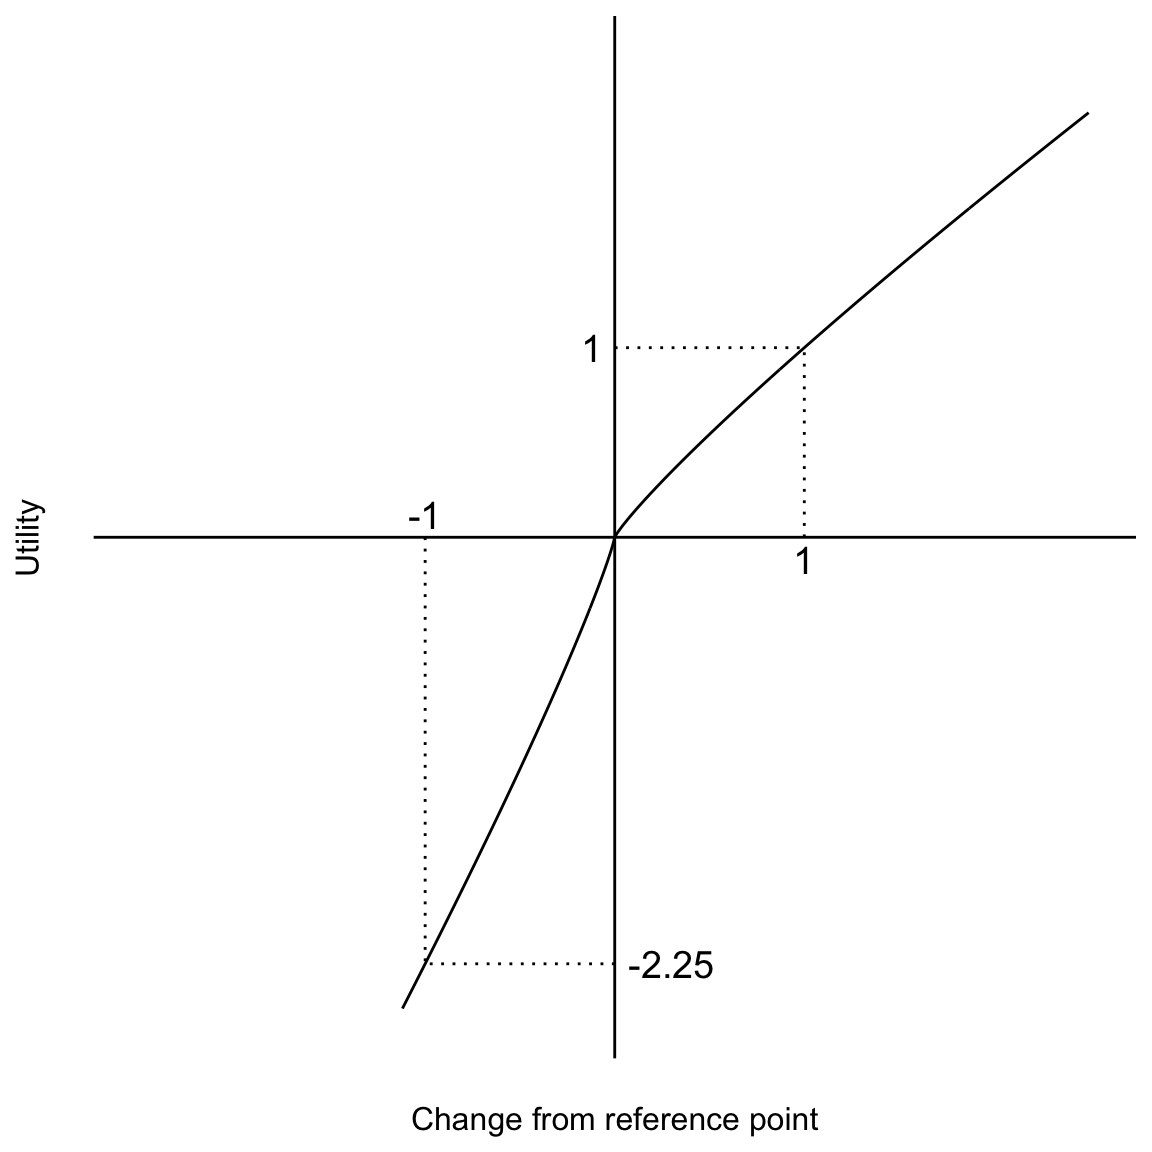
\includegraphics[width=1\linewidth]{thesis_files/figure-latex/prospect-theory-1} \caption{The value function in Prospect Theory \autocite[adapted from][]{kahneman1979}. The values for the exponent representing the extent diminishing returns (\(\alpha\)) and the loss aversion coefficient (\(\lambda\)) were 0.88 and 2.25, respectively. These were the median values calculated by \textcite{tversky1992} from experimental data.}\label{fig:prospect-theory}
\end{figure}

In plain language, loss aversion means that losses have more impact than
equivalent gains. In fact, the impact of loss aversion can be expressed even
more precisely, as a measurement of the ratio of the slopes of the curve for
gains and losses. This measure tells us the average amount that losses have more
impact than equivalent gains. In a sequel to the original prospect theory paper,
\textcite{tversky1992} measured a median coefficient of 2.25 of loss aversion. This means
that people respond to losses 2.25 times more than equivalent gains.
Figure~\ref{fig:prospect-theory} shows this disparity. Equivalent changes in
actual wealth from the references point (x-axis) have different impacts on the
changes' subjective value (y-axis). An increase in wealth (+x) brings about an
increase of value (+y). However, a decrease in the same amount of wealth (-x)
brings about a decrease in value 2.25 times the value of the equivalent gain
(-2.25y). The straight lines adjacent to the curves showcase that the function
is steeper in the loss domain than it is in the gain domain. This difference of
slope is another indicator of loss aversion.

This research is relevant to resource allocation because managers often need to
evaluate project proposals that involve an element of risk. Therefore, managers
are likely to be affected by similar effects on risk that have been shown in
laypeople. However, hierarchical organisations offer an even more complex
situation. \textcite{lovallo2020} found that the risk profiles of lower-level managers are
lower that those of the top managers. They suggest that this may be due to
lower-level managers' risk aversion to accepting projects that may jeopardise
their job. However, the top managers recognise that a loss in one or more
business units is likely to be offset by gains in other units. Such an
inconsistency in risk profiles across the levels of an hierarchical organisation
fails to take advantage of the benefits of risk aggregation, which has long been
understood in external markets \autocite{markowitz1952}. The psychological literature
shows that people's risk aggregation is facilitated through various choice
bracketing manipulations. However, there has been no work that investigated such
situations without providing participants with inter-trial feedback. The
experiments presented in Chapter~\ref{aggregation} investigate the effects of
choice bracketing on risk aggregation without feedback.

\hypertarget{project-similarity}{%
\subsection{Project similarity}\label{project-similarity}}

When evaluating project proposals, managers are likely to be influenced by the
relative similarity of the available options to each other. The extent to which
this may be true is important especially since the increase of diversified
firms. Organisations are not only varied by the number of divisions which they
possess, but also by the extent of diversification. This means that managers are
likely to find themselves comparing across dissimilar types of projects.

As mentioned above, there are likely many organisational and financial reasons
why the extent of diversification in an organisation would impact its
performance. However, the impact of psychological factors such as business
project similarity has not been investigated. This approach is important because
the relative similarity of projects has implications about how difficult the
evaluation process becomes and therefore what kind of financial metrics are
used. Having more similar projects to compare may mean more attributes on which
to evaluate, whereas a dissimilar comparison may lead to a situation in which a
manager has to rely on potentially unreliable metrics.

Structure-mapping theory \autocites[SMT;][]{gentner1997,gentner1983} provides a model of
comparison that psychologically distinguishes similar and dissimilar allocation
tasks. SMT models comparison as a process of bringing conceptual structures into
alignment, which when possible, puts shared component dimensions into
correspondence. Alignment both highlights when two conceptual structures share
dimensions, but also highlights how the two structures differ along those shared
dimensions, called \emph{alignable differences}. For example, when comparing two oil
discovery projects, all the relevant processes of planning an exploration and
measuring the amount of hydrocarbons in a prospect might be identical, but the
specific amount measured will be different. This is the alignable difference: a
difference between the two projects that is constrained within the same
conceptual structure. However, when comparing between an oil field and a
refinery, there will be significantly more \emph{non-alignable differences}, because
the two domains do not share component dimensions. That is, many of the
processes that exist in the exploration business unit have a significantly
different dimensional structure to those in the refinery business unit, such
that it will be difficult to find meaningful alignments. More non-alignable
differences mean that there are less opportunities to make meaningful
comparisons, and so would make predicting project success and ranking their
priority more difficult. In Chapter~\ref{alignment}, I experimentally examined
business project comparisons and how project alignment affects resource
allocation decisions.

When evaluating projects, managers make use of financial metrics, such as NPV.
However, such metrics are reliant on forecast estimates of, for instance, future
cash flows. Do managers take into account inherent such variance in their
decisions? This is especially important to investigate given the above
discussion. In cases of non-alignable comparison managers might be relying on a
potentially unreliable metric. On the other hand, in an alignable comparison,
managers might have the option to moderate their choice based on the relative
reliability of different metrics. It is important to remember that all such
decisions are often very consequential for the manager. That is, the project
could ultimately make the company money and lead to future opportunities for the
manager, or potentially cause financial harm to the company (and subsequently
lead to a job loss).

Psychological research shows that laypeople are in general quite poor at using
numerical variance information \autocite{galesic2010,konold1993,vivalt2018,batteux2020}. However, it is unclear to what extent managers would be sensitive
to variance information in the metrics associated with the projects that they
evaluate. On the one hand, perhaps managers' financial training will allow a
consideration of such variance estimates, but this might not manifest in a
situation in which managers have already been shown to be prone to biases. In
Chapter~\ref{alignment}, I investigate whether people are as sensitive to
verbally-instructed reliability information as they are to numerical reliability
information.

\hypertarget{reasoning-from-past-cases}{%
\subsection{Reasoning from past cases}\label{reasoning-from-past-cases}}

Managers often use past events to reason and make predictions about the future
\autocite{einhorn1987}. Such past events may be those that happened to the individual
manager, a case from the organisation's history, or from an external source.
This will especially be the case in a project evaluation scenario when a given
project is hard to compare with the other projects at hand. However, managers
evaluating project proposals may make inappropriate comparisons when considering
the target project to other cases. For instance, people tend to limit the sample
size of the set of comparison cases to a target problem to a small number. Often
only a handful of cases, or even one. Doing this might mean only considering
surface similarity to the current situation and not an alignment of the
underlying causal structure. Further, this might mean not considering other
similar projects.

\textcite{tversky1974} discussed a number of biases that may influence such processes. The
availability bias is seen when people mistake the ease of retrieval of
information for its frequency. Further, research on analogical retrieval showed
that people are more likely to retrieve surface similar cases than those with a
relational connection \autocite{gentner1993}. As such, managers are likely to recall
cases that may not be sufficiently relevant to their target situation and be
overly-confident about the frequency of such cases occurring. Such a focus on a
particular case might then also lead to an anchoring effect, wherein other
decisions might be disproportionately seen as relevant. \textcite{tversky1974} also found
that people are not sensitive to properties of sample size such as the greater
amount of non-representative outcomes in small samples. This means that managers
are even less likely to appreciate the importance of considering a large sample
of cases when drawing conclusions to a target problem. \textcite{tversky1974} also note an
insensitivity to predictability, in which people do not take into account the
reliability of the information that they have to make a prediction. This might
mean that managers may struggle to ideally weigh evidence of varying degrees of
reliability.

External sources that might be used to compare to a target situation include
business case studies. Considering such examples of prior business decisions or
events are the way that most MBAs learn about the business world. Publications
such as Forbes or Harvard Business Review publicise various businesses'
successes and failures and so may create an allure to use such case studies in
the decision-making process. On the other hand, managers may have access to more
aggregated data about their industry from, for instance, consultancy companies.
How do managers use these various types of evidence in their decision-making?

Research on this topic suggests that managers tend to prefer anecdotes over
statistics, unless aided \autocite{wainberg2018}. This is a concern because \textcite{gavetti2005}
suggests that managers often make use of case studies quite poorly. The analogy
literature draws a distinction between surface similarity, in which a mapping is
made between easily identifiable but potentially functionally irrelevant
attributes, and relational similarity, in which the underlying mechanism is
considered. Are managers sensitive to the deeper causal mechanisms that underlie
the anecdotes they judge? Or are they simply influenced by surface similarity?
In Chapter~\ref{anecdotes}, I investigate the extent to which people moderate
their reliance on anecdotes or aggregated data by the relevance of the anecdote
to the target project during resource allocation.

\hypertarget{chapter-overview}{%
\section{Chapter overview}\label{chapter-overview}}

In sum the potential consequences for a diversified hierarchical structure are
that projects will be consisdered one at a time, and if they are considered
togetherj, disparate project types will make comparisons hard. Considering
projects one by one might mean that risk is not aggregated across projects and
therefore value is lost. The difficultly to compare will lead to both
potentially relying on unreliable metrics, and relying on improper anecdotal
evidence. The thesis is that people often go half-way. They do not completely
disregard the normative strategy, but also struggle to moderate their decisions
when it comes to more subtle statistical principles such as aggregation,
variance, and sampling.

In the previous section I identified three resource allocation processes that
are currently under-studied and so are important to investigate further. First,
the evaluation of individual project proposals might lead to managers only
considering such projects one at a time, despite the opportunity of aggregating
a portfolio of such projects. The choice bracketing literature suggests that
there are ways of facilitating such aggregation, but does not investigate this
without providing participants inter-trial feedback. Second, in situations in
which managers compare multiple projects, the structural alignment literature
suggests that managers in diversified firms will struggle to allocate more than
those in more integrated firms. Further, these managers might not be sensitive
to the variance inherent in the financial metrics they rely on. Third, a
difficulty to compare across existing projects might instead mean a reliance on
prior case studies from personal or external experience. Research on anecdotal
bias suggests that managers might rely more on such case studies than on
aggregated data, but it is unclear whether they will use relevance to moderate
their decisions.

Therefore, I investigate the psychology of resource allocation decisions in
three chapters. In Chapter~\ref{aggregation} I investigate the effects of
choice bracketing on risk aggregation without feedback. In
Chapter~\ref{interstitial-1}, I discuss the difference between evaluating
project proposals with inherent budget estimates and the process of allocating
an existing budget top-down. In Chapter~\ref{alignment} I investigate the
effects of alignment and reliability type---verbal or numerical---on
allocations. In Chapter~\ref{interstitial-2}, I discuss the
trade-offs that people make when using information to evaluate options such as
project proposals. Finally, in Chapter~\ref{anecdotes} I investigate the effects
of anecdote similarity on the anecdotal bias.

\newpage

\printbibliography[segment=\therefsegment,heading=subbibintoc]



\begin{savequote}
Fortune sides with him who dares.
\qauthor{---Virgil}\end{savequote}

\hypertarget{aggregation}{%
\chapter{Effect of choice bracketing on risk aggregation in repeated-play gambles with no feedback}\label{aggregation}}

\chaptermark{Effect of choice bracketing on risk aggregation}

\minitoc

\hypertarget{introduction-1}{%
\section{Introduction}\label{introduction-1}}

Investors know not to put all their eggs in one basket. Ever since work on
modern portfolio theory \autocite{markowitz1952}, it has been clear that combining the
risk of a set of individual investments reduces the overall risk of the
portfolio of investments. But what about situations in which it is not clear
that a set of investments fit together as a portfolio? Personal decisions such
as buying a car or moving cities are typically evaluated independently, as are
business decisions such as a farm investing in new cropping technology or a
multi-business firm building a mine.

While these decisions are separated in time, they are often not so far apart
that it is easy to learn from past outcomes (and sometimes the outcomes
themselves are unclear). This is because the outcomes of large investments are
often delayed. As such, the decision-maker cannot always use the knowledge of
the returns of one investment when evaluating a subsequent investment. Any
results that a farmer may identify from using a new technology will only become
apparent after many seasons of use. Similarly, it will take many years for a
multi-business firm to begin to estimate whether the output of a mine resulted
in the expected return on investment. These are the decisions that I investigate
in this chapter: sequences of large risky choices without immediate outcomes.

Risk aggregation is the combination of probability and/or variance information
associated with certain outcomes for the purpose of understanding that
information more comprehensively \autocite{bjornsen2019}. However, the psychological
literature suggests that this process may be difficult for people. Work on
prospect theory \autocite{kahneman1979} suggests that people's evaluation of gambles
does not conform to expected utility theory and is prone to framing effects.
Specifically, people typically evaluate gambles one by one \autocite{rabin2009,tversky1981,kahneman1993}. As such, it is unlikely that people will be able
to aggregate risk when they do not perceive a series of investments as a
portfolio. So, what would encourage people to aggregate risk? The literature on
\emph{choice bracketing} \autocite{read1999} shows that grouping a set of individual gambles
together facilitates risk aggregation. As such, the current work provides two
primary contributions. First, I am the first to investigate the effect of choice
bracketing on risk aggregation in independent gambles evaluated without
immediate returns. Second, I introduce novel choice bracketing manipulations.

The earlier work on risk aggregation essentially did the aggregating work for
the participants. For example, experimenters provided participants with an
outcome probability distribution, and/or an explicit indication to group the
choices together, such as by asking for a single decision to be made on a set of
identical gambles. Other work addressed the more realistic situation of a set of
independent gambles. However, most of this work provided participants with the
outcomes of their choices before the subsequent choice. In these paradigms
participants experienced individual outcomes from the eventual outcome
distribution of the gambles, meaning that aggregation was confounded with
learning. As mentioned above, in real-life there is usually a significant delay
between the choice a person or firm makes and the outcome of that choice, and
there are likely to be several interim choices in the meantime. This is
especially true for business executives, who would typically have to wait months
or years before beginning to understand the consequences of their decision, and
even then the outcome may be unclear. However, previous work did not investigate
the effect of choice bracketing on risky choice without feedback. This is
surprising, since choice bracketing is exactly the kind of process that should
promote aggregation in these more realistic decisions. As such, I investigated
new ways of encouraging participants to bracket their risky choices, but with a
paradigm that involves a series of independent choices without feedback. In this
way, my paradigm is more isometric with real-life risky choice.

\hypertarget{multi-play-gambles}{%
\subsection{Multi-play gambles}\label{multi-play-gambles}}

Despite the difficulties of risk aggregation, people seem to aggregate ``naively''
when considering multiple gambles. \textcite{samuelson1963} told of a colleague who
rejected a gamble that involved a 50\% chance of gaining \$200 and a 50\% of losing
\$100, despite the gamble's positive Expected Value (EV). That is, \(200 \cdot 0.5 - 100 \cdot 0.5 = +50\). Rejection of a positive EV gamble out of fear of the
possible loss is classic loss aversion. However, the same colleague said he
would accept 100 plays of the same gamble. \textcite{samuelson1963} argued that this
choice is irrational, but other work suggests that it is consistent with
expected utility theory when certain assumptions are clarified \autocites[e.g.,][]{ross1999,aloysius2007}. However, a normative discussion is out of the scope of the
present work. Intuitively, it is clear that over the course of 100 gambles, the
positive EV wins out, and a net loss of money is extremely unlikely. Samuelson's
colleague was more risk averse when making a single decision about one gamble (a
\emph{single-play} gamble), than when making a single decision about multiple
identical gambles (a \emph{multi-play} gamble).\footnote{I use the terminology from \textcite{bristow2011} and \textcite{camilleri2013} for
  consistency.}

\textcite{wedell1994} replicated the \textcite{samuelson1963} anecdote experimentally with a gamble
involving a potential gain of \$100 and a potential loss of \$50. Participants
accepted the multi-play gamble of 100 plays more than the single-play gamble.
This effect has since been replicated with different outcomes and probabilities,
both with hypothetical and real money. Some participants often require fewer
than 10 plays of a previously rejected gamble in order to accept it \autocite{dekay2005,keren1991,montgomery1982,redelmeier1992}. Other similar studies found a
multi-play effect that was in the predicted direction but not significant
\autocite{barron2003,benartzi1999,klos2005,langer2001}. Further, the effect is not
seen when participants do not perceive gamble outcomes as fungible \autocite{dekay2006,dekay2005,dekay2011} or when choice is continuous rather than discrete
\autocite{bristow2011}.

However, multi-play effects are likely robust, since there is also evidence that
such gambles reduce a variety of cognitive biases, such as common-ratio effects
\autocite{keren1987,keren1991,dekay2006}, preference reversals \autocite{wedell1990},
ambiguity aversion \autocite{liu2009}, and the illusion of control \autocite{koehler1994}.
Participants are also more likely to use explicitly provided EVs in multi-play
gambles \autocite{li2003}, show eye movements more congruent with an EV model than
single-play gambles \autocite{su2013}, and judge multi-play gambles as riskier
\autocite{joag1990}.

Multi-play gambles that are displayed with an aggregated outcome distribution
(that presents the probabilities of all the different possible outcomes) of
those gambles are accepted more than multi-play gambles without these
distributions \autocite{benartzi1999,redelmeier1992,klos2013,webb2017,coombs1971,venkatraman2006,dekay2005,langer2001,keren1991} because they
very clearly show the rarity of a loss. Note that this does not seems to hold
when returns are calculated as percentages, rather than fixed dollar amounts
\autocite{stutzer2013}; and when participants do not perceive gamble outcomes as
fungible \autocite{dekay2005}. However, when this effect is demonstrated, the multi-play
gamble is usually set up such that its (binomial) outcome distribution shows a
relatively low chance of losing any money and a very low chance of losing a lot
of money. For instance, Figure~\ref{fig:samuelson-distribution-10} shows the
outcome distribution of the \textcite{samuelson1963} gamble played 10 times. These kinds
of outcome distributions do the aggregating work for the participants, making
the attractiveness of the multi-play gamble clearer. This work suggests that
participants can comprehend and respond to aggregated risk, but that they
struggle to compute the aggregation without external help.



\begin{figure}
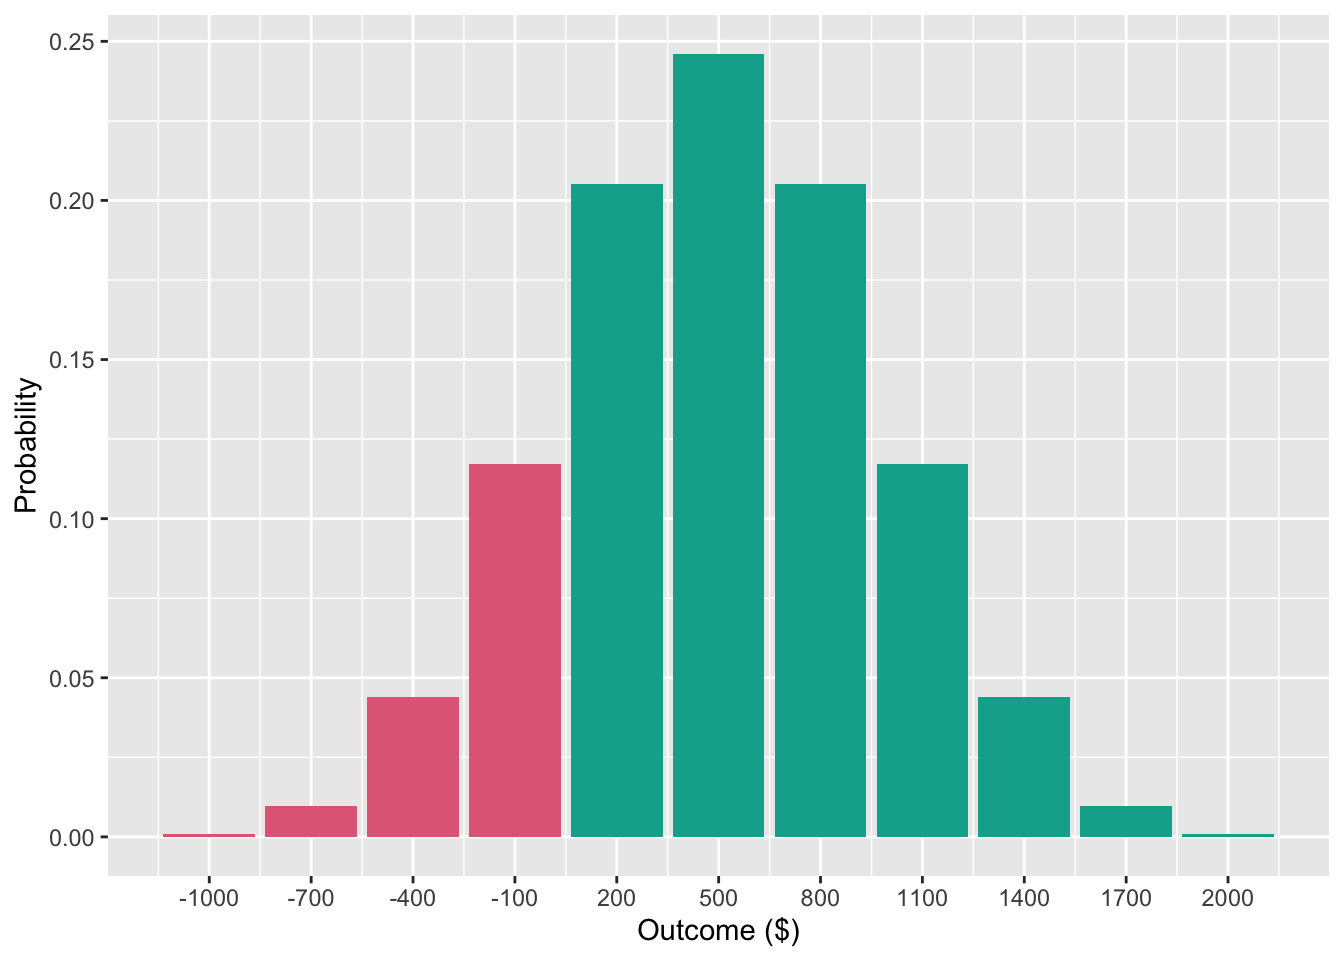
\includegraphics[width=1\linewidth]{thesis_files/figure-latex/samuelson-distribution-10-1} \caption{The outcome probability distribution of the \textcite{samuelson1963} gamble (0.5, 200; 0.5, -100) played 10 times.}\label{fig:samuelson-distribution-10}
\end{figure}

\hypertarget{repeated-play-gambles}{%
\subsection{Repeated-play gambles}\label{repeated-play-gambles}}

Decisions in real life are usually sequential, and rarely identical as in the
multi-play paradigm \autocite[cf.][]{barron2003}. That is, people tend to be confronted
with individual choices whose outcomes and outcome probabilities are different
from one choice to another, and these choices occur at different points in time.
In a business setting this can be seen in decisions about whether to invest in
new projects; proposals and opportunities differ widely and occur at different
times. Managers are not ever simply asked: ``Here are 10 identical investments to
consider; do you want all or none of them?''

In \emph{repeated-play} (rather than multi-play) gamble paradigms, participants make
decisions about a series of different gambles. Research using this paradigm
found that people are less risk averse when outcomes for a series of gambles are
evaluated and decisions are made less frequently \autocite{gneezy1997,thaler1997,bellemare2005,beshears2016}. People are also less risk averse (for positive
EV gambles) when they receive feedback or are able to sample from a distribution
before making a choice \autocite{camilleri2011,camilleri2013,barron2003,wulff2018,ludvig2011,hertwig2004,jessup2008}. Other work found that loss
aversion is mitigated when people are explicitly instructed to consider the
options as a part of a portfolio \autocite{sokolhessner2009,sokolhessner2012}.

These studies are closer to real-life decisions than the multi-play gamble
paradigm, because they involve a set of separate gamble decisions, rather than a
single decision about a set of gambles. However, for the most part, the
experiments used in the repeated-play gamble literature use various forms of
feedback throughout the course of the experiment. That is, participants are
shown the outcomes of their gambles before they make more decisions. This
paradigm is known as \emph{experience-based choice}. In \emph{description-based choice},
on the other hand, the gamble is simply presented to the participant without any
feedback, as in the multi-play gambles above. In real life, people rarely see
the immediate outcomes of their risky choices, and even less so in business
settings, where any return on investment often takes years to manifest.

Only a limited number of studies have used a repeated-play paradigm without
feedback. For instance, \textcite{jessup2008} and \textcite{hertwig2004} investigated the effects of
feedback in repeated-play gambles on the weighting of small probabilities, so
therefore had a no-feedback control condition. Other work similarly used
individual description-based gambles presented sequentially \autocites[e.g.,][]{ert2013,joag1990}. However, these studies did not attempt to facilitate participants'
risk aggregation. \textcite{haisley2008} provided limited evidence for facilitating risk
aggregation. They gave participants the opportunity to buy five (negative EV)
lottery tickets, and either presented them one at a time, or together.
Participants bought fewer tickets, thereby maximising EV, when they considered
them jointly. However, the experimenters did not specify the outcomes and
probabilities of each gamble, meaning that it is unclear if participants
understood the independent lotteries as identical or non-identical. This reduces
the external validity of the study, as most independent risky choice involves
non-identical outcomes and probabilities. In sum, these studies were not
designed to research how to facilitate risk aggregation and reduce loss
aversion.

\hypertarget{choice-bracketing}{%
\subsection{Choice bracketing}\label{choice-bracketing}}

Research in psychology and economics has identified ways of facilitating risk
aggregation by encouraging people to group their choices. Specifically, people
aggregate more when they consider the consequences of their choices together
(broad bracketing) than when they consider them individually \autocite[narrow bracketing;][]{read1999}. In multi-play gambles (especially when displayed with an outcome
distribution), choices are inherently bracketed broadly because a single choice
is made about multiple gambles. Similarly, studies that used repeated-play
gambles facilitated risk-tolerance essentially through broad bracketing. For
instance, when \textcite{thaler1997} presented gamble outcomes less frequently, they
allowed participants to consider longer time increments with a single
evaluation.

The goal of this chapter is to facilitate risk aggregation without the
experimental artefact of immediate feedback. Previous research suggests some
ways of doing this. \textcite{sokolhessner2009} and \textcite{sokolhessner2012} found that lengthy
instructions with an elaborate explanation to ``think like a trader'' -- and to
consider all the repeated-play gambles as a portfolio, as opposed to considering
them individually -- reduced risk aversion. Further, even the original
\textcite{samuelson1963} anecdote (and its subsequent replications) show that people do
have an intuition for aggregation even without the risk being calculated exactly
for them. I am interested in testing whether that same intuition can be elicited
and applied across sets of unique bets. What are the minimal conditions required
to encourage aggregation? Both this explicit instruction effect and the
multi-play gamble work suggest that participants can engage in a more intuitive
form of aggregation when provided with the right contextual cues. It might be
the case that people possess such an intuitive understanding, and that simply
being encouraged to consider a set of choices together in more subtle ways than
explicit instruction will also facilitate aggregation. This could involve simply
making participants aware that they are going to be making a series of choices.
This kind of contextual cue may be sufficient to encourage risk aggregation.
Investigating the effects of more subtle cues will help shed light on the
cognitive processes underlying choice bracketing. Of course, the effects of more
subtle cues would not eliminate the utility of explicit financial education, but
they will help the design of decision-making contexts to best align with such
instruction.

In addition to simply informing participants that they will make a series of
choices, making the choices more readily comparable may facilitate broad
bracketing, and thus risk aggregation. Consider the inverse situation wherein a
lack of comparability between choices may prevent broad bracketing, such as when
an executive for a multi-business firm makes decisions across multiple distinct
industries. Of course, the similarity of decision contexts does not change the
maths of risk aggregation, and but may well affect whether people do aggregate
risk across decisions. \textcite{dekay2005} found that multi-play effects are not seen
when choices are not considered fungible. For instance, participants aggregated
across dollar amounts, but not across patients in a medical decision. As such,
people may behave similarly when considering a set of dissimilar choices,
insofar as they consider them not fungible.

There is further suggestive evidence that the similarity of a set of choices to
one another will affect choice bracketing. Choices whose differences are easy to
compare (alignable differences) are weighted heavier than those that are
difficult to compare \autocite{markman1995,markman2010}. Increased similarity across a
set of choices may both highlight the ability for those choices to be bracketed,
and further facilitate risk aggregation through the comparable attributes.
However, it is possible that increased similarity will facilitate risk
aggregation even without a tangible benefit to the underlying calculations. That
is, it is possible that simply manipulating the similarity of
financially-irrelevant semantics of a choice set that people will become less
risk averse. If so, then this will be by virtue of an implicit risk aggregation
in which the mere awareness of the possibility of a grouping of choices reduces
risk aversion. It is important to investigate the effect of similarity
especially because in managerial settings, executives in multi-business firms
will often have to make comparisons across industries that are hard to compare.
For instance, General Electric currently develops both analytic software
products and jet engines for the military. They had been even more diversified
previously, at one stage simultaneously developing home appliances and owning
the NBC television network.

In addition to the similarity between choices, how choices are presented may
affect how easily they are compared, and thus whether or not the multiple
subsequent effects listed above would come to fruition. As mentioned above,
\textcite{haisley2008} found a higher degree of EV maximisation when gambles were
presented jointly, rather than separately. Similarly, \textcite{hsee1999} found that
people's choices were affected by whether they viewed the attributes of the
choices separately or jointly. Their \emph{evaluability hypothesis} suggests that
attributes that are difficult to evaluate will have a greater impact on joint
presentation than separate presentation. Joint presentation is a form of broad
bracketing because it forces a participant to view of all the components of a
decision together. Participants may therefore be more likely to consider
aggregating the risk involved in a set of choices when all those choices are in
view. Joint presentation potentially reduces the working memory load otherwise
needed to maintain those set of choices. As such, it is quite possible that a
combination of highly similar choices, presented jointly will lead to the
highest likelihood of broad bracketing, and thus risk aggregation.

\textcite{moher2010} replicated \textcite{gneezy1997}, but separately manipulated the number of
gambles seen per trial and feedback frequency. They found that participants were
less risk averse when viewing a set of three gambles per trial, than when
viewing only one. However, they only found this effect with a set of identical
outcomes. When outcomes were non-identical, there was no effect of presentation.
However, participants were always presented with gamble outcomes for each trial,
so it is unclear to what extent this influenced participants' ability to bracket
broadly. In fact, when seeing gambles separately, participants were less risk
averse when receiving feedback for each trial, compared to every three trials.
Testing a presentation manipulation without the confound of feedback will help
to clarify this effect.

\hypertarget{internal-market-capital-investment-context}{%
\subsection{Internal market capital investment context}\label{internal-market-capital-investment-context}}

Executives of large, successful firms are often viewed as fearless risk-takers
who take on risky projects to generate innovation and growth. However, the
available evidence suggests that executives do not view themselves that way
\autocite{swalm1966,march1987}. Executives typically evaluate multiple investments
over time. Risk aggregation is sensible when investments are only partially
correlated (i.e., the success of one does not influence the success of another).
It is sensible to take on a set of risky investments with positive EV, where
each investment has some chance of loss, because those that succeed will make up
for those that failed. These benefits are well-known in stock market investment
settings, thanks to Nobel laureate Harry Markowitz's work on modern portfolio
theory \autocite*{markowitz1952}.

However, it is unclear whether the general public and even business managers use
this principle, due to the extent of risk aversion in both those populations
\autocites[e.g.,][]{tversky1992,march1987}. In fact, executives treat risk like the rest
of us; they view investments one at a time, are risk averse for gains and risk
seeking in the domain of losses \autocite{maccrimmon1986,swalm1966,lovallo2020}.
However, it is understandable why risk aggregation is foreign to most people;
outside of an investment portfolio selection situation, it is unlikely for
people to group a selection of individual risky choices. Usually in life, people
encounter risky choices sequentially, and so the risk of each individual choice
is more salient than the aggregated risk of an arbitrary combination of choices.

\textcite{lovallo2020} show that executives treat investments within their own company in
isolation. In multi-business firms, the managers of each business unit often
make the investment decisions about individual projects. As such, they often do
not consider the scope of their decisions in the context of the entire company.
For instance, Nobel laureate Richard Thaler offered 25 division managers working
for the same firm a hypothetical investment that involves a 50\% chance of
gaining \$2 million for the company and a 50\% chance of losing \$1 million. Only
three managers said they would accept the investment \autocite{thaler1999}. However, the
CEO indicated that he would have clearly preferred managers to accept all the
investments. To each middle-manager, the choice represents a risk of loss for
their division and potentially their job, whereas for the CEO the entire
portfolio of choices represents a worthwhile risk.

In this chapter I investigate risky choice in the context of business project
investment internal to a company because this is a real-world context where
choice bracketing is important and currently under-utilised \autocite{lovallo2020}. The
participants in my studies were taken from a general population that does not
have extensive managerial experience. However, in the general population a lack
of risk aggregation is most likely more common, and the variables I am
researching here are readily applicable to the financial decisions that lay
people make. For instance, one of the real-world applications of the choice
bracketing literature has been to use outcome distributions and increased time
horizons to encourage investment in high risk, but high EV, retirement funds
\autocite[e.g.,][]{benartzi1999}. Otherwise, people typically prefer low risk, low EV,
funds. Further, because my task concerns managerial decision-making, I can
investigate contextual cues to choice bracketing, while eliminating potential
differences between participants in their prior experience with the specific
decision-context. Future research will focus on managers with
context-specific experience to investigate the effects of that experience.

\hypertarget{experiment-1}{%
\section{Experiment 1}\label{experiment-1}}

In Experiment 1, I investigated the effect of three choice bracketing
manipulations on risky choice in hypothetical resource allocation scenarios.
Previous research had low ecological validity because of the use of multi-play
paradigms or feedback. In this experiment, the risky choice task was a
description-based repeated-play paradigm, meaning that participants had to make
a choice about whether to accept a number of different hypothetical investments,
but were not provided with feedback about their choices. I manipulated the
similarity of the choices, whether they were presented together or separately,
and whether participants were aware of the number of choices that they would be
making.

The values and probabilities of the gambles were set up such that each
individual gamble, as well as the aggregation of all the gambles, would be
attractive to a rational agent interested in maximising EV. As such, the key
dependent measure was the proportion of risky choices participants accept.

Previous research suggests that people will exhibit more risky choice when
explicitly told to bracket their choices \autocite{sokolhessner2009,sokolhessner2012},
when choices are presented jointly \autocites[e.g.,][]{moher2010,hsee1999}, and when
choices are similar \autocites[e.g.,][]{dekay2005,markman1995}. Therefore, I tested the
following hypotheses:

\begin{hypothesis}
\protect\hypertarget{hyp:awareness-aggregation-1}{}{\label{hyp:awareness-aggregation-1} }Participants that know how many projects to expect will make more risky choices
than participants that are unaware.
\end{hypothesis}

\begin{hypothesis}
\protect\hypertarget{hyp:presentation-aggregation-1}{}{\label{hyp:presentation-aggregation-1} }Participants will make more risky choices when seeing projects jointly than when
seeing them separately.
\end{hypothesis}

\begin{hypothesis}
\protect\hypertarget{hyp:similarity-aggregation-1}{}{\label{hyp:similarity-aggregation-1} }Participants that see projects from the same industry will make more risky
choices than participants that see projects from different industries.
\end{hypothesis}

\hypertarget{method}{%
\subsection{Method}\label{method}}

\hypertarget{participants}{%
\subsubsection{Participants}\label{participants}}

One hundred and ninety-eight (82 female) people were recruited from the online recruitment platform Prolific. Participants were compensated at a rate of £5 an hour. The average age was 32.52 (\emph{SD} = 11.42, \emph{min} = 18, \emph{max} = 69). Participants reported an average of 7.01 (\emph{SD} = 9.1, \emph{min} = 0, \emph{max} = 42) years of work in a business setting, and an average of 1.7 (\emph{SD} = 2.85, \emph{min} = 0, \emph{max} = 20) years of business education. The mean completion time was 12.04 (\emph{SD} = 11.29, \emph{min} = 3.1, \emph{max} = 112.4) minutes.~Table~\ref{tab:condition-allocation-aggregation-1}
shows the between-subjects condition allocation.

\begin{table}[tbp]

\begin{center}
\begin{threeparttable}

\caption{\label{tab:condition-allocation-aggregation-1}Experiment 1 group allocation.}

\begin{tabular}{lll}
\toprule
Similarity & \multicolumn{1}{c}{Awareness} & \multicolumn{1}{c}{N}\\
\midrule
High & Aware & 53\\
High & Naive & 53\\
Low & Aware & 47\\
Low & Naive & 45\\
Total & - & 198\\
\bottomrule
\end{tabular}

\end{threeparttable}
\end{center}

\end{table}

\hypertarget{materials}{%
\subsubsection{Materials}\label{materials}}

\hypertarget{instructions-materials-aggregation-1}{%
\paragraph{Instructions}\label{instructions-materials-aggregation-1}}

Participants were told to imagine that they are executives in a large company
and that they will need to decide about investing in a number of hypothetical
business projects. Appendix~\ref{instructions-materials-aggregation-1-appendix}
shows a screenshot of these instructions.

\hypertarget{task-aggregation-1}{%
\paragraph{Risky investment task}\label{task-aggregation-1}}

In the risky investment task, participants saw 10 short descriptions of business
projects, and were asked whether they would invest in that project or not. Each
description included the name of the hypothetical business, the amount they
forecast the project to cost, the amount they forecast the project to make, and
probabilities for these forecasts. I constructed these projects to appear
attractive when aggregated, and unattractive when segregated \autocite[see][]{langer2001}.
Project values were different for each project, but followed a set of
constraints for each project's EV and the probability of any loss given the
outcome distribution of all 10 projects (\(P(loss)\)). Further, there was a
constraint on the gambles' loss aversion coefficient (\(\lambda\)), which is the
ratio of potential gains over the potential losses. The constraints were:

\begin{enumerate}
\def\labelenumi{\arabic{enumi}.}
\item
  \(\text{EV} > 0\);
\item
  \(\lambda < 2.25\); and
\item
  \(P(loss) < 0.1\).
\end{enumerate}

As such, each project cannot be considered to be a loss under expected value
theory, but also would not be an easy choice for investment, because of the low
\(\lambda\) \autocite[made to be lower than the median loss aversion coefficient calculated
in][]{tversky1992}. Further, since people are especially sensitive to loss
probabilities \autocite{zeisberger2020,kahneman1979}, an arbitrarily low \(P(loss)\) was
chosen to make investment in the complete set of projects seem attractive. The
actual probability of a loss given the outcome distribution I used was
0.09. This was calculated by summing all
probabilities in the Poisson binomial distribution whose outcomes were less than
zero. For comparison, \(P(loss)\) =
0.17 for 10 plays of the \textcite{samuelson1963}
gamble. Figure~\ref{fig:project-choice-aggregation-1} shows an example of a
description of a project in this task.



\begin{figure}
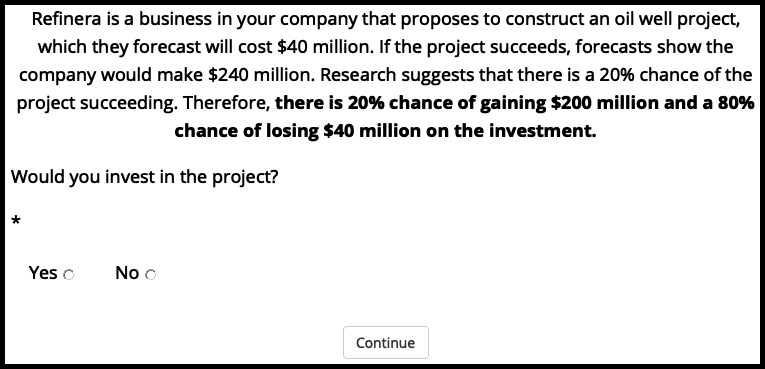
\includegraphics[width=1\linewidth]{thesis_files/figure-latex/project-choice-aggregation-1-1} \caption{Example of a project choice display in Experiment 1. Border added for clarity.}\label{fig:project-choice-aggregation-1}
\end{figure}

In the high similarity condition, these project descriptions were all about one
type of project (in this case an oil well project) and were all from the same
business. In the low similarity condition, each project was from a different
industry. In the joint presentation condition, the 10 projects were all
displayed on the one webpage, whereas in the separate presentation condition
each was displayed on a different webpage. Participants in the aware condition
saw the display shown in Figure~\ref{fig:awareness-aware-aggregation-1} before
their separate presentation display. Those in the naive condition simply
proceeded without this message. Note, the financial and probability values were
identical regardless of condition, and the order of each set of 10 projects was
randomised.



\begin{figure}

\includegraphics[width=1\linewidth]{thesis_files/figure-latex/awareness-aware-aggregation-1-1} \caption{The display seen by those in the aware condition of Experiment 1. Border added for clarity.}\label{fig:awareness-aware-aggregation-1}
\end{figure}

Although the project descriptions are succinct, and the decisions in the task
are made quickly, they reflect real decisions in businesses in critical ways.
Companies that consider their forecast estimates probabilistically (i.e., do not
simply use the most likely estimate as the only estimate) do in fact frame their
options as likelihoods of certain monetary outcomes.

\hypertarget{outcome-distribution-materials-aggregation-1}{%
\paragraph{Outcome distribution decision}\label{outcome-distribution-materials-aggregation-1}}

Participants were asked if they would invest in the last 10 projects they saw
and were provided with a graph of the outcome probability distribution of the 10
projects. Appendix~\ref{outcome-distribution-materials-aggregation-1-appendix}
shows this graph. After collecting data I discovered that there was a coding
error in the generation of gambles, which meant that I could not make use of the
outcome distribution decision data. Therefore, the effect of outcome
distribution will not be discussed until \protect\hyperlink{aggregation-2}{Experiment 2}, in
which I fixed this issue. Appendix~\ref{outcome-distribution-aggregation-1}
presents an analysis of this data, and describes the coding error and its
implications.

\hypertarget{follow-up-gambles}{%
\paragraph{Follow-up gambles}\label{follow-up-gambles}}

Participants were shown four further sets of gambles (11 total) that functioned
to check participant attention and replicate the gambles from \textcite{samuelson1963} and
\textcite{redelmeier1992}. See Appendix~\ref{follow-up-materials-aggregation-1-appendix}
for details.

\hypertarget{procedure}{%
\subsubsection{Procedure}\label{procedure}}

Participants read the instructions and completed the risky investment task,
first in the separate presentation condition, and then in the joint condition.
Participants then made the outcome distribution decision, responded to the 11
follow-up gambles.

\hypertarget{results-aggregation-1}{%
\subsection{Results}\label{results-aggregation-1}}

\hypertarget{project-choice}{%
\subsubsection{Project choice}\label{project-choice}}

I conducted a three-way ANOVA to investigate the effects of similarity,
awareness, and presentation on the proportion of participants' decision to
invest in the 10 projects. As seen in
Figure~\ref{fig:plot-aggregation-1-awareness}, participants invested more when
they were told that there will be 10 projects, compared to when they were not
told this, \(F(1, 194) = 9.52\), \(p = .002\), \(\hat{\eta}^2_p = .047\). As seen in
Figure~\ref{fig:plot-aggregation-1-presentation}, participants invested more
when viewing the projects jointly, compared to when they viewed them separately,
\(F(1, 194) = 28.14\), \(p < .001\), \(\hat{\eta}^2_p = .127\). Although there was no main effect of
similarity, \(F(1, 194) = 1.63\), \(p = .204\), \(\hat{\eta}^2_p = .008\), the interaction between
similarity and presentation was significant,
\(F(1, 194) = 4.31\), \(p = .039\), \(\hat{\eta}^2_p = .022\) (see
Figure~\ref{fig:plot-aggregation-1-similarity-presentation}). Specifically, the
presentation effect seems stronger in the high similarity condition,
\(\Delta M = 0.07\), 95\% CI \([0.04,~0.09]\), \(t(194) = 5.29\), \(p < .001\), than in the low similarity
condition, \(\Delta M = 0.03\), 95\% CI \([0.00,~0.05]\), \(t(194) = 2.06\), \(p = .041\).



\begin{figure}
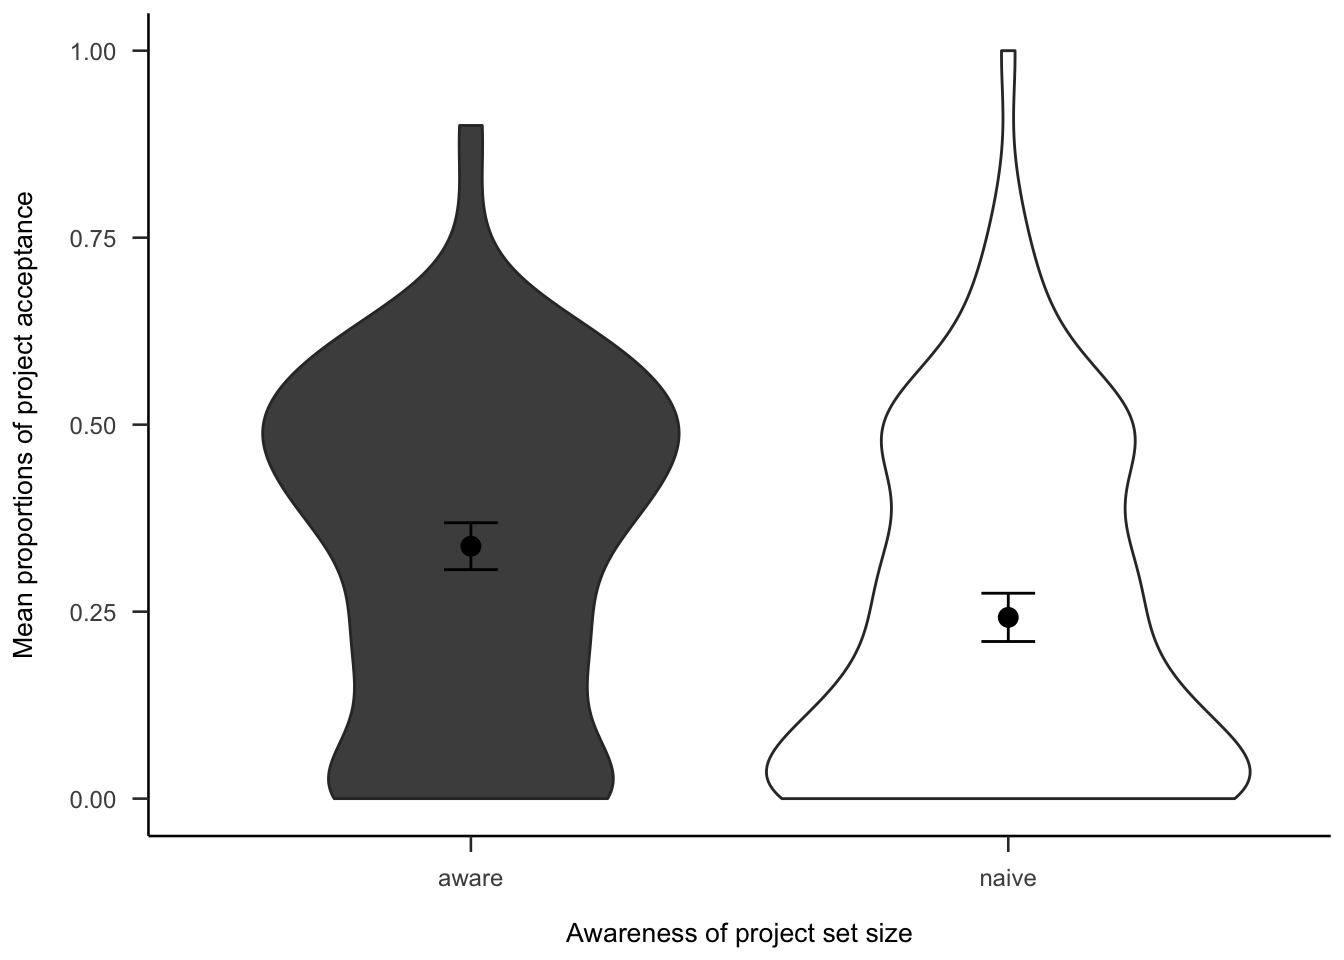
\includegraphics[width=1\linewidth]{thesis_files/figure-latex/plot-aggregation-1-awareness-1} \caption{Mean proportions of decisions to invest in each set of 10 projects, by awareness conditions. Error bars represent 95\% confidence intervals.}\label{fig:plot-aggregation-1-awareness}
\end{figure}



\begin{figure}
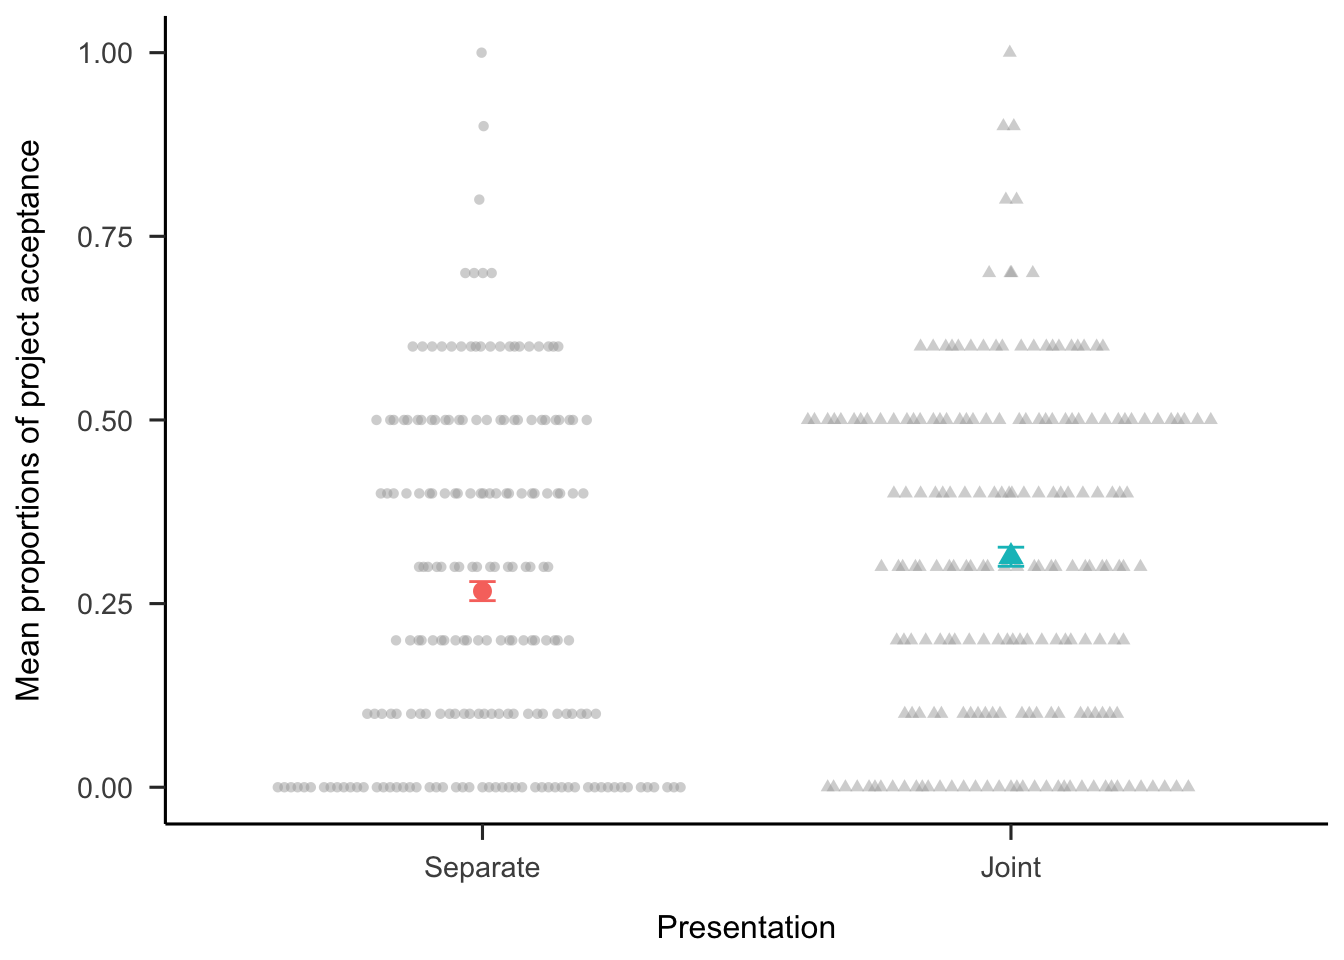
\includegraphics[width=1\linewidth]{thesis_files/figure-latex/plot-aggregation-1-presentation-1} \caption{Mean proportions of decisions to invest in each set of 10 projects, by presentation conditions. Error bars represent 95\% confidence intervals.}\label{fig:plot-aggregation-1-presentation}
\end{figure}



\begin{figure}
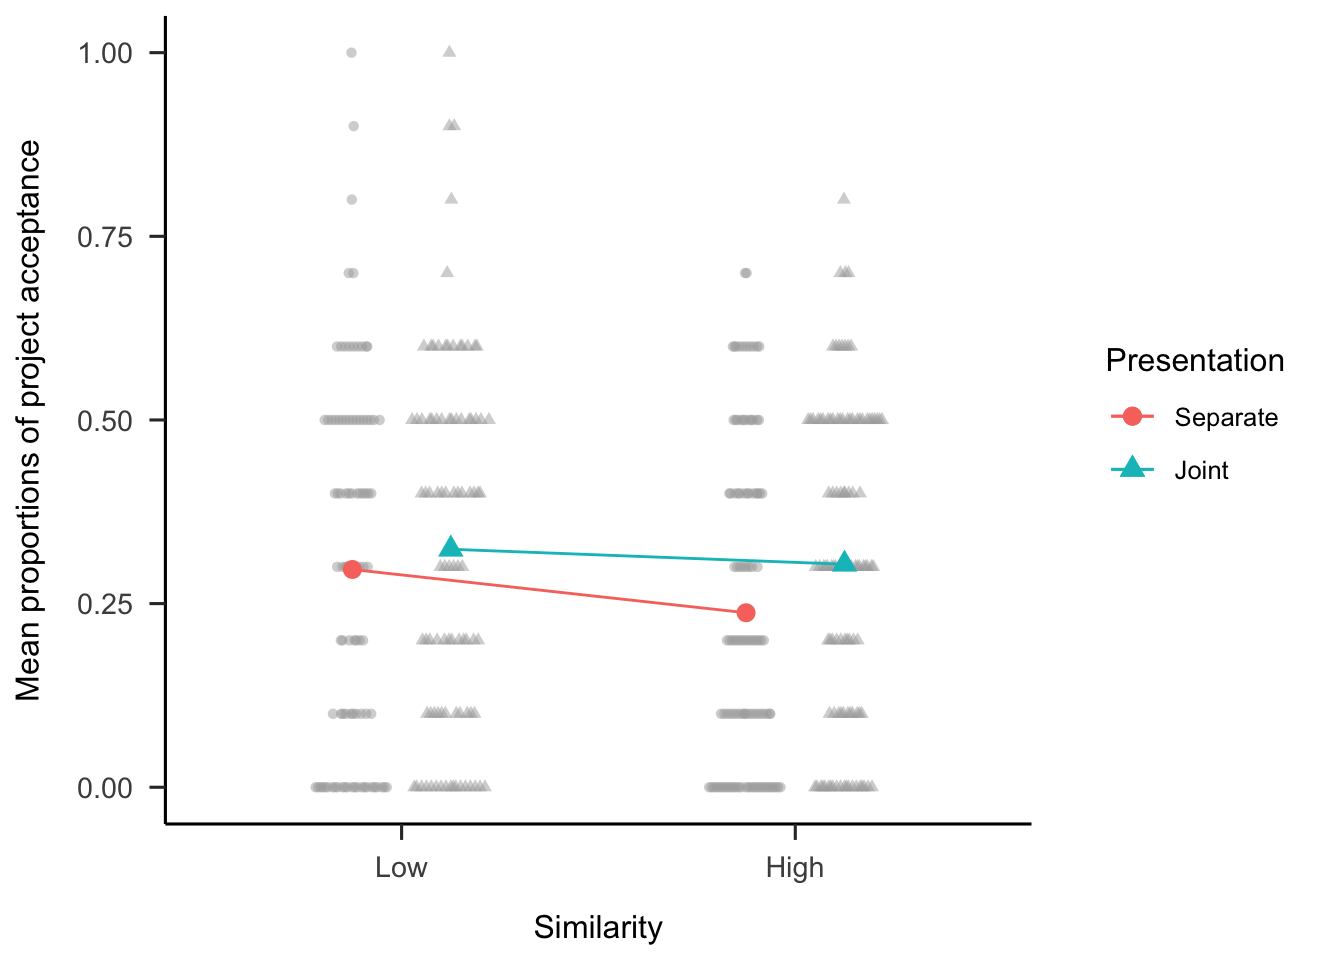
\includegraphics[width=1\linewidth]{thesis_files/figure-latex/plot-aggregation-1-similarity-presentation-1} \caption{Mean proportions of decisions to invest in each set of 10 projects, by similarity and presentation conditions. Error bars represent 95\% confidence intervals.}\label{fig:plot-aggregation-1-similarity-presentation}
\end{figure}

\hypertarget{trial-by-trial-analysis}{%
\subsubsection{Trial-by-trial analysis}\label{trial-by-trial-analysis}}

I conducted exploratory analyses into the possible effects of the manipulations
on a trial-by trial basis. Appendix~\ref{trial-by-trial-aggregation-1} shows
the data for all conditions. The key findings is in the separate presentation.
As Figure~\ref{fig:plot-aggregation-1-trials-separate-awareness} shows, in the
separate condition people are more likely to accept projects over the 10 trials,
but this interacts with awareness,
\(b = 0.04\), 95\% CI \([0.01, 0.08]\), \(z = 2.32\), \(p = .021\).
Specifically, the relationship between choice and trial is significant in the
aware condition,
\(b = 0.11\), 95\% CI \([0.06, 0.16]\), \(z = 4.54\), \(p < .001\); but not in the
naive condition,
\(b = 0.03\), 95\% CI \([-0.03, 0.08]\), \(z = 1.01\), \(p = .311\).



\begin{figure}
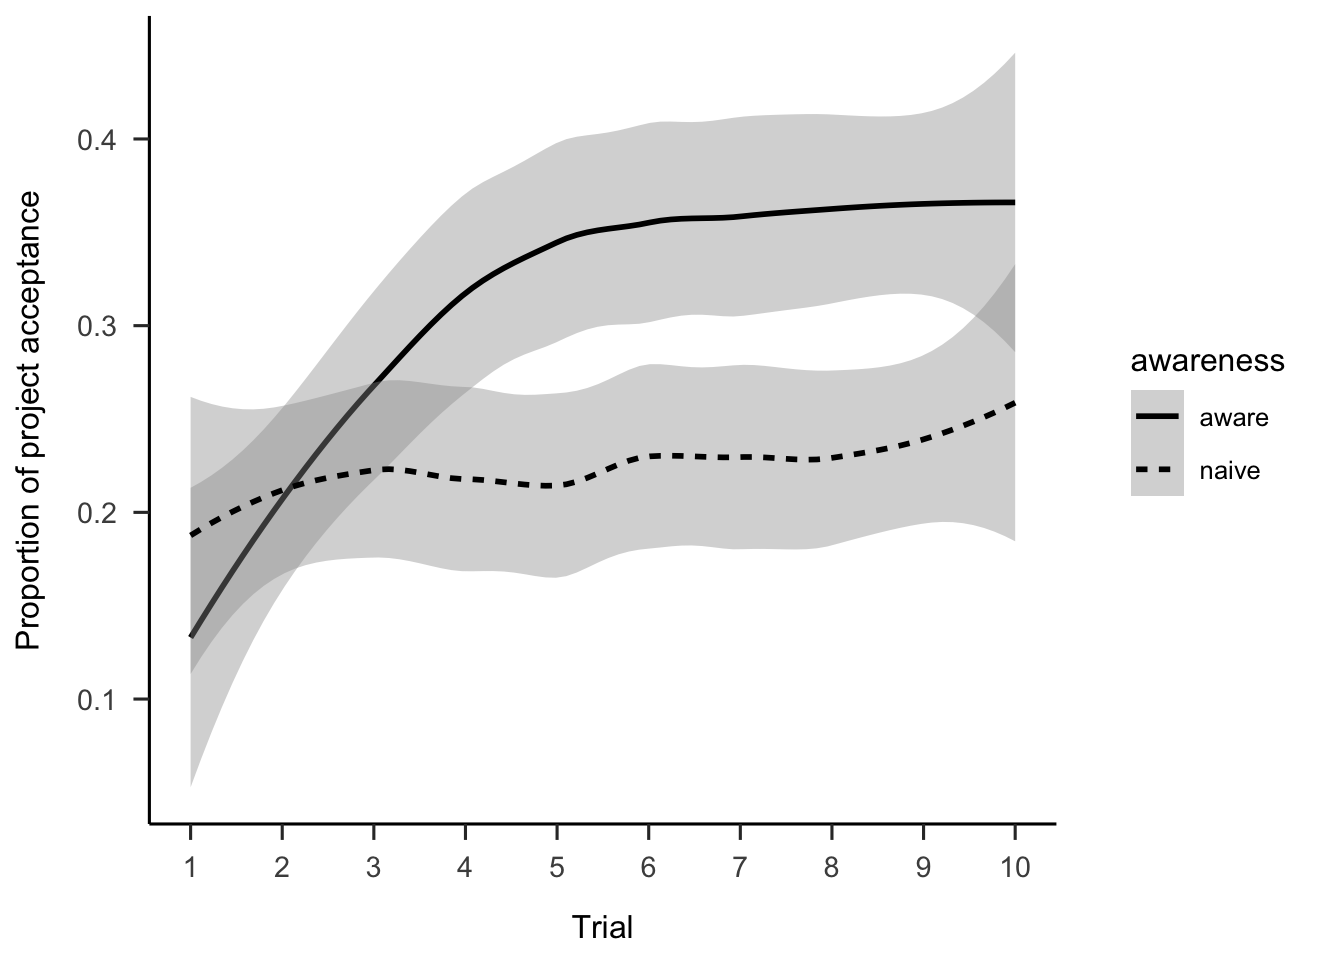
\includegraphics[width=1\linewidth]{thesis_files/figure-latex/plot-aggregation-1-trials-separate-awareness-1} \caption{Proportion of project acceptance in the separate presentation condition, by trial, and awareness conditions. LOESS is used for smoothing over trials, and the shading represents 95\% confidence intervals.}\label{fig:plot-aggregation-1-trials-separate-awareness}
\end{figure}

\hypertarget{discussion-aggregation-1}{%
\subsection{Discussion}\label{discussion-aggregation-1}}

I found evidence for most of the Experiment 1 hypotheses. Specifically, I found
that people make more risky choices when considering those choices jointly on
the same page, compared to on separate pages; and when they know how many
choices were in the set. Further, I found an interaction between project
similarity and presentation, and found tentative evidence that people are less
risk averse when risky choices are aggregated for them. Exploratory analyses
showed that participants' risk aversion seemed to decrease as they proceeded
through the trials, but only when participants were aware of the number of
projects.

\hypertarget{presentation-effect}{%
\subsubsection{Presentation effect}\label{presentation-effect}}

The presentation effect may be a result of one of two mechanisms. A mathematical
aggregation explanation would mean that participants are combining the gambles
into a mental representation of the probability distribution and then deciding
based on the attractiveness of that distribution. A joint presentation of
choices would facilitate this combination. On the other hand, people may also be
using a sort of ``naive'' aggregation process when they are encouraged to group
their choices together. A naive aggregation explanation would suggest that
participants in the joint condition are simply more likely to realise that a few
big wins could offset a few losses. It may be the case that participants were
encouraged by the joint display to consider the set of projects together, and
perhaps conclude that ultimately investing in a higher number of gambles is
potentially valuable due to the possibility that one project might pay off the
projects that showed losses.

\hypertarget{awareness-effect}{%
\subsubsection{Awareness effect}\label{awareness-effect}}

I found an awareness effect such that participants that viewed the projects
separately, were more likely to invest in the projects as the trials went on,
regardless of the actual gambles. It might be the case that having an awareness
of the total number of projects in the set would increase the likelihood that
participants would naively aggregate. Specifically, knowing the number of total
projects might make the idea that the gains of some projects will offset the
losses of others will be more salient, because it reinforces a focus on the
entire set.

Otherwise, this result may also be due to the Gambler's fallacy/law of small
numbers. This effect is characterised by people's expectation of a pattern to
follow the underlying distribution of the function that generates each
component. For instance, someone observing the results of a coin flip that look
like HTTHTTTT might anticipate that the likelihood of ``heads'' is higher than
that of a ``tails,'' despite the actual likelihood being 50\% for either. This
effect occurs in sequential decision-making, so may be relevant for the
repeated-play decisions in Experiment 1. \textcite{barron2010} found that the gambler's
fallacy (in a roulette prediction task) emerges when information about past
outcomes was displayed sequentially, but not when it is displayed all at once.
\textcite{haisley2008} found evidence for the gambler's fallacy with a repeated-play
gamble paradigm. As such, it is possible that a Gambler's fallacy-type effect
can explain the effect of the awareness manipulation. That is, participants may
have thought that after a few gambles that they considered risky, the last ones
were more likely to materialise. Further, this would be more likely to occur for
those that knew the total number of projects, because they knew when the
sequence was approaching its end.

\hypertarget{similarity-discussion-aggregation-1}{%
\subsubsection{Similarity effect}\label{similarity-discussion-aggregation-1}}

I did not find a main effect of similarity in the individual choice data as
predicted in Hypothesis~\ref{hyp:similarity-aggregation-1}. I found that
choice similarity interacted with the presentation condition. This interaction
is harder to explain since I did not originally hypothesise it. In fact, the
results seem to suggest the opposite to what was originally expected. Initially,
I predicted that people would be less risk averse in the high similarity
condition, due to the better ability to consider the isolated projects as a set.
I thought that more similarity would act as a broad bracket, and therefore
increase aggregation. That is, I would have expected that seeing a set of
similar projects would help participants aggregate risk when seeing them
separately, more than when projects are dissimilar. Instead, project acceptance
was actually numerically (but not statistically) higher in the low than in the
high similarity condition when projects were presented separately, averaging
over awareness conditions.

There was no significant difference between similarity conditions regardless of
presentation condition. However, joint presentation condition allocated
significantly more than those in the separate condition for both high and low
similarity. The interaction seems to have been found due to this difference
being larger in the high similarity condition. As such, the presentation effect
can be interpreted as having benefited from a joint presentation more when
projects were all from the same industry than when they were from different
industries. Perhaps the ability to aggregate risk when projects are presented
together is more made more salient when projects are similar.

Specifically, the interaction seems to be driven by the separate high similarity
condition being lower, rather than by the joint high similarity being higher, as
would have been expected. As such, it may be the case that participants were
engaging in a naive \emph{diversification}, rather than a naive aggregation. In
``true'' diversification, people would choose a set of projects that are partially
(and ideally negatively) correlated, as per \textcite{markowitz1952}. However, in reality
to the extent that people diversify, they seem to only diversify naively,
meaning that they neglect co-variation when diversifying \autocite[e.g.,][]{hedesstrom2006}. That is, they could be said to be looking for variety, rather
than diversification in the strict sense. This ``diversification bias'' is also
seen in product choices \autocite{read1995}.

In Experiment 1, participants may have considered the high similarity condition
a sign that the set of projects may not be sufficiently ``diversified.'' However,
this explanation would also predict the joint presentation condition to be lower
in the high similarity condition. So, it might be the case that those in the
separate condition were constantly thinking that they might be getting a
different project in the next display, so rejected more projects because of the
lack of diversification, but not realising that they would not be getting any
other type of project. Those in the joint presentation, on the other hand, were
able to see all ten projects, so would already known that there were no other
projects in the set, and so were less likely to reject projects on the basis of
the hope for different projects in the future.

\hypertarget{limitations}{%
\subsubsection{Limitations}\label{limitations}}

This experiment had two major limitations. First, proper counterbalancing was
not used in project domains, nor in the order of the within-subjects
manipulation of presentation. As such, it is unclear what role these elements
played in the results, especially in the presentation condition, in which
participants always saw the separate condition first. Second, as mentioned
\protect\hyperlink{outcome-distribution-materials-aggregation-1}{above}, there was a mistake in the
generation of the gamble values that meant that the individual gambles did not
correspond with the distribution that participants saw. Experiment 2 replicated
the effects from this experiment in the high similarity condition, so addressed
the second issue. Experiment 2 addressed the counterbalancing issue by adding
more project domains.

\hypertarget{experiment-2}{%
\section{Experiment 2}\label{experiment-2}}

Experiment 2 investigated the effect of presentation, awareness, and
distribution on project choice. For the distribution manipulation, I presented
half of the sample an outcome probability distribution as in the previous
literature \autocites[e.g.,][]{redelmeier1992,webb2017} to determine their risk aversion
when the gambles are explicitly aggregated. In contrast to repeated-play choice
literature, each choice was presented without feedback. Further, in contrast to
Experiment 1, I displayed this distribution alongside each gamble, as opposed to
only at the very end. This is an important manipulation because finding out
whether it is effective will 1. add to the understanding of the conditions
necessary for mathematical aggregation (beyond a mere intuitive sense of
aggregation), and 2. suggest new ways to encourage aggregation in real-world
applications.

In past work, participants were shown ordinary binomial distributions, since
multi-play gambles are identical. To my knowledge, there has not been an
investigation of \emph{non-identical} gamble distributions in this context. Doing
this requires using a \emph{Poisson} binomial distribution, which allows for multiple
trials with different probabilities.

Further, I addressed one of the limitations of Experiment 1 detailed
\protect\hyperlink{discussion-aggregation-1}{above} by manipulating all the main variables
between-subjects. By manipulating presentation between-subjects, I take out the
potentially confounding factor of reduced risk aversion over time.

I tested Hypotheses~\ref{hyp:awareness-aggregation-1},
and~\ref{hyp:presentation-aggregation-1}, from Experiment 1. Following the
finding in Experiment 1 that participants in the aware condition seemed to
become more risk-taking as the experiment progressed, I tested the following
hypothesis:

\begin{hypothesis}
\protect\hypertarget{hyp:awareness-trials-aggregation-2}{}{\label{hyp:awareness-trials-aggregation-2} }Participants will make more risky choices as the trials progress, but only when
they are aware of the total number of projects in the set.
\end{hypothesis}

Further, multi-play gambles with outcome distributions have been shown to reduce
risk aversion compared to multi-play gambles without distributions \autocites[e.g.,][]{redelmeier1992,webb2017}. Therefore, I tested the following hypothesis:

\begin{hypothesis}
\protect\hypertarget{hyp:distribution-aggregation-2}{}{\label{hyp:distribution-aggregation-2} }Participants will make more risky choices when presented with an aggregated
outcome distribution than when making the same decisions individually.
\end{hypothesis}

\hypertarget{method-1}{%
\subsection{Method}\label{method-1}}

\hypertarget{participants-1}{%
\subsubsection{Participants}\label{participants-1}}

One hundred and sixty-five (52 female) people were recruited from the online recruitment platform Prolific. Participants were compensated at a rate of £5 an hour. The average age was 26.33 (\emph{SD} = 8.64, \emph{min} = 16, \emph{max} = 72). Participants reported an average of 2.54 (\emph{SD} = 5.33, \emph{min} = 0, \emph{max} = 43) years of work in a business setting, and an average of 1.67 (\emph{SD} = 2.93, \emph{min} = 0, \emph{max} = 20) years of business education. The mean completion time was 6.51 (\emph{SD} = 5.13, \emph{min} = 1.18, \emph{max} = 39.93) minutes.~Table~\ref{tab:condition-allocation-aggregation-2}
shows the between-subjects condition allocation.

\begin{table}[tbp]

\begin{center}
\begin{threeparttable}

\caption{\label{tab:condition-allocation-aggregation-2}Experiment 2 group allocation.}

\begin{tabular}{llll}
\toprule
Awareness & \multicolumn{1}{c}{Distribution} & \multicolumn{1}{c}{Presentation} & \multicolumn{1}{c}{N}\\
\midrule
Aware & Absent & Separate & 41\\
Naive & Absent & Joint & 41\\
Naive & Absent & Separate & 41\\
Naive & Present & Separate & 42\\
Total & - & - & 165\\
\bottomrule
\end{tabular}

\end{threeparttable}
\end{center}

\end{table}

\hypertarget{materials-1}{%
\subsubsection{Materials}\label{materials-1}}

\hypertarget{instructions}{%
\paragraph{Instructions}\label{instructions}}

Participants were shown the same instructions as in
\protect\hyperlink{instructions-materials-aggregation-1}{Experiment 1}.

\hypertarget{task-aggregation-2}{%
\paragraph{Risky investment task}\label{task-aggregation-2}}

Participants saw a similar display to the one in
\protect\hyperlink{task-aggregation-1}{Experiment 1}, but with new gamble values, in order to fix
the mistake in the Experiment 1 gamble value calculation (detailed
\protect\hyperlink{outcome-distribution-aggregation-1}{above}).

The presentation and awareness manipulations were as in Experiment 1. However,
for the distribution variable, participants either saw the project descriptions
as is, or saw an outcome probability distribution of all the projects alongside
the description (see
Figure~\ref{fig:separate-distribution-present-aggregation-2}).



\begin{figure}
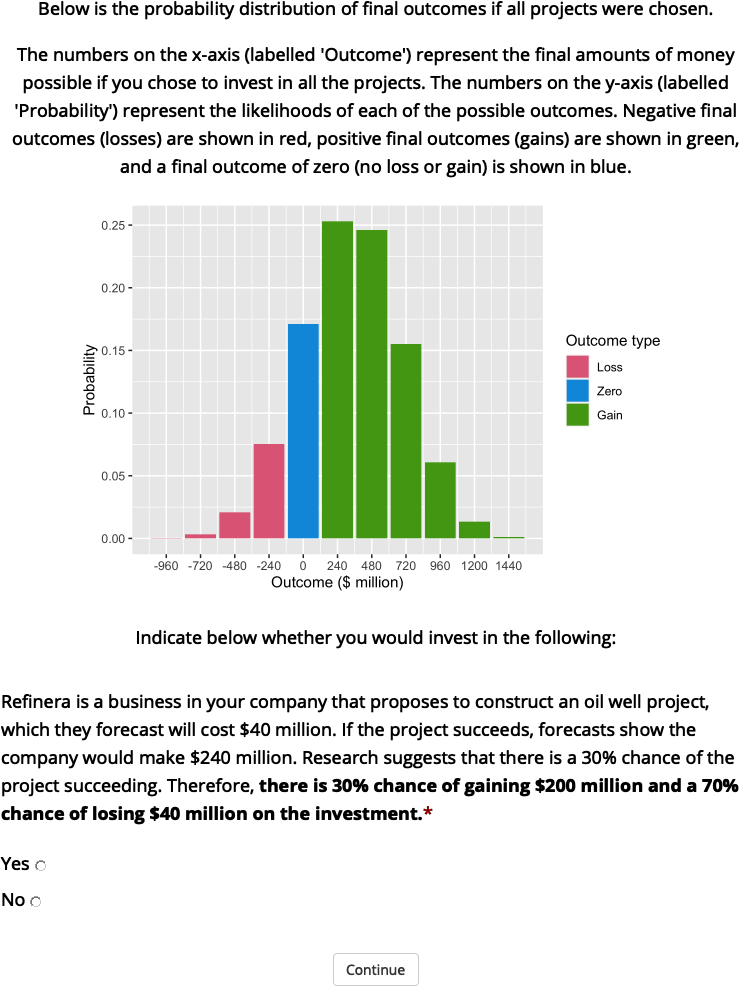
\includegraphics[width=1\linewidth]{thesis_files/figure-latex/separate-distribution-present-aggregation-2-1} \caption{An example of a display seen by those in the separate distribution-present condition of Experiment 2.}\label{fig:separate-distribution-present-aggregation-2}
\end{figure}

\hypertarget{follow-up-aggregation-2}{%
\paragraph{Follow-up}\label{follow-up-aggregation-2}}

I asked participants how many projects they think they saw, whether they were
willing to accept all or none of the projects, and how many they would
be willing to accept if they had to choose a number. See
Appendix~\ref{follow-up-materials-aggregation-2-appendix} for screenshots.

\hypertarget{procedure-1}{%
\subsubsection{Procedure}\label{procedure-1}}

Participants responded to demographic questions, read the instructions, and
completed the risky investment task in their respective conditions. After seeing
the individual projects, participants were then asked the three follow-up
questions.

\hypertarget{results-aggregation-2}{%
\subsection{Results}\label{results-aggregation-2}}

\hypertarget{project-investment}{%
\subsubsection{Project investment}\label{project-investment}}

The project investment data was analysed in two ways: as binary choice per trial
(using logistic regression), and as proportions of choice per participant (using
t-test). In each case I compared the relevant comparison condition to the same
control condition (separate naive distribution absent).
Figures~\ref{fig:plot-aggregation-2-choice}
and~\ref{fig:plot-aggregation-2-proportion} show the choice and proportion
data, respectively. The difference between presentation conditions was not
significant, both in the logistic regression
\(\hat{\beta} = -0.02\), 95\% CI \([-0.57, 0.53]\), \(z = -0.08\), \(p = .937\), and in the
t-test, \(d_s\) = 0.00, 95\% CI {[}-0.43, 0.43{]}, \(t\)(80) = 0.00, \(p\) = 1.000. Similarly, the
difference between awareness conditions was not significant, both in the
logistic regression \(\hat{\beta} = -0.25\), 95\% CI \([-0.86, 0.36]\), \(z = -0.79\), \(p = .428\),
and in the t-test, \(d_s\) = 0.17, 95\% CI {[}-0.26, 0.61{]}, \(t\)(80) = 0.78, \(p\) = .438. However,
those that that saw a distribution tended to choose to invest significantly more
(51.19\%) than those that did
not see a distribution
(39.02\%), seen both in the
logistic regression, \(OR = 1.88\), 95\% CI \([1.06, 3.35]\), \(z = 2.15\), \(p = .032\), and the
t-test \(d_s\) = 0.47, 95\% CI {[}0.03, 0.90{]}, \(t\)(81) = 2.11, \(p\) = .038.



\begin{figure}
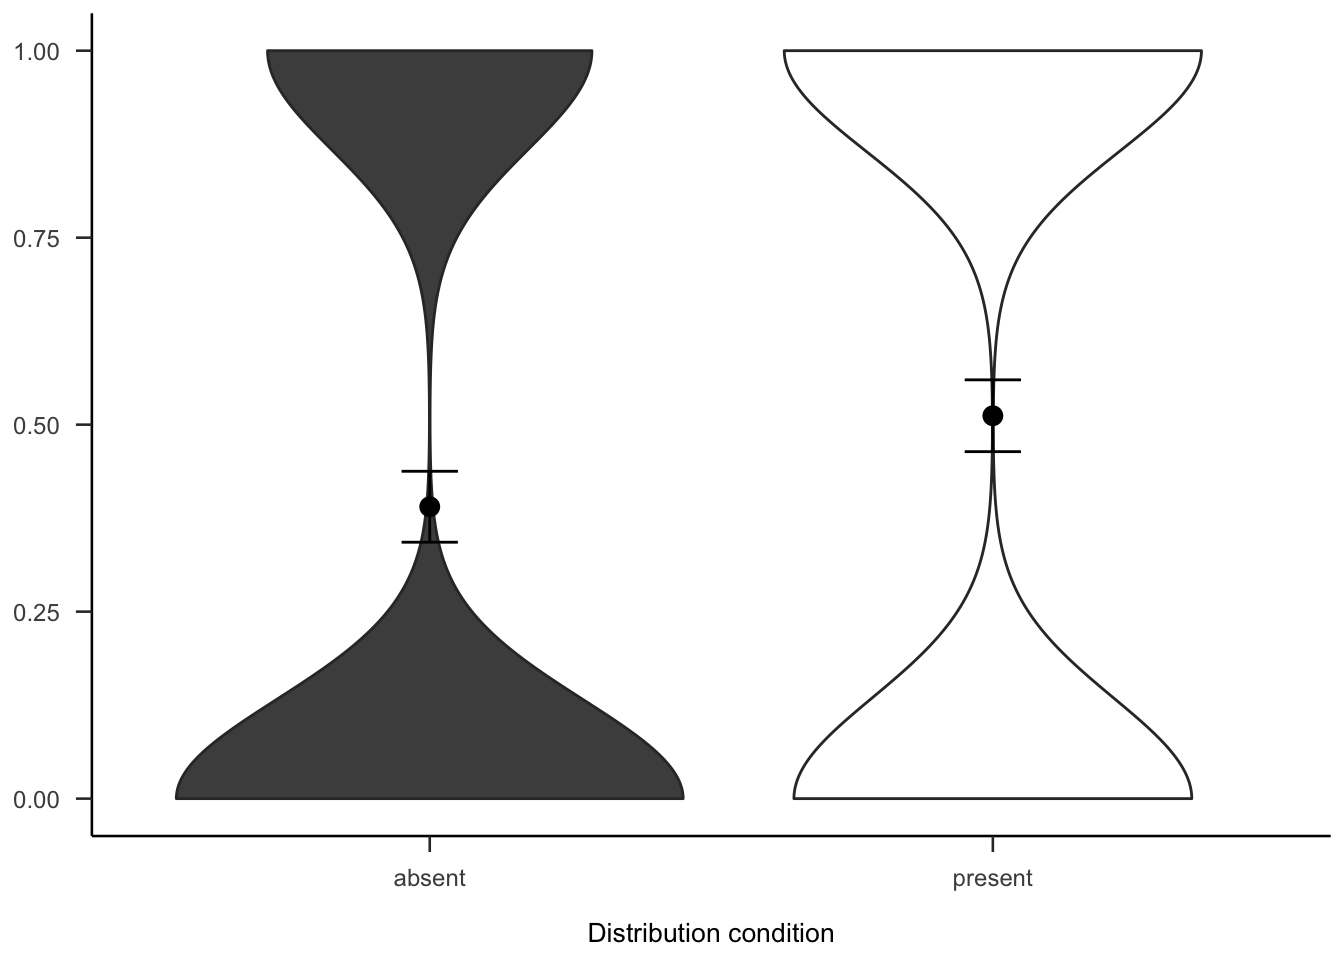
\includegraphics[width=1\linewidth]{thesis_files/figure-latex/plot-aggregation-2-choice-1} \caption{Mean project acceptance for the presentation, awareness, and distribution effects. Note, the condition on the left of each effect is the reference condition (separate presentation, naive awareness, distribution absent). As such, it is identical for the three effects.}\label{fig:plot-aggregation-2-choice}
\end{figure}



\begin{figure}
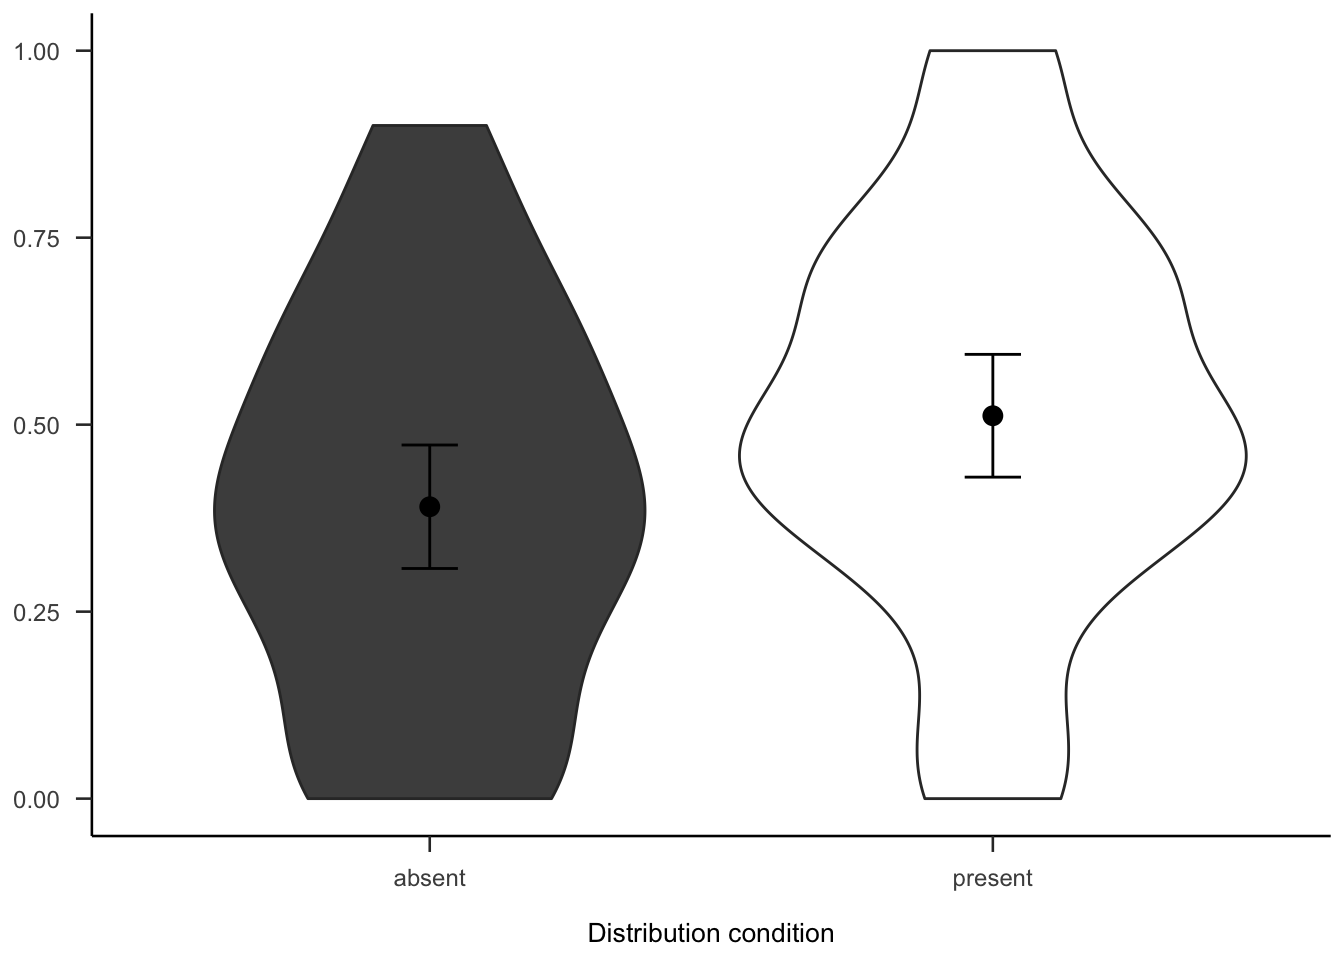
\includegraphics[width=1\linewidth]{thesis_files/figure-latex/plot-aggregation-2-proportion-1} \caption{Mean proportion of project acceptance for the presentation, awareness, and distribution effects. Note, the condition on the left of each effect is the reference condition (separate presentation, naive awareness, distribution absent). As such, it is identical for the three effects.}\label{fig:plot-aggregation-2-proportion}
\end{figure}

Further, as Figure~\ref{fig:plot-aggregation-2-choice-trials} shows, it
doesn't seem as if the previous awareness by trial effect was replicated.



\begin{figure}
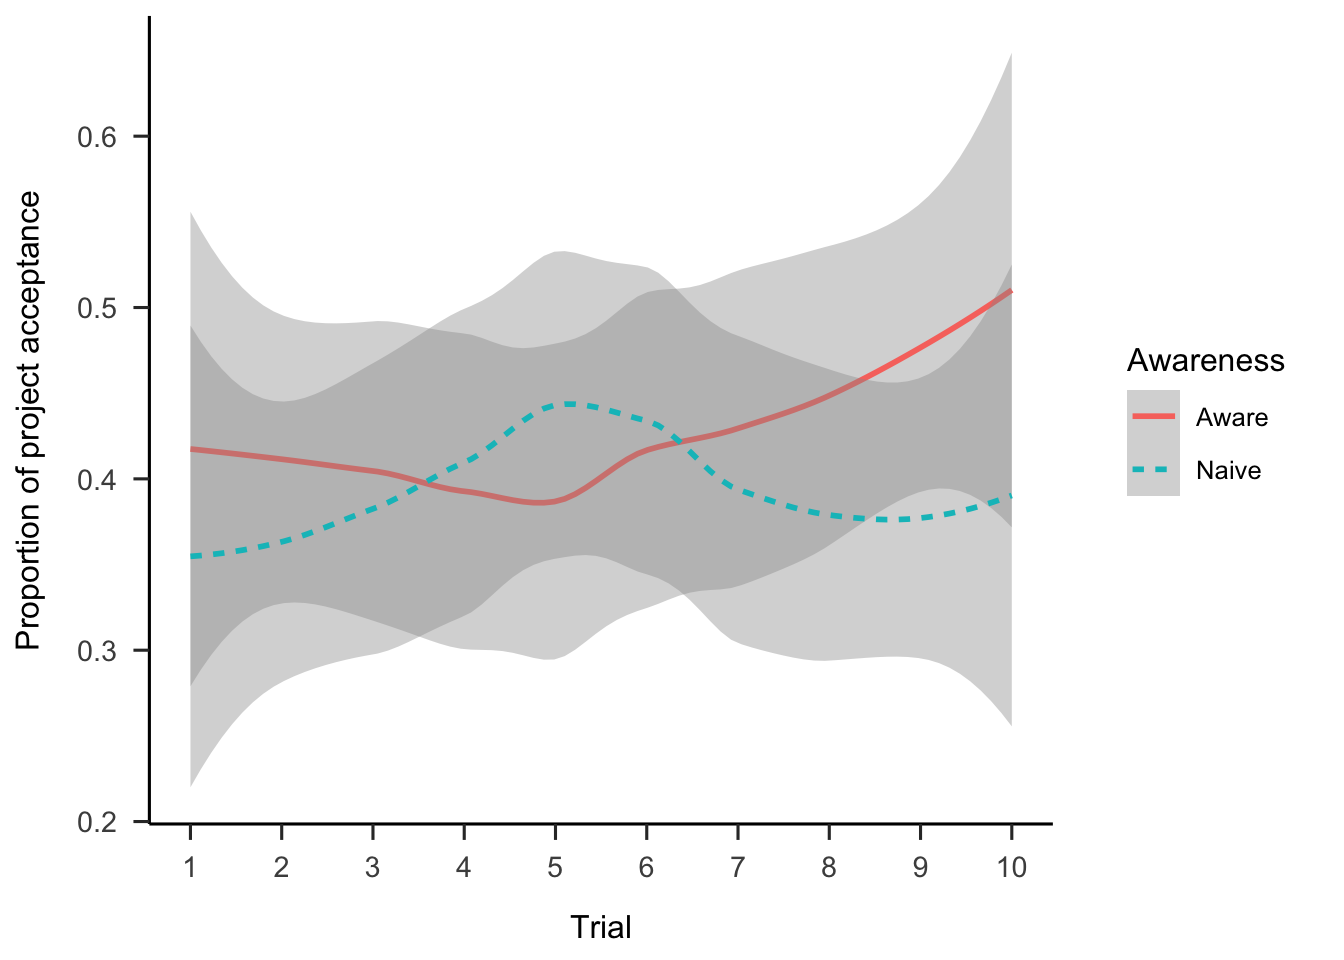
\includegraphics[width=1\linewidth]{thesis_files/figure-latex/plot-aggregation-2-choice-trials-1} \caption{Mean project acceptance for separate presentation, distribution absent condition, by awareness and trial.}\label{fig:plot-aggregation-2-choice-trials}
\end{figure}

\hypertarget{follow-up}{%
\subsubsection{Follow-up}\label{follow-up}}

The portfolio choice data from both the number and binary questions were
congruent with the above, finding that those in the distribution condition were
more likely to invest (see Appendix~\ref{results-aggregation-2-appendix}).

\hypertarget{discussion}{%
\subsection{Discussion}\label{discussion}}

I found support for one of the Experiment 2 hypotheses. Seeing an outcome
distribution of the projects had a strong effect on participants'
decision-making. Participants indicated that they would invest in more projects,
and were more likely to indicate that they would invest in the entire
``portfolio.'' However, the awareness and presentation effects I found in
\protect\hyperlink{results-aggregation-1}{Experiment 1} did not replicate.

The finding that seeing an outcome distribution of a set of gambles reduces risk
aversion for that set of gambles provides evidence for choice bracketing. That
is, people do seem to be primarily considering gambles one at a time.
Specifically in this case, this finding suggests that that the main bottleneck
for appropriately aggregating a set of gambles is a mathematical/computational
one. That is, people simply cannot mentally combine the outcomes and
probabilities in a way that sufficiently approximates the outcome distribution
display.

The lack of replication of the awareness and presentation effects provides
evidence against a naive aggregation account of the distribution effect.
Specifically this suggests that the distribution effect is a result of a lack of
ability to mathematically combine risk, rather than naive aggregation. If some
of the bottleneck was attributable to a lack of realisation that the individual
gambles could be grouped/bracketed together, then the effects from Experiment 1
should have replicated. However, instead it seems that even when people have an
opportunity to consider an entire set of risky choices together (and consider
that the gains may outweigh the losses), they do not do this.

In Experiment 2, all the gambles came from the same domain. I did this in order
to attempt to replicate the relevant effects from Experiment 1. However, it may
be the case that there was something about that particular domain that led to
the lack of replication. A follow-up experiment addressed this issue by
presenting participants with 20 gambles from 10 different industries and still
did not replicate the awareness effect (see Appendix~\ref{aggregation-4}).

\hypertarget{general-discussion}{%
\section{General discussion}\label{general-discussion}}

I found that choice bracketing facilitated risk aggregation in description-based
repeated-play gambles. This paradigm has never been a target of research. Early
work on risk aggregation involved multi-play gambles, which treated gambles as
simultaneous and identical. However, most risky choice outside the lab involves
considering multiple choices independently, as in repeated-play paradigms. Most
repeated-play paradigms have involved providing participants with feedback, or
allowing them to sample from outcome distributions. Large real-life investments
are different, as their outcomes are not eventuated immediately (and do not
allow for distribution sampling). The limited prior work using description-based
repeated-play gambles did not consider the effect of choice bracketing on risk
aggregation. As such, my paradigm allowed for the investigation of choice
bracketing in a way that is isomorphic with real-life prescriptions.

\protect\hyperlink{aggregation-1}{Experiment 1} found evidence for the effects of similarity,
presentation, and awareness of the number of projects. \protect\hyperlink{aggregation-2}{Experiment
2} found evidence for the effect of an outcome distribution but
did not replicate the presentation and awareness effects. Subsequent follow up
experiments (presented in Appendices~\ref{aggregation-3}
and~\ref{aggregation-4}) again tested the similarity and awareness effects. I
found evidence for naive diversification (an advantage for low similarity) when
considering them all projects once, and did not replicate the trial-by-trial
interaction from Experiment 1.

Therefore, in addition to the novelty of the paradigm itself, I found that
choice bracketing facilitates risk aggregation. As per
Hypothesis~\ref{hyp:distribution-aggregation-2}, I found that showing a
distribution of outcome probabilities without inter-trial feedback reduced risk
aversion. Further, I found mixed evidence for
Hypothesis~\ref{hyp:similarity-aggregation-1}, such that people were less risk
averse when the set of projects they saw were dissimilar, but only when offered
them as a portfolio. I found only minimal evidence for
Hypotheses~\ref{hyp:awareness-aggregation-1}
and~\ref{hyp:presentation-aggregation-1}, suggesting that viewing projects
together and awareness of the number of projects are not sufficient to encourage
aggregation. Altogether, it seems that subtle contextual cues are often not
sufficient to encourage risk aggregation, and that people need risk to be is
aggregated for them in order to understand the benefits of aggregation.

\hypertarget{theoretical-implications}{%
\subsection{Theoretical implications}\label{theoretical-implications}}

The finding that participants are less risk averse when provided with an
aggregated outcome distribution is congruent with previous work \autocite[e.g.,][]{redelmeier1992}. However, when distributions have been previously used,
gambles were identical in multi-play paradigms and used immediate feedback for
repeated-play paradigms \autocite[e.g.,][]{benartzi1999}. As I mentioned previously, both
these paradigms have limited ecological validity because usually people are
faced with non-identical sequential choices and do not receive immediate
feedback. I am the first to provide evidence for this aggregation effect with
non-identical gambles without feedback.

My other choice bracketing findings are less congruent with previous research.
\textcite{sokolhessner2009} and \textcite{sokolhessner2012} found that encouraging participants to
make decisions akin to a professional investor increased the amount of risky
choices they made. I found that subtler manipulation - whether or not
participants were aware of the number of choices to be made - is not sufficient
to encourage aggregation. \textcite{hsee1999} found that useful, but hard-to-interpret,
attributes were used more when the options were presented jointly, rather than
separately. In the case of these experiments, the ``hard to interpret'' element of
the decision set was the risk of the projects. Contrary to \textcite{hsee1999}, it seemed
that risk was not always accounted for more when projects were presented
jointly, rather than separately. More study is needed to understand whether the
effects that were seen in \protect\hyperlink{results-aggregation-1}{Experiment 1} but not
replicated in the subsequent experiments are due to statistical chance or
specific elements of the experiment.

Research on the effect of option similarity on choice \autocite[e.g.,][]{markman1995}
suggests that alignable differences are more important than non-alignable
differences. Further, the effects of multi-play gambles and outcome
distributions on risk aggregation are only seen when participants perceive the
options as fungible \autocite[e.g.,][]{dekay2005}. As such, I predicted that a set of
investments that involve the same type of investment would be seen as more
similar and fungible. As per Hypothesis~\ref{hyp:similarity-aggregation-1}, I
expected that this would facilitate a broad bracketing, and therefore more risk
aggregation.

Instead, I found that choice similarity did not affect individual project
allocations. However, when participants were given an all-or-nothing choice for
the entire set of projects, those that viewed dissimilar projects were more
likely to take the entire set projects than those that viewed similar projects.
This is different from my initial hypothesis, however, it may still suggest an
effect of choice bracketing. That is, this effect was only found when
participants were asked about the entire portfolio of projects, rather than when
they had a chance to make a choice about each project. The way that the question
was framed may have acted to broadly bracket the choices by forcing the choice.

A diversified portfolio is one whose investments are uncorrelated or negatively
correlated. According to Portfolio Theory \autocite{markowitz1952}, a diversified
portfolio is preferred to one that is not diversified, because it reduces the
probability of a loss. When some investments have losses, others will have
gains; the root of ``don't keep all your eggs in one basket.'' Typically,
questions of gamble aggregation assume that each gamble is independent. That is,
the gambles are uncorrelated. As such, in a way, aggregation of a portfolio
already assumes that the portfolio is somewhat diversified (at least that the
gambles aren't perfectly correlated).

As such, in the case of the similarity effect, the choice bracketing did not
seem to encourage aggregation, but instead appears to have encouraged a naive
diversification \autocite{hedesstrom2006,read1995}. It could not have been actual
diversification, because the projects did not contain correlational information.
Instead, participants could have been more eager to accept the project portfolio
due to the higher variability between projects (due to the similarity
manipulation).

\hypertarget{how-does-choice-bracketing-facilitate-aggregation}{%
\subsubsection{How does choice bracketing facilitate aggregation?}\label{how-does-choice-bracketing-facilitate-aggregation}}

Much of the literature \autocite[e.g.,][]{benartzi1999} is not clear about why choice
bracketing occurs. Some explain the effect of bracketing on aggregation using
risk aversion \autocite[e.g.,][]{read1999}, while others refer to the increased weighting
of potential losses \autocite{webb2017}.

Decision-from-experience \emph{sampling} studies explain the underweighting of rare
events (as opposed to the overweighting that occurs with
decisions-from-description) by sampling bias and recency effects \autocites[e.g.,][]{hertwig2004,wulff2018}. That is, they explain that people are less risk
averse for positive EV gambles because when they sample from the distribution
they only sample a small amount (usually approximately 20 times) so they do not
experience rare events very often. Also, the latter half of the sequence of
sampling is significantly more predictive than the former (recency effect). Some
decision-from-experience \emph{feedback} studies explain this effect by ``choice
inertia'' \autocite{camilleri2011}. That is, ``the tendency to repeat the last choice,
irrespective of the obtained outcome'' (p.~383). However, there is not much more
elaboration beyond this. Repeated-play gambles show more underweighting than
multi-play gambles. This is said to be due to a ``reliance on a very small set of
samples'' \autocite[p.~64]{camilleri2013}. However, this explanation does not account
for repeated-play effects independently.

The experiments in this chapter shed some light about the mechanisms behind why
choice bracketing may affect risk aggregation in repeated-play gambles without
feedback. I proposed two explanations: participants may realise that some gains
will offset the losses, or they may need explicit aggregation. Not finding
evidence for the subtle choice bracketing manipulations suggests that people do
not intuitively consider that the gains of their choices may offset the
potential losses. Perhaps the possibility of recouped losses would become more
salient when other participants are explicitly told of this possibility, as in
\textcite{sokolhessner2009}.

\hypertarget{practical-implications}{%
\subsection{Practical implications}\label{practical-implications}}

This research implies some prescriptions for resource allocation
decision-making. For instance, even if managers implement processes that
encourage a joint evaluation of projects, this may be insufficient to encourage
aggregation. Projects need to very explicitly be considered as individual
components in a portfolio in order to facilitate better risk aggregation. Some
companies are already implementing processes that make this more explicit
\autocite{lovallo2020}. This is especially important for those that would still have
to evaluate projects separately.

Interestingly, participants were less risk averse about a portfolio of projects
when industries differed, compared to when they were all from the same industry.
Simply manipulating the similarity of financially-irrelevant semantics of a set
of choices affected participants' risk aversion. This has implications for
managerial settings. Executives in multi-business firms often have to make
resource allocation decisions that involve comparing dissimilar projects. How
can an oil well exploration project be appropriately compared to an oil
refinery? Or to a microchip project? Chapter~\ref{alignment} suggests that
evaluating dissimilar business projects is more difficult to comparing similar
projects. The current work suggests that managers may actually be \emph{less} likely
to realise the benefits of aggregation when they are in a less diversified
company. As such, managers should complement an understanding of aggregation
with that of diversification in order to avoid being biased by a lack of variety
of projects despite a potentially high level of diversification.

\hypertarget{future-research}{%
\subsection{Future research}\label{future-research}}

The main novelty of the experiments in this chapter comes from increasing
ecological validity of risky choice problems by removing inter-trial feedback.
Future work should test even more realistic scenarios. Such studies should
involve managers, ideally in multi-business firms. Investigating whether the
choice bracketing findings from these experiments replicates in a sample of
managers will help to determine whether these results could be applied to
real-world managerial decision-making. Further, the more subtle choice
bracketing manipulations should be tested with managers since it is possible
that they have a greater sense of naive aggregation are therefore be more
amenable to such manipulations. The addition of extra payment for better
performance on the task might also assist in making the task more isomorphic
with real-world managerial decisions. In the present experiments, participants
viewed the projects all in the space of one session. However, this is not
completely isomorphic to real life, where managers make many other decisions
that are unrelated to the large risky investments at their companies. Future
research should test participants over a longer period of time in order to see
whether the effects of the manipulations replicate in a more realistic
environment.

\newpage

\printbibliography[segment=\therefsegment,heading=subbibintoc]

\hypertarget{interstitial-1}{%
\chapter{Joint evaluation of multiple projects}\label{interstitial-1}}

Chapter~\ref{aggregation} found that people struggle to aggregate risk even
when facilitated to do so intuitively. People instead tend to consider projects
one at a time and only become aware of the benefits of aggregation when given an
explicit visualisation of what it entails. In real-life resource allocation
scenarios, when managers evaluate projects sequentially, presenting an
aggregated distribution is not possible since the value of future projects is
not yet known. Managers in this situation would need to aggregate intuitively by
considering that for positive EV projects, some gains will win out overall.
However, this is insufficient if their supervising manager is unaware of this
principle. The usual incentive structure in organisations that judges each
project outcome independently is likely to punish risk taking due to its
potential negative consequences and not due to the information that was
available at the time of evaluation. Therefore, changing the organisational
policy to encourage considering projects jointly is important so that the risk
can be concurrently aggregated. Considering projects jointly is useful both
because it allows for an actual aggregation of the risks, and also because it
frames the projects as portfolios, meaning that any subsequent success or
failure of one project can be traced back to the entire batch, and the
performance of the whole portfolio can be evaluated.

Business projects might not always be either accepted or rejected. Instead, an
organisation might have a initial ``culling'' phase, and a subsequent ranking
phase. When initially considering a set of projects some might be rejected
according to certain rules, for instance, if NPV does not meet a certain minimum
cut-off. The remaining projects in the set can then be ranked in order of
priority and receive an allocation of resources from the budget.

A few potential problems arise at the point that projects are considered jointly
for ranking and allocation. For instance, it might not be easy to compare
between the projects in the set. As discussed in Chapter~\ref{introduction},
diversification of business units has become very popular in large
organisations. Therefore, most hierarchical organisations are likely to face
difficult comparisons when deciding on how to rank and allocate resources to
projects that originated in different divisions. A non-hierarchical organisation
that develops one type of product may be able to simply compare across any
number of intrinsic project attributes, whereas a diversified organisation is
likely to have to rely on more abstract financial metrics, such as NPV.

For instance, when comparing across two oil well projects, there can be both
attributes intrinsic to the project, such as the amount of hydrocarbons that are
extracted per hour, and also the more abstract financial metrics. There is a
potential interaction between the ease that managers have to compare across the
projects and the kinds of measures that are used to make the comparison. Two
similar projects, such as two oil wells can be evaluated across litres of
hydrocarbons per hour, whereas an oil refinery cannot. In the case that two
dissimilar projects are compared managers can use financial metrics to compare
across domains. This can lead to comparable accuracy insofar as the abstract
metrics are as reliable as the intrinsic project features.

A concern that arises out of a reliance on such metrics is that underlying
variance is not taken into account. Forecast estimates such as NPV rely on many
assumptions and contain much inherent uncertainty, so managers that use them
should be cautious about over-relying on them. Chapter~\ref{alignment} tested
people's sensitivity to forecast estimate variance information. That is, will
people use NPV more when the variance information suggests that it is a reliable
measure, than when the information suggests that it is unreliable?

In the previous chapter I manipulated project presentation and found no
significant difference between when projects were considered jointly or
separately. This was explained by the bounds on people's ability to intuitively
aggregate. However, it was unclear what components of the projects people
focused on both because they were not explicitly manipulated and because the
task involved a binary choice (accept or reject). A relative allocation measure
for multiple projects with systematically varied attributes would allow to
determine the influence of those different attributes. Therefore,
Chapter~\ref{alignment} considered the situation in which people are already
presented with choices together and asked to evaluate the projects by allocating
a hypothetical budget.

Further, I wanted to focus on identifying the factors that affect people's
decisions independently from the potential risk of losing hypothetical money,
which is a large reason for the effects in the previous chapter. Therefore, risk
aversion was accounted for by making it clear that no losses are possible. This
was achieved by using only positive NPVs, which implies that the project is not
forecasted to lose money.

I also manipulated how easy the project attributes are to compare in order to
identify the ways that decision-making in a diversified organisation might be
different to that of a more integrated organisation. In the previous chapter I
manipulated ``similarity'' by either showing a set of projects from the same
industry or a set from different industries. This was meant to simulate an
integrated and diversified firm, respectively. I assumed that participants
understood that the dissimilar project set implied that the projects were not
alignable. That is, even though the underlying specific project features were
not shown, I assumed that participants would realise that two projects from the
same industry would be easier to compare using their intrinsic underlying
features. However, this may not have been the case and may explain the equivocal
similarity effect. Therefore, Chapter~\ref{alignment} will show the project
features explicitly and manipulate alignment, so that the difficulty of the
comparison is more obvious.

\hypertarget{alignment}{%
\chapter{Project similarity bias and variance neglect in forecast metric evaluation}\label{alignment}}

\minitoc

\hypertarget{introduction-2}{%
\section{Introduction}\label{introduction-2}}

One of the most important tasks that executives face is allocating resources
within their company. This requires ranking different projects based on their
importance and predicted success, and allocating limited resources respectively
(not unlike a scientific funding agency). Ranking projects requires comparing
them across a number of component dimensions. For example, an executive in an
oil company might have multiple proposals on his or her desk for where to
explore for oil next, and how to do so. Figuring out what makes one oil
discovery project better than another one is relatively easy. However, consider
a different scenario in which the executive has to allocate resources between an
oil discovery project and an oil refinery project. The dimensions of an oil
refinery project that distinguishes good from bad projects may be totally
different from the dimensions of oil discovery projects that do the same. Think
of a funding agency giving out fellowships, and deciding between two cognitive
scientists, or a cognitive scientist and a physicist. What makes a physics
proposal better for the field of physics than a cognitive science proposal is
for cognitive science?

Structure-mapping theory \autocites[SMT;][]{gentner1997,gentner1983} provides a model of
comparison that psychologically distinguishes these two kinds of allocation
tasks. SMT models comparison as a process of bringing conceptual structures into
alignment, which when possible, puts shared component dimensions into
correspondence. Alignment both highlights when two conceptual structures share
dimensions, but also highlights how the two structures differ along those shared
dimensions, called \emph{alignable differences}. For example, when comparing two oil
discovery projects, all the relevant processes of planning an exploration and
measuring the amount of hydrocarbons in a prospect might be identical, but the
specific amount measured will be different. This is the alignable difference: a
difference between the two projects that is constrained within the same
conceptual structure. However, when comparing between an oil field and a
refinery, there will be significantly more \emph{non-alignable differences}, because
the two domains do not share component dimensions. That is, many of the
processes that exist in the exploration business unit have a significantly
different dimensional structure to those in the refinery business unit, such
that it will be difficult to find meaningful alignments. More non-alignable
differences mean that there are less opportunities to make meaningful
comparisons, and so would make predicting project success and ranking their
priority more difficult. In this chapter, I experimentally examined project
comparisons, and how that affects resource allocation decisions. My working
hypothesis was that comparisons with more alignable differences will make
project predictions more precise, and project rankings easier and more
informative, than a comparison with non-alignable differences.

However, what happens when the two domains are too disparate for a
decision-maker to align them, but the task demands that they be aligned? This is
actually a bit of uncharted territory experimentally. The prediction is that
when forced to, people will grab at any piece of information that they can and
then try to infer and abstract as much as seems reasonable to ease the
alignment. This is in fact what occurs very frequently in business settings.
Corporate enterprises continue to embrace diversification strategies in their
investments, and so constantly have to make resource allocation choices that
involve very disparate domains. To overcome these difficult comparisons
executives rely on various financial measures that in theory can apply to any
project or business proposal. These financial measures work well to ease the
burden of the difficult comparison by abstracting away from the complexities of
the individual projects, and just focus on financial information such as total
costs, projected profits, etc. Initially hard-to-compare projects can therefore
be more easily evaluated by comparing values on individual numerical measures.

The most common financial measure that is used by executives in order to value
projects is Net Present Value \autocite[NPV;][]{graham2001}. NPV is the difference between
the money that a project is forecasted to make and the initial investment in its
development (accounting for the time value of money), as seen in
Equation~\eqref{eq:npv}.

NPV is commonly used to decide about resource allocation and investment. The
simple rule is that if a project's NPV is positive, then it is financially
viable, and if NPV is negative, then it is not. However, the use of NPV has been
criticised, both by academics and practitioners \autocite{fox2008,willigers2017}. The
main criticism is that there is a lot of underlying variance within the NPV
measure that is not made apparent by the final form of the measure: a single
numerical value. For instance, NPV is dependent on the cash inflows that are
projected for each year of the project. However, financial forecasting is known
to often be inaccurate and prone to optimism bias \autocite{lovallo2003,puri2007}.
Therefore, there is bound to be variation in the reliability of NPV measures as
a function of the forecasting error in the cash flow calculations. The duration
of the project and the discount rate are further sources of variance that are
hidden by the single numerical value of NPV.

As such, the secondary goal of this research was to investigate the extent to
which people are sensitive to variance information (from financial forecasting)
when making resource allocation decisions. This consideration is especially
important in the resource allocation situations illustrated above, in which
executives need to compare between projects from disparate domains and therefore
have to rely on NPV. This matters because the NPV calculated from different
domains may have different underlying forecasting error, which may compromise
the utility of using NPV as the basis of the comparison. Do executives
sufficiently account for the inherent variance in the measure that they rely on
so much? Research showed that people are good at extracting variance information
from numerical sequences \autocite{rosenbaum2020}. However, people struggle to use
variance information when it is represented numerically \autocite{galesic2010,konold1993,vivalt2018,batteux2020}.

\hypertarget{experiment-summary}{%
\subsection{Experiment summary}\label{experiment-summary}}

In \protect\hyperlink{alignment-2}{Experiment 1} I investigated the effect of alignment on the
decision-making of naive participants' resource allocation to a set of fictional
projects. I manipulated NPV reliability by directly stating whether it is a
reliable measure because I did not assume the naive participants would have the
requisite knowledge to be sensitive to reliability information otherwise. I
predicted that when projects are alignable, participants use NPV if they are
told that it is a reliable measure, but do not use it if they are told that it
is not reliable. However, when projects are not comparable, I predicted that
participants will use NPV regardless of how reliable they are told NPV is.

In \protect\hyperlink{alignment-3}{Experiment 2}, I investigated the decision-making of
management students in almost the same situation as Experiment 1. The main
difference was that instead of telling participants the reliability of NPV, I
manipulated the level of \emph{numerical} reliability that is associated with it.
That is, the width of numerical ranges around an NPV. I predicted that
participants will rely more on NPV in the non-alignable projects than in the
alignable projects. However, I predicted there will be no effect of numerical
reliability, since there is very little evidence that people are sensitive to
variance information when represented numerically.

In \protect\hyperlink{alignment-8}{Experiment 3} I again tested the alignment and reliability
effects in a non-business population, but manipulated both verbal and numerical
reliability in the same experiment to allow for direct comparisons. I predicted
an effect of reliability in the verbal reliability condition, but not in the
numerical reliability condition. Further, I used project descriptions with
clearer profitability indicators, and added a larger selection of business
industries.

\hypertarget{alignment-2}{%
\section{Experiment 1}\label{alignment-2}}

Experiment 1 investigated the effects of alignment and explicit NPV reliability
information on financial resource allocation decisions. The structural alignment
literature suggests that people weigh alignable differences more heavily than
non-alignable differences. I expected that people would use NPV more than any
other product attributes (because it applied to every product). However, I
expected this effect to vary with how reliable participants thought the value
was. That is, if other project dimensions were alignable, then it should be
easier to adjust the use of NPV based on its reliability. However, I predicted
that in a low alignment condition there will be a reliance on NPV, as the sole
alignable difference, regardless of its stated reliability. I used a no NPV
condition in order to get a better understanding of the baseline responding to
the materials without NPV. To measure these effects I considered the linear
trend of how NPV across projects relates to the money allocated to the projects.
Critically, participants saw both NPV and other features intrinsic to each
project domain, and these were inversely related. Therefore, a positive NPV
amount trend indicates a reliance on NPV, whereas a negative trend indicates a
reliance on the intrinsic project features. Specifically, I tested the following
hypothesises:

\begin{hypothesis}
\protect\hypertarget{hyp:three-way-alignment-2}{}{\label{hyp:three-way-alignment-2} }The alignment \(\times\) reliability amount \(\times\) NPV amount interaction will
be significant.
\end{hypothesis}

\begin{hypothesis}
\protect\hypertarget{hyp:allocation-alignment-alignment-2}{}{\label{hyp:allocation-alignment-alignment-2} }The linear NPV amount trend will be higher, on average, in the low alignment
condition compared to the high alignment condition.
\end{hypothesis}

\begin{hypothesis}
\protect\hypertarget{hyp:allocation-alignment-reliability-npv-alignment-2}{}{\label{hyp:allocation-alignment-reliability-npv-alignment-2} }The effects of alignment, reliability amount, and NPV amount on allocations will
interact, such that the NPV amount \(\times\) reliability interaction will be
stronger in the high alignment than in the low alignment condition.
\end{hypothesis}

\begin{hypothesis}
\protect\hypertarget{hyp:allocation-alignment-high-alignment-2}{}{\label{hyp:allocation-alignment-high-alignment-2} }In the high alignment condition, the linear NPV amount trend will be higher in
the high reliability condition than in the low reliability condition
\end{hypothesis}

\begin{hypothesis}
\protect\hypertarget{hyp:allocation-alignment-low-alignment-2}{}{\label{hyp:allocation-alignment-low-alignment-2} }In the low alignment condition, the linear NPV amount trend will not differ
significantly between reliability conditions
\end{hypothesis}

\begin{hypothesis}
\protect\hypertarget{hyp:allocation-alignment-high-no-NPV-alignment-2}{}{\label{hyp:allocation-alignment-high-no-NPV-alignment-2} }In the high alignment condition, the linear NPV amount trend will only be higher
than the no NPV reliability condition in the high reliability condition.
\end{hypothesis}

\begin{hypothesis}
\protect\hypertarget{hyp:allocation-alignment-low-no-NPV-alignment-2}{}{\label{hyp:allocation-alignment-low-no-NPV-alignment-2} }In the low alignment condition, the linear NPV amount trend will be higher than
the no NPV reliability condition in both the low and high reliability
conditions.
\end{hypothesis}

\hypertarget{method-2}{%
\subsection{Method}\label{method-2}}

\hypertarget{participants-2}{%
\subsubsection{Participants}\label{participants-2}}

One hundred and eighteen (55 female) people were recruited from the online recruitment platform Prolific. Participants were compensated at a rate of £5 an hour. The average age was 29.42 (\emph{SD} = 9.25, \emph{min} = 18, \emph{max} = 73).~Table~\ref{tab:condition-allocation-alignment-2}
shows the between-subjects condition allocation. NPV amount was varied within
subjects.

\begin{table}[tbp]

\begin{center}
\begin{threeparttable}

\caption{\label{tab:condition-allocation-alignment-2}Experiment 1 group allocation.}

\begin{tabular}{lll}
\toprule
Alignment & \multicolumn{1}{c}{Reliability amount} & \multicolumn{1}{c}{N}\\
\midrule
High & High & 26\\
High & Low & 17\\
High & No npv & 17\\
Low & High & 21\\
Low & Low & 16\\
Low & No npv & 21\\
Total & - & 118\\
\bottomrule
\end{tabular}

\end{threeparttable}
\end{center}

\end{table}

\hypertarget{materials-alignment-2}{%
\subsubsection{Materials}\label{materials-alignment-2}}

\hypertarget{instructions-materials-alignment-2}{%
\paragraph{Instructions}\label{instructions-materials-alignment-2}}

The instructions page explained to the participants, who did not necessarily
have business experience, about the task and NPV. However, I also used this page
to manipulate whether they were told that NPV was reliable or unreliable as a
financial measure. Participants in the low NPV reliability condition were told
that NPV is an unreliable metric, whereas those in the high NPV reliability
condition were told that NPV is a reliable metric. Those in the no NPV condition
saw instructions that did not include the NPV explanation. Critically,
participants were told to invest in products with a high objective value
(because a better quality product is not always better in a consumer goods
market). Since this might still not use this instruction when directly viewing
the projects, Experiment 3 used projects with attributes that more inherently
conveyed quality. Appendix~\ref{instructions-materials-alignment-2-appendix}
shows screenshots of these web-pages.

\hypertarget{projects-materials-alignment-2}{%
\paragraph{Project display}\label{projects-materials-alignment-2}}

Participants read sets of fictional business projects to potentially allocate
resources to. The high alignment display was a table that listed various
attributes for five projects (see
Figure~\ref{fig:projects-alignment-high-materials-alignment-2}). The low
alignment display had each project expressed as individual paragraphs that
described the relevant attributes through full sentences (see
Figure~\ref{fig:projects-alignment-low-materials-alignment-2}). For the high
alignment display, the product was the same, and the concrete attributes were
consistent, while in the low alignment display, each project was a different
product with concrete attributes relevant to that project. For both alignment
conditions each project description included an NPV.

This alignment manipulation was reinforced by visual presentation. The table
format is better afforded by the high alignment condition because all the
dimensions are shared. However, this confounds alignment with presentation
style. I address this in \protect\hyperlink{alignment-8}{Experiment 3} by equating the table
format across both alignment conditions.



\begin{figure}
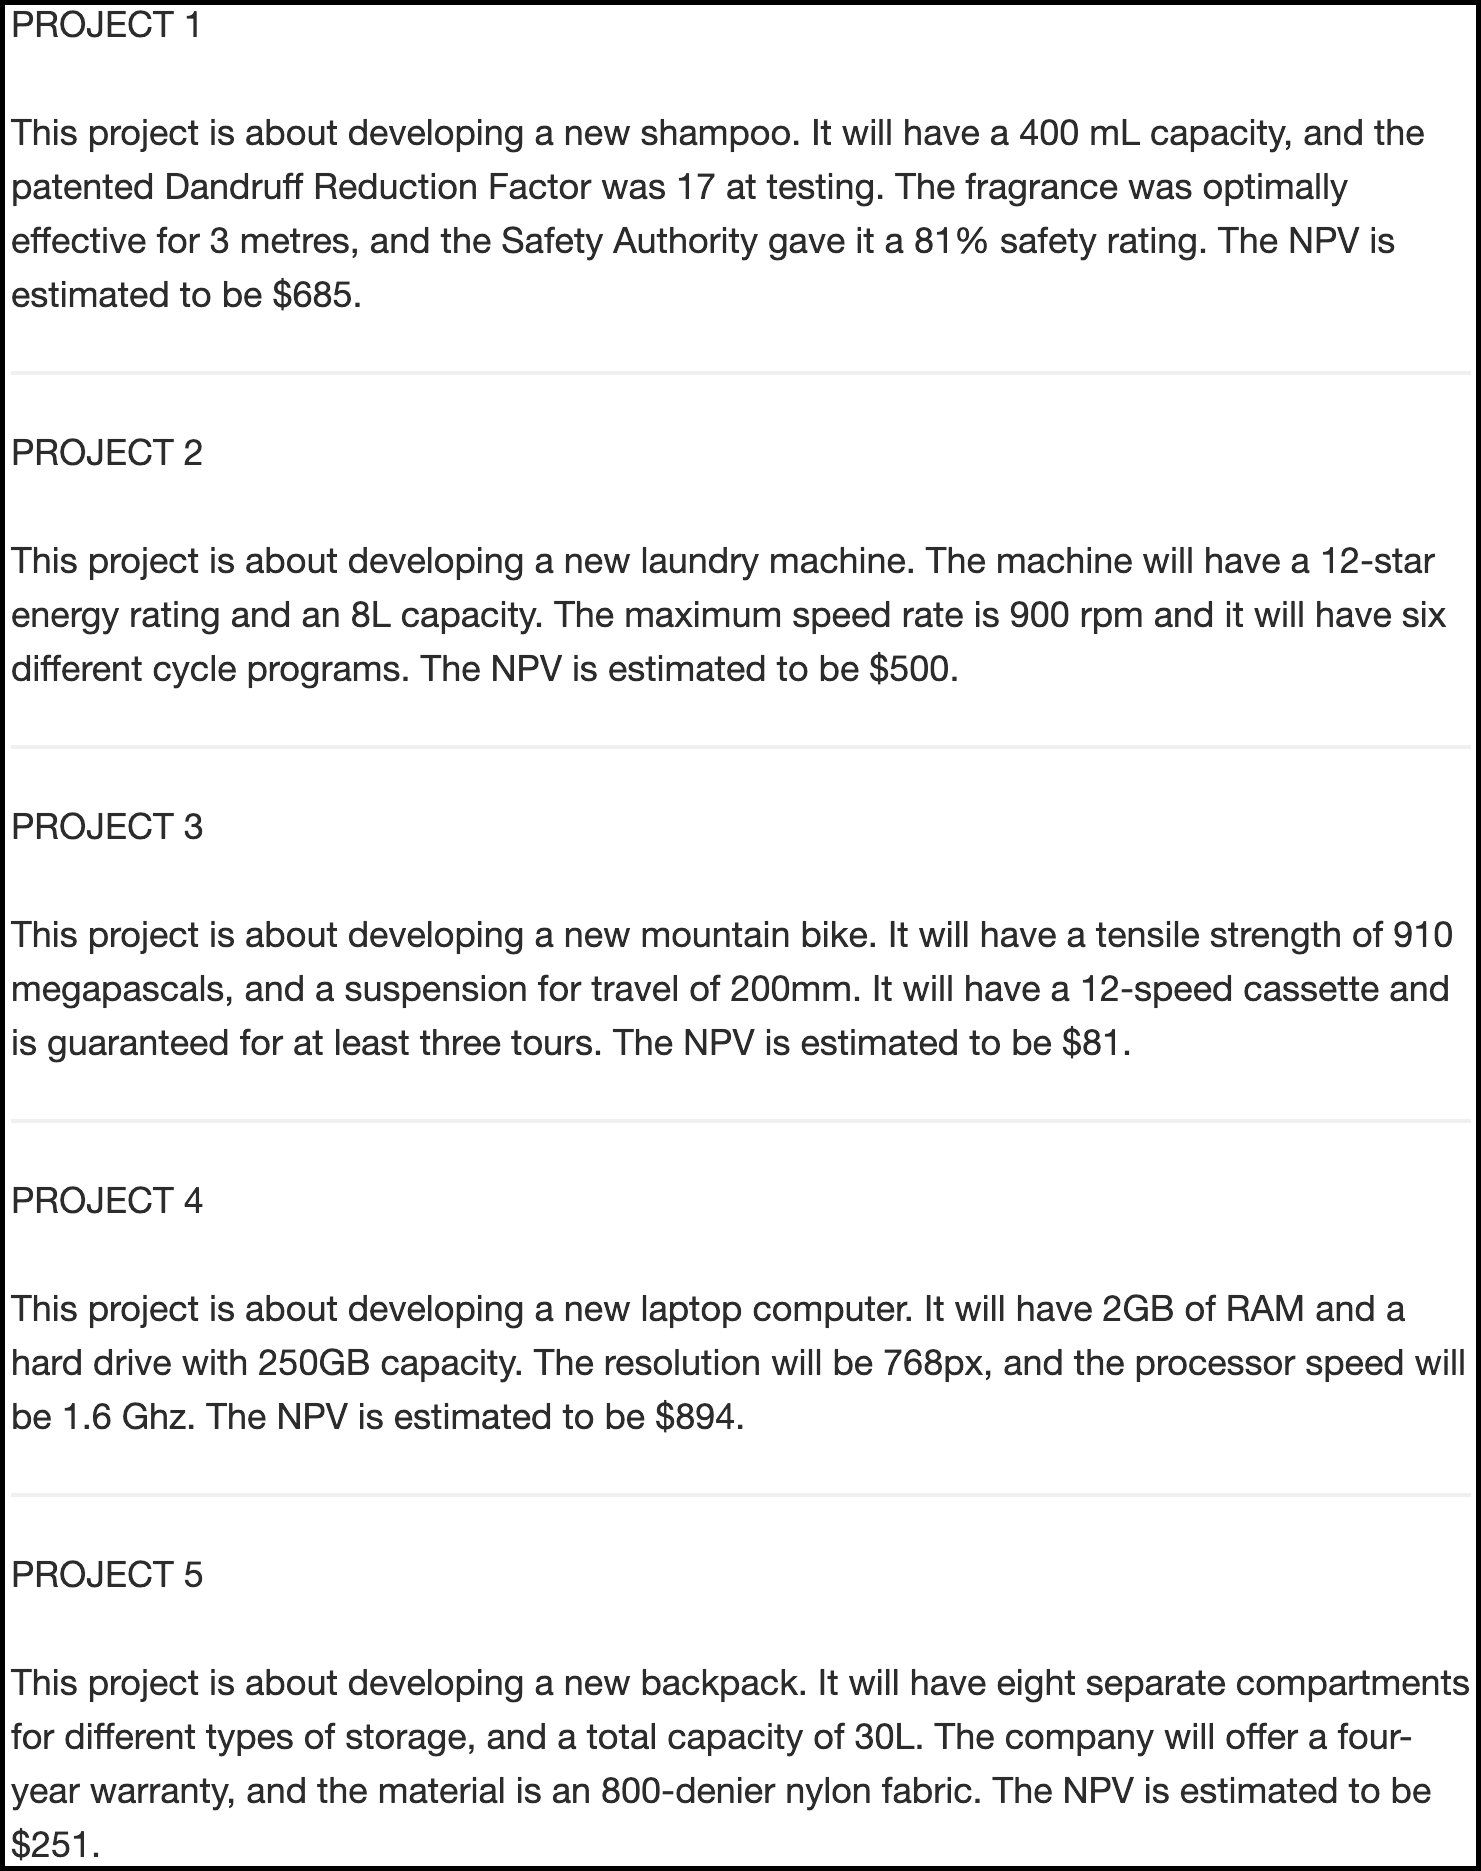
\includegraphics[width=1\linewidth]{thesis_files/figure-latex/projects-alignment-low-materials-alignment-2-1} \caption{An example of a low alignment display in Experiment 1. Border added for clarity.}\label{fig:projects-alignment-low-materials-alignment-2}
\end{figure}



\begin{figure}
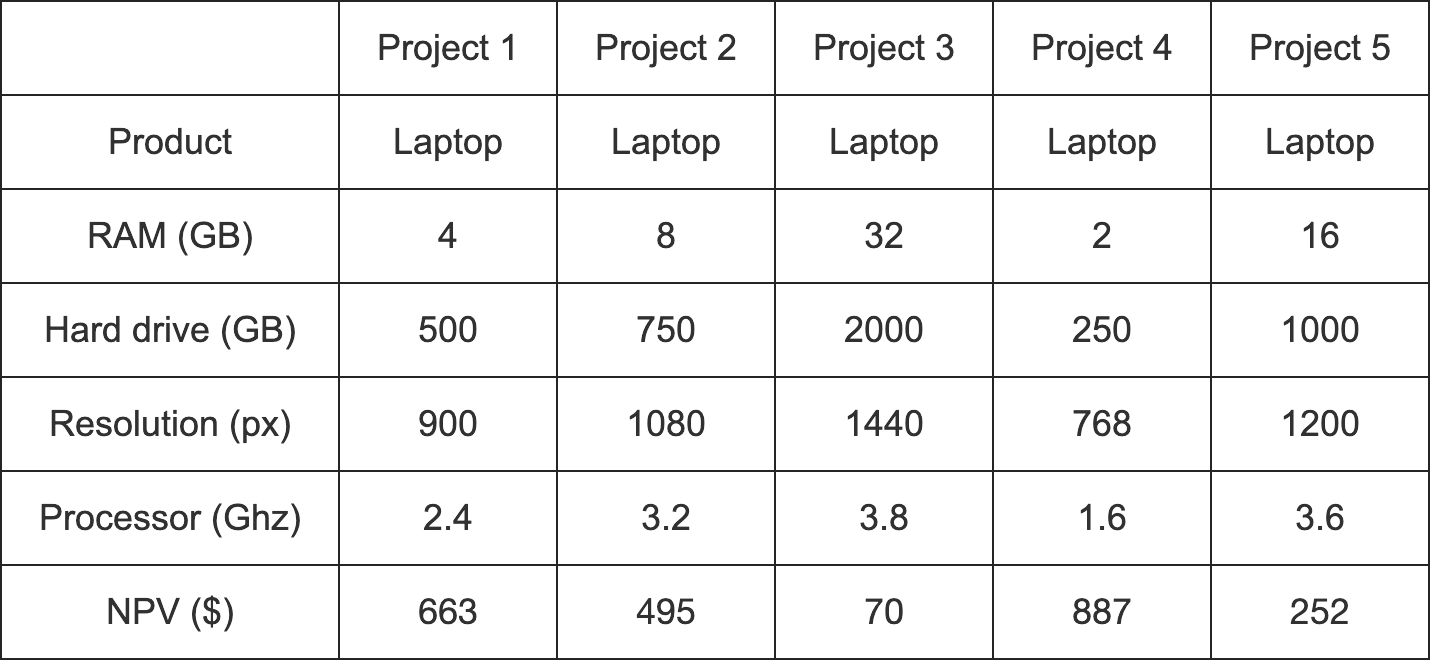
\includegraphics[width=1\linewidth]{thesis_files/figure-latex/projects-alignment-high-materials-alignment-2-1} \caption{An example of a high alignment display in Experiment 1.}\label{fig:projects-alignment-high-materials-alignment-2}
\end{figure}

Critically, the value of the concrete attributes were always in conflict with
the NPV. For instance, Project 4 always had the lowest value for each of the
concrete attributes for laptops, but always had the highest NPV. This was done
in order to be able to use participants' allocations as a proxy measure for an
individual's degree of dependence on NPV.

\hypertarget{allocation}{%
\paragraph{Allocation}\label{allocation}}

Participants completed a resource allocation task (see
Figure~\ref{fig:allocation-alignment-2}), adapted from \textcite{bardolet2011} in which
they were asked to allocate their hypothetical yearly budget across the given
five projects.



\begin{figure}
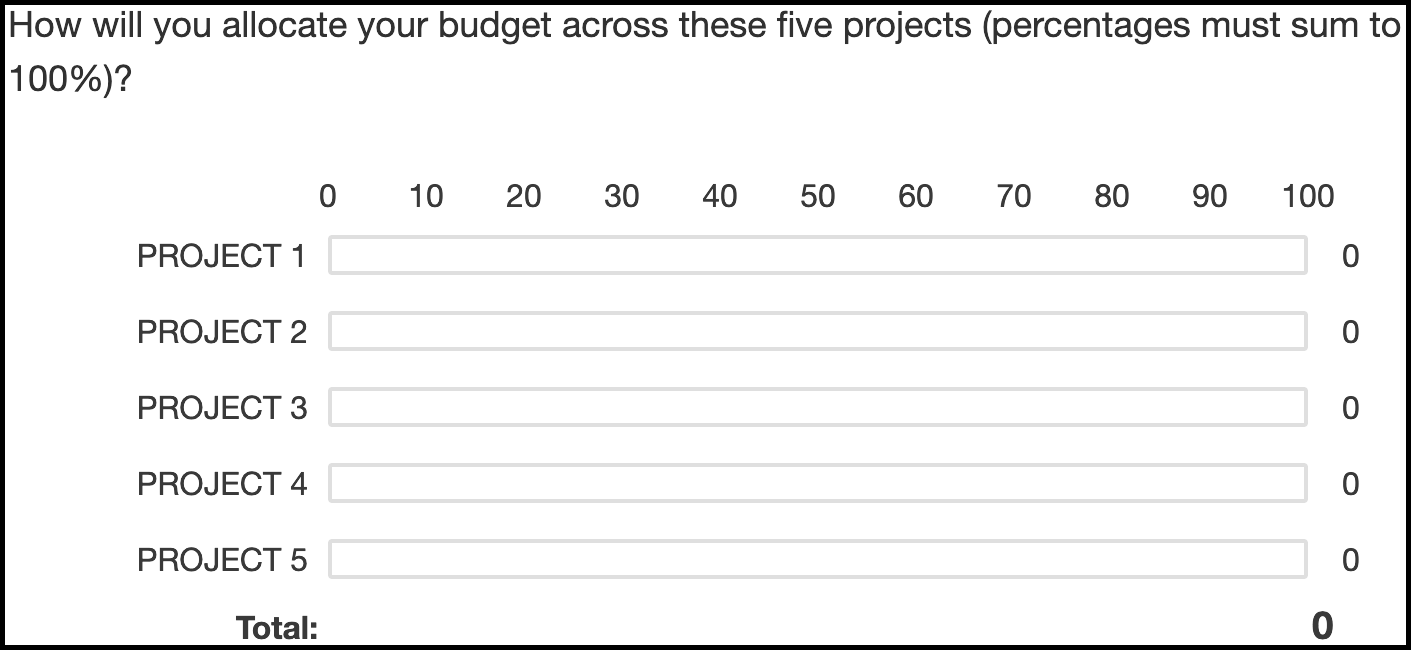
\includegraphics[width=1\linewidth]{thesis_files/figure-latex/allocation-alignment-2-1} \caption{The allocation task.}\label{fig:allocation-alignment-2}
\end{figure}

\hypertarget{additional-measures}{%
\paragraph{Additional measures}\label{additional-measures}}

As well as measuring allocation, I included other measures, whose presentation
and analyses are reported in the Appendix. Specifically, participants were asked
to forecast the future returns of the projects (see
Appendix~\ref{forecasting-materials-alignment-2}), rank the projects (see
Appendix~\ref{ranking-materials-alignment-2}), indicate their confidence in
their decisions (see Appendix~\ref{confidence-materials-alignment-2}), and
justify their decisions (see
Appendix~\ref{justification-materials-alignment-2}).

\hypertarget{procedure-2}{%
\subsubsection{Procedure}\label{procedure-2}}

Following ethics and demographics web-pages, participants were introduced to the
study and the concept of NPV through the instructions page. They then completed
the forecasting task directly after each project display in the low alignment
condition, and directly under all projects for the high alignment condition.
Participants then ranked the projects, and subsequently answered the allocation,
confidence, and justification questions.

\hypertarget{results}{%
\subsection{Results}\label{results}}

A mixed factorial ANOVA was conducted to investigate the effects of alignment
and verbally-instructed NPV reliability on participants' allocations. As seen in
Figure~\ref{fig:plot-alignment-2-allocation}, the alignment \(\times\)
reliability amount \(\times\) NPV amount interaction was significant,
\(F(6.57, 367.76) = 2.18\), \(p = .039\), \(\hat{\eta}^2_p = .038\). This
effect seems to be driven by the differences between the no NPV condition and
the conditions with NPV across the two alignment conditions. Specifically, in
the low alignment condition, the linear NPV trend was significantly lower in the
no NPV condition than both the low reliability condition,
\(M = 64.63\), 95\% CI \([25.76,~103.50]\), \(t(112) = 3.29\), \(p = .001\), and the high
reliability condition, \(M = 60.29\), 95\% CI \([24.14,~96.43]\), \(t(112) = 3.30\), \(p = .001\).
However, in the high alignment condition, the linear NPV trend was only
significantly lower in the no NPV condition than the high reliability condition,
\(M = 75.70\), 95\% CI \([39.17,~112.24]\), \(t(112) = 4.11\), \(p < .001\), and not the low
reliability condition, \(M = 12.24\), 95\% CI \([-27.94,~52.41]\), \(t(112) = 0.60\), \(p = .547\).



\begin{figure}
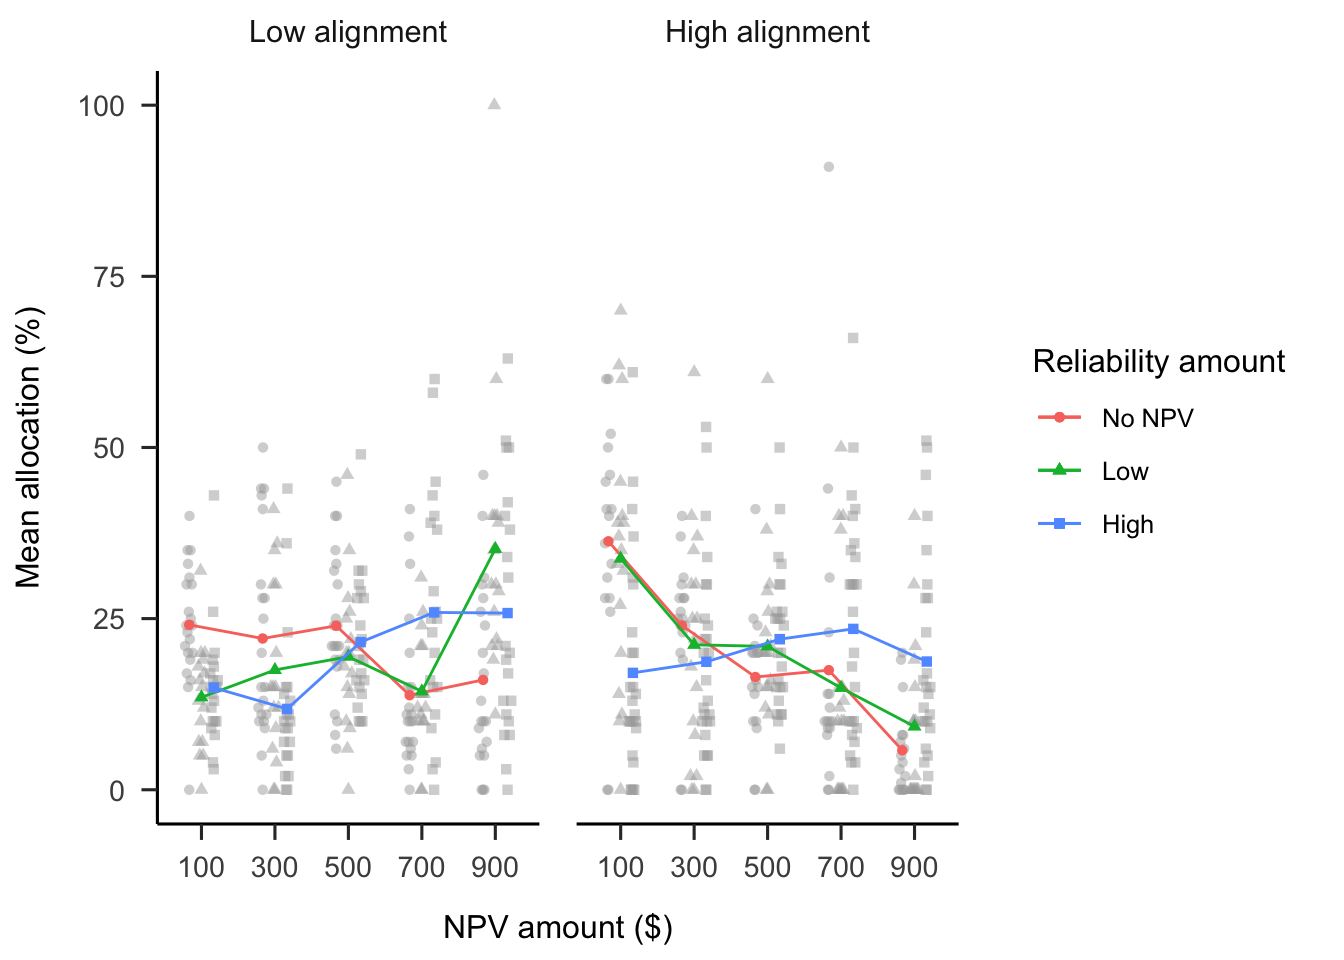
\includegraphics[width=1\linewidth]{thesis_files/figure-latex/plot-alignment-2-allocation-1} \caption{Mean allocation.}\label{fig:plot-alignment-2-allocation}
\end{figure}

The ranking, confidence, and forecast mean data were all largely congruent with
the allocation findings (see Appendix~\ref{results-alignment-2-appendix}). I
also found that the forecasts of those in the low alignment condition had higher
standard deviations than those in the high alignment condition (see
Appendix~\ref{forecast-sd-alignment-2}). However, this did not replicate in
subsequent experiments (see Appendix~\ref{forecast-sd-alignment-4}
and~\ref{forecast-sd-alignment-5}).

\hypertarget{discussion-1}{%
\subsection{Discussion}\label{discussion-1}}

Experiment 1 found evidence for the effect of alignment on laypeople's
decision-making in resource allocation scenarios. Specifically, I found that
when projects are comparable, people use NPV when they are told it is reliable,
but not when they are told it is unreliable. However, they use NPV regardless of
reliability when it is the only shared dimension across products.

In Experiment 1 I manipulated \emph{verbal} NPV reliability. That is, participants
were explicitly told whether NPV is considered to be a reliable metric or not.
However, in the real-world the reliability of a metric is more commonly
expressed in numerical form, such as a range around and estimate. In Experiment
2 I will attempt to replicate the alignment effects, but while manipulating the
numerical reliability associated with each project, rather than the verbal
reliability as I have previously used. Further, it might be the case that only
those with sufficient experience with financial theory and analysis will be able
to successfully draw inferences from such information. Therefore, in Experiment
2 I used a sample of Masters of Management students, instead of the laypeople in
Experiment 1.

\hypertarget{alignment-3}{%
\section{Experiment 2}\label{alignment-3}}

Experiment 2 further investigated the effects of alignment and
numerically-expressed variance information on financial resource allocation
decisions. In \protect\hyperlink{alignment-2}{Experiment 1} the information about the variance
inherent in the NPVs was communicated explicitly as the conclusion, e.g., NPV is
unreliable. In Experiment 2 however, only the actual variance information itself
was communicated without the conclusion about its reliability. Here, I simply
communicated variance by showing the range of predicted values (akin to a
confidence interval). Therefore, while previously I manipulated \emph{verbal}
reliability, in Experiment 2 I manipulated \emph{numerical} reliability. Further, in
this experiment, I studied participants with more business experience than the
previously used laypeople samples. The main two interests in this experiment
were first, whether the previous findings of an alignment effect will replicate
with people with more business experience; and second, whether this population
is sensitive to variance in forecasts. As well as again testing
Hypothesis~\ref{hyp:allocation-alignment-alignment-2}, I tested the following
hypothesis:

\begin{hypothesis}
\protect\hypertarget{hyp:allocation-npv-reliability-alignment-3}{}{\label{hyp:allocation-npv-reliability-alignment-3} }The NPV amount \(\times\) reliability amount interaction will not be significant
in either alignment condition.
\end{hypothesis}

I was also interested in the potential to quickly change participants'
understanding, if they did not initially use numerical reliability for their
allocations. Therefore, I presented participants with a short lecture on the
importance of paying attention variance in financial decision-making. However,
results were inconclusive, so see but see
Appendix~\ref{discussion-alignment-3}, for a more detailed discussion.

\hypertarget{method-3}{%
\subsection{Method}\label{method-3}}

\hypertarget{participants-3}{%
\subsubsection{Participants}\label{participants-3}}

Fifty-four (28 female) people were recruited from a Masters of Management course at an Australian university. Age information was not recorded.~Both the reliability amount conditions (low and
high) and alignment conditions (low and high) were presented within subjects and
their order of presentation was counterbalanced.

\hypertarget{materials-2}{%
\subsubsection{Materials}\label{materials-2}}

\hypertarget{instructions-1}{%
\paragraph{Instructions}\label{instructions-1}}

Participants were shown similar instructions to \protect\hyperlink{instructions-materials-alignment-2}{Experiment
1}. However, here they were given more
information about NPV (about the discount rate and initial investment). See
Appendix~\ref{instructions-materials-alignment-3-appendix} for screenshots of
the instructions.

\hypertarget{npv-test}{%
\paragraph{NPV test}\label{npv-test}}

Participants were presented with a short and simple test of their understanding
of NPV (see Appendix~\ref{npv-test-materials-alignment-3}).

\hypertarget{project-display}{%
\paragraph{Project display}\label{project-display}}

As seen in Figures~\ref{fig:projects-alignment-low-materials-alignment-3}
and~\ref{fig:projects-alignment-high-materials-alignment-3}, the project
display was as in \protect\hyperlink{projects-materials-alignment-2}{Experiment 1}, except for
the addition of another set of projects that differed in semantic content. That
is, the projects were about different types of projects (to allow for a
within-subjects manipulation). Along with the single NPV, the forecasted ranges
of cash flow that the NPV was calculated from were presented. In the low
numerical reliability condition, the ranges were \(\pm85\)\% around the mean (e.g.,
\$150-\$1850, where the forecast mean is \$1000); whereas in the high numerical
reliability condition, the ranges were \(\pm5\)\% around the mean (e.g.,
\$950-\$1050, where the forecast mean is \$1000). Wide ranges should indicate low
reliability in the measure, while narrow ranges should indicate high
reliability. Between the four displays, participants were told to treat each new
set of projects as independent to the other sets.



\begin{figure}
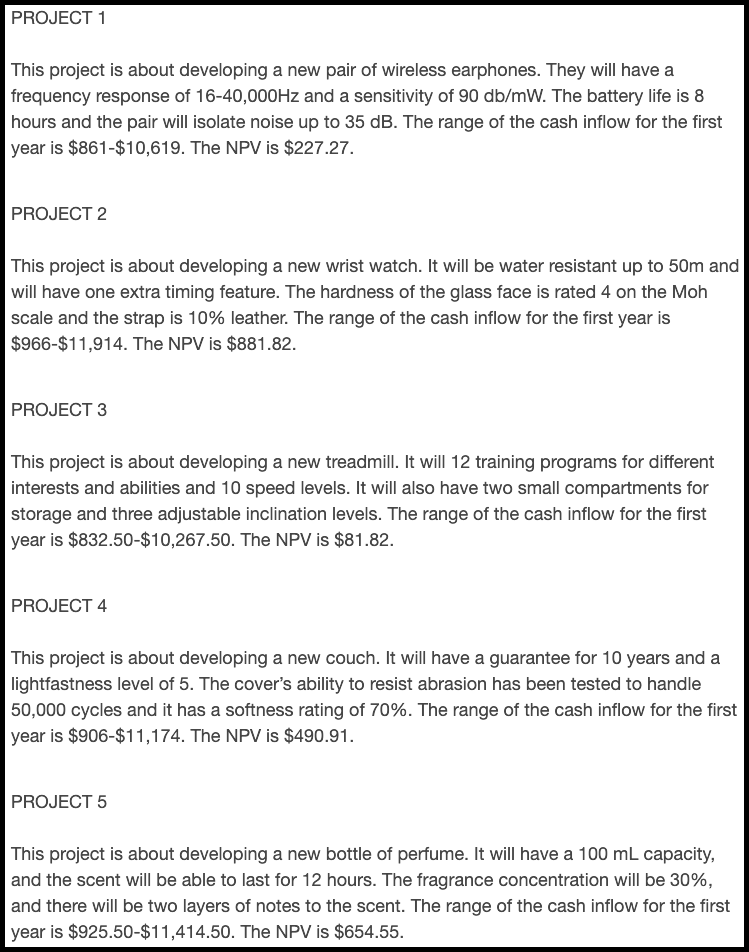
\includegraphics[width=1\linewidth]{thesis_files/figure-latex/projects-alignment-low-materials-alignment-3-1} \caption{An example of a low alignment low reliability display in Experiment 2. Border added for clarity.}\label{fig:projects-alignment-low-materials-alignment-3}
\end{figure}



\begin{figure}
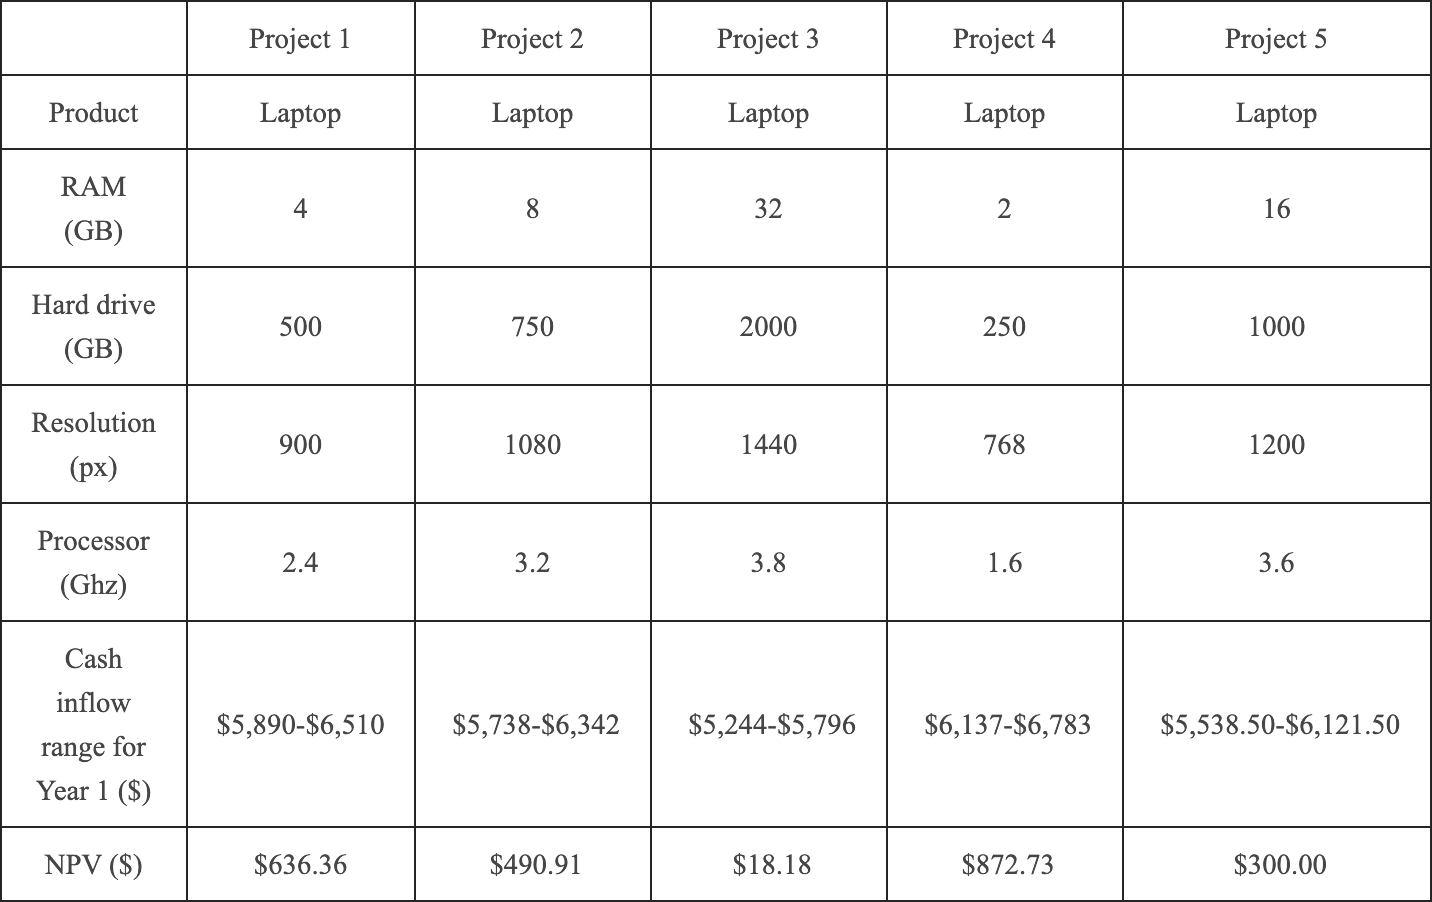
\includegraphics[width=1\linewidth]{thesis_files/figure-latex/projects-alignment-high-materials-alignment-3-1} \caption{An example of a high alignment high reliability display in Experiment 2.}\label{fig:projects-alignment-high-materials-alignment-3}
\end{figure}

\hypertarget{npv-knowledge-ratings}{%
\paragraph{NPV knowledge ratings}\label{npv-knowledge-ratings}}

I was interested if the participants would be overconfident in their knowledge
of NPV, so asked them to rate this at multiple points in the experiment (see
Appendix~\ref{npv-knowledge-materials-alignment-3}).

\hypertarget{variance-lecture}{%
\paragraph{Variance lecture}\label{variance-lecture}}

Participants were shown a short lecture on the importance of paying attention to
variance information, in an attempt to facilitate a subsequent increased use of
the numerical reliability information in their allocations (see
Appendix~\ref{variance-lecture-materials-alignment-3} for more details and the
lecture slides).

\hypertarget{procedure-alignment-3}{%
\subsubsection{Procedure}\label{procedure-alignment-3}}

Participants saw the instructions, NPV explanation, and completed a simple test
to demonstrate their understanding of NPV. They then completed four
counterbalanced resource allocation trials (equivalent to each condition
combination), and saw a brief presentation about the importance of paying
attention to variance in financial decision-making. Subsequently, participants
completed a further two resource allocation trials, of two of the trials that
they subsequently saw earlier. They were shown the allocations they provided
earlier, and given the opportunity to change them. With the knowledge ratings,
participants rated once before the NPV test, re-rated after the test, and after
the four project displays. They were then asked to rate their knowledge of NPV
as they believe it had been both before and after the variance presentation.

\hypertarget{results-1}{%
\subsection{Results}\label{results-1}}

A mixed factorial ANOVA was conducted to investigate the effects of NPV amount,
alignment, and numerical NPV reliability on participants' project allocations.
Figure~\ref{fig:plot-alignment-3-allocation} shows these data. The alignment
\(\times\) reliability amount \(\times\) NPV amount interaction was
significant,
\(F(2.81, 148.75) = 3.95\), \(p = .011\), \(\hat{\eta}^2_p = .069\),
however, this appeared to be driven by the difference between alignment
conditions in the interaction between the quadratic NPV amount trend and
reliability amount,
\(\Delta M = -42.28\), 95\% CI \([-76.96,~-7.59]\), \(t(53) = -3.14\), \(p = .011\), even after
applying a Šidák correction. The same interaction but with the linear NPV trend
was not significant,
\(\Delta M = -6.13\), 95\% CI \([-31.50,~19.25]\), \(t(53) = -0.62\), \(p = .954\). Further, the linear
NPV trend did not differ between reliability amount condition in neither the low
alignment condition, \(\Delta M = -3.19\), 95\% CI \([-18.77,~12.40]\), \(t(53) = -0.41\), \(p = .683\), nor
the high alignment condition,
\(\Delta M = 2.94\), 95\% CI \([-12.63,~18.52]\), \(t(53) = 0.38\), \(p = .706\). However, averaging over
reliability amount, the linear NPV trend was higher in the low alignment
condition than in the high alignment condition,
\(\Delta M = 28.19\), 95\% CI \([5.57,~50.81]\), \(t(53) = 2.50\), \(p = .016\).



\begin{figure}
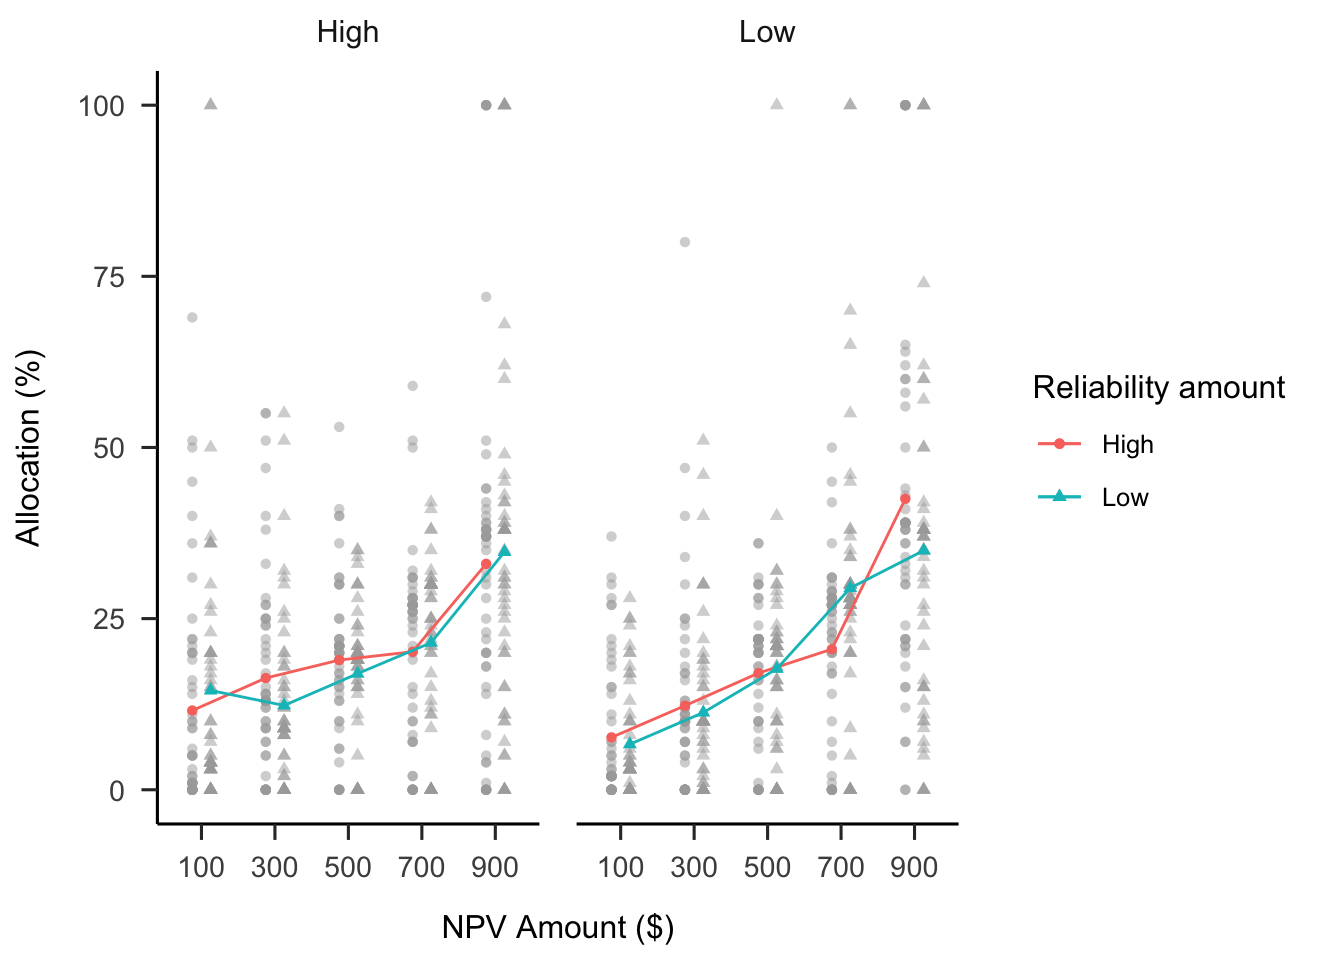
\includegraphics[width=1\linewidth]{thesis_files/figure-latex/plot-alignment-3-allocation-1} \caption{Mean allocation.}\label{fig:plot-alignment-3-allocation}
\end{figure}

The ranking data were congruent with these results, while the confidence data
was less so. Further, the NPV knowledge data did not replicate the effect from
\textcite[Study 1]{long2018}. These analyses are reported in
Appendix~\ref{results-alignment-3-appendix}.

\hypertarget{discussion-2}{%
\subsection{Discussion}\label{discussion-2}}

Experiment 2 replicated the alignment effect found in Experiment 1 with
participants with real-world business experience. I found evidence for
Hypothesis~\ref{hyp:allocation-alignment-alignment-2}, as people seemed to rely
more on NPV when faced with a set of dissimilar project than when projects were
all from the same domain. Further, I found evidence for
Hypothesis~\ref{hyp:allocation-npv-reliability-alignment-3}, with no
significant differences between the numerical reliability amount conditions.
While I did not replicate the interaction found in Experiment 1, it should be
emphasised that these are two different effects. In Experiment 1, I explicitly
told participants about the reliability of the NPV measure, whereas in
Experiment 2, I provided them with variance information that merely implies NPV
reliability. Thus, I showed that business students are affected by comparability
of project sets, but not by numerical NPV reliability information. Specifically,
participants appeared to only focus on the NPV itself, and not on any variations
in the underlying noisiness of the measure for a specific project.

However, it is unclear whether laypeople would also display this variance
neglect. Further, in Experiments 1 and 2, the business projects consisted of
a limited number of domains. It is unclear to what extent these specific domains
influenced the results. These projects were centred around consumer products,
with various features displayed. Consumer projects were chosen to be more easily
accessible to participants without business experience. However, with these
projects, individual features do not necessarily indicate a project's
profitability. For instance, a laptop with a low capacity can be more profitable
than a laptop with a high capacity due to the existence of consumer goods
markets. In Experiment 3, I addressed these limitations.

Another limitation of the last two experiments was the potential presentation
style confound. The two alignment conditions differed in the number of alignable
differences, but also in the way that the information was presented. The
information in the low alignment condition was presented in paragraphs, whereas
the information in the high alignment condition was presented in tables. While
it is likely that each of these data types would be presented in this way in a
business setting, it is important to rule out that this manipulation did not
also unnecessarily increase task difficulty. Therefore, Experiment 3 attempted
to replicate this effect, while controlling for presentation style.

\hypertarget{experiment-3}{%
\section{Experiment 3}\label{experiment-3}}

Experiment 3 investigated the effects of alignment, reliability type, NPV
amount, and reliability amount on allocations. Experiment 1 manipulated
reliability amount by using \emph{verbal} prompts. That is, participants were told
explicitly whether or not NPV was reliable for a certain project industry.
Experiment 2 investigated whether people were able to extract this same kind of
reliability information from \emph{numerical} prompts. That is, participants saw NPVs
with either wide or narrow ranges, indicating either low or high reliability of
the metric, respectively. However, Experiment 1 sampled laypeople, whereas
Experiment 2 sampled a Masters of Management course. Therefore, I was not able
to compare the two reliability types (verbal and numerical) without ruling out
the potential confound of population type. As such, in Experiment 3 I
manipulated NPV amount, alignment, and reliability amount, but also added a
reliability type factor. Further, presentation style was a possible confound in
the alignment manipulation of the previous experiments. That is, the business
projects in the high alignment condition were always displayed as a part of a
table, whereas the projects in the low alignment condition were displayed in
prose, as paragraphs. Experiment 3 fixed this by using the same presentation
style across alignment condition.

As well as again testing
Hypotheses~\ref{hyp:allocation-alignment-alignment-2},~\ref{hyp:allocation-alignment-reliability-npv-alignment-2},~\ref{hyp:allocation-alignment-high-alignment-2},
and~\ref{hyp:allocation-alignment-low-alignment-2}, I tested the following
hypothesis (see Figure~\ref{fig:plot-simulation-alignment-8} for a plot of a
simulation of all hypothesised effects):

\begin{hypothesis}
\protect\hypertarget{hyp:four-way-alignment-8}{}{\label{hyp:four-way-alignment-8} }The alignment \(\times\) reliability amount \(\times\) reliability type \(\times\) NPV
amount interaction will be significant, such that the effects hypthesised above
will be seen in the verbal reliability condition, but none of these effects
will be seen in the numerical reliability condition.
\end{hypothesis}

\hypertarget{method-4}{%
\subsection{Method}\label{method-4}}

\hypertarget{participants-4}{%
\subsubsection{Participants}\label{participants-4}}

Four hundred and forty-eight (176 female) people were recruited from the online recruitment platform Prolific. Participants were compensated at a rate of £5 an hour. The average age was 41.65 (\emph{SD} = 10.3, \emph{min} = 29, \emph{max} = 78). Participants reported an average of 6.94 (\emph{SD} = 8.23, \emph{min} = 0, \emph{max} = 43) years of work in a business setting, and an average of 3.73 (\emph{SD} = 6.27, \emph{min} = 0, \emph{max} = 45) years of business education. The mean completion time was 11.35 (\emph{SD} = 10.79, \emph{min} = 1.92, \emph{max} = 183.7) minutes.~Table~\ref{tab:condition-allocation-alignment-8}
shows the between-subjects condition allocation. The two reliability amount
conditions (low and high) were presented within subjects and the order of their
presentation was randomised. As before, NPV amount was varied within subjects.
Therefore, each participant saw two separate project displays.
Appendix~\ref{power-analysis-alignment-8} describes the power analysis
conducted to arrive at this sample size.

\begin{table}[tbp]

\begin{center}
\begin{threeparttable}

\caption{\label{tab:condition-allocation-alignment-8}Experiment 3 group allocation.}

\begin{tabular}{lll}
\toprule
Alignment & \multicolumn{1}{c}{Reliability type} & \multicolumn{1}{c}{N}\\
\midrule
High & Explicit & 112\\
High & Implicit & 112\\
Low & Explicit & 112\\
Low & Implicit & 112\\
Total & - & 448\\
\bottomrule
\end{tabular}

\end{threeparttable}
\end{center}

\end{table}

\hypertarget{materials-3}{%
\subsubsection{Materials}\label{materials-3}}

\hypertarget{instructions-2}{%
\paragraph{Instructions}\label{instructions-2}}

Participants saw similar instructions to the previous experiments, with an added
explanation of the NPV reliability information for each reliability type
condition (see Appendix~\ref{instructions-materials-alignment-8-appendix}). Further, they
completed a test of basic NPV understanding. This test was added also as an
attention check as, although it was required to answer, the response should only
be one of two letters.

\hypertarget{project-display-1}{%
\paragraph{Project display}\label{project-display-1}}

The project displays were similar to the previous experiments. However, here
participants saw the same presentation style in both alignment conditions. Each
display had a table describing the projects in the set, with ranking and
allocation inputs. The project details were presented as dot points within the
relevant cells of the table.
Figure~\ref{fig:projects-alignment-low-reliability-explicit-low-materials-alignment-8}
shows an example of a low alignment, low verbal reliability display and
Figure~\ref{fig:projects-alignment-high-reliability-implicit-high-materials-alignment-8}
shows an example of a high alignment, high numerical reliability display.



\begin{figure}
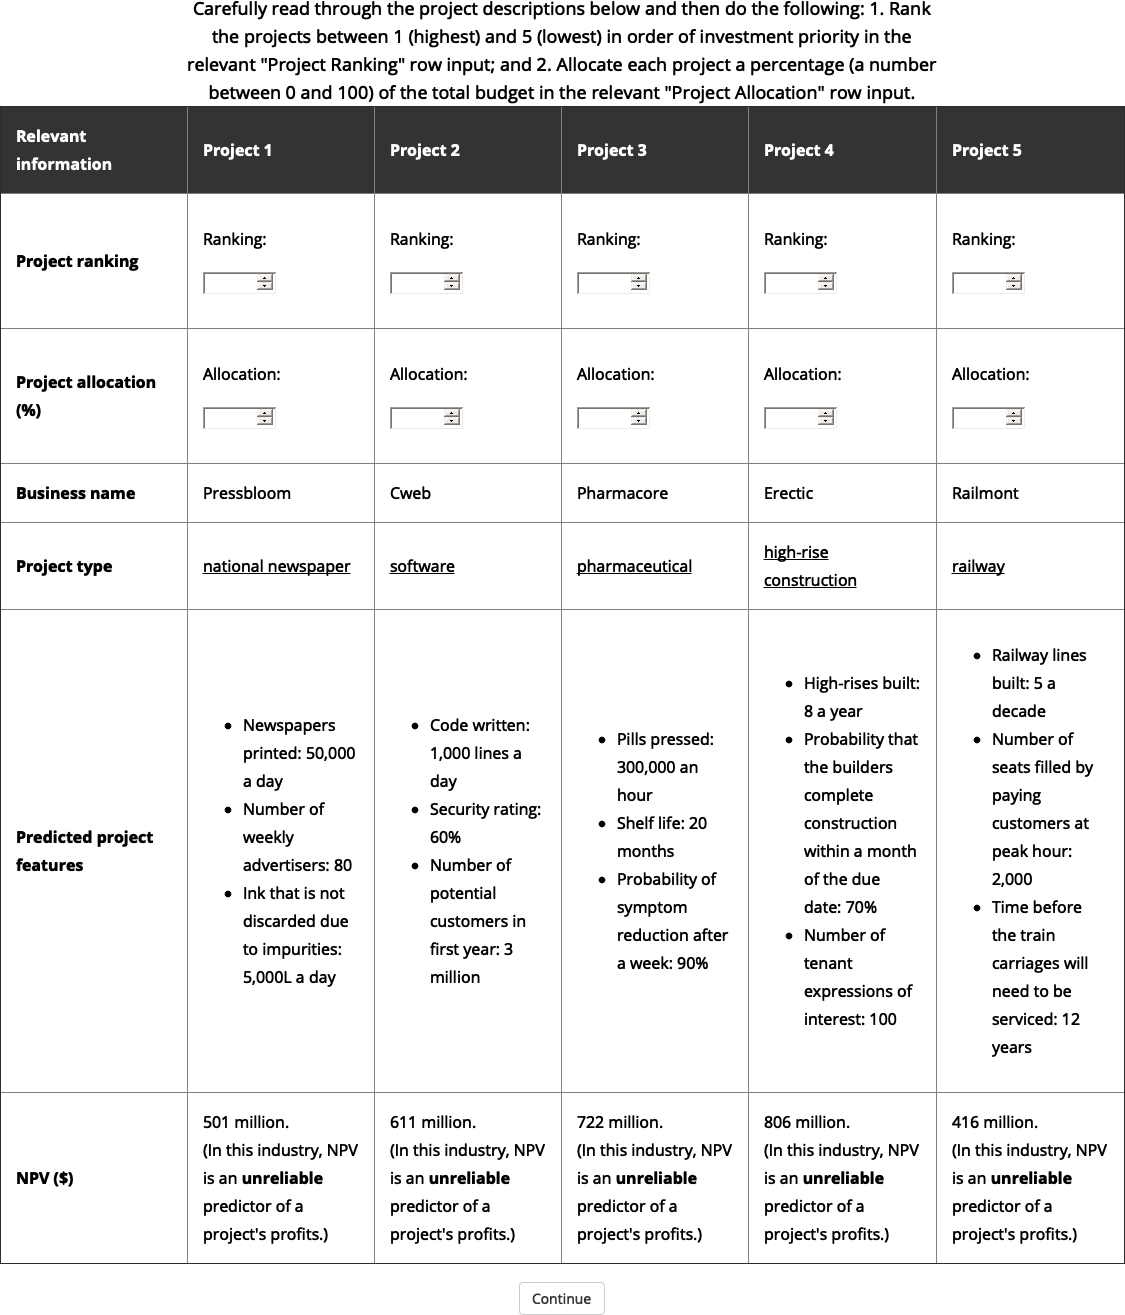
\includegraphics[width=1\linewidth]{thesis_files/figure-latex/projects-alignment-low-reliability-explicit-low-materials-alignment-8-1} \caption{An example of a low alignment, low verbal reliability display in Experiment 3.}\label{fig:projects-alignment-low-reliability-explicit-low-materials-alignment-8}
\end{figure}



\begin{figure}
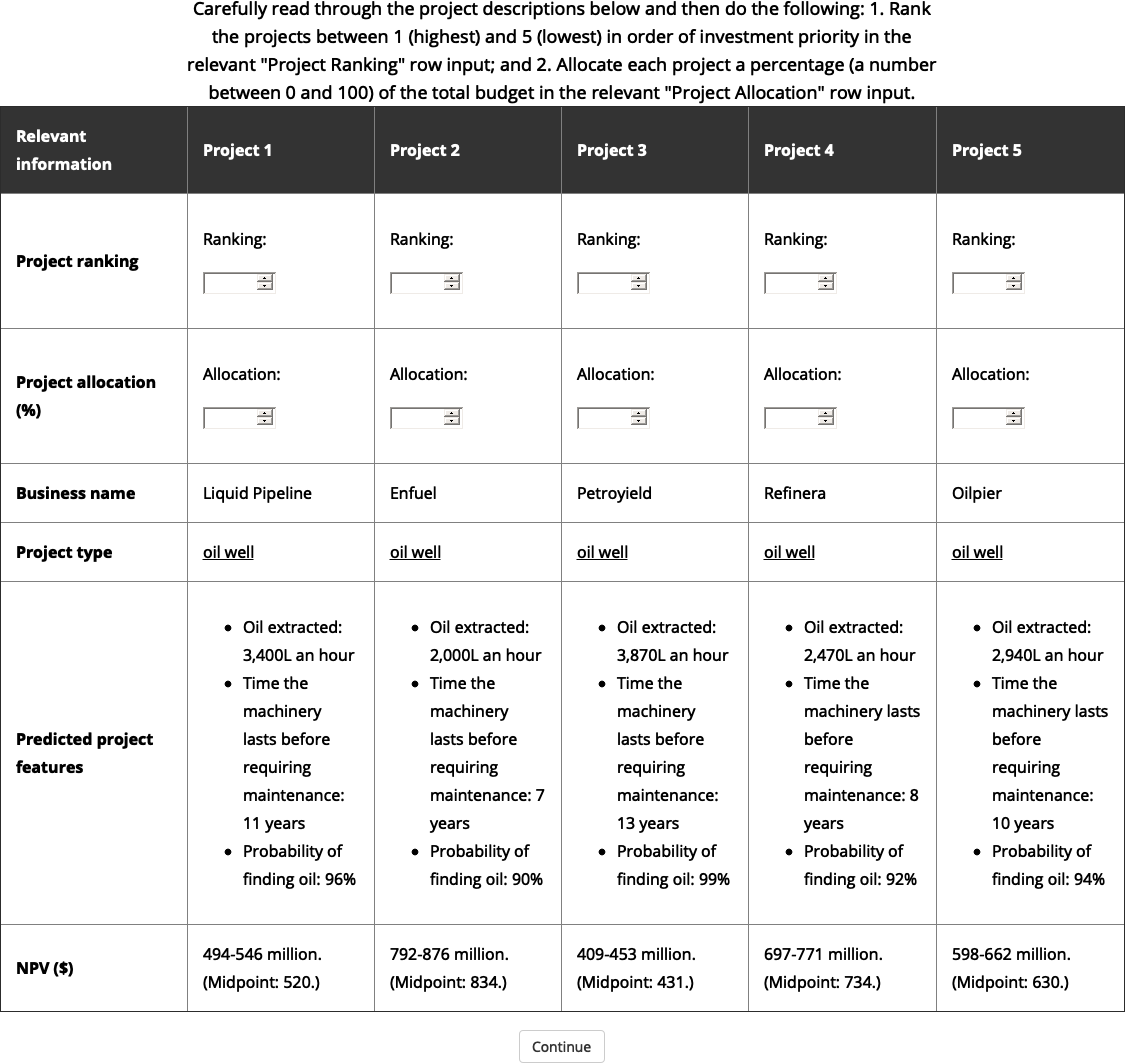
\includegraphics[width=1\linewidth]{thesis_files/figure-latex/projects-alignment-high-reliability-implicit-high-materials-alignment-8-1} \caption{An example of a high alignment, high numerical reliability display in Experiment 3.}\label{fig:projects-alignment-high-reliability-implicit-high-materials-alignment-8}
\end{figure}

Three elements were counterbalanced: 1. the association of reliability amount
and project set (two variations), 2. the association of business name with NPV
(five latin square variations), and 3. project variation (five variations per
alignment condition), which for high alignment meant the project type. For low
alignment this meant the intrinsic feature variant for the relevant project
type. Table column order and project display order were both randomised.

\hypertarget{interstitial}{%
\paragraph{Interstitial}\label{interstitial}}

Before each project display, participants saw an ``interstitial'' page, whose role
was to 1. introduce the next display, and 2. check the participant's attention
(not required to answer, so can be skipped if the interstitial text isn't read).
See Appendix~\ref{interstitial-materials-alignment-8} for an example.

\hypertarget{results-2}{%
\subsection{Results}\label{results-2}}

A mixed factorial ANOVA was conducted to investigate the effects of NPV amount,
alignment, NPV reliability amount, and NPV reliability type on participants'
project allocations. Figure~\ref{fig:plot-alignment-8-allocation} shows these
data. Only the main results are reported here, while the rest of the
hypothesised allocation effects are reported in
Appendix~\ref{results-alignment-8-allocation}.

The four-way interaction (alignment \(\times\) reliability amount \(\times\) NPV
amount \(\times\) reliability type) was not significant,
\(F(3.20, 1,420.19) = 0.71\), \(p = .555\), \(\hat{\eta}^2_p = .002\). Further, the three-way interaction
(alignment \(\times\) reliability amount \(\times\) NPV amount) in the verbal
reliability condition was not significant,
\(\Delta M = 13.42\), 95\% CI \([-1.27,~28.11]\), \(t(444) = 1.80\), \(p = .073\). This is
most likely due to the size of the two-way interactions in each alignment
condition being relatively similar, despite the expectation of no interaction in
the low alignment condition (as was seen in \protect\hyperlink{results-alignment-2}{Experiment
1}). In high alignment, this interaction (between the
linear NPV amount trend and NPV reliability amount) was significant,
\(\Delta M = -36.63\), 95\% CI \([-47.02,~-26.25]\), \(t(444) = -6.93\), \(p < .001\).
Specifically, the trend was stronger in the high reliability amount condition,
\(\Delta M = 27.26\), 95\% CI \([17.69,~36.83]\), \(t(444) = 5.60\), \(p < .001\),
than in the low reliability amount condition,
\(\Delta M = -9.38\), 95\% CI \([-18.86,~0.11]\), \(t(444) = -1.94\), \(p = .053\).
The same interaction was significant in the low alignment condition,
\(\Delta M = -23.21\), 95\% CI \([-33.60,~-12.83]\), \(t(444) = -4.39\), \(p < .001\).
Despite the lack of a three-way interaction in the verbal reliability condition
(indicating a difference in the two alignment two-way interactions), the linear
NPV amount trend was stronger in the low alignment condition than in the high
alignment condition when averaging over reliability amount,
\(\Delta M = 28.97\), 95\% CI \([17.68,~40.26]\), \(t(444) = 5.04\), \(p < .001\).

In the numerical reliability condition, the linear NPV amount trend was not
significantly ``equivalent'' between those in the low and high alignment
conditions (averaging over reliability amount),
\(\Delta M = 15.19\), 95\% CI \([3.90,~26.48]\), \(t(444) = 2.64\), \(p = .996\). In
fact, a post-hoc comparison suggests that the low alignment trend was stronger
(with Bonferroni adjustment),
\(\Delta M = 15.19\), 95\% CI \([0.78,~29.60]\), \(t(444) = 2.64\), \(p = .034\). Further,
the difference between the linear NPV trend was not significantly different
between reliability amount conditions in both the low alignment condition,
\(\Delta M = 1.64\), 95\% CI \([-11.61,~14.90]\), \(t(444) = 0.31\), \(p > .999\),
and high alignment condition,
\(\Delta M = -1.21\), 95\% CI \([-14.46,~12.05]\), \(t(444) = -0.23\), \(p > .999\).
This replicates the finding from \href{results-alignment-3}{Experiment 2} that NPV is
used more in low alignment, but numerical reliability is ignored.



\begin{figure}
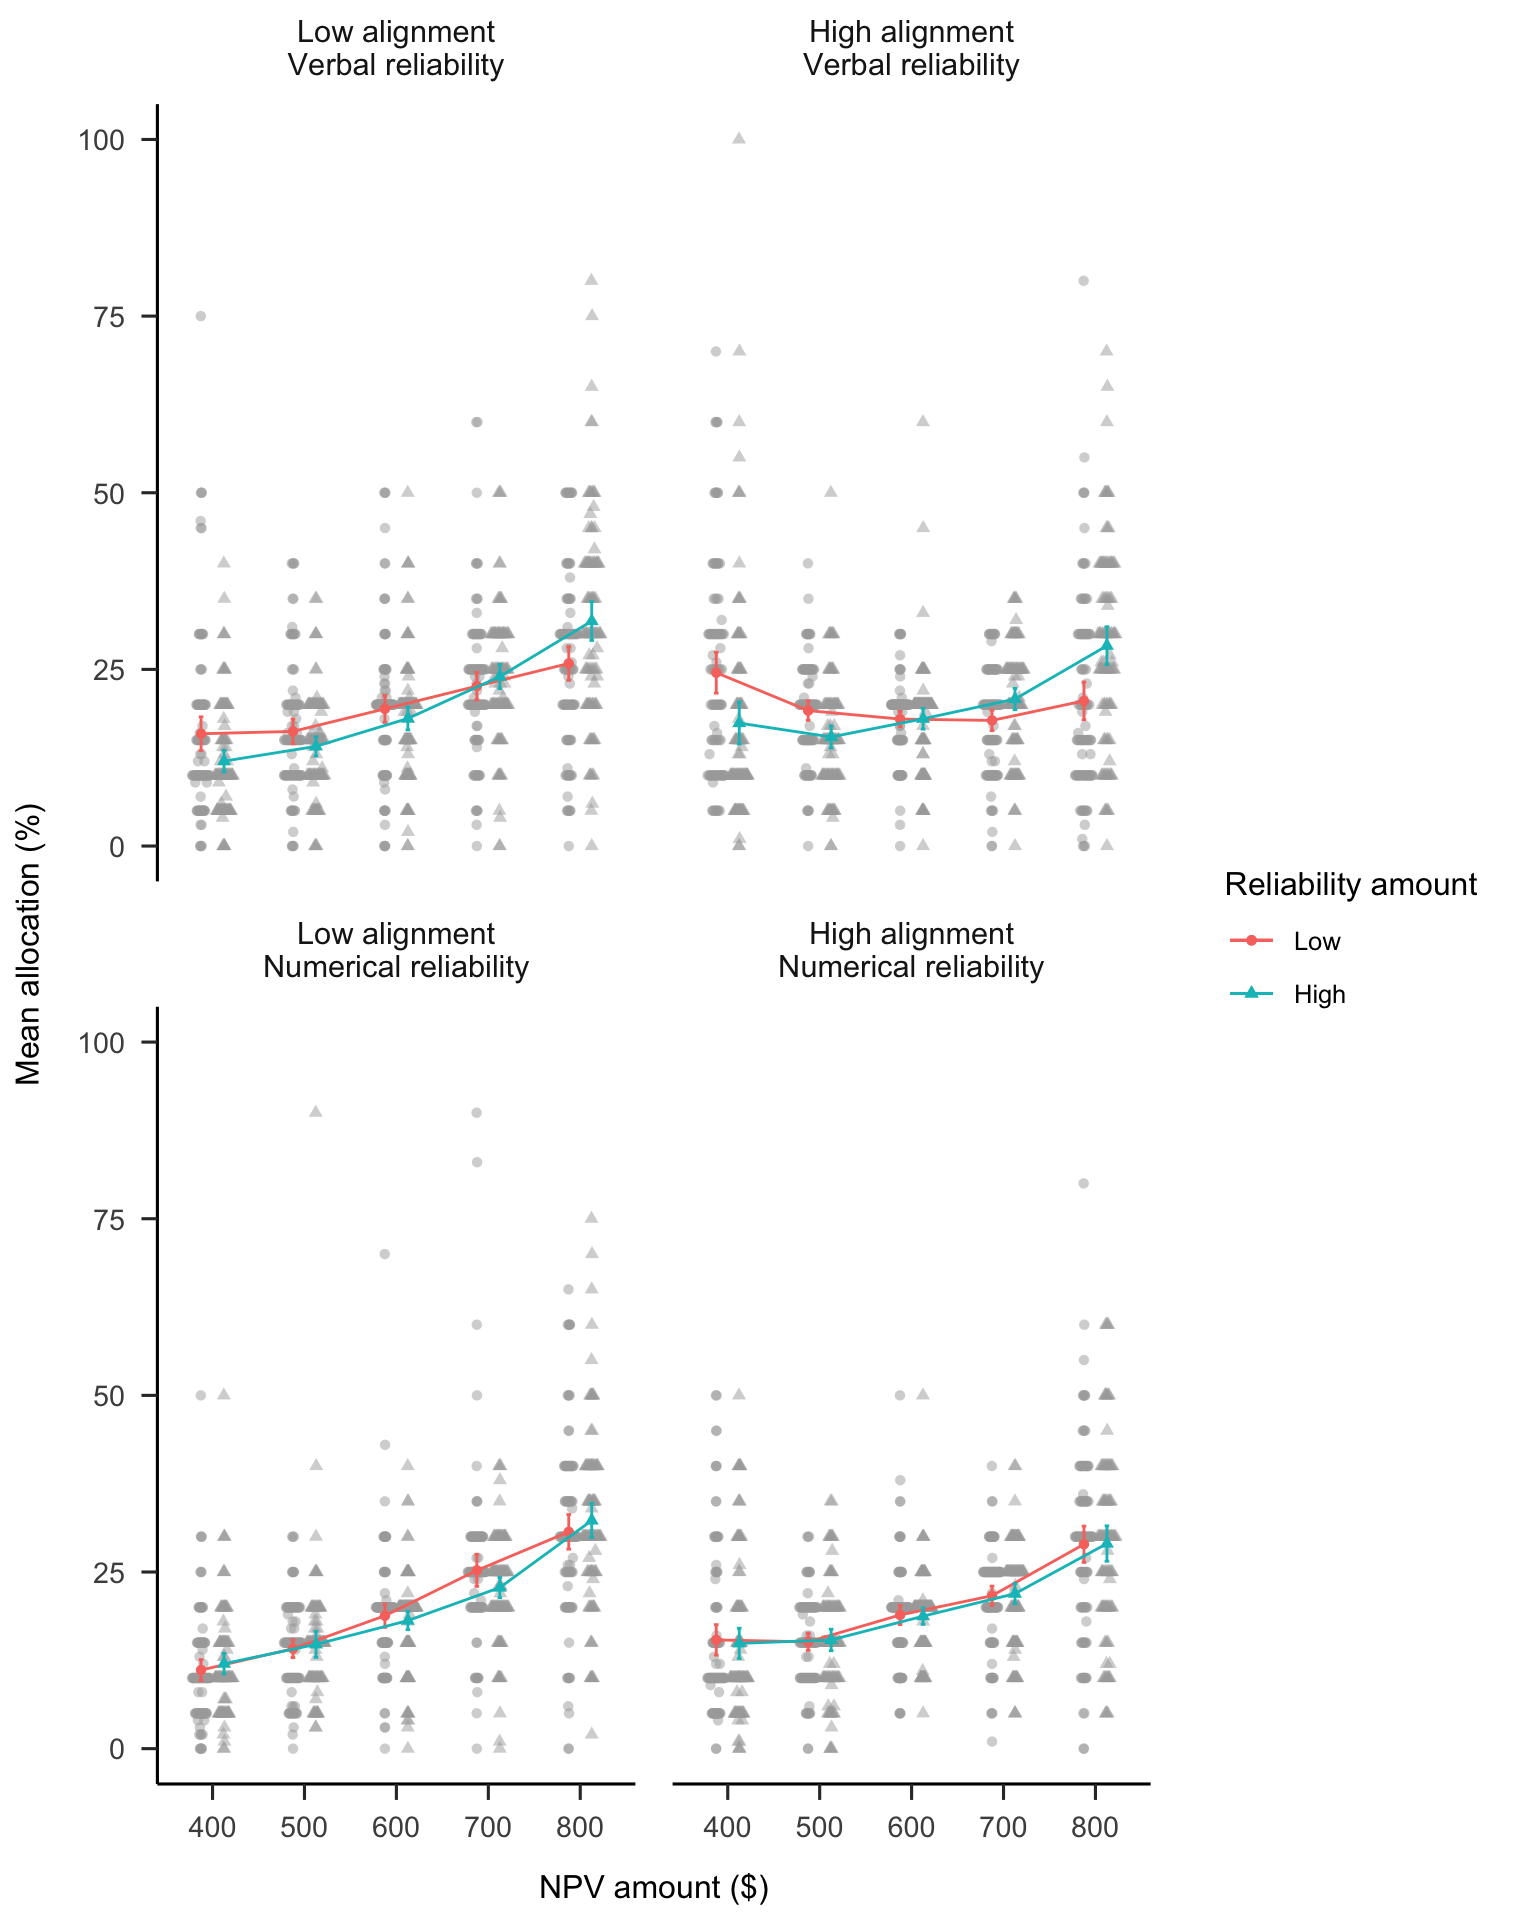
\includegraphics[width=1\linewidth]{thesis_files/figure-latex/plot-alignment-8-allocation-1} \caption{Mean project allocation for all conditions.}\label{fig:plot-alignment-8-allocation}
\end{figure}

\hypertarget{discussion-3}{%
\subsection{Discussion}\label{discussion-3}}

Hypotheses~\ref{hyp:allocation-alignment-alignment-2},~\ref{hyp:allocation-alignment-reliability-npv-alignment-2},
and~\ref{hyp:allocation-alignment-high-alignment-2} were supported. This shows
that while overall participants prefer to use NPV as a proxy for project quality
in their allocations, they still use verbal reliability information.
Specifically, when projects are similar, people use NPV when they are told that
it is reliable, and use alternative metrics when told that it is not reliable.
However, Experiment 3 did not find evidence for
Hypothesis~\ref{hyp:allocation-alignment-low-alignment-2}. Instead, I found
that even in the low alignment condition, participants were still able to use
NPV more when told that it was reliable.

Further, I did not find support for Hypothesis~\ref{hyp:four-way-alignment-8}.
The hypothesis was constructed in response to the results of a pilot study
(documented in Appendix~\ref{alignment-7}) that replicated the results of
Experiment 1 in the verbal reliability condition, but did not replicate the
results of Experiment 2 in the numerical reliability condition. That is, I found
that when faced with numerical ranges as variance information, people did not
seem to even use the midpoint in their decisions. In Experiment 3, on the other
hand, I replicated the finding of Experiment 2 in the numerical reliability
condition. Specifically, I found that people used NPV more when projects were
dissimilar, but critically, that they did not use numerical range information to
moderate their allocations.

\hypertarget{general-discussion-1}{%
\section{General discussion}\label{general-discussion-1}}

Across three experiments there were two main findings: 1. NPV is used more when
options are hard to compare; and 2. people do not consider numerical variance
information, despite this being important to the reliability of the NPV
forecasts. I found these effects consistently across both naive and experienced
populations, which indicates their persistence. When finding themselves in a
situation that requires comparison across disparate options, people make use of
metrics with alignable differences. However, they do not sufficiently moderate
their use of such metrics even when they have alternative attributes to use.

In Experiment 1, I found that when participants were told that NPV was
unreliable, they did not use it in their allocation decisions, but when they
were told that it was reliable they did. In Experiment 2, I found that people
with some business experience relied on NPV more for resource allocation when
the rest of the information was non-alignable, compared to when it was
alignable. However, participants did not take into account the \emph{numerical}
reliability information when making these decisions. In Experiment 3, I found
further evidence of these effects, within one experimental design.

Alignable differences have been shown to be important to decision making in many
settings \autocite{markman2010,markman1995}. The experiments in this chapter are novel
in the investigation of alignment effects in a resource allocation paradigm.
Further, I considered the extent to which the reliability of an alignable
measure (NPV) affects its use in choice. I found that this is dependent on the
availability of other alignable differences in the choice set. If other
alignable differences are available, then participants are willing to reduce
their use of a supposedly unreliable alignable measure (and use it when told
that it is reliable). However, when no other alignable differences are
available, then the unreliable, but alignable, measure is used less. I found
this result in Experiment 1 and 3, as well as a pilot study (although the
alignment effects appeared weaker perhaps due to interference due to a
within-subjects manipulation; see Appendix~\ref{alignment-1}).

Financial measure such as NPV are useful because of their alignability. That is,
they act as an alignable difference regardless of the inherent similarity of a
set of projects. Psychologically, these measures are useful because they allow
for relevant inferences \autocite{lassaline1996}, and because they offer an abstraction
of concrete details \autocite{doumas2013}.

However, the theoretical account of structural alignment does not directly speak
to the real-world implications when there is a need for non-alignable
comparisons. NPV is a type of abstraction that allows comparison between
different aspects of a company. For instance, comparing an oil field project
with a refinery project might be made easier by using NPV. On the other hand,
this increased alignment might actually hide important information because it
does not consider the finer complexities inherent within each business unit. The
forecasts that are the basis of NPV are based on different indicators for each
unit, there are differences in variance between the estimates from each unit,
etc. As such, one can imagine a continuum of similarity comparisons in which
usefulness of comparison increases with the level of alignability, but is
moderated by the level of abstraction that is required to make the alignment.

The finding that people, even with some business experience, do not sufficiently
consider variance information is surprising, but understandable. It is
surprising because so much of financial decision making depends on considering
different sources of variance, e.g., risk, volatility, and uncertainty. However,
it is understandable because research from psychology and statistics education
shows that statistics students and people in general have a poor ability to make
statistical inferences \autocite{galesic2010,konold1993}. Future research should
investigate the conditions under which people's sensitivity to variance
information can be facilitated. For instance, it is unclear whether it is merely
salience that is lacking, and that therefore visual aids could be useful, or
whether further explicit explanation of the statistical inference is necessary.
Pilot experiments suggest that participants still struggle to use numerical
reliability information, even when given very explicit instructions (see
Appendix~\ref{alignment-6}).

A possible limitation of these experiments was the use of NPV as the only
financial metric. In the business world there are many metrics that serve
similar functions and I predict would be used as a tool to deal with
non-alignable options, as NPV was in the current study. Therefore, future
research should attempt to replicate the current findings with different
financial measures.

Future research should also investigate the boundary conditions of the
reliability effect. That is, people seem to be responding to explicit
reliability information, but not to variance information that implies
reliability. As such, it would be interesting to find out what is the minimal
kind of information about variance that participants need in order to understand
the relevant implications about reliability. It may be the case that
participants simply do not notice the variability information, or that they find
it irrelevant. For instance, future research could test participants in a
condition in which the variability information is more salient.

\newpage

\printbibliography[segment=\therefsegment,heading=subbibintoc]

\hypertarget{interstitial-2}{%
\chapter{Looking for alignment in past cases}\label{interstitial-2}}

Chapter~\ref{alignment} found that people do not sufficiently weigh the
importance of numerical variance information in resource allocation. This is
important for when projects are dissimilar because the results showed that
people rely more on NPV in low alignment. Not paying attention to the underlying
variance obscures uncertainty inherent in the measure. When projects are similar
this means that managers may miss out on an opportunity to use different,
potentially more reliable measures. Such measures are more likely to be
available in alignable comparisons. This again many mean another unnecessary use
of an unreliable measure.

An evaluation of a non-alignable set of projects can therefore lead to many
potential pitfalls. Such a situation is likely to occur in most hierarchical
organisations and be more common the more the organisation is diversified. In
Chapter~\ref{interstitial-1} I discussed that an organisation that may realise
the benefits of evaluating projects concurrently can change the frequency of
project evaluation meetings to facilitate a portfolio approach. However, in the
case of a diversified organisation, increasing the alignment between the
projects being evaluated is likely to involve significantly more difficult
structural changes in the organisation. For instance, this may mean divesting
certain divisions of the organisation, as General Electric has been doing over
the last few years. Therefore, without enough points of reference for a project
proposal within an organisation, managers may look to evidence from similar
projects from outside the organisation.

Such evidence may include an individual case study from another organisation, or
research report that describes a statistical result. Case studies are especially
important in managerial decision-making since they are used extensively in
business school teaching materials. Therefore, managers are likely to look to
case studies to inform their decisions. But would they think that a single case
study is more useful than statistical data? The literature on anecdotal bias
suggests that they might. Therefore, Chapter~\ref{anecdotes} considers the
influence of an anecdote on project allocation when it conflicts with
statistical evidence.

Previous worked showed that people often do not always give evidence appropriate
weighting in their decisions \autocite{griffin1992}. Therefore I investigated the role
of anecdotal and statistical evidence, which are potentially conflicting sources
of evidence. This is possible since statistical estimates commonly refer to the
mean value of a distribution, whereas individual cases may be sampled, for
instance, from either of the tails of the distribution. This comparison would
give the appearance of conflicting information, especially if the distribution
is skewed. In the same way that in Chapter~\ref{alignment} the intrinsic
project features conflicted with the abstract financial metric, in
Chapter~\ref{anecdotes} the description of an anecdote conflicted with the
financial metrics of the target project.

Chapter~\ref{anecdotes} also considered how people dealt with such conflicting
information. That is, would they focus on one metric or use a trade-off? In the
previous chapter, people did not seem to predominantly use one cue or another.
The fact that those in the low alignment condition relied on NPV more than those
in the high alignment condition means that those in the high alignment condition
were still referring to the intrinsic project features to some extent.
Specifically, the different measures' influence may have been integrated in a
form of trade-off. However, there was no clear way of determining this, because
the allocation measure was aggregated in the analysis. In
Chapter~\ref{anecdotes}, however, I set up the conditions such that it was
possible to determine whether participants were using anecdotes exclusively,
partially, or not at all.



\begin{savequote}
We like stories, we like to summarize, and we like to simplify
\qauthor{---Nassim Nicholas Taleb}\end{savequote}

\hypertarget{anecdotes}{%
\chapter{Anecdote similarity moderates anecdotal bias in resource allocation}\label{anecdotes}}

\minitoc

\hypertarget{introduction-3}{%
\section{Introduction}\label{introduction-3}}

A good story is often more persuasive than data. While usually harmless in daily
settings, poor judgement due to a bias towards anecdotal evidence can lead to
larger-scale negative consequences. Perhaps the most prominent example of such
an error in judgement is belief that a vaccine causes a certain disorder based
on isolated stories, despite contradictory scientific evidence. An analogous
error exists in settings such as managerial decision-making. In business,
managers use analogies, usually called \emph{case studies}, as a part of strategic
decision-making. Case studies are examples of previous situations that are
considered similar by the decision-maker and are used to draw inferences about a
target problem. When comparing such examples with aggregated data these are
called anecdotes.

Many businesses use case studies to inform their decisions, but often struggle
to use them successfully \autocite{gavetti2005a}. This is likely because of the high
salience of companies that have ended up either very successful or very
unsuccessful. That is, people are often uninterested in average outcomes, but
are captivated by both positive or negative extreme outcomes. This has two
related impacts: increased salience of an anecdote may increase its influence
above statistical data and may shift attention away from structural similarities
in favour of more surface similarities. The extent to which statistical data is
consulted and the decision-maker's judgement of the anecdote's similarity are
two issues that may explain the unsuccessful use of case studies.

The first consideration when using a case study is its merit relative to
available aggregated statistical data. That is, if the case study is a single
data point in a set of other relevant cases, then using the statistical
properties of the larger sample is more inferentially informative than using a
single case from within the sample. Research has shown that people sometimes
prefer anecdotal evidence over statistical data \autocites[e.g.,][]{reinard1988,shen2015,jaramillo2019}.

However, if this larger sample is not available (or is ignored), then the second
consideration when using a case study is the extent of its similarity to the
target problem. Research on similarity distinguishes between surface and
relational similarity \autocite{gentner1983}; the consensus of this research is that the
more conceptual structures two cases share, the more useful they are in
decision-making \autocite{markman1995,lassaline1996}. As such, case studies that are
similar to a target problem on a merely surface level are less useful than those
that are related by shared conceptual structure.

Previous research has considered the role of similarity and analogical reasoning
in business-related decision-making \autocite{gavetti2005}, but it is unclear to what
extent the similarity of a anecdote to the target will affect the strength of
the anecdotal bias.

\hypertarget{anecdotal-bias}{%
\subsection{Anecdotal bias}\label{anecdotal-bias}}

Anecdotal bias is the finding that anecdotal evidence influences people's
beliefs more than statistical evidence. Journalists are well aware of the power
of anecdotes. For example, an analysis of approximately 29,000 New York Times
editorials showing a reliance on anecdotes to drive arguments \autocite{alkhatib2017}.
While some research concluded that statistics are more persuasive than anecdotes
\autocites[e.g.,][]{allen1997,hornikx2005,hoeken2001} and others were equivocal
\autocite{winterbottom2008}, a number of studies have found evidence for anecdotal bias
\autocites[e.g.,][]{reinard1988,shen2015,jaramillo2019,ratcliff2020,reinhart2006}.
\textcite{zebregs2015} suggested that this disparity in findings might be due to
statistics having an effect on beliefs and attitudes, and anecdotes affecting
intention. A more recent meta-analysis of 61 studies showed that overall people
find statistical evidence more persuasive than anecdotal evidence
\autocite{freling2020}. However, even if statistical evidence is overall more persuasive
across studies, anecdotes than add no additional information to co-presented
statistics still influence judgement \autocite{jaramillo2019}. Further, the
meta-analysis found that people tend to prefer anecdotal evidence over
statistical data when the stakes are more emotional, medical, or relevant to the
decision-maker. In business, the decisions are clearly relevant to the
decision-maker.

\hypertarget{anecdotal-bias-in-business}{%
\subsection{Anecdotal bias in business}\label{anecdotal-bias-in-business}}

It is important to investigate anecdotal bias in business because of the
implications this might have on managers' use of case studies. There are many
cases of managers successfully using analogies from anecdotal cases, but also of
failures to analogise properly \autocite{gavetti2005,gavetti2005a}. There is very
little research on anecdote bias in business, but the existing work finds clear
evidence of the effect. In fact, the recent meta-analysis by \textcite{freling2020} only
included the work in \textcite{wainberg2013} as one such paper. \textcite{wainberg2013} gave a
sample of managers and other professionals a choice between two audit firms that
was based on their audit deficiencies for various clients. The experiment was
designed in a way that the statistical evidence favoured one firm and the
anecdotal evidence favoured the other firm. Participants either viewed an
\emph{anecdote only} condition in which they were shown examples of firm
deficiencies; an \emph{anecdote + statistics} condition in which they were shown the
same as in the anecdote condition, but also the number of deficiencies and
clients (but they were not explicitly provided the proportions); a \emph{statistics
only} condition in which the proportions and clients without deficiencies are
made explicit; an \emph{anecdote + enhanced statistics} condition that added the
anecdotes to the statistics only condition; and an \emph{anecdote + enhanced
statistics -- judgment orientation} condition, which emphasised the importance of
proportions and keeping absolute numbers in their relevant context.

\textcite{wainberg2013} found equivalent proportions of participants choosing the firm
favoured by the statistical data by those viewing just the anecdotal information
and both the anecdotal information and the statistics. Further, participants
chose the statistically favoured firm less when seeing both types of information
than when seeing just statistics even when the underlying proportions were made
explicit (anecdote + enhanced statistics condition). This provided evidence of
anecdotal bias, as participants seemed to ignore the contradictory statistical
data. Further, having found no difference between the anecdote + statistics
condition and the anecdote only condition implies that the anecdotal bias effect
is ``complete,'' because it shows that the statistics displayed played no role in
influencing choice. A ``partial'' effect would have been if the anecdote +
statistics condition had been chosen more than the anecdote only condition. This
would mean that statistics still played some role in influencing choice.
Highlighting relevant statistical features and providing some explanation of
statistical inference reduced this anecdotal bias.

\textcite{wainberg2018} conducted a similar study to \textcite{wainberg2013}, but with a capital
budgeting task. Participants had to choose between purchasing three
production-line machines for a mid-sized company that prints circuit boards. The
statistical data was constructed such that Machine A was better than Machine B,
which was better than Machine C. Participants were either given just this
information, or were also provided with an anecdote. This anecdote was in the
form of an email correspondence from a colleague from another company that
recommended against Machine A (the best option). As in \textcite{wainberg2013},
participants were assigned to \emph{anecdote + statistics} and \emph{statistics only}
conditions. As well as these, in the \emph{judgment orientation I \& II} conditions,
participants were told to ``think like a scientist'' and either received a short
or long explanation of what this means (essentially explaining the importance of
statistical inference). \textcite{wainberg2018} found that including a contradictory
anecdote alongside the statistics (the anecdote + statistics condition) reduced
the proportion of choosing Machine A. This indicated evidence for anecdotal
bias. The addition of instructions that emphasise scientific thinking further
reduced this bias.

\hypertarget{effect-of-similarity}{%
\subsection{Effect of similarity}\label{effect-of-similarity}}

The extent of one's reliance on an anecdote should arguably be moderated by its
similarity to the target problem. Previous work has discussed the importance of
weighting previous cases by their similarity to the present situation
\autocite{gilboa1995,lovallo2012}. For instance, on the one hand, an individual's
decision of whether to take a certain medical treatment should be informed more
by a large-scale aggregated study showing 99\% efficacy than by a story of
someone getting sick as a side-effect of the treatment that they read on social
media. On the other hand, the individual might have reason to be concerned if
the person who got sick was the individual's identical twin. The inference that
the individual may therefore also need to be cautious about the treatment arises
from a specific causal model based on the two cases' shared genetics.

There have been mixed results regarding the effect of similarity of anecdote on
the extent of anecdotal bias. \textcite[Study 3]{hoeken2009} found evidence for an effect
of similarity on anecdotal bias with laypeople for a variety of claims. As well
as manipulating whether participants received a claim supported by an anecdote
or statistical evidence, they manipulated whether the anecdotal evidence was
similar or dissimilar to the claim that it was supporting. They found that
similar anecdotes were more persuasive than dissimilar anecdotes. \textcite{hoeken2001}
did not find evidence for an effect of similarity about a local government
proposal with a student sample. Similarly, \textcite{hornikx2018} considered the effect of
similarity on anecdote bias in local government policy decision-making. The
researchers did not find an effect of similarity, or an effect of anecdotes.
However, they measured persuasiveness and perhaps requiring to make more
concrete decisions will be a better test for a more real-life scenario.

Apart from the need to clarify the effect of similarity on the anecdotal bias
effect, it is important to clarify how such an effect might work. Research on
analogical reasoning has made the distinction between simple surface similarity
and deeper relational similarity \autocite{gentner1983}. As mentioned above, one's use
of an anecdote should be moderated by the extent to which it is associated by an
underlying casual mechanism or mere surface similarity. Imagine a manager of a
multi-divisional company that is deciding how to allocate capital between an oil
well project and a technology project. Would hearing of a recent failed oil well
project at a different company influence the manager's allocation decision? If
so, would it influence the decision because of the fact that the anecdote and
one of the target projects are from the same industry (surface similarity)? Or
would the manager look to the underlying reason of why the anecdote failed and
first identify if this mechanism is relevant to the target oil project? The
experiments in this chapter investigate whether the anecdotal bias effect is due
to causal inductive reasoning or merely the association between the valence of
the anecdote and surface similarity with the target.

\hypertarget{experiment-summary-1}{%
\subsection{Experiment summary}\label{experiment-summary-1}}

\protect\hyperlink{anecdotes-1}{Experiment 1} investigated whether anecdotal bias in a resource
allocation paradigm was moderated by similarity of the anecdotes. Further, I
tested whether giving extra information about statistical thinking would
encourage participants to consider the statistics over the anecdote. Experiment
1 used a negative anecdote, as this has been shown to produce anecdotal bias in
both medical \autocite{jaramillo2019} and business \autocite{wainberg2018} decision-making.
However, \textcite{jaramillo2019} found less of a bias in positive anecdotes, and
\textcite{wainberg2018} did not consider these at all. Therefore, \protect\hyperlink{anecdotes-2}{Experiment
2} attempted to replicate the effect of similarity on anecdotal
bias with a positive valence anecdote.

\hypertarget{anecdotes-1}{%
\section{Experiment 1}\label{anecdotes-1}}

In Experiment 1 I investigated the effects of similarity and anecdotal bias on
resource allocation. I asked participants to allocate a hypothetical budget
between two business projects. I also presented participants with a case study
that was either similar or dissimilar to the target project (but still from the
same industry). Further, participants were allocated to the same conditions as
in \textcite{wainberg2018}, except that of the two judgement orientation conditions, I
only used the \emph{judgment orientation II} condition. Further, I included an
anecdote only condition. For the conditions with statistical evidence,
participants also saw aggregated information about the success of similar
projects in the form of Net Present Value (NPV) and a reliability measure. As in
\textcite{wainberg2018}, one project (Project A) was clearly better than the other
(Project B) when considering the statistical data, but the anecdotal evidence
suggested the opposite.

Previous research found that in resource allocation scenarios, people are more
persuaded by negative anecdotes than by positive statistical data
\autocite{wainberg2018}. While other work has shown that similar anecdotes are more
persuasive than dissimilar anecdotes \autocite[Study 3]{hoeken2009}, it is unclear how
similarity changes the anecdotal bias effect. As such, my main question is
whether anecdotal bias will be greater when the anecdote is similar, compared to
when it is dissimilar. Evidence of anecdotal bias is given when a statistics
only condition is different to an anecdote + statistics condition. Therefore, I
tested the following hypothesis:

\begin{hypothesis}[Anecdotal bias is moderated by the similarity of negative anecdotes]
\protect\hypertarget{hyp:anecdote-similarity-anecdotes-1}{}{\label{hyp:anecdote-similarity-anecdotes-1} \iffalse (Anecdotal bias is moderated by the similarity of negative anecdotes) \fi{} }The target project is supported by the statistics, but is inconsistent with the
anecdotes, thus: Allocations to the target project will be higher when only the
statistics are presented and when the statistics are accompanied by a low
similarity anecdote, in comparison to when the statistics are accompanied by a
high similarity anecdote. In addition, allocations are predicted to not be
affected by the low similarity anecdote at all. That is, the statistics only
condition should not differ from the low similarity anecdote + statistics
condition.
\end{hypothesis}

I predicted that that the anecdotal bias effect will be complete, as in
\textcite{wainberg2013}, such that the participants presented with the high similarity
anecdote along with the statistics will not use any statistical information.
Testing the high similarity condition will allow for an equivalent test to
\textcite{wainberg2013}. Therefore, I tested the following hypothesis:

\begin{hypothesis}[Effect of statistics for negative anecdotes]
\protect\hypertarget{hyp:statistics-anecdotes-1}{}{\label{hyp:statistics-anecdotes-1} \iffalse (Effect of statistics for negative anecdotes) \fi{} }Participants will allocate resources equivalently to the target project when in
the high similarity anecdote + statistics condition and when in the high
similarity anecdote only condition without enhancing the statisics explanation.
\end{hypothesis}

Participants with additional information explaining the importance of
``scientific thinking'' and statistical data may be less affected by anecdotes, as
in the \emph{judgment orientation II} condition in \textcite{wainberg2018}, here called ``the
enhanced statistics condition.'' Here, I test whether this effect protecting
against anecdotal bias would replicate in a resource allocation scenario.
Therefore, I tested the following hypothesis:

\begin{hypothesis}[Effect of enhanced statistics for negative anecdotes]
\protect\hypertarget{hyp:enhanced-statistics-anecdotes-1}{}{\label{hyp:enhanced-statistics-anecdotes-1} \iffalse (Effect of enhanced statistics for negative anecdotes) \fi{} }Participants will allocate more resources to the target project when in the high
similarity anecdote + enhanced statistics condition than when in the high
similarity anecdote + statistics condition.
\end{hypothesis}

\hypertarget{method-anecdotes-1}{%
\subsection{Method}\label{method-anecdotes-1}}

\hypertarget{participants-5}{%
\subsubsection{Participants}\label{participants-5}}

Two hundred and eighty-seven (199 female) people were recruited from a Psychology undergraduate sample at The University of Sydney. Participants were compensated with course credit. The average age was 20.79 (\emph{SD} = 4.93, \emph{min} = 16, \emph{max} = 58). Participants reported an average of 1.66 (\emph{SD} = 3.61, \emph{min} = 0, \emph{max} = 32) years of work in a business setting, and an average of 0.8 (\emph{SD} = 1.57, \emph{min} = 0, \emph{max} = 12) years of business education. The mean completion time was 22.11 (\emph{SD} = 96.95, \emph{min} = 1.67, \emph{max} = 1,101.48) minutes.~Table~\ref{tab:condition-allocation-anecdotes-1}
shows the between-subjects condition allocation.
Appendix~\ref{power-analysis-anecdotes-1} describes the power analysis
conducted to arrive at this sample size.

\begin{table}[tbp]

\begin{center}
\begin{threeparttable}

\caption{\label{tab:condition-allocation-anecdotes-1}Experiment 1 group allocation.}

\begin{tabular}{lll}
\toprule
Anecdote & \multicolumn{1}{c}{Alignment} & \multicolumn{1}{c}{N}\\
\midrule
Anecdote & High & 41\\
Anecdote & Low & 41\\
Combined & High & 41\\
Combined & Low & 41\\
Enhanced & High & 41\\
Enhanced & Low & 41\\
Statistics & NA & 41\\
Total & - & 287\\
\bottomrule
\end{tabular}

\end{threeparttable}
\end{center}

\end{table}

\hypertarget{materials-anecdotes-1}{%
\subsubsection{Materials}\label{materials-anecdotes-1}}

\hypertarget{instructions-3}{%
\paragraph{Instructions}\label{instructions-3}}

All participants initially saw general instructions that explained the task. The
subsequent instructions that participants saw depended on their experimental
condition. Those in the anecdote only condition were told that they will see a
case study of a failed project and an analysis of why it failed. Those in the
statistics only condition were told that they will see NPV and reliability
information as a part of their target project descriptions, and were explained
that these values were sourced from a study with a large sample. Those in the
anecdote + statistics condition were given both of these instructions, and were
also told that the information in the anecdote is subsumed in the data of the
aggregated study. Those in the anecdote + enhanced statistics condition saw the
same as those in the anecdote + statistics condition, but were subsequently
given the explanation of scientific thinking that \textcite{wainberg2018} used.
Appendix~\ref{instructions-materials-anecdotes-1-appendix} shows screenshots of
of these instructions.

\hypertarget{allocation-task}{%
\paragraph{Allocation task}\label{allocation-task}}

In the allocation task, participants allocated a percentage of a hypothetical
budget between two target projects that come from different businesses within a
company. Participants were presented with information about each business' name,
location, integration (vertical or horizontal), and organisational structure
(centralised or decentralised). See
Appendix~\ref{allocation-materials-anecdotes-1} for an explanation of these
terms. Further, participants were presented with information about features of
each project that they were told were available to managers before the time of
investment. Participants in the anecdote only condition saw just this
information (see
Figure~\ref{fig:project-allocation-anecdote-only-materials-anecdotes-1}), while
those in the statistics conditions saw this information along with measures of
NPV and ``Overall reliability rating'' (see
Figure~\ref{fig:project-allocation-statistics-materials-anecdotes-1}).
Participants entered their allocation data underneath this table, in two
textboxes labelled \emph{Project A allocation} and \emph{Project B allocation},
respectively.



\begin{figure}
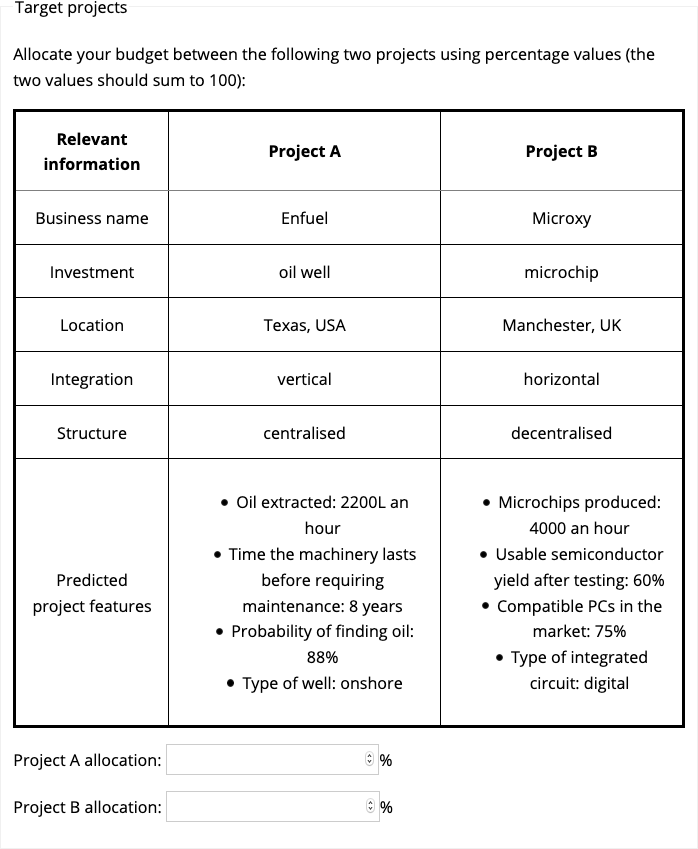
\includegraphics[width=1\linewidth]{thesis_files/figure-latex/project-allocation-anecdote-only-materials-anecdotes-1-1} \caption{Project display for the anecdote only condition in Experiment 1.}\label{fig:project-allocation-anecdote-only-materials-anecdotes-1}
\end{figure}



\begin{figure}
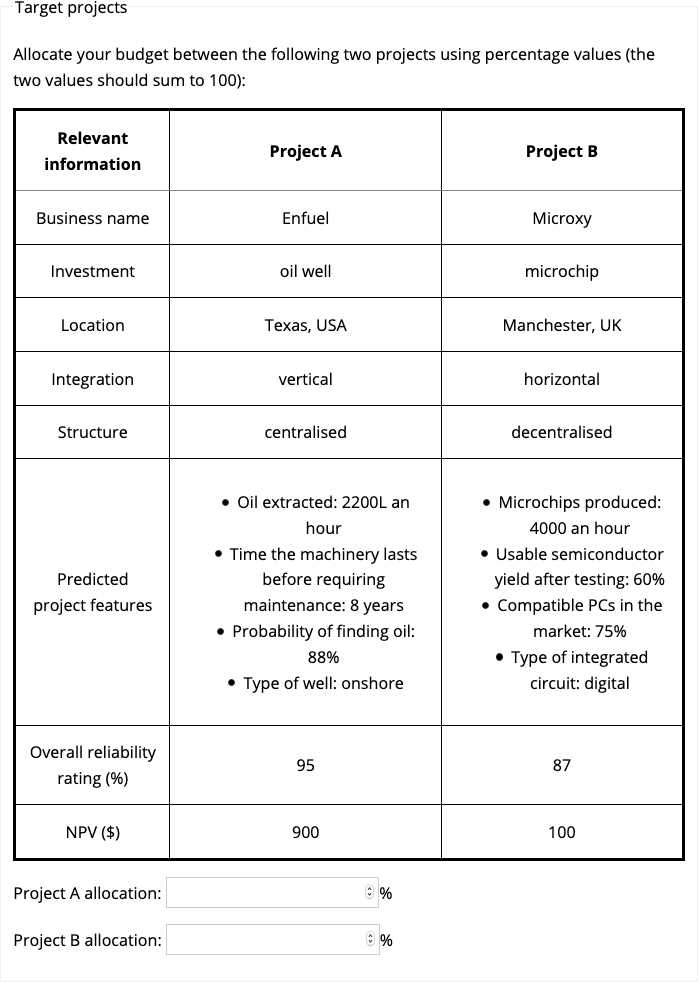
\includegraphics[width=1\linewidth]{thesis_files/figure-latex/project-allocation-statistics-materials-anecdotes-1-1} \caption{Project display for the statistics only, anecdote + statistics, and anecdote + enhanced statistics conditions in Experiment 1.}\label{fig:project-allocation-statistics-materials-anecdotes-1}
\end{figure}

\hypertarget{anecdote}{%
\paragraph{Anecdote}\label{anecdote}}

Participants that were presented with an anecdote (those in either the anecdote
only, anecdote + statistics , or anecdote + enhanced statistics conditions) saw
a description of a business project and an accompanying ``analysis.''
Figures~\ref{fig:anecdote-similarity-high-materials-anecdotes-1}
and~\ref{fig:anecdote-similarity-low-materials-anecdotes-1} show the anecdote
display for those in the high and low similarity conditions, respectively. The
project description had a similar layout to the target projects. That is, it
contained information about the business name, location, integration, and
organisational structure of the business, and detailed predicted features of the
project. Underneath this description was a paragraph of text that participants
were told was an analysis of why the project failed. Therefore, this text
references each of the features in the description in order to justify the
project failing.

Those in the high similarity condition saw a description of a project from a
business with the same type of investment. All categorical attributes were
identical to the relevant target project (Project A), and the numerical
attributes were all made to be lower than those in Project A. In the analysis,
the numerical attributes were explained to have failed because they were not as
high as certain cut-offs. Critically, these cut-offs were made to all be higher
than the relevant values in Project A. This was done to make sure that the
numerical attributes in the anecdote seem more relevant to those in Project A.
For instance, for Project A, oil extraction was 2200L an hour, for the anecdote
it was 2000L an hour, and the cutoff was 3000L an hour. As such, a failure of
the anecdote because of an insufficient oil extraction rated will seem more
relevant since they both share the state of being lower than the cut-off in the
analysis. Note, however, that there was uncertainty about the generalisability
of these cut-off values because the participants did not receive a explicit
indication about whether these values were meant to generalise to other cases.



\begin{figure}
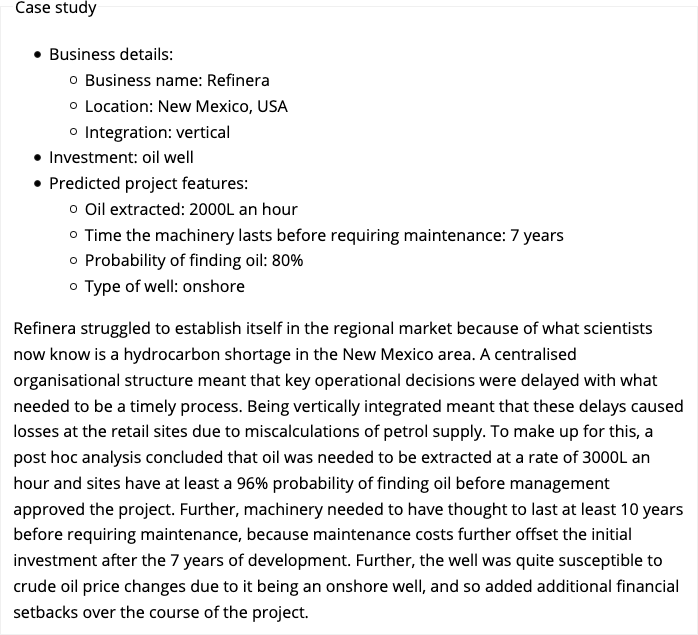
\includegraphics[width=1\linewidth]{thesis_files/figure-latex/anecdote-similarity-high-materials-anecdotes-1-1} \caption{Anecdote display for those in the high alignment condition in Experiment 1.}\label{fig:anecdote-similarity-high-materials-anecdotes-1}
\end{figure}



\begin{figure}
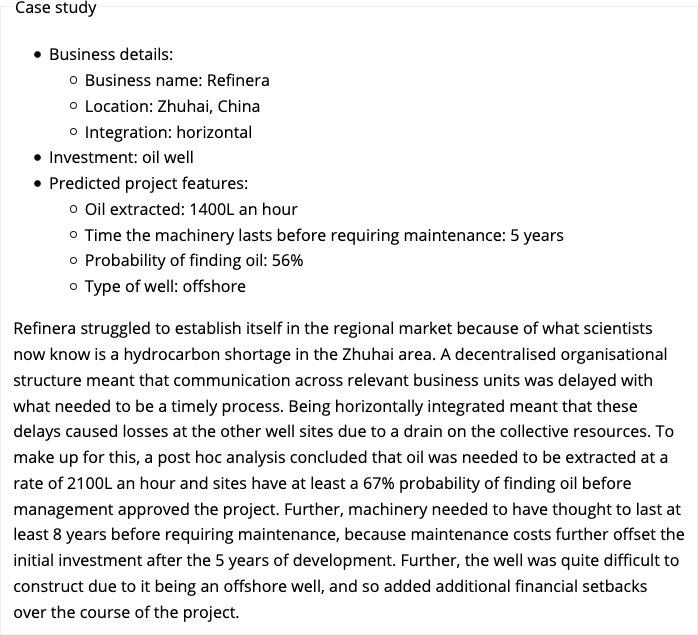
\includegraphics[width=1\linewidth]{thesis_files/figure-latex/anecdote-similarity-low-materials-anecdotes-1-1} \caption{Anecdote display for those in the low alignment condition in Experiment 1.}\label{fig:anecdote-similarity-low-materials-anecdotes-1}
\end{figure}

\hypertarget{follow-up-questions}{%
\paragraph{Follow-up questions}\label{follow-up-questions}}

Participants that saw the anecdote were subsequently presented with follow-up
questions. They were asked how similar they believe the anecdote was to the
target project, how relevant it was for their allocations, and how relevant it
would be for judgements about other projects of that type. See
Appendix~\ref{follow-up-materials-anecdotes-1} for a screenshot of the display.

\hypertarget{procedure-3}{%
\subsubsection{Procedure}\label{procedure-3}}

Following ethics and demographics web-pages, participants were introduced to the
study through the general instructions and the specific instructions relevant to
the condition. They then saw the allocation task, which included the anecdote
analysis and description (for those not in the statistics condition), and the target
projects description. Those that saw an anecdote were subsequently shown the
follow-up questions.

\hypertarget{results-anecdotes-1}{%
\subsection{Results}\label{results-anecdotes-1}}

\hypertarget{the-effect-of-similarity-on-anecdotal-bias}{%
\subsubsection{The effect of similarity on anecdotal bias}\label{the-effect-of-similarity-on-anecdotal-bias}}

Figure~\ref{fig:plot-anecdotes-1-allocation} shows the results for the
allocation data. I tested anecdotal bias by comparing the statistics only
condition with the high and low similarity anecdote + (not enhanced) statistics
conditions. The omnibus one-way ANOVA test of these three conditions was
significant, \(F(2, 120) = 4.40\), \(p = .014\), \(\hat{\eta}^2_p = .068\). Planned comparisons
revealed that participants allocated more to the target project when seeing only
statistics than when seeing the high similarity anecdote and statistics,
\(\Delta M = -12.78\), 95\% CI \([-21.90,~-3.66]\), \(t(120) = -2.77\), \(p = .006\); but not compared
to seeing the low similarity anecdote and statistics,
\(\Delta M = -2.17\), 95\% CI \([-11.29,~6.95]\), \(t(120) = -0.47\), \(p = .638\). Therefore, I
found evidence of anecdotal bias only in the high similarity condition.

\hypertarget{the-effect-of-enhanced-statistics}{%
\subsubsection{The effect of enhanced statistics}\label{the-effect-of-enhanced-statistics}}

To investigate the effect of enhanced statistics I compared the conditions in
which participants saw both an anecdote and statistics to the conditions in
which they saw the same, but with enhanced statistics. The two-way interaction
between similarity and the two anecdote + statistics conditions was not
significant, \(M = 4.12\), 95\% CI \([-8.56,~16.80]\), \(t(240) = 0.64\), \(p = .523\), as
was the main effect of anecdote + statistics condition (averaging over
similarity), \(\Delta M = -0.23\), 95\% CI \([-6.57,~6.11]\), \(t(240) = -0.07\), \(p = .943\). Therefore, I
did not find evidence that providing participants with instructions with how to
think statistically facilitated a focus on statistics.

\hypertarget{the-effect-of-statistics}{%
\subsubsection{The effect of statistics}\label{the-effect-of-statistics}}

A two-way ANOVA was conducted to investigate the interaction of similarity (low
and high) and anecdote conditions (anecdote only, statistics + anecdote,
excluding anecdote + enhanced statistics). This allowed me to identify the role
of statistics. The interaction between anecdote condition and similarity,
excluding the enhanced condition was significant,
\(M = -13.71\), 95\% CI \([-26.39,~-1.03]\), \(t(240) = -2.13\), \(p = .034\). Specifically, the
difference between allocations when only seeing an anecdote and seeing the
anecdote + statistics was greater when the anecdote was similar,
\(\Delta M = -21.56\), 95\% CI \([-32.30,~-10.83]\), \(t(240) = -4.74\), \(p < .001\); compared to when it
was dissimilar, \(\Delta M = -7.85\), 95\% CI \([-18.59,~2.88]\), \(t(240) = -1.73\), \(p = .198\).
Therefore, I found evidence of ``partial'' anecdotal bias in the high similarity
condition, since the anecdote + statistics condition was lower than the
statistics only condition, but higher than the anecdote only condition.



\begin{figure}
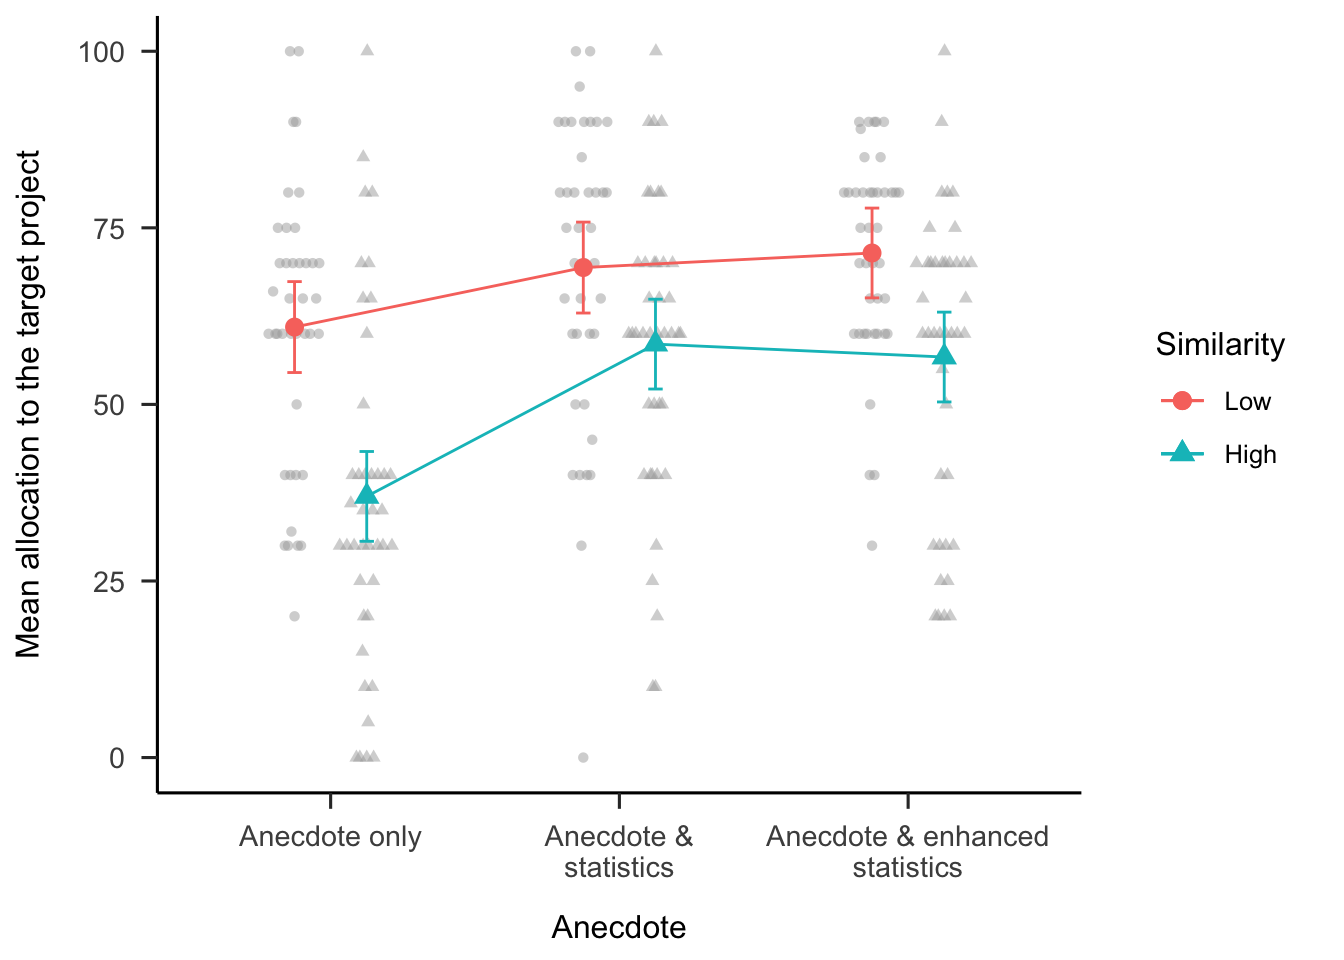
\includegraphics[width=1\linewidth]{thesis_files/figure-latex/plot-anecdotes-1-allocation-1} \caption{Mean allocation to Project A (the target project). Error bars represent 95\% confidence intervals.}\label{fig:plot-anecdotes-1-allocation}
\end{figure}

\hypertarget{relevance-ratings}{%
\subsubsection{Relevance ratings}\label{relevance-ratings}}

I conducted regression analyses to determine the relationship between
allocations and the follow-up relevance ratings. As seen in
Figure~\ref{fig:plot-anecdotes-1-lm-allocation-relevance-specific-alignment}
the specific relevance ratings interact with similarity condition,
\(b = -2.81\), 95\% CI \([-4.76, -0.86]\), \(t(242) = -2.83\), \(p = .005\). It appears
that specific relevance ratings are related to allocations, but only in the high
similarity condition. Further, there were no significant associations with the
general relevance ratings. This suggests that people are reasoning about the
connection between the anecdote and target, as opposed to simply reacting to the
failed project and associating that with the project industry.



\begin{figure}
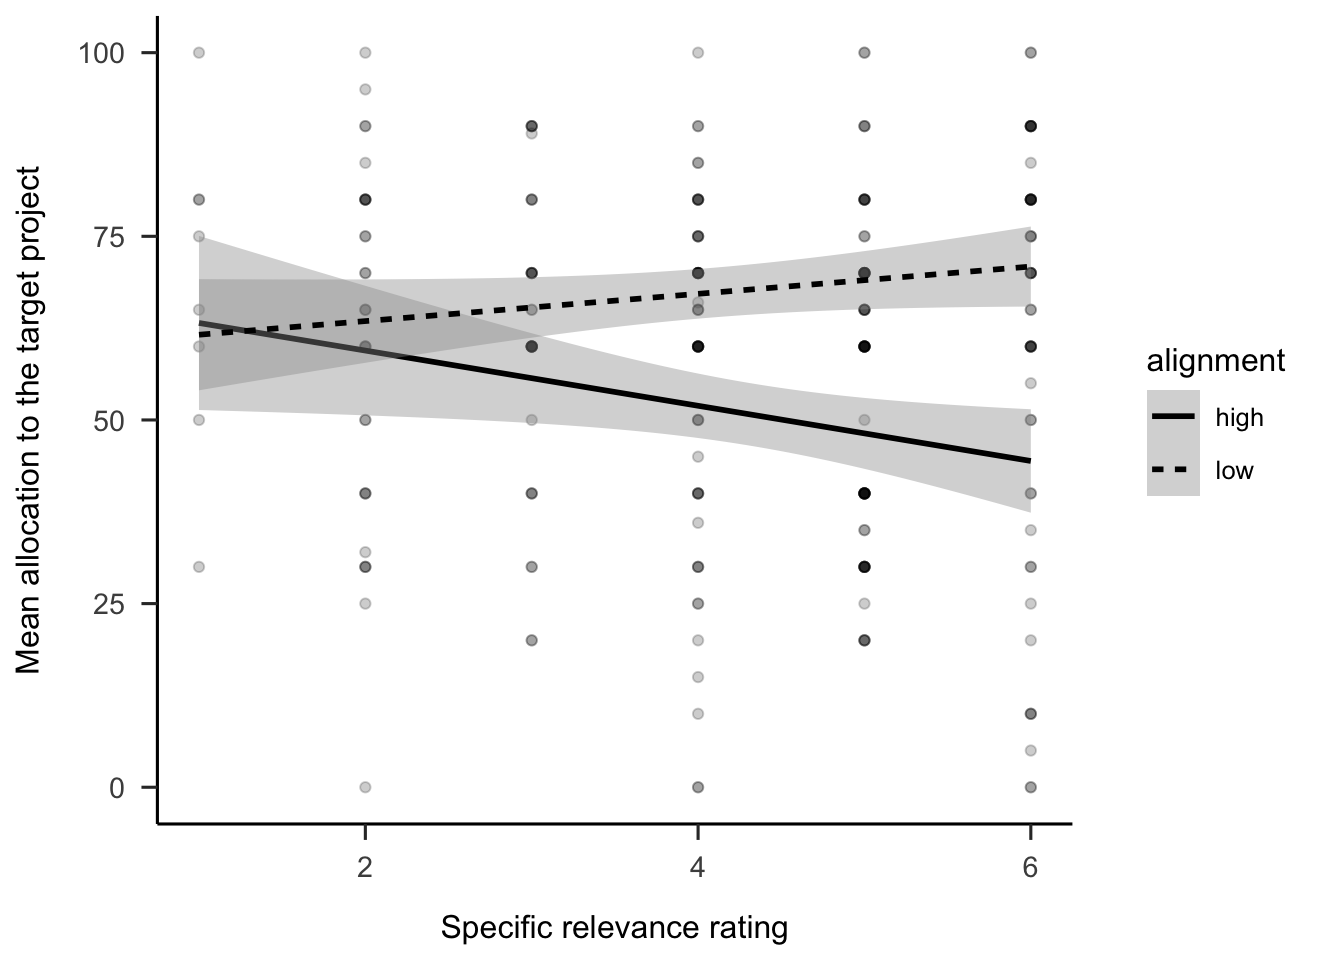
\includegraphics[width=1\linewidth]{thesis_files/figure-latex/plot-anecdotes-1-lm-allocation-relevance-specific-alignment-1} \caption{Mean allocations to the target project, by specific relevance rating and similarity condition.}\label{fig:plot-anecdotes-1-lm-allocation-relevance-specific-alignment}
\end{figure}

\hypertarget{discussion-4}{%
\subsection{Discussion}\label{discussion-4}}

I found support for Hypothesis~\ref{hyp:anecdote-similarity-anecdotes-1}, as
participants allocated less resources when seeing both the anecdote and
statistics, than when just seeing statistics, in the high similarity condition,
but not in the low similarity condition. This shows that while anecdotal bias
exists when the anecdote is similar, participants are not influenced when the
causal mechanisms do not match. Contrary to
Hypothesis~\ref{hyp:statistics-anecdotes-1}, I found that while participants
were influenced by the anecdote, they still made some use of the statistics.
This is different from \textcite{wainberg2013}, who found no difference between an
anecdote only and a anecdote + statistics condition, indicating a ``complete''
effect of anecdotal bias. Hypothesis~\ref{hyp:enhanced-statistics-anecdotes-1}
was also not supported, as the added enhanced statistical language used to
encourage participants to use the statistical information did not contribute to
reducing participants' reliance on anecdotes.

Experiment 1 was limited because it only considered an anecdote with a
\emph{negative} valence. That is, the case study was of a project that failed.
However, in real life these case studies are often ones with \emph{positive} valence.
That is, a story of a successful company. In fact, it may be the case that in
business, the anecdotes that are used are more likely to be positive, because of
survivorship bias. \textcite{jaramillo2019} found an anecdotal bias effect in negative
anecdotes, but not in positive anecdotes. This may be because the work was done
in medical decision-making and in this domain, a loss of health may be felt
stronger than an equivalent gain of health. Therefore, in Experiment 2 I added a
condition with a positive anecdote, in order to investigate whether anecdote
valence will impact the anecdotal bias effect.

Further, it was unclear if the effects found in Experiment 1 were related to
participants' perceptions of the type of sampling used in selecting the
anecdotes. The instructions in Experiment 1 do not explain how the anecdote that
is displayed to participants was chosen. Intentional or random sampling has been
shown to affect people's decision-making \autocite[e.g.,][]{hayes2019}. In the case of the
current experiments, the sampling assumption changes the extent to which it is
rational to use the anecdote or not. It may be considered rational to choose the
anecdote over the aggregated data if 1. the anecdote was not sampled randomly
from the pool of anecdotes, and 2. the anecdote is more similar to the target
project than any of the other anecdotes in the pool in relevant ways. That is,
if the anecdote was chosen because of its high relevance to the target project,
it would be irrational to ignore it. In Experiment 1 it was unclear whether
participants might have held these beliefs. In order to control for these
assumptions, in Experiment 2 I added text to the instructions that clarified
that the anecdote 1. was sampled randomly from the pool of anecdotes, and 2. is
not significantly more similar to the target project than any of the other
anecdotes in the pool.

\hypertarget{anecdotes-2}{%
\section{Experiment 2}\label{anecdotes-2}}

\protect\hyperlink{anecdotes-1}{Experiment 1} replicated the anecdotal bias effect. That is,
people use an anecdote more when presented with conflicting statistics than when
anecdote alone and less than when statistics alone. However, anecdote similarity
moderated this effect, such that anecdotal bias is stronger when the anecdote is
similar to the current task, than when it is dissimilar. Experiment 1 only used
a negative anecdote because previous research found anecdotal bias for negative,
but not for positive anecdotes \autocite{jaramillo2019}. However, \textcite{jaramillo2019}
considered medical decision-making, so this effect of anecdote valence may be
different in a business scenario. When considering medicine, it is likely that
negative anecdotes are more salient than positive ones. Positive health can
generally simply mean a lack of change of one's current state, whereas a
negative health outcome almost necessarily involves a change for the worse.
Further, Experiment 1 did not clarify certain assumptions about the way the
displayed anecdote was sampled from the pool of anecdotes.

Therefore, in Experiment 2 I added a within-subjects anecdote valence
manipulation and manipulated anecdote similarity within-subjects, in order to
increase the experiment's power. Further, I removed the anecdote + enhanced
statistics manipulation as Experiment 1 did not find evidence for its efficacy.
All participants saw the statistics only condition, as it did not contain an
anecdote, and therefore did not need to be manipulated between-subjects. Each
participant therefore saw five displays, with one statistics only condition, and
four displays for either the anecdote only condition, or the anecdote +
statistics condition. These four anecdote displays consisted of the similarity
(low and high) \(\times\) valence (negative and positive) conditions.

I expected to replicate the effects of Experiment 1, as well as seeing the
reverse effect in the positive valence condition. Also, I expected that
statistics will have an effect similar to Experiment 1, contrary to
Hypothesis~\ref{hyp:statistics-anecdotes-1}. Therefore, as well as again
testing Hypothesis~\ref{hyp:anecdote-similarity-anecdotes-1}, I tested the
following hypotheses (see Appendix~\ref{anecdotes-2-appendix} for a plot of a
simulation of all hypothesised effects):

\begin{hypothesis}[Overall effect]
\protect\hypertarget{hyp:three-way-anecdotes-2}{}{\label{hyp:three-way-anecdotes-2} \iffalse (Overall effect) \fi{} }Three-way interaction of similarity \(\times\) valence \(\times\) anecdote,
excluding statistics-only
\end{hypothesis}

\begin{hypothesis}[Anecdotal bias moderated by similarity for positive anecdotes]
\protect\hypertarget{hyp:anecdote-similarity-anecdotes-2}{}{\label{hyp:anecdote-similarity-anecdotes-2} \iffalse (Anecdotal bias moderated by similarity for positive anecdotes) \fi{} }When the anecdote is positive, allocations will be higher in the statistics-only
condition than in both the anecdote + statistics conditions (high and low
similarity). Within these two anecdote + statistics conditions, allocations will
be higher when the anecdote is similar than when it is dissimilar.
\end{hypothesis}

After not replicating the lack of a statistics effect as in \textcite{wainberg2013}, in
Experiment 2 I expected to replicate the finding in Experiment 1 that
participants do somewhat integrate statistics in their decisions. Therefore, I
tested the following hypotheses:

\begin{hypothesis}[Effect of statistics for negative anecdotes]
\protect\hypertarget{hyp:statistics-negative-anecdotes-2}{}{\label{hyp:statistics-negative-anecdotes-2} \iffalse (Effect of statistics for negative anecdotes) \fi{} }In the negative valence condition, allocations will be higher for the high
similarity anecdote + statistics condition than the high similarity
anecdote only condition.
\end{hypothesis}

\begin{hypothesis}[Effect of statistics for positive anecdotes]
\protect\hypertarget{hyp:statistics-positive-anecdotes-2}{}{\label{hyp:statistics-positive-anecdotes-2} \iffalse (Effect of statistics for positive anecdotes) \fi{} }In the positive valence condition, allocations will be higher for the high
similarity anecdote only condition than the high similarity statistics +
anecdote condition.
\end{hypothesis}

\hypertarget{method-5}{%
\subsection{Method}\label{method-5}}

\hypertarget{participants-6}{%
\subsubsection{Participants}\label{participants-6}}

Ninety-six (50 female) people were recruited from the online recruitment platform Prolific. Participants were compensated at a rate of £5 an hour. The average age was 41.69 (\emph{SD} = 11.29, \emph{min} = 27, \emph{max} = 74). Participants reported an average of 7.19 (\emph{SD} = 8.34, \emph{min} = 0, \emph{max} = 43) years of work in a business setting, and an average of 3.91 (\emph{SD} = 7.66, \emph{min} = 0, \emph{max} = 50) years of business education. The mean completion time was 15.01 (\emph{SD} = 8.73, \emph{min} = 2.57, \emph{max} = 58.71) minutes.~Table~\ref{tab:condition-allocation-anecdotes-2}
shows the between-subjects condition allocation. Similarity and valence were
manipulated within-subjects. Therefore, each participant was in one of two
between-subjects anecdote conditions, and saw five displays (statistics only,
and one for each similarity/valence combination).
Appendix~\ref{power-analysis-anecdotes-2} describes the power analysis
conducted to arrive at this sample size.

\begin{table}[tbp]

\begin{center}
\begin{threeparttable}

\caption{\label{tab:condition-allocation-anecdotes-2}Experiment 2 group allocation.}

\begin{tabular}{ll}
\toprule
Anecdote between & \multicolumn{1}{c}{N}\\
\midrule
Anecdote only & 48\\
Combined & 48\\
Total & 96\\
\bottomrule
\end{tabular}

\end{threeparttable}
\end{center}

\end{table}

\hypertarget{materials-4}{%
\subsubsection{Materials}\label{materials-4}}

\hypertarget{instructions-4}{%
\paragraph{Instructions}\label{instructions-4}}

Participants were shown similar instructions to \protect\hyperlink{instructions-materials-anecdotes-1}{Experiment
1}. I also included a test of basic
instructions understanding that also functioned as an attention check. As in
Experiment 1, participants also saw instructions that were specific to their
condition. These were shown on the same page as the rest of the project display,
above the case study and target projects. One important difference from
Experiment 1 was that I clarified in the instructions text both that the
anecdote was sampled randomly and that the anecdotes in the pool were all
equally similar to the target project.
Appendix~\ref{instructions-materials-anecdotes-2-appendix} shows screenshots of
these web-pages.

\hypertarget{allocation-anecdotes-2}{%
\paragraph{Allocation task}\label{allocation-anecdotes-2}}

As in Experiment 1, the allocation task included a description and analysis of
an anecdote (except for those in the anecdote only condition) and a project
display with a table describing the two target projects.
Figures~\ref{fig:project-allocation-anecdote-valence-negative-similarity-low-materials-anecdotes-2}
and~\ref{fig:project-allocation-target-valence-negative-similarity-low-materials-anecdotes-2}
show the anecdote and target projects for the negative valence low similarity
condition, respectively.
Figures~\ref{fig:project-allocation-anecdote-valence-positive-similarity-high-materials-anecdotes-2}
and~\ref{fig:project-allocation-target-valence-positive-similarity-high-materials-anecdotes-2}
show the anecdote and target projects for the positive valence high similarity
conditions, respectively. In the statistics only condition, participants only
saw the target projects display. Appendix~\ref{allocation-anecdotes-2-appendix}
details the counterbalancing and randomisation that I used.



\begin{figure}

\includegraphics[width=1\linewidth]{thesis_files/figure-latex/project-allocation-anecdote-valence-negative-similarity-low-materials-anecdotes-2-1} \caption{An example of the anecdote display in the negative valence, low similarity condition of Experiment 2.}\label{fig:project-allocation-anecdote-valence-negative-similarity-low-materials-anecdotes-2}
\end{figure}



\begin{figure}
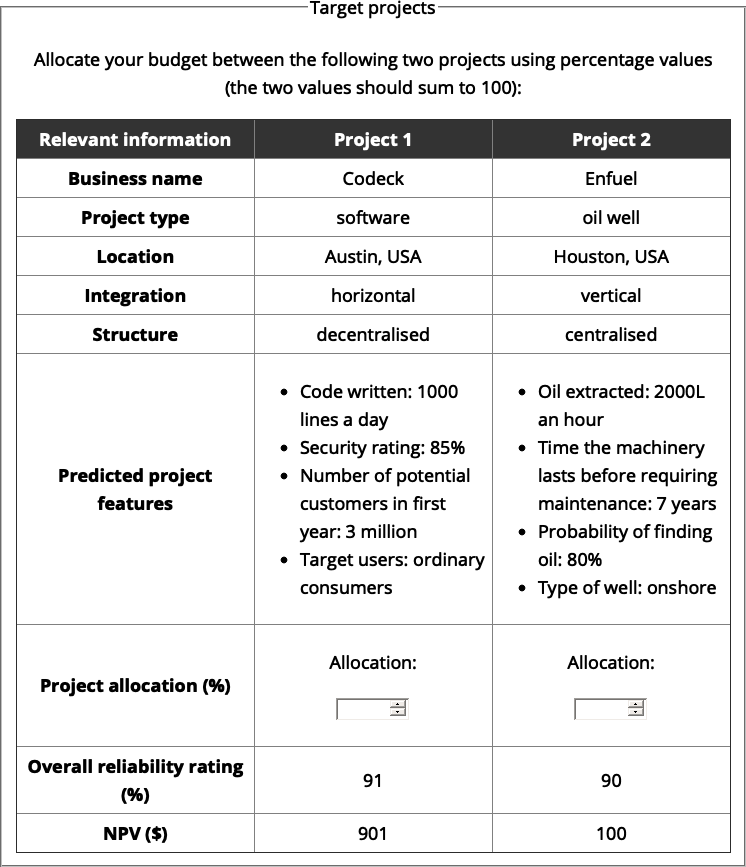
\includegraphics[width=1\linewidth]{thesis_files/figure-latex/project-allocation-target-valence-negative-similarity-low-materials-anecdotes-2-1} \caption{An example of the target projects in the negative valence, low similarity condition of Experiment 2.}\label{fig:project-allocation-target-valence-negative-similarity-low-materials-anecdotes-2}
\end{figure}



\begin{figure}

\includegraphics[width=1\linewidth]{thesis_files/figure-latex/project-allocation-anecdote-valence-positive-similarity-high-materials-anecdotes-2-1} \caption{An example of an anecdote display in the positive valence, high similarity condition of Experiment 2.}\label{fig:project-allocation-anecdote-valence-positive-similarity-high-materials-anecdotes-2}
\end{figure}



\begin{figure}
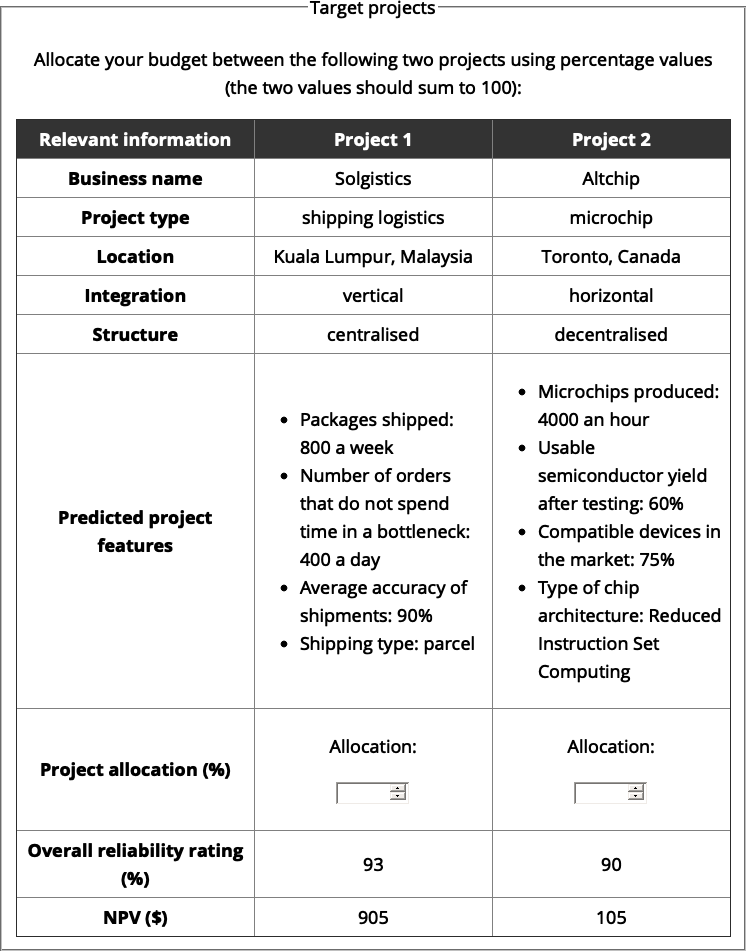
\includegraphics[width=1\linewidth]{thesis_files/figure-latex/project-allocation-target-valence-positive-similarity-high-materials-anecdotes-2-1} \caption{An example of the target projects in the positive valence, high similarity condition of Experiment 2.}\label{fig:project-allocation-target-valence-positive-similarity-high-materials-anecdotes-2}
\end{figure}

\hypertarget{interstitial-3}{%
\paragraph{Interstitial}\label{interstitial-3}}

Before each display, participants saw an ``interstitial'' page, whose role was 1.
to introduce the next display, and 2. to provide an attention check (not
required to answer, so can be skipped if the interstitial text isn't read). See
Appendix~\ref{interstitial-materials-anecdotes-2}.

\hypertarget{follow-up-questions-1}{%
\paragraph{Follow-up questions}\label{follow-up-questions-1}}

Participants were shown similar follow-up questions as in Experiment 1, except
that here the rating scales were 1-7, instead of 1-6. See
Appendix~\ref{follow-up-materials-anecdotes-2} for an example of a follow-up
display.

\hypertarget{procedure-4}{%
\subsubsection{Procedure}\label{procedure-4}}

Following ethics and demographics web-pages, participants were introduced to the
study through the general instructions. They then saw five sets of two web-pages
(in randomised order). Each ``set'' contained two web-pages: the allocation task
and a follow-up questions page (except for the anecdotes only condition, in
which participants did not see the follow-up questions page). Each allocation
task page contained specific instructions relevant to the condition, followed by
the anecdote analysis and description, and the target projects description. The
only exception was the statistics only display, for which there was no anecdote
description or analysis.

\hypertarget{results-3}{%
\subsection{Results}\label{results-3}}

I analysed the allocation data that was relevant to the Experiment 2 hypotheses.
See Appendix~\ref{results-anecdotes-2-appendix} for manipulation check
analyses, and analyses of the follow-up rating data.

\hypertarget{overall-effect-of-manipulations}{%
\subsubsection{Overall effect of manipulations}\label{overall-effect-of-manipulations}}

As seen in Figures~\ref{fig:plot-anecdotes-2-allocation-negative}
and~\ref{fig:plot-anecdotes-2-allocation-positive}, the similarity \(\times\)
valence \(\times\) anecdote interaction (excluding the statistics-only condition)
was not significant,
\(F(1, 94) = 3.42\), \(p = .067\), \(\hat{\eta}^2_p = .035\).
However, the similarity \(\times\) valence interaction was significant,
\(F(1, 94) = 76.41\), \(p < .001\), \(\hat{\eta}^2_p = .448\) as was the anecdote \(\times\) valence
interaction, \(F(1, 94) = 10.11\), \(p = .002\), \(\hat{\eta}^2_p = .097\).

\hypertarget{anecdotal-bias-moderated-by-similarity}{%
\subsubsection{Anecdotal bias moderated by similarity}\label{anecdotal-bias-moderated-by-similarity}}

To investigate whether anecdotal bias was moderated by similarity, I compared
allocations between the anecdote + statistics high and low similarity conditions and the
statistics-only condition. I found that in the negative valence condition,
participants allocated more in the statistics-only condition than in the
anecdote + statistics high similarity condition,
\(\Delta M = -19.25\), 95\% CI \([-29.66,~-8.84]\), \(t(141) = -3.65\), \(p < .001\).
Participants in the anecdote + statistics low similarity allocated more than when they saw
the anecdote + statistics high similarity display,
\(\Delta M = -18.17\), 95\% CI \([-28.58,~-7.75]\), \(t(141) = -3.45\), \(p = .001\).
However, the difference between responses to the statistics-only projects and
the anecdote + statistics low similarity projects was not significant,
\(\Delta M = -1.08\), 95\% CI \([-11.50,~9.33]\), \(t(141) = -0.21\), \(p = .837\)
This provides evidence for the moderation of anecdotal bias by similarity for
negative anecdotes.

In the positive valence condition, allocations were higher in the statistics-only
condition than in the anecdote + statistics low similarity condition,
\(\Delta M = -31.73\), 95\% CI \([-41.86,~-21.60]\), \(t(141) = -6.19\), \(p < .001\).
Allocations were also higher in the anecdote + statistics high similarity condition than in
the anecdote + statistics low similarity condition,
\(\Delta M = 14.10\), 95\% CI \([3.97,~24.23]\), \(t(141) = 2.75\), \(p = .007\).
Further, allocations were higher in the statistics-only condition than in the
anecdote + statistics high similarity condition,
\(\Delta M = -17.62\), 95\% CI \([-27.75,~-7.50]\), \(t(141) = -3.44\), \(p = .001\).
This provides evidence for the moderation of anecdotal bias by similarity for
positive anecdotes.

\hypertarget{effect-of-statistics}{%
\subsubsection{Effect of statistics}\label{effect-of-statistics}}

As in Experiment 1, I investigated the extent to which the statistical
information influenced participants' allocations. When in the negative valence
condition, participants allocated more to the high similarity anecdote +
statistics project than those in the high similarity anecdote-only condition,
\(\Delta M = -12.67\), 95\% CI \([-23.53,~-1.81]\), \(t(336.36) = -2.29\), \(p = .022\).
When in the positive valence condition, they allocated more to the high similarity
anecdote-only condition than those in the high similarity anecdote + statistics condition,
\(\Delta M = 16.71\), 95\% CI \([5.85,~27.57]\), \(t(336.36) = 3.03\), \(p = .003\). This provides
evidence for the influence of statistics on participants' allocations for both
negative and positive anecdotes.



\begin{figure}
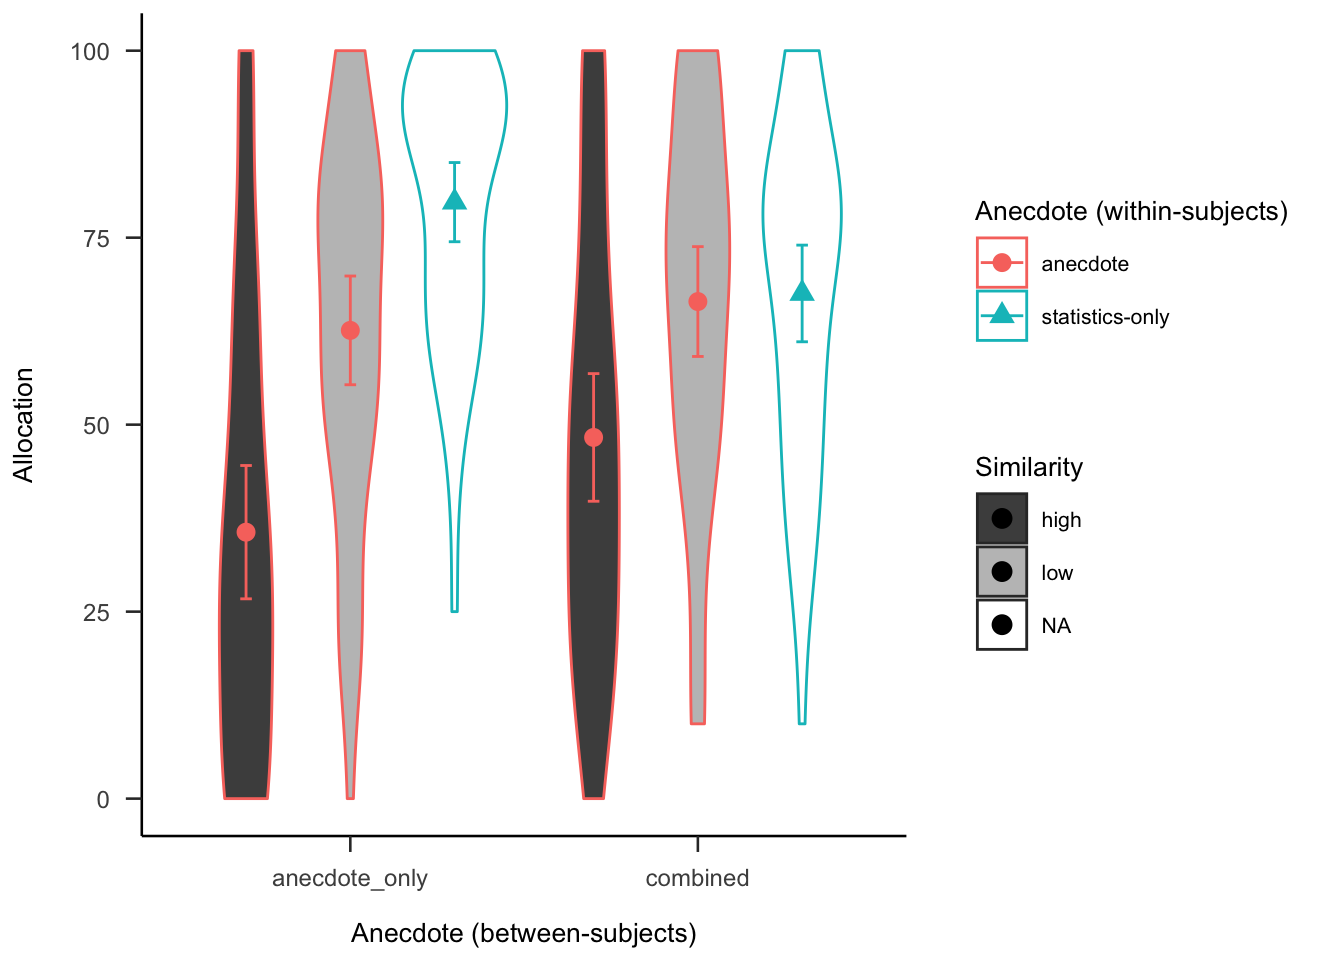
\includegraphics[width=1\linewidth]{thesis_files/figure-latex/plot-anecdotes-2-allocation-negative-1} \caption{Mean allocation in Experiment 2 for the positive valence condition.}\label{fig:plot-anecdotes-2-allocation-negative}
\end{figure}



\begin{figure}
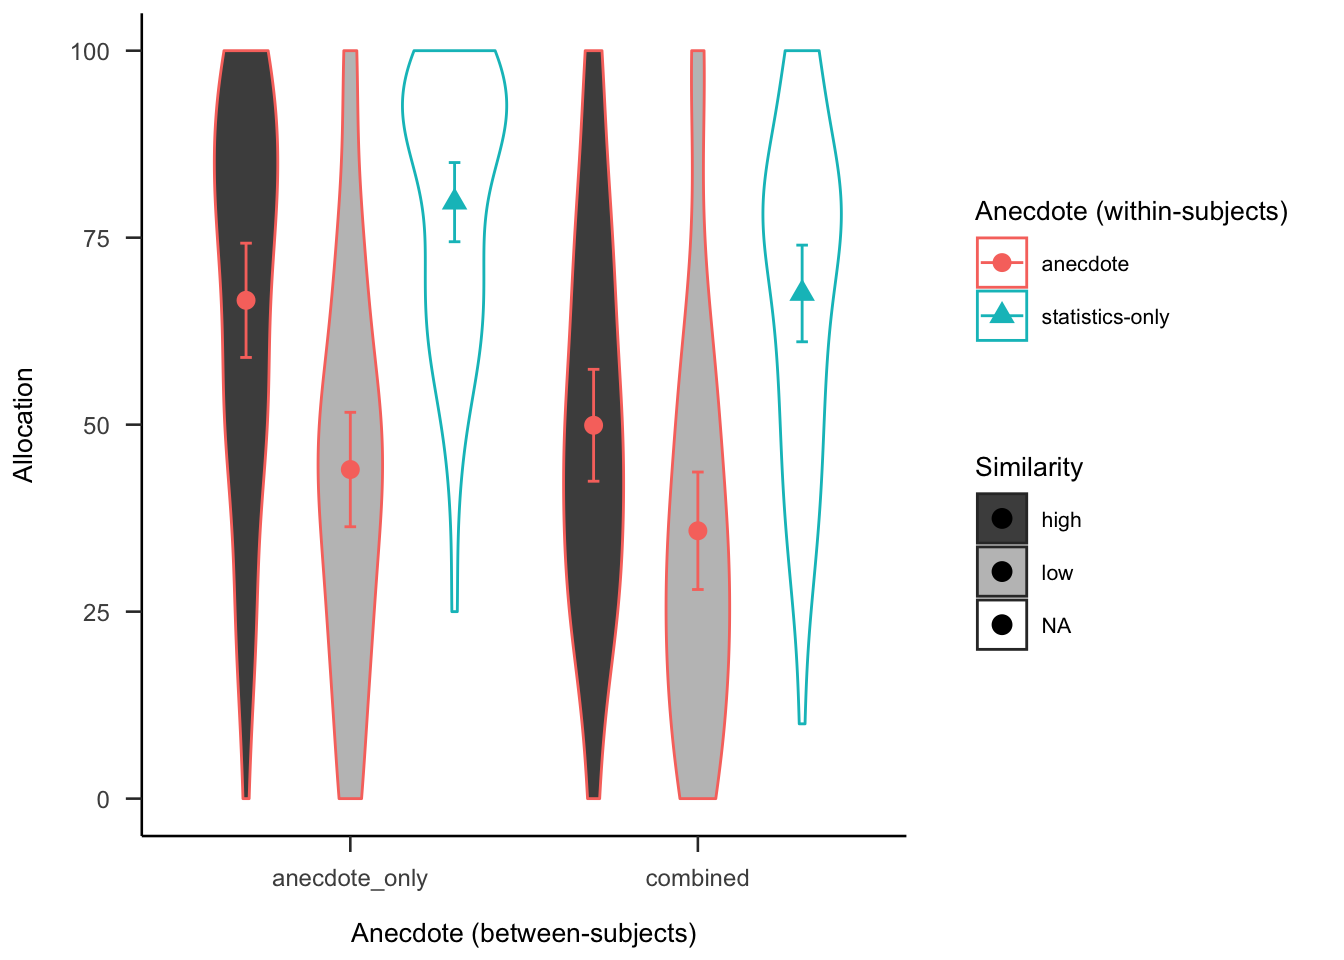
\includegraphics[width=1\linewidth]{thesis_files/figure-latex/plot-anecdotes-2-allocation-positive-1} \caption{Mean allocation in Experiment 2 for the positive valence condition.}\label{fig:plot-anecdotes-2-allocation-positive}
\end{figure}

\hypertarget{discussion-5}{%
\subsection{Discussion}\label{discussion-5}}

I found support for Hypothesis~\ref{hyp:anecdote-similarity-anecdotes-1} and
Hypothesis~\ref{hyp:anecdote-similarity-anecdotes-2}, as participants showed a
stronger anecdotal bias effect when the anecdote was more similar to the target
project, both for positive and negative anecdotes. Further, as per
Hypothesis~\ref{hyp:statistics-negative-anecdotes-2} and
Hypothesis~\ref{hyp:statistics-positive-anecdotes-2}, I found that participants
seemed to incorporate the statistical information into their judgements, in both
negative and positive anecdotes.

Experiment 2 therefore found that, unlike in the medical domain, the effect of
anecdotes in financial decision-making does not seem to depend on anecdote
valence. Further, as in Experiment 1, and unlike \textcite{wainberg2013}, the anecdotal
bias effect does not seem to be complete, with statistics still playing some
role in participants' decisions despite the effect of the anecdote.

\hypertarget{general-discussion-2}{%
\section{General discussion}\label{general-discussion-2}}

Most of the hypotheses were supported. I found that people's decisions are
influenced by anecdotes even when aggregated data is available in a
resource-allocation context. I also made three novel findings: 1. I found that
the anecdotal bias effect is only seen when participants consider the anecdote
as sufficiently relevant to the target at hand, 2. participants still seem to
integrate statistics in their decisions, and 3. these effects are seen in both
negative and positive anecdotes.

The first novel finding from these experiments was that participants appeared to
moderate their use of anecdotal evidence. Specifically, when the anecdote
appeared to be causally relevant, participants used it in their decisions.
However, when it appeared irrelevant, participants relied on statistics almost
entirely. The findings in the high similarity condition are largely congruent
with findings from other work investigating anecdotal bias in business
decision-making. As in \textcite{wainberg2013} and \textcite{wainberg2018}, I found that people
allocate less resources to a project that is successful according to statistical
evidence, but is displayed alongside a contradictory similar anecdote, than to a
project with just the statistics.

It seems that participants made the distinction between the low and high
similarity conditions based on underlying structure of the anecdote. The low
similarity condition always consisted of the same project type, for each domain,
as in the high similarity condition. For instance, in one variation, both the
high and low similarity anecdotes were of oil well projects. This means that
participants were sensitive to the specific information presented to them in the
anecdote description and ``analysis,'' and did not simply use the project type for
their inferences. Further, participants' answers to the follow up questions
indicated that, while they considered that the anecdote was relevant in when
considering the target project, they did not consider it as relevant to other
such projects. In other words, participants did not appear to carelessly use
anecdotal evidence in their decisions, but instead appeared to carefully
consider the anecdote based on its particular causal structure.

The second novel finding from these experiments was that participants that saw
both statistics and anecdotal evidence did not completely disregard the
statistical measures. \textcite{wainberg2013} found a ``complete'' effect of anecdotal bias,
because in their study, these two conditions were equivalent. This meant that
the statistics they provided had a negligible effect on participants' decisions.
These experiments, on the other hand, showed a ``partial'' anecdotal bias effect,
with allocations being different between when participants saw only an anecdote
and when they also saw the statistics. It seems as if participants integrated
the anecdote with the statistical information. As mentioned above, this suggests
that people's evaluation of evidence might be more sensitive than previously
thought.

This discrepancy might be a result of the sampled population. Since \textcite{freling2020}
found a stronger effect of anecdote when decisions were more personally
relevant, the manager sample in \textcite{wainberg2013} may have simply been more
personally invested in the task than the laypeople in the experiments in this
chapter. Similarly, \textcite{yang2015} found that anxiety increases anecdotal bias in
risky choice. It might also be due to the anecdote + statistics condition not
being equivalent between \textcite{wainberg2013} and the present work. Specifically, the
statistics shown in the anecdote + statistics condition in \textcite{wainberg2013} were
not the same ones that were shown in the same study's statistics only condition,
unlike in both the present experiments and \textcite{wainberg2018}. Instead, it was the
anecdote + enhanced statistics condition that contained the same statistics as
in the statistics only condition. This suggests that people integrate statistics
when they are sufficiently clear and no further interpretation is required.

The third novel finding from these experiments was that anecdotal bias was seen
in both negative and positive anecdotes. Most studies in the literature
considered anecdotes that involve an example with negative consequences (a
\emph{negative} anecdote). For instance, a medication that leads to an adverse
reaction in a patient. However, there is not much work in the literature that
involves an anecdote with positive consequences (a \emph{positive} anecdote).
\textcite{jaramillo2019} found an asymmetry in the effect of the anecdote, such that the
effect was stronger when a person in a description did not get better after a
medication (negative), compared to when they did get better (positive). In the
present experiments I found a more symmetrical effect, such that both the
effects of the moderated anecdotal bias and the influence of statistics were
found in both valence conditions. The difference between this and the finding
from \textcite{jaramillo2019} might be due to the domain of the task in that people are
more focused on negative outcomes in the medical domain.

\hypertarget{theoretical-implications-1}{%
\subsection{Theoretical implications}\label{theoretical-implications-1}}

The current work adds to the current understanding of the way people use
different forms of evidence in their decision-making. Previous work mostly
investigated the relative influence of statistics and anecdotes by comparing
anecdote and statistics conditions. The current work shows that comparing a
joint anecdote + statistics condition to both an anecdote only and statistics
only condition allows for a more specific representation of participants'
anecdotal bias. The influence of anecdote can be seen in the comparison between
statistics only and the anecdote + statistics condition, but the effect of
statistics can be seen in the comparison between the combined condition and the
anecdote only condition. These two effects allow to determine the independent
influence of anecdote and statistics, respectively. Further use of such a design
in future research might help to further understand the conditions under which
these types of evidence are used.

It seems that in some of the anecdotal bias literature there is an assumption
that using anecdotal evidence over statistical evidence is necessarily
irrational. This likely arises from examples from the medical domain in which
such decisions are indeed irrational (e.g., believing that vaccines cause
certain disorders despite the available evidence). In such cases, people
over-rely on anecdotes and should be relying more on aggregated data. However, a
case could be made for a rational use of anecdote based on the similarity of the
anecdote to the target. For instance, there are times in which an anecdote is so
similar to the target situation (e.g., the identical twin example in the
\protect\hyperlink{effect-of-similarity-anecdotes}{Introduction}) that it would be unwise not to
consider the anecdote. That is, the use of anecdote should depend on both 1. the
strength of the underlying causal structure between it and the target problem,
and 2. the distribution of similarity across cases in the sample on which the
statistics are based. People should use an anecdote when casual structure is
significantly more relevant than other cases in available data. It is also
important to note that there could also be misleading similarity. For instance,
if someone is highly similar, but not along some key hidden dimension that is
the real causal thing to care about, then using the anecdote may be the wrong
thing to do. What seems to be important is a sensitivity to relational, rather
than surface level similarity. Future research should further investigate how
varying the assumptions that people have about sampling from a data set of
anecdotes influences their anecdotal bias. Such assumptions can include the size
of the sample and the shape of the distribution.

\hypertarget{practical-implications-1}{%
\subsection{Practical implications}\label{practical-implications-1}}

The current work can contribute to managerial decision making by suggesting
insights into how managers make decisions about business case studies and
statistical information about certain industries. Managers of large companies
are often in a difficult position; they have incomplete information and an
uncertain environment. Despite this, different biases and responses to those
biases can be anticipated for different levels of uncertainty. For instance, a
manager may be in a position in which they are presented with both a convincing
case study that suggests a certain course of action, and also be in the
possession of aggregated data. The manager needs to be able to weigh the
evidence accordingly. The work in this chapter suggests that there are three
elements to consider: 1. the quality of the aggregated data (determined by
factors such as the sample size), 2. the relative similarity of the cases in the
data pool to the situation at hand, and 3. the similarity of the anecdote to the
situation at hand. For instance, if the anecdote is uniquely similar to the
target situation, and it is significantly more similar than the rest of the
cases in the data set, then it should have more weight than an anecdote that
comes from a pool of cases that are all just as similar to the target.

In a situation in which aggregated data is not available, however, managers
should rely more on anecdotes that are more similar in causal structure. That
is, they should be wary of merely using the surface similarity to make
inferences, and instead consider the underlying relational structures. The
present data suggest that laypeople can do this to an extent, with participants
not being completely swayed by the mere similarity of the type of business
project. However, future research should investigate this further to better
understand the boundaries of people's analogical reasoning in such situations.

\newpage

\printbibliography[segment=\therefsegment,heading=subbibintoc]



\begin{savequote}
work\ldots primarily concerned with the psychological processes that
govern judgment and inference\ldots portrayed people as fallible, not
irrational.
\qauthor{---Amos Tversky}\end{savequote}

\hypertarget{discussion}{%
\chapter{Discussion}\label{discussion}}

\minitoc

This thesis investigated the psychology of resource allocation decisions. The
influence of psychological factors on such decisions has not been sufficiently
considered in the literature despite its importance to the performance of
hierarchical organisations. This discrepancy is likely due to a greater focus of
the role of organisational influences on firm performance in the management
literature. The thesis did not investigate expertise effects, but instead
focused largely on participants without management experience. This allowed a
study of the specific cognitive processes without the potential confound of
experience. Each of the empirical chapters investigated distinct but related
processes that are relevant to the resource allocation process. By doing this I
was able to investigate whether people are able to account for the benefits of
aggregation when considering multiple projects (Chapter~\ref{aggregation}), the
influence of project feature alignability and metric variance when comparing
projects directly (Chapter~\ref{alignment}), and the influence of project
anecdote similarity when the anecdote conflicts with statistical evidence
(Chapter~\ref{anecdotes}). I will first summarise the results of the empirical
chapters and then discuss their theoretical and practical implications.

\hypertarget{summary-of-results}{%
\section{Summary of results}\label{summary-of-results}}

Chapter~\ref{aggregation} investigated the choice of risky business projects
that are displayed sequentially and without feedback. This design modelled the
real-life situation that managers are faced with in hierarchical organisations:
an evaluation of a set of separate business project proposals over time with no
immediate indication of the performance of those projects. Aggregating a
portfolio of such projects is likely to show a lower chance of potential loss
overall than might be originally assumed. The results from this chapter showed
that people not only did not do this spontaneously, but also were not
facilitated by manipulations that encouraged grouping choices together as a
portfolio. People only seemed to recognise the benefits of aggregation when they
were presented with an outcome probability distribution of the aggregated set of
projects. There was no strong evidence that more subtle manipulations aimed at
encouraging aggregation worked. Specifically, presenting projects together,
specifying the total number of projects, and presenting projects that were all
from the same industry did not encourage aggregation.

Chapter~\ref{alignment} investigated resource allocation when projects were
evaluated jointly and capital was allocated as a proportion of the budget,
rather than a binary choice. I manipulated whether all the project attributes
were alignable, or only the abstract financial metric (NPV) was alignable. I
also manipulated whether NPV was to be considered a reliable metric or not, and
whether this information was expressed as explicit verbal instruction or as
numerical ranges. The results showed that when reliability information was
presented verbally, participants used it appropriately when all project
attributes were completely alignable. That is, they used it when it was reliable
and used the intrinsic project features when it was unreliable. When only NPV
was alignable, participants relied on it regardless of the reliability
information. However, when reliability information was presented numerically,
there was no moderation of allocation based on the ranges---participants used
NPV even when they had an opportunity to use the intrinsic features of the
project. Overall, however, participants tended to rely on NPV more in the low
alignment condition than in the high alignment condition.

Chapter~\ref{anecdotes} investigated the effect of anecdote similarity on
allocations when anecdote conflicted with statistical data. Participants were
asked to allocate a hypothetical budget between two projects. One of the
projects was clearly superior in terms of the provided statistical measures, but
some of the participants also saw a description of a project with a conflicting
outcome. This anecdotal project was always in the same industry as one of the
target projects. However, the anecdote description either contained substantive
connections to the target or not. I also manipulated whether the anecdote
conflicted with the statistical measures because it was successful (positive
anecdote) or unsuccessful (negative anecdote). The results showed that
participants' decisions were influenced by anecdotes only when they believed
that they were actually relevant to the target project. Further, they still
incorporated the statistical measures into their decision. I found this for both
positive and negative anecdotes. However, participants were given information
about the way that the anecdotes were sampled that suggested that the
statistical information should have been used in all cases. Participants did not
use this information in their decision and still showed an anecdotal bias
effect. Therefore, people seem to appropriately moderate their use of anecdotes
based on the anecdotes' relevance, but do not understand the implications of
more complex statistical principles.

Together, these results show the bounds of people's decision-making capability
in resource allocation. The participants in these experiments in general behaved
rationally but struggled to incorporate more advanced statistical principles
into their decisions. Further, when confronted with multi-attribute choice,
participants tended to allocate resources using a trade-off strategy. This was
seen in the conflict between intrinsic project attributes and NPV in
Chapter~\ref{alignment} and the conflict between the anecdotal and statistical
evidence in Chapter~\ref{anecdotes}. Participants were able to moderate their
allocations when the moderating factors were sufficiently clear (as in the
verbal reliability condition in Chapter~\ref{alignment}). However, participants
struggled to do this when the moderating factor involved an understanding of a
more advanced statistical principle. Each empirical chapter included such a
principle: risk aggregation in Chapter~\ref{aggregation}, metric variance in
Chapter~\ref{alignment}, and sample distribution in Chapter~\ref{alignment}.
However, a formal understanding of such principles does not seem to be necessary
if they are expressed explicitly (as in the aggregated distribution in
Chapter~\ref{aggregation}).

\hypertarget{theoretical-implications-2}{%
\section{Theoretical implications}\label{theoretical-implications-2}}

The main theoretical contribution of this thesis is the addition of evidence
that further specifies the conditions under which people make rational decisions
in resource allocation scenarios. People made good decisions most of the time,
but sometimes do not take into account important moderating factors in their
decisions. Amos Tversky explained in his response to \textcite[p.~355]{cohen1981} that
the work on heuristics and biases ``portrayed people as fallible, not
irrational.'' That is, people are not constantly making mistakes, but often
behave rationally, largely due to adaptive heuristics. However, sometimes
shortcuts that are usually helpful can fail. Studying such biases is similar to
the way that optical illusions help understand the visual system. In both cases,
these are systems that most of the time function properly, but sometimes reveal
deficits.

Similarly, \textcite{simon1955} identified human rationality as \emph{bounded}, meaning that
people's cognitive processes are limited. The main aim of the thesis was to
contribute evidence for the ways that resource allocation decisions are bounded.
To this end, in each experiment, participants were given resource allocation
scenarios alongside both cues that describe their options and cues that frame
the options in different ways. Identifying which cues were used by participants
in their decisions, which cues were ignored, and which cues were integrated
allowed to specify the bounds of people's cognitive capacity in these decisions.
The experiments showed that people struggle to use certain statistical
principles in their decisions, but that they are also capable of making nuanced
trade-offs and can be assisted by decision aides.

In Chapter~\ref{aggregation} I presented participants with a resource
allocation situation in which an understanding of risk aggregation would have
led to beneficial outcomes. Investing in all the hypothetical projects would
have led to a much higher chance of gaining money than losing any. Each choice
bracketing manipulation provided a hint of the possibility of combining the
choices in this way. However, participants did not need to compute the
aggregated value of the prospects themselves. An intuitive understanding of
aggregation involved considering that of all the gambles some will pay-off and
make up for those that lost. However, this was not seen, with only weak evidence
that people were influenced by the more subtle choice bracketing manipulations.
Instead, people only seemed to respond to the principle of aggregation when it
was explicitly showcased. Showing people a distribution of the outcome
probabilities explicitly visualised the extent to which an aggregation of the
risks can lead to an incredibly low chance of loss.

In Chapter~\ref{alignment} the NPVs that participants saw were critical to the
allocation task. In the low alignment condition, NPV was the only alignable
attribute in the comparison. In the high alignment condition, however, NPV was
in competition with the intrinsic project feature values. An understanding of
numerical variance would have allowed participants to moderate their allocations
according to the implied reliability of the comparison metric. In the low
alignment condition, NPV was the only easy way to compare across projects, so it
was a more useful cue than the rest of the non-alignable values. However, in the
high alignment condition, the extent of numerical variance associated with each
NPV could have been used to determine NPV reliability. There were two ways to do
this: 1. noticing that in the low numerical reliability condition the ranges
were all overlapping, and 2. noticing the difference in the width of the ranges
between the two within-subjects reliability amount conditions. By doing this,
participants would have then been able to know to (in the high alignment
condition) use NPV when ranges were narrow and use the intrinsic values more or
exclusively when ranges were wider and overlapping. Participants were able to do
this sort of moderated allocation when reliability was expressed explicitly as
words, but not when it was expressed numerically.

In Chapter~\ref{anecdotes} participants did not make use of important
information about the sample distribution. As in Chapter~\ref{alignment},
participants were confronted with a conflict of cues: statistical information
vs.~a potentially relevant anecdote. Regardless of the similarity manipulation,
a consideration of the sample from which the anecdote was sampled should have
informed how the anecdote was used. Imagine a distribution that represents the
similarity of all the individual projects in the sample. That is, the x-axis
represents the similarity to the target project and the y-axis is the frequency
of projects that represent each level of similarity. Even if the sampled
anecdote appears very relevant to the target project, if the underlying
distribution of the sample is highly negatively skewed, such that most projects
in the sample are equivalently similar to the target, then the sampled anecdote
is not necessarily more informative than the aggregated measure. On the other
hand, if the underlying distribution was negatively skewed, normally
distributed, or even uniform, then the fact that the sampled anecdote appears
highly relevant to the target project may actually mean that it is more
informative than the aggregated measure.

While people struggled to understand and use difficult statistical principles
they still seemed to be able to integrate multiple cues and create trade-offs.
As discussed in Chapter~\ref{interstitial-2}, in both Chapters~\ref{alignment}
and~\ref{anecdotes} participants were provided with more than one cue to use
for project evaluation. In Chapter~\ref{alignment}, people seemed to strike a
trade-off between NPV and the intrinsic project features as opposed to choosing
one or the other with a consistent strategy. In Chapter~\ref{anecdotes}, the
anecdotal and statistical evidence provided conflicting cues for each target
project. However, participants allocated as if both the anecdotes and statistics
have some relevance. Similar to above, participants appeared to integrate the
influence of these two cues, as opposed to picking a consistent evidence
reliance strategy for their allocation decisions. These findings might be
explained using satisficing \autocite{simon1955} or a constraint satisfaction model
\autocite[e.g.,][]{glockner2014}. Future research can test these explanations, as well as
further clarify to what extent constructs such as need for cognition or
mathematical skill explain individual differences.

While trade-offs allow people to integrate multiple cues, decision aides allow
for people to use statistical principles for more complex moderation. In
Chapter~\ref{aggregation} I found that people's understanding of risk
aggregation was facilitated when the mathematical work was done for them and the
aggregated values were displayed visually as a distribution. However, in a
follow-up experiment to Chapter~\ref{alignment} (detailed in
Appendix~\ref{alignment-6}), I found that even explicit instructions sometimes
do not work. That is, even explaining the way that ranges can be used as
reliability information and telling participants how to implement this in the
resource allocation task did not facilitate proper use of ranges. Future work
should investigate the impact of visualisation on people's use of variance
information in these situations. Much work has investigated visualising
uncertainty information \autocite{bostrom2008,maceachren1992,kinkeldey2017,padilla2018,davis1997,ristovski2014,brodlie2012,johnson2003,potter2012,lipkus1999,lipkus2007,spiegelhalter2011,pang1997,kox2018,lapinski2009,torsneyweir2015}. A Hypothetical Outcome Plot \autocites[HOP;][]{kale2019,hullman2015} is one method that is likely to be beneficial to people's
understanding of ranges as used in this thesis. HOPs express variance
information as dynamic plots. Visualisation could also apply to the work in
Chapter~\ref{anecdotes}. Using a visual array as in \textcite{jaramillo2019} is likely to
facilitate people's understanding of the importance of statistical evidence over
anecdotes. However, an additional visualisation of the distribution of the
underlying similarity to the target might also be necessary to facilitate
understanding of the relevance of the sample distribution. Ultimately, it seems
that visualisations of the effects of complex statistical concepts are often
necessary for people to use them appropriately.

Future research should also investigate the potential expertise effects that may
influence the findings in the thesis. This is important because of the potential
downstream effects that biased managerial decision-making might have. For
instance, it is unclear to what extent psychological factors such as the ones
discussed in this thesis may account for the finding that undiversified firms
perform better than diversified firms. On the one hand, business professionals
tend to work with numbers, so the effects found in this thesis may be less
pronounced for them. For instance, \textcite{smith1991} reviewed the heuristics and biases
literature and concluded that certain cognitive biases are not as strong for
accounting professionals as they are for naive participants.

On the other hand, there are reasons to believe that these effects may actually
be stronger in managers. Chapter~\ref{aggregation} showed that people tend to
consider risky choices one at a time and therefore tend to be more risk averse
to a set of projects than they would be if the risks were aggregated. Managers
might be even more risk averse in these situations because of the increased
stakes for their jobs. \textcite{lovallo2020} discussed the ways in which managers tend to
have a blind spot for such project evaluations: they aggregate their personal
stock market portfolio, but not their managerial one. Further,
Chapter~\ref{alignment} found evidence of variance neglect for both laypeople
and Masters of Management students. In the case of the work in
Chapter~\ref{anecdotes}, it might be possible that business managers often
prefer anecdotal accounts to inform their decisions because of their higher
salience, compared to statistical data. Managers are also more likely to feel as
if the situation is relevant to them, which acording to \textcite{freling2020} would
suggest more anecdotal bias.

\hypertarget{practical-implications-2}{%
\section{Practical implications}\label{practical-implications-2}}

The findings of this thesis have a number of potential implications for
managerial decision-making. Despite the uncertainty about potential expertise
effects, in this section I will assume that the findings of this thesis
generalise to experienced managers, if not in degree, at least qualitatively.
Management researchers have suggested ways of overcoming psychological biases in
managerial decision-making ever since such biases were identified. Many
practitioner-oriented papers have used the findings of the judgement and
uncertainty literature both to explain managerial decision-making processes and
to suggest ways of reducing bias \autocite{lovallo2014,koller2012,hall2012,courtney1997,courtney2013,sibony2017}, with only some specifically focused
on resource allocation decisions \autocite{birshan2013}. I will now review some of the
implications the findings of this thesis may have on both organisational
policies and manager decision-making.

The findings of Chapter~\ref{aggregation} show that the way that business
projects are framed is important for the way that people perceive their risk.
Specifically, in order to better account for the risks of business projects it
is important to make it easier for managers to 1. group projects together,
and 2. aggregate a portfolio of projects for them. This suggests implementing
organisational changes that will facilitate the resource allocation process. For
instance, \textcite{lovallo2020} suggested that companies change the frequency that they
evaluate projects to better allow for an aggregation of the projects. Doing this
will enable an explicit computation of the aggregated values and therefore a
visualisation of the outcome probability distribution. Such a process could
facilitate aggregation without a need to rely on managers' intuition during
sequential project evaluation decisions.

One implication of Chapter~\ref{alignment} is that it is important to expose
the variance underlying abstract financial measures. Further, translating such
numerical variance estimates into clear verbal clear would help facilitate
managers' understanding and implementation of such estimates. Organisational
changes could include reducing diversification so that there is less reliance on
abstract metrics. This would allow for more of a comparison between alignable
project attributes, potentially reducing forecast error.

The main implication of Chapter~\ref{anecdotes} is that managers should pay
attention to the way that they compare target projects to other cases. It is
important to collect prior cases that are relevant, and to have as many such
cases as possible. Ideally, each such prior case should be weighed by similarity
\autocite{lovallo2012}. If this is done, the prior distribution of the similarity of the
sample would be taken into account when computing subsequent aggregation. When
identifying such similarity ratings, it is important to focus on relevant
underlying structure. This would reduce any erroneous connections to cases that
only have a mere surface similarity. This distinction is also relevant in a
situation in which only one prior case can be found. Research on analogy shows
that analogical comparison helps expose the underlying relational structure
between objects \autocites[e.g.,][]{kurtz2013,markman1993}. Therefore, managers should
take care to first identify such relational structures first before making
subsequent inferences.

In each of these cases, addressing these psychological effects will help
eliminate some of the biases in the resource allocation process, but will not
address other related biases. For instance, the above effects all involve
decisions that require an evaluation of financial forecast estimates such as
future cash flows and the related uncertainty. Therefore, a further source of
error could arise from the initial estimation of these probability and cash flow
values. For instance, such estimates could be influenced by optimism or
confidence biases, which can in turn be addressed \autocite{flyvbjerg2018}.

\hypertarget{conclusion}{%
\section{Conclusion}\label{conclusion}}

Resource allocation decisions can be consequential for large organisations.
Therefore, this thesis tested the conditions under which people behave
rationally or are fallible when allocating resources. The experiments found that
people struggle to incorporate concepts such as risk aggregation, estimate
variance, and sample distribution into their decisions. People only seemed to be
able to do this when the concept was expressed visually very explicitly.
However, when there were multiple cues for choice evaluation, the results also
showed that people were capable of integrating conflicting information in their
decisions. Identifying such cognitive bounds helped to both better understand
how people evaluate multiple choices and future research can use this work to
develop methods to facilitate better decisions.

\hypertarget{appendix-appendix}{%
\appendix}


\hypertarget{aggregation-appendix}{%
\chapter{Chapter~\ref{aggregation} appendix}\label{aggregation-appendix}}

\minitoc

All Poisson binomial distributions used in Chapter~\ref{aggregation} were
calculated using the R package \texttt{poibin}, which uses calculations described in
\textcite{hong2013}.

\hypertarget{experiment-1-1}{%
\section{Experiment 1}\label{experiment-1-1}}

\hypertarget{method-6}{%
\subsection{Method}\label{method-6}}

\hypertarget{participants-7}{%
\subsubsection{Participants}\label{participants-7}}

\hypertarget{materials-5}{%
\subsubsection{Materials}\label{materials-5}}

\hypertarget{instructions-materials-aggregation-1-appendix}{%
\paragraph{Instructions}\label{instructions-materials-aggregation-1-appendix}}

Participants were shown the instructions in
Figure~\ref{fig:instructions-materials-aggregation-1}.



\begin{figure}
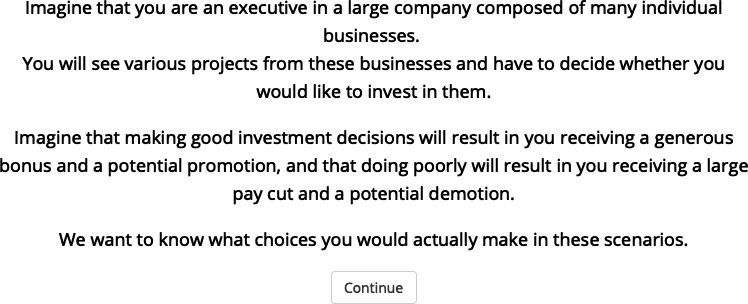
\includegraphics[width=1\linewidth]{thesis_files/figure-latex/instructions-materials-aggregation-1-1} \caption{Experiment 1 instructions.}\label{fig:instructions-materials-aggregation-1}
\end{figure}

\hypertarget{outcome-distribution-materials-aggregation-1-appendix}{%
\paragraph{Outcome distribution decision}\label{outcome-distribution-materials-aggregation-1-appendix}}

Figure~\ref{fig:project-choice-aggregated-aggregation-1} shows the outcome
distribution display that participants saw in Experiment 1.



\begin{figure}
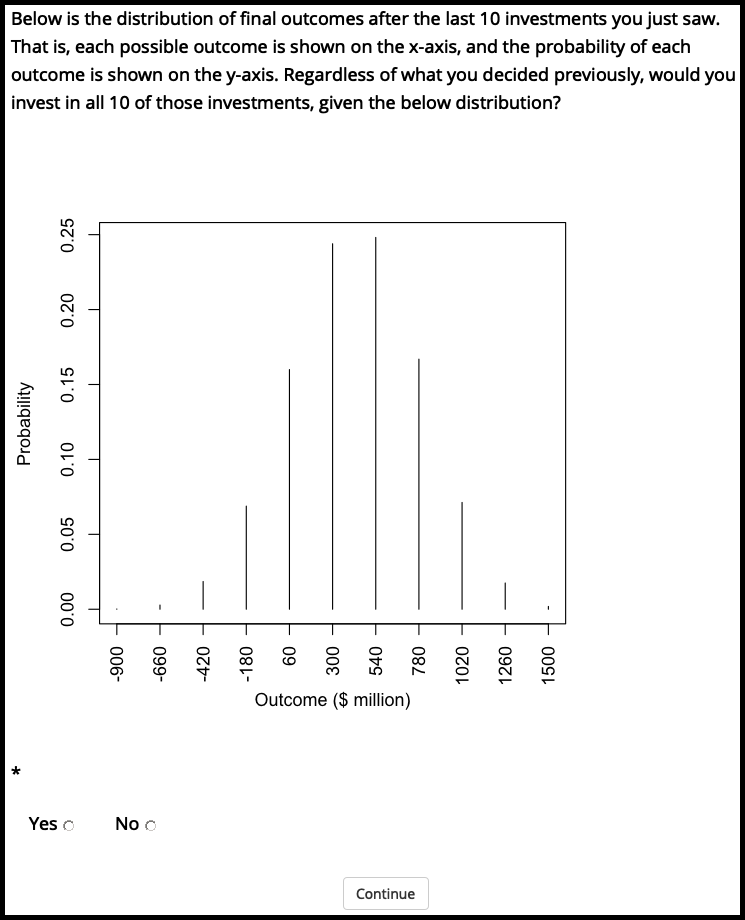
\includegraphics[width=1\linewidth]{thesis_files/figure-latex/project-choice-aggregated-aggregation-1-1} \caption{The outcome distribution of the 10 gambles used in Experiment 1.}\label{fig:project-choice-aggregated-aggregation-1}
\end{figure}

\hypertarget{follow-up-materials-aggregation-1-appendix}{%
\paragraph{Follow-up gambles}\label{follow-up-materials-aggregation-1-appendix}}

\hypertarget{negative-ev-gambles}{%
\subparagraph{Negative EV gambles}\label{negative-ev-gambles}}

I wanted to make sure that participants were generally making decisions that
were in line with EV theory and that the sample was not abnormally risk
tolerant. As such, I presented participants two project decisions that had a
negative EV. Out of the 396 negative EV
gambles included (two per participant), all but
four were rejected.

\hypertarget{samuelson1963-gambles}{%
\subparagraph{\texorpdfstring{\textcite{samuelson1963} gambles}{Samuelson (1963) gambles}}\label{samuelson1963-gambles}}

I showed participants the original \textcite{samuelson1963} gamble, asked them whether
they would accept 10 of that gamble, and whether they would accept those 10
given the associated outcome distribution. I then showed them the same three
questions, but using outcome magnitudes that were similar to the ones in the
risky investment task. That is, instead of \$100, \$100 million.

\hypertarget{redelmeier1992-gambles}{%
\subparagraph{\texorpdfstring{\textcite{redelmeier1992} gambles}{Redelmeier \& Tversky (1992) gambles}}\label{redelmeier1992-gambles}}

I then showed participants the same three types of gambles (single, 10, and
aggregated), but with the values from the gambles that were used by
\textcite{redelmeier1992}.

\hypertarget{results-aggregation-1-appendix}{%
\subsection{Results}\label{results-aggregation-1-appendix}}

\hypertarget{trial-by-trial-aggregation-1}{%
\subsubsection{Trial-by-trial analysis}\label{trial-by-trial-aggregation-1}}

Figure~\ref{fig:plot-aggregation-1-trials} shows proportions of project
acceptance across all conditions and trials.



\begin{figure}
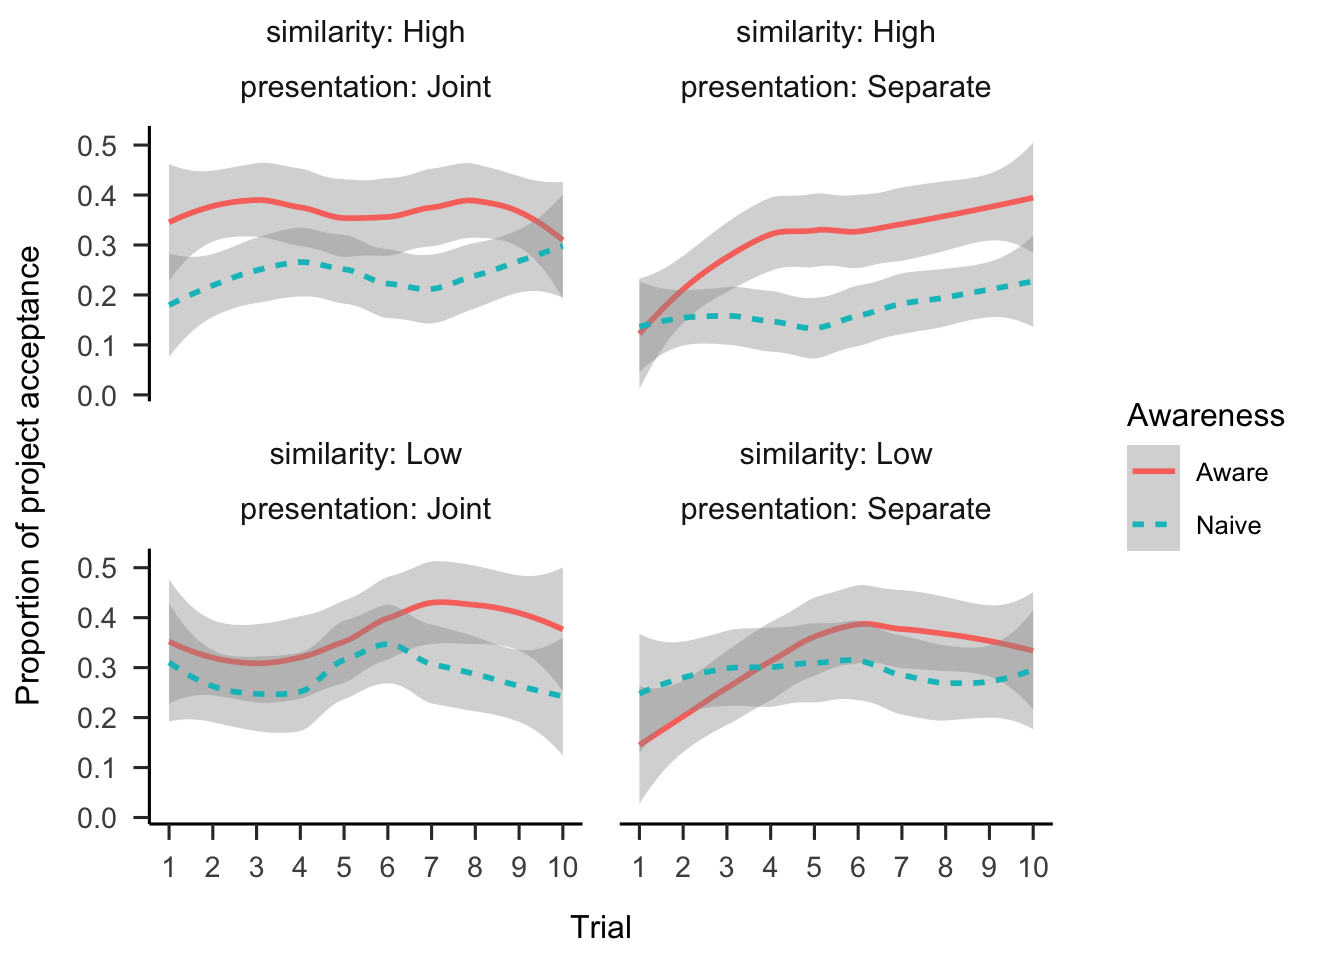
\includegraphics[width=1\linewidth]{thesis_files/figure-latex/plot-aggregation-1-trials-1} \caption{Proportion of project acceptance by trial, similarity, awareness, and presentation conditions. LOESS is used for smoothing over trials, and the shading represents 95\% confidence intervals.}\label{fig:plot-aggregation-1-trials}
\end{figure}

\hypertarget{outcome-distribution-aggregation-1}{%
\subsubsection{Outcome distribution}\label{outcome-distribution-aggregation-1}}

A paired-samples t-test was conducted to compare participants' decision to
invest in the 10 projects while seeing an aggregated distribution, and their
decisions to invest in the projects individually, without the distribution.
Participants invested in the 10 projects more when seeing the distribution both
in the separate presentation phase,
\(t(197) = 5.48\), \(p < .001\), \(d_z = 0.50\), 95\% CI \([0.31, 0.68]\); and in the joint
presentation phase, \(t(197) = 4.17\), \(p < .001\), \(d_z = 0.37\), 95\% CI \([0.19, 0.56]\).

However, I subsequently discovered that the code that generated this
distribution mistakenly flipped the outcome values. This means that although it
appeared from the distribution that the propability of loss was
0.09, the actual probability of loss of the
underlying values given the correct distribution was
0.26. As such, even though I found an
effect of distribution, it is unclear if the effect was driven by participants
actually accurately assessing the riskiness of the individual gambles, and
therefore showing a difference between the isolated and aggregated gambles in a
normative way.

\hypertarget{discussion-aggregation-1-appendix}{%
\subsection{Discussion}\label{discussion-aggregation-1-appendix}}

\hypertarget{experiment-2-1}{%
\section{Experiment 2}\label{experiment-2-1}}

\hypertarget{method-7}{%
\subsection{Method}\label{method-7}}

\hypertarget{participants-8}{%
\subsubsection{Participants}\label{participants-8}}

\hypertarget{materials-6}{%
\subsubsection{Materials}\label{materials-6}}

\hypertarget{follow-up-materials-aggregation-2-appendix}{%
\paragraph{Follow-up}\label{follow-up-materials-aggregation-2-appendix}}

Figure~\ref{fig:project-number-aggregation-2} shows the project number
question (maximum value was set to 20).
Figures~\ref{fig:portfolio-binary-aggregation-2}
and~\ref{fig:portfolio-number-aggregation-2} ask participants whether they are
willing to take all or none of the projects; and how many projects would they
choose if they could pick randomly (maximum value was set to 20). Those in the
distribution absent condition were asked the same questions, but without the
distribution and its explanation.



\begin{figure}
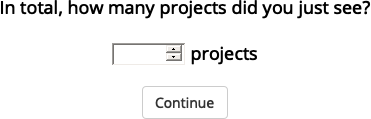
\includegraphics[width=0.5\linewidth]{thesis_files/figure-latex/project-number-aggregation-2-1} \caption{Experiment 2 project number question.}\label{fig:project-number-aggregation-2}
\end{figure}



\begin{figure}
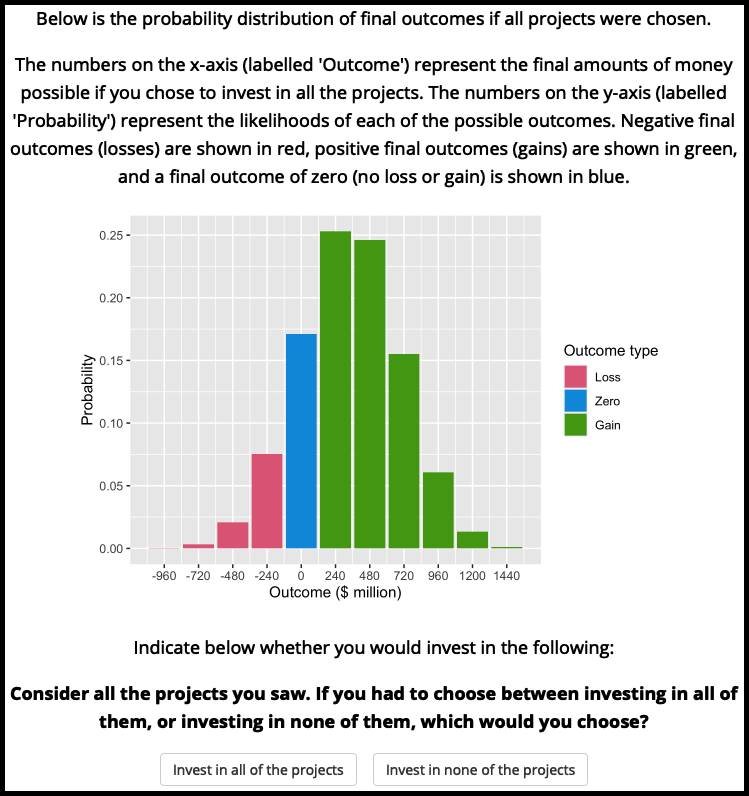
\includegraphics[width=1\linewidth]{thesis_files/figure-latex/portfolio-binary-aggregation-2-1} \caption{Experiment 2 binary portfolio question.}\label{fig:portfolio-binary-aggregation-2}
\end{figure}



\begin{figure}
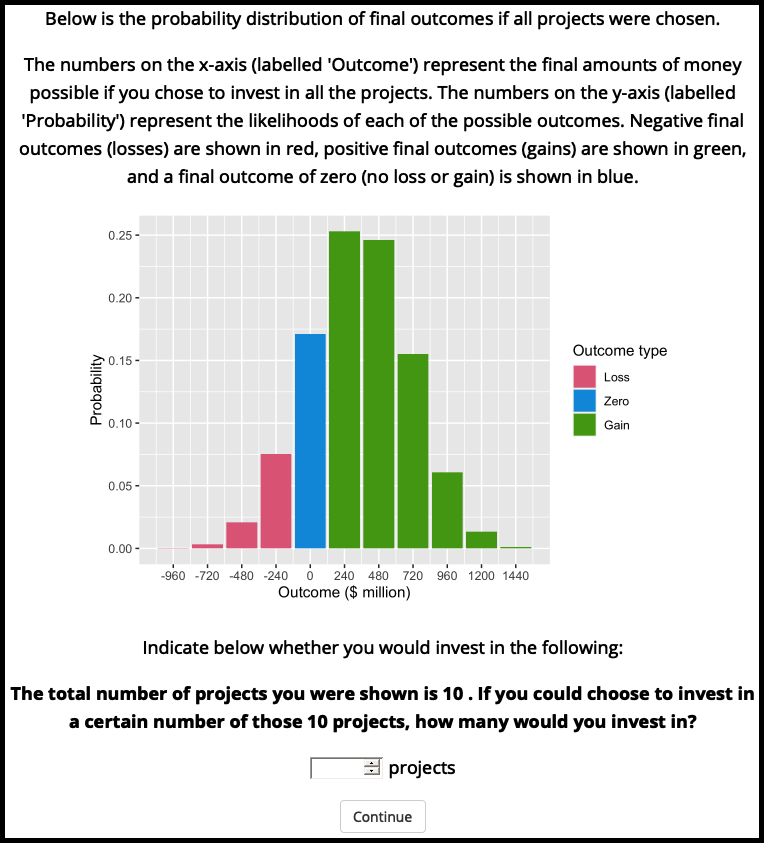
\includegraphics[width=1\linewidth]{thesis_files/figure-latex/portfolio-number-aggregation-2-1} \caption{Experiment 2 numerical portfolio question.}\label{fig:portfolio-number-aggregation-2}
\end{figure}

\hypertarget{procedure-5}{%
\subsubsection{Procedure}\label{procedure-5}}

Participants responded to demographic questions, read the instructions, and
completed the risky investment task in their respective conditions. After seeing
the individual projects, participants were then asked the three follow-up
questions.

\hypertarget{results-aggregation-2-appendix}{%
\subsection{Results}\label{results-aggregation-2-appendix}}

\hypertarget{follow-up-1}{%
\subsubsection{Follow-up}\label{follow-up-1}}

\hypertarget{project-number}{%
\paragraph{Project number}\label{project-number}}

We asked participants how many projects they think they saw.
Figure~\ref{fig:plot-aggregation-2-project-number} shows that overall people
to correctly estimate the number of projects, with more accuracy for those in
the aware condition.



\begin{figure}
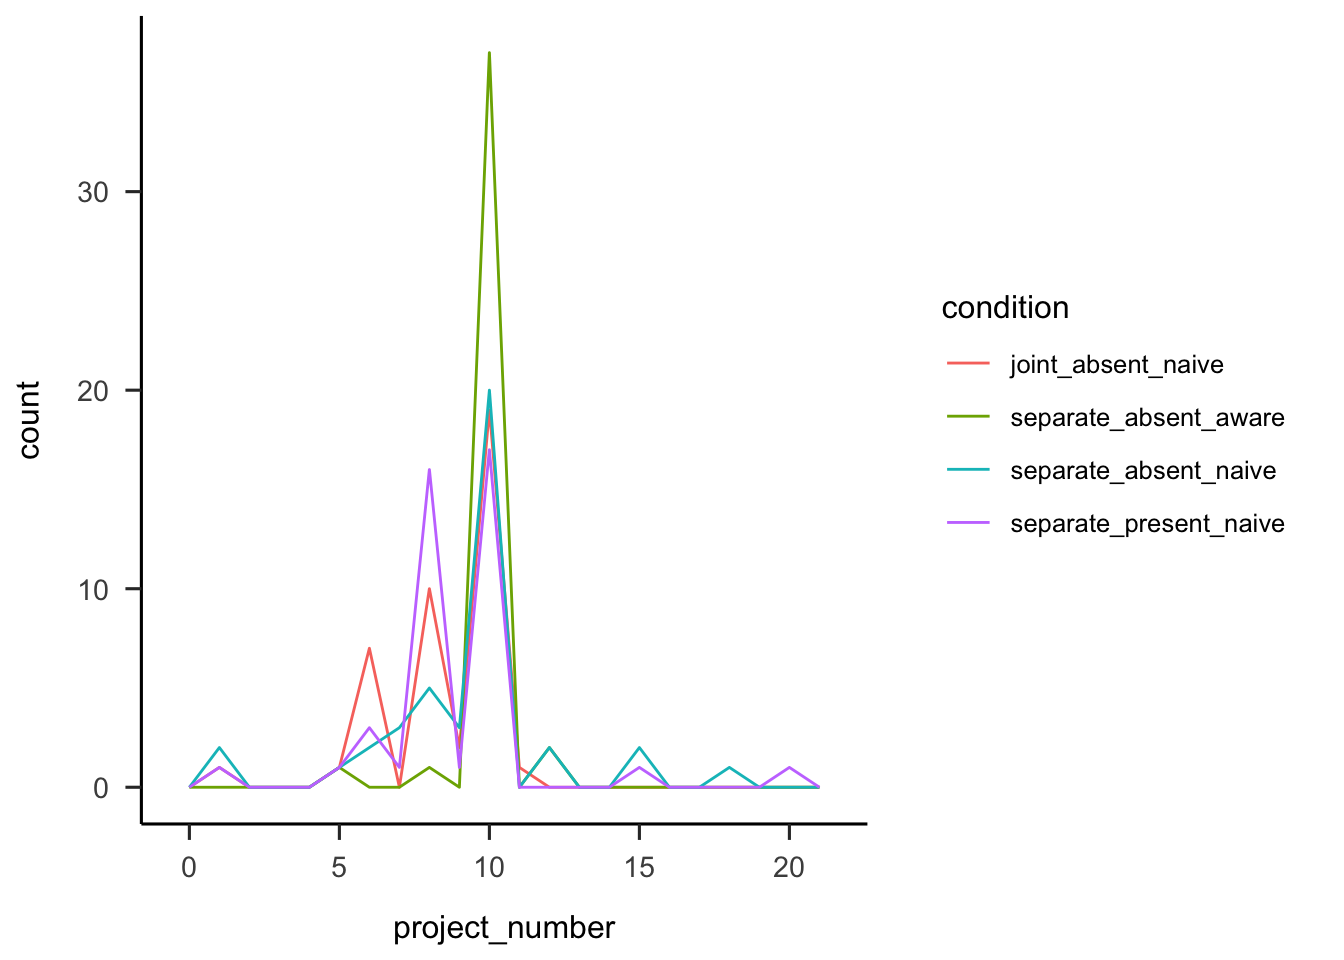
\includegraphics[width=1\linewidth]{thesis_files/figure-latex/plot-aggregation-2-project-number-1} \caption{Number of projects participants reported seeing, by condition.}\label{fig:plot-aggregation-2-project-number}
\end{figure}

\hypertarget{portfolio-choice---binary}{%
\paragraph{Portfolio choice - binary}\label{portfolio-choice---binary}}

Participants were then asked if they would rather invest in all or none of the
projects. As Figure~\ref{fig:plot-aggregation-2-portfolio-binary} shows, the
difference between presentation conditions was not significant,
\(\hat{\beta} = -0.30\), 95\% CI \([-1.19, 0.58]\), \(z = -0.67\), \(p = .500\). The
awareness effect was also not significant,
\(\hat{\beta} = -0.60\), 95\% CI \([-1.48, 0.28]\), \(z = -1.33\), \(p = .184\). However,
those that that saw a distribution chose to invest in all 10 projects
significantly more
(71.43\%) than
those that did not see a distribution
(36.59\%),
\(OR = 4.33\), 95\% CI \([1.76, 11.24]\), \(z = 3.11\), \(p = .002\).



\begin{figure}
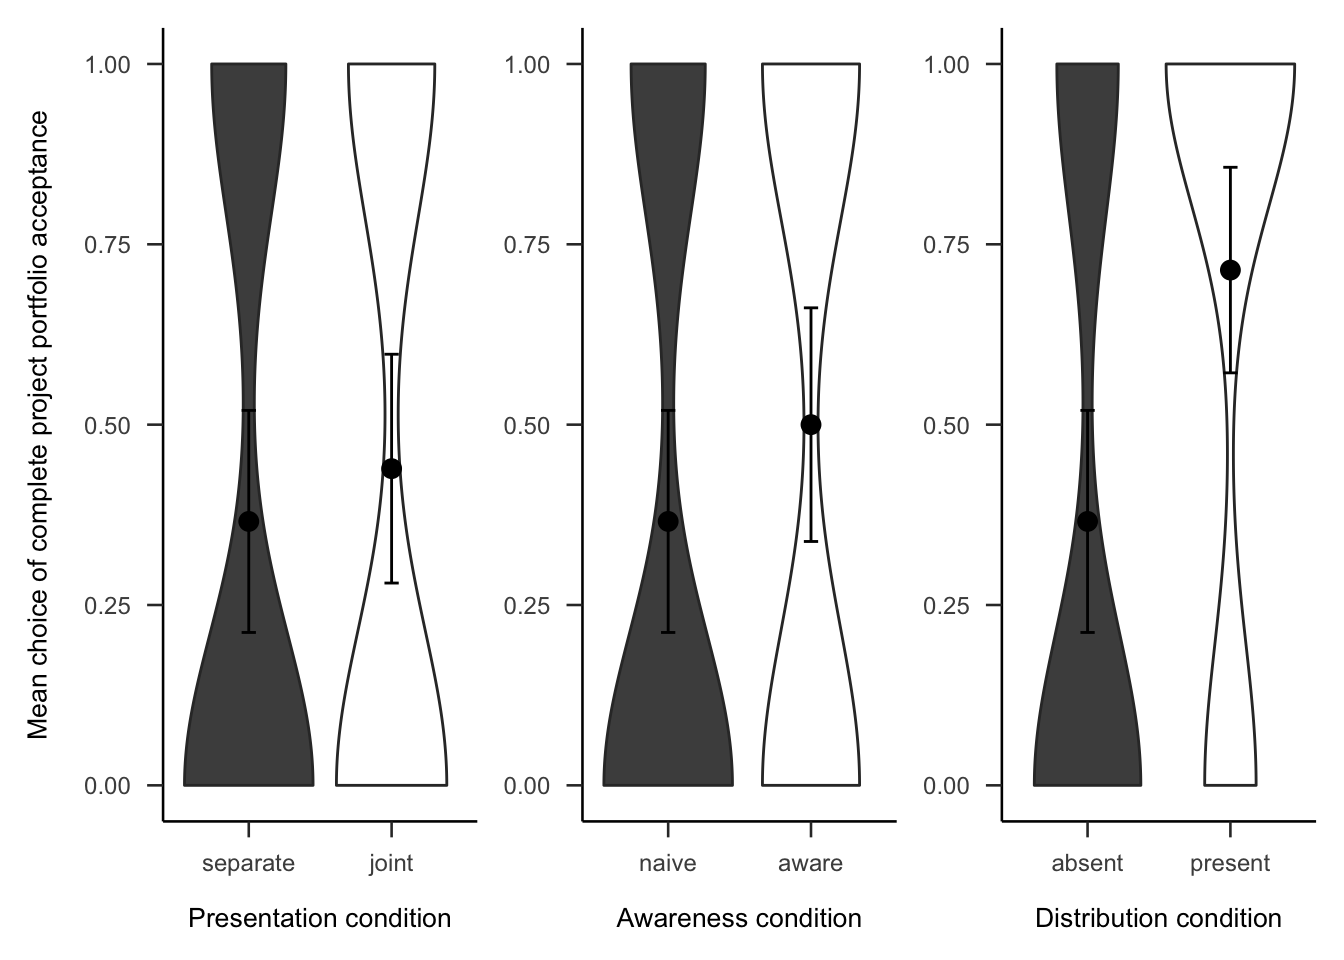
\includegraphics[width=1\linewidth]{thesis_files/figure-latex/plot-aggregation-2-portfolio-binary-1} \caption{Mean choice of investing in all 10 projects for the presentation, awareness, and distribution effects. Note, the condition on the left of each effect is the reference condition (separate presentation, naive awareness, distribution absent). As such, it is identical for the three effects.}\label{fig:plot-aggregation-2-portfolio-binary}
\end{figure}

\hypertarget{portfolio-choice---number}{%
\paragraph{Portfolio choice - number}\label{portfolio-choice---number}}

Subsequently, we asked participants how many projects they would invest in out
of the 10 that they saw. As
Figure~\ref{fig:plot-aggregation-2-portfolio-number} shows, the difference
between presentation conditions was not significant,
\(d_s\) = 0.08, 95\% CI {[}-0.35, 0.52{]}, \(t\)(80) = 0.38, \(p\) = .706. The awareness effect
was also not significant, \(d_s\) = 0.13, 95\% CI {[}-0.31, 0.56{]}, \(t\)(80) = 0.57, \(p\) = .570.
However, those that that saw a distribution chose to invest in significantly
more projects than those that did not see a distribution,
\(d_s\) = 0.60, 95\% CI {[}0.15, 1.03{]}, \(t\)(81) = 2.70, \(p\) = .009.



\begin{figure}
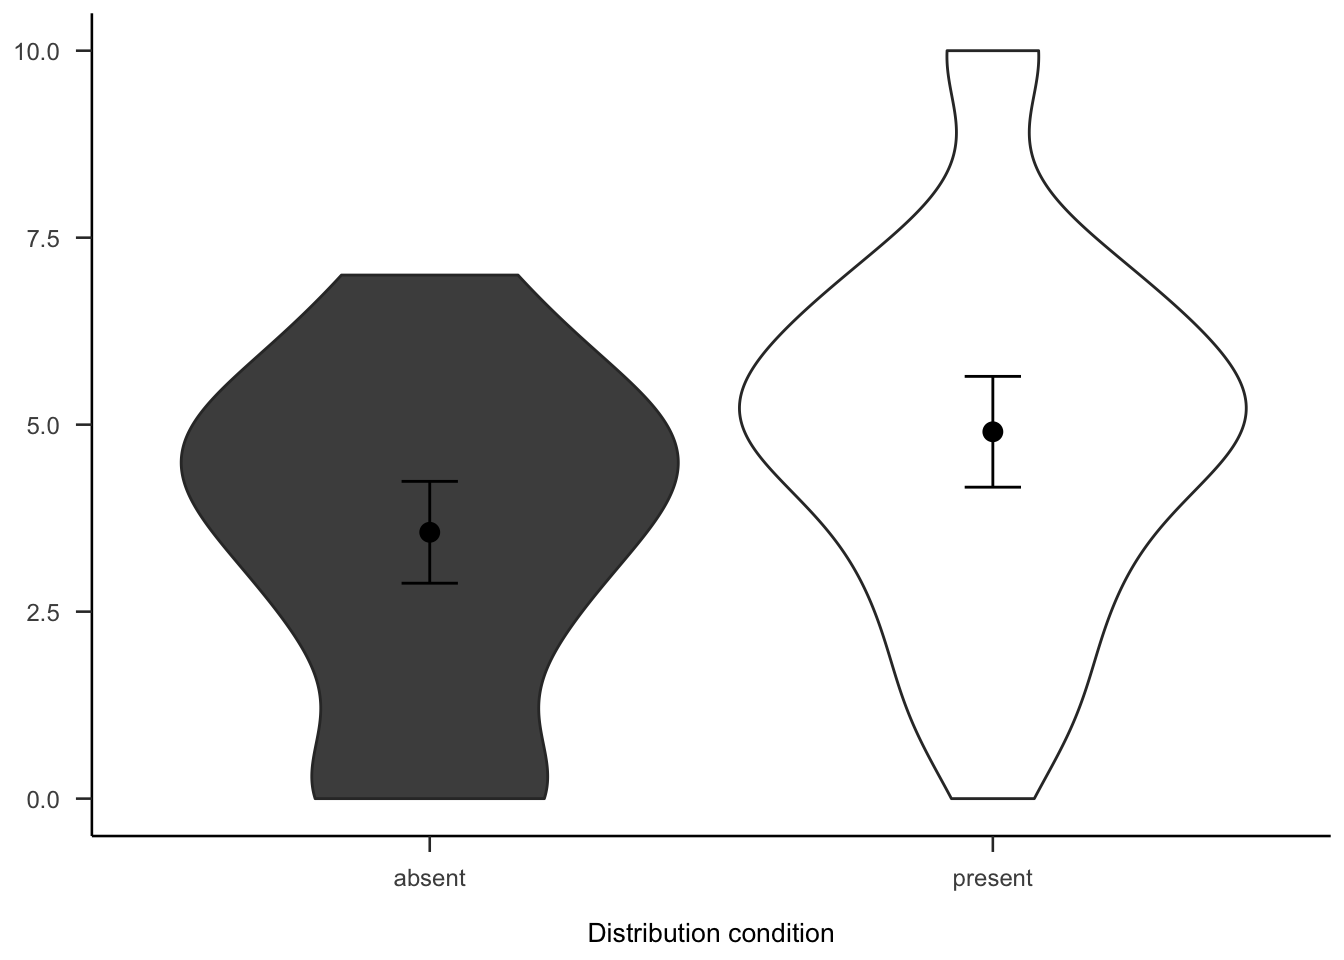
\includegraphics[width=1\linewidth]{thesis_files/figure-latex/plot-aggregation-2-portfolio-number-1} \caption{Mean number of projects chosen in the follow-up for the presentation, awareness, and distribution effects. Note, the condition on the left of each effect is the reference condition (separate presentation, naive awareness, distribution absent). As such, it is identical for the three effects.}\label{fig:plot-aggregation-2-portfolio-number}
\end{figure}

\hypertarget{gambles}{%
\subsubsection{Gambles}\label{gambles}}

Figures~\ref{fig:plot-aggregation-2-trials}
and~\ref{fig:plot-aggregation-2-gamble-values} show the overall people seemed
to prefer gambles with higher probabilities of gain, sometimes regardless of
expected value or value of the gain.



\begin{figure}
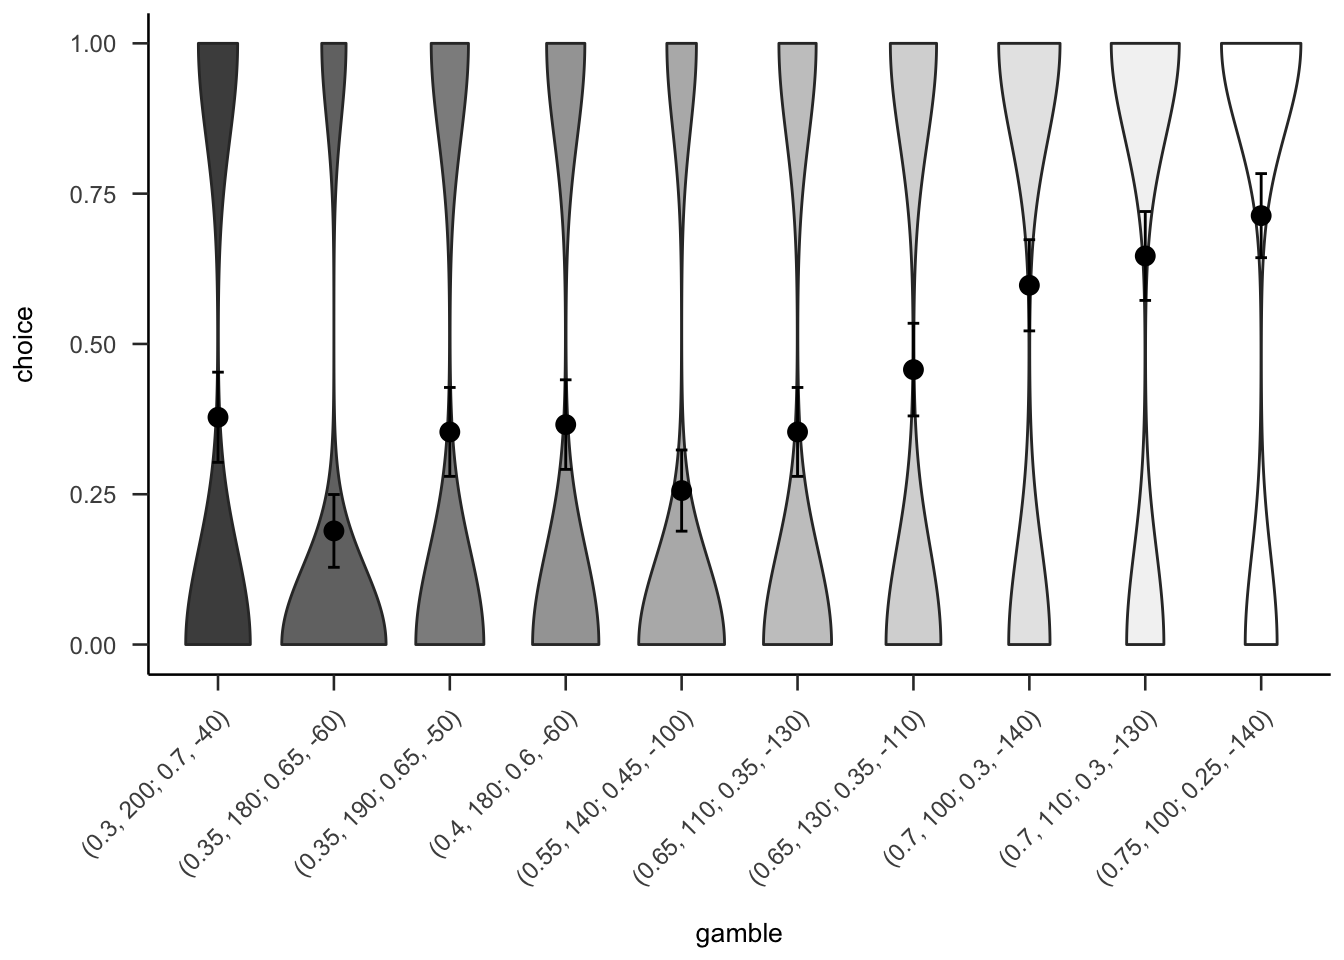
\includegraphics[width=1\linewidth]{thesis_files/figure-latex/plot-aggregation-2-trials-1} \caption{Mean project acceptance for the 10 gambles. The format of the labels indicate: (gain probability, gain value; loss probability, loss value).}\label{fig:plot-aggregation-2-trials}
\end{figure}



\begin{figure}
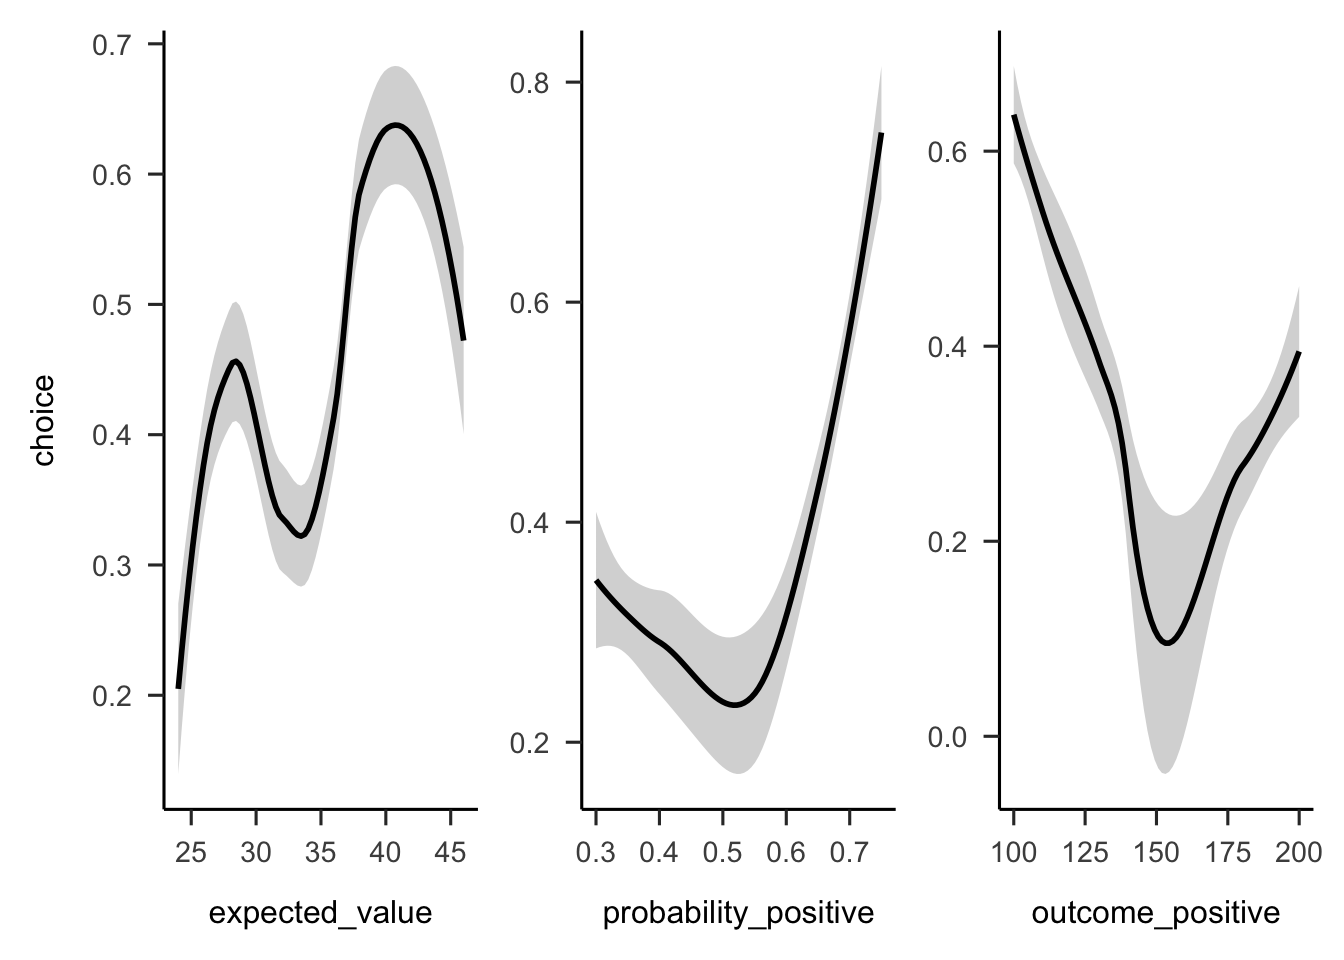
\includegraphics[width=1\linewidth]{thesis_files/figure-latex/plot-aggregation-2-gamble-values-1} \caption{Mean project acceptance for the gambles' expected value, positive probability, and positive outcome.}\label{fig:plot-aggregation-2-gamble-values}
\end{figure}

\hypertarget{discussion-6}{%
\subsection{Discussion}\label{discussion-6}}

\hypertarget{aggregation-3}{%
\section{Experiment 3}\label{aggregation-3}}

Experiment 3 investigated the effect of similarity on project choice. The
previous experiments did not counterbalance the project domain when displaying
the 10 projects to participants. In Experiment 3, I used 10 different potential
business domains when constructing the project descriptions in order to reduce
any potential effect that the specific domain may have on people's choice.

I again tested Hypothesis~\ref{hyp:similarity-aggregation-1}.

\hypertarget{method-8}{%
\subsection{Method}\label{method-8}}

\hypertarget{participants-9}{%
\subsubsection{Participants}\label{participants-9}}

Two hundred and sixty-six (127 female) people were recruited from the online recruitment platform Prolific. Participants were compensated at a rate of £5 an hour. The average age was 39.56 (\emph{SD} = 8.77, \emph{min} = 25, \emph{max} = 71). Participants reported an average of 5.64 (\emph{SD} = 6.45, \emph{min} = 0, \emph{max} = 40) years of work in a business setting, and an average of 3.28 (\emph{SD} = 4.92, \emph{min} = 0, \emph{max} = 30) years of business education. The mean completion time was 9.23 (\emph{SD} = 7.2, \emph{min} = 1.41, \emph{max} = 65.46) minutes.~Table~\ref{tab:condition-allocation-aggregation-3}
shows the between-subjects condition allocation.

\begin{table}[tbp]

\begin{center}
\begin{threeparttable}

\caption{\label{tab:condition-allocation-aggregation-3}Experiment 3 group allocation.}

\begin{tabular}{ll}
\toprule
Similarity & \multicolumn{1}{c}{N}\\
\midrule
High & 133\\
Low & 133\\
Total & 266\\
\bottomrule
\end{tabular}

\end{threeparttable}
\end{center}

\end{table}

\hypertarget{materials-7}{%
\subsubsection{Materials}\label{materials-7}}

\hypertarget{instructions-5}{%
\paragraph{Instructions}\label{instructions-5}}

Participants were shown the same instructions as in
\protect\hyperlink{instructions-materials-aggregation-1}{Experiment 1}.

\hypertarget{task-aggregation-3}{%
\paragraph{Risky investment task}\label{task-aggregation-3}}

Participants saw displays with the same gamble values as those in
\protect\hyperlink{task-aggregation-2}{Experiment 2}, but with some changes in wording and
sentence structure. I kept the same gamble information, but added extra prose
describing the projects and randomised the order of the sentences, so that the
descriptions would not appear so similar. See
Figure~\ref{fig:project-choice-aggregation-3} for an example.



\begin{figure}
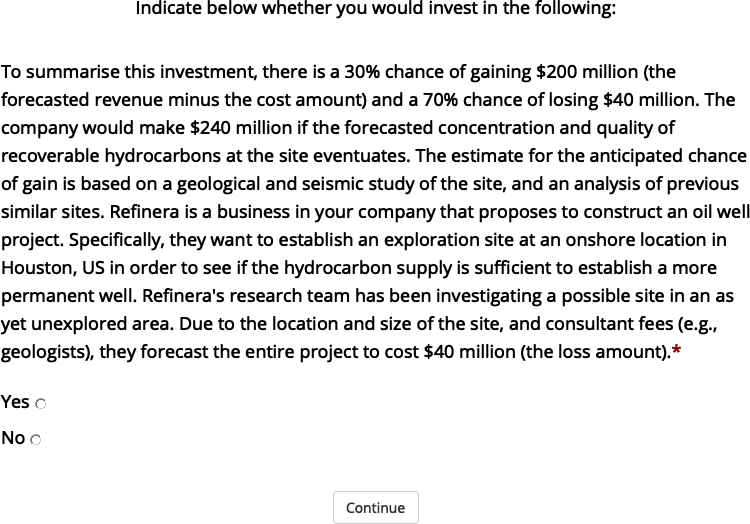
\includegraphics[width=1\linewidth]{thesis_files/figure-latex/project-choice-aggregation-3-1} \caption{An example of a project display in Experiment 3.}\label{fig:project-choice-aggregation-3}
\end{figure}

The similarity manipulation was as in Experiment 1. However, here I varied
project domain so that in the high similarity condition participants saw one of
the ten project domains.

\hypertarget{follow-up-aggregation-3}{%
\paragraph{Follow-up}\label{follow-up-aggregation-3}}

The follow-up questions were similar to those in
\protect\hyperlink{follow-up-aggregation-2}{Experiment 2}, except in the portfolio number
question I added the number of projects that they saw (10). Further, I added a
question asking how many projects participants were expecting to see at the
beginning of the experiment (see
Figure~\ref{fig:project-expectation-aggregation-3}).



\begin{figure}

\includegraphics[width=1\linewidth]{thesis_files/figure-latex/project-expectation-aggregation-3-1} \caption{Experiment 3 project expectation question.}\label{fig:project-expectation-aggregation-3}
\end{figure}

\hypertarget{procedure-6}{%
\subsubsection{Procedure}\label{procedure-6}}

Participants responded to demographic questions, read the instructions, and
completed the risky investment task in their respective conditions. After seeing
the individual projects, participants were then asked the four follow-up
questions.

\hypertarget{results-4}{%
\subsection{Results}\label{results-4}}

\hypertarget{project-investment-1}{%
\subsubsection{Project investment}\label{project-investment-1}}

The project investment data was analysed as in
\protect\hyperlink{results-aggregation-2}{Experiment 2}.
Figures~\ref{fig:plot-aggregation-3-choice}
and~\ref{fig:plot-aggregation-3-proportion} show the choice and proportion
data, respectively. The difference between similarity conditions was not
significant, both in the logistic regression
\(b = 0.01\), 95\% CI \([-0.34, 0.36]\), \(z = 0.04\), \(p = .966\), and in the t-test,
\(d_s\) = -0.21, 95\% CI {[}-0.45, 0.03{]}, \(t\)(264) = -1.69, \(p\) = .093.



\begin{figure}
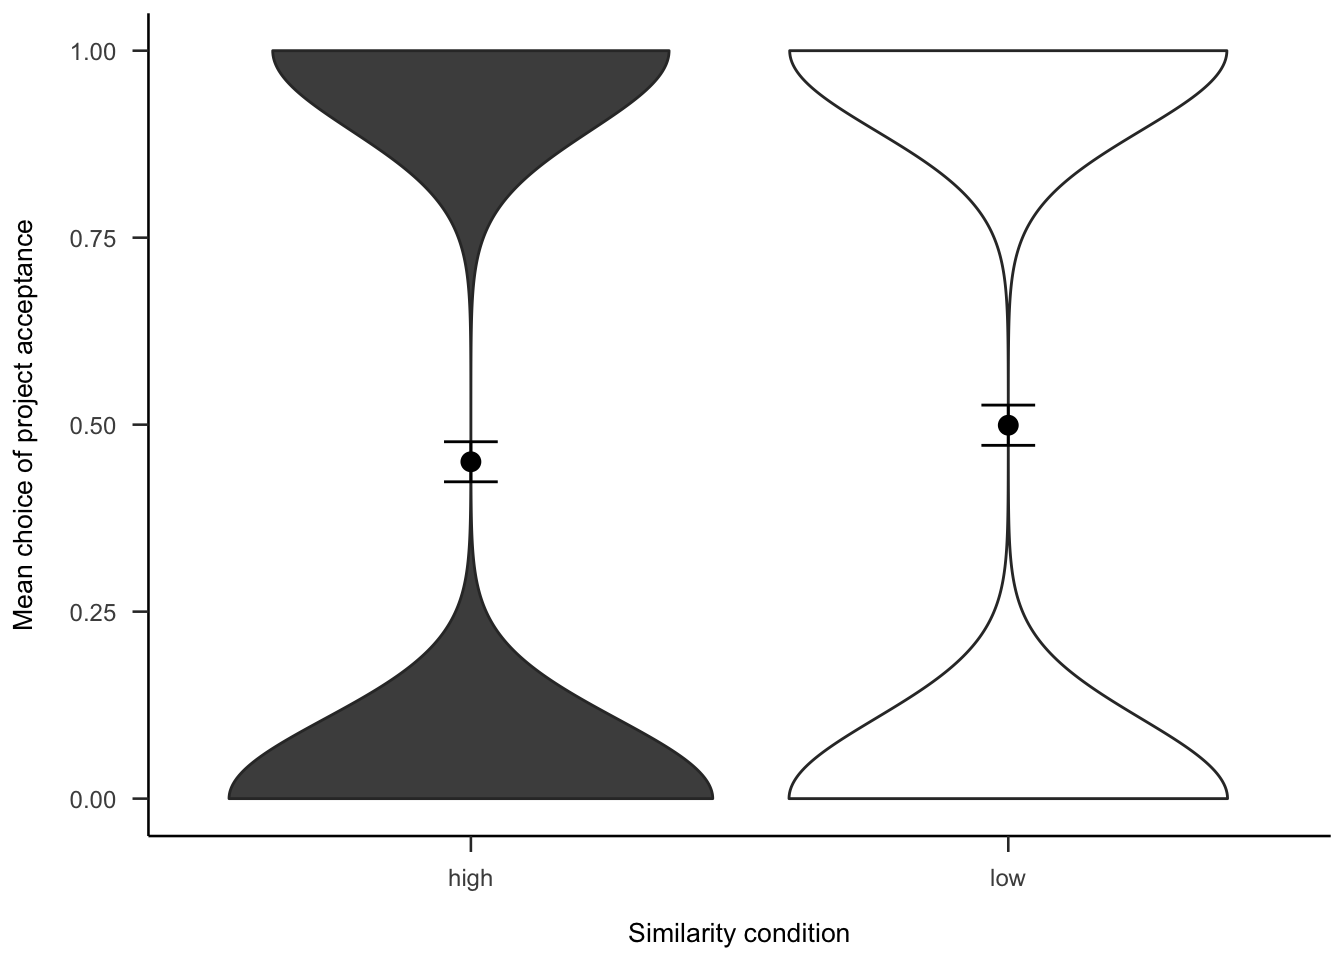
\includegraphics[width=1\linewidth]{thesis_files/figure-latex/plot-aggregation-3-choice-1} \caption{Mean project acceptance for the similarity effect.}\label{fig:plot-aggregation-3-choice}
\end{figure}



\begin{figure}
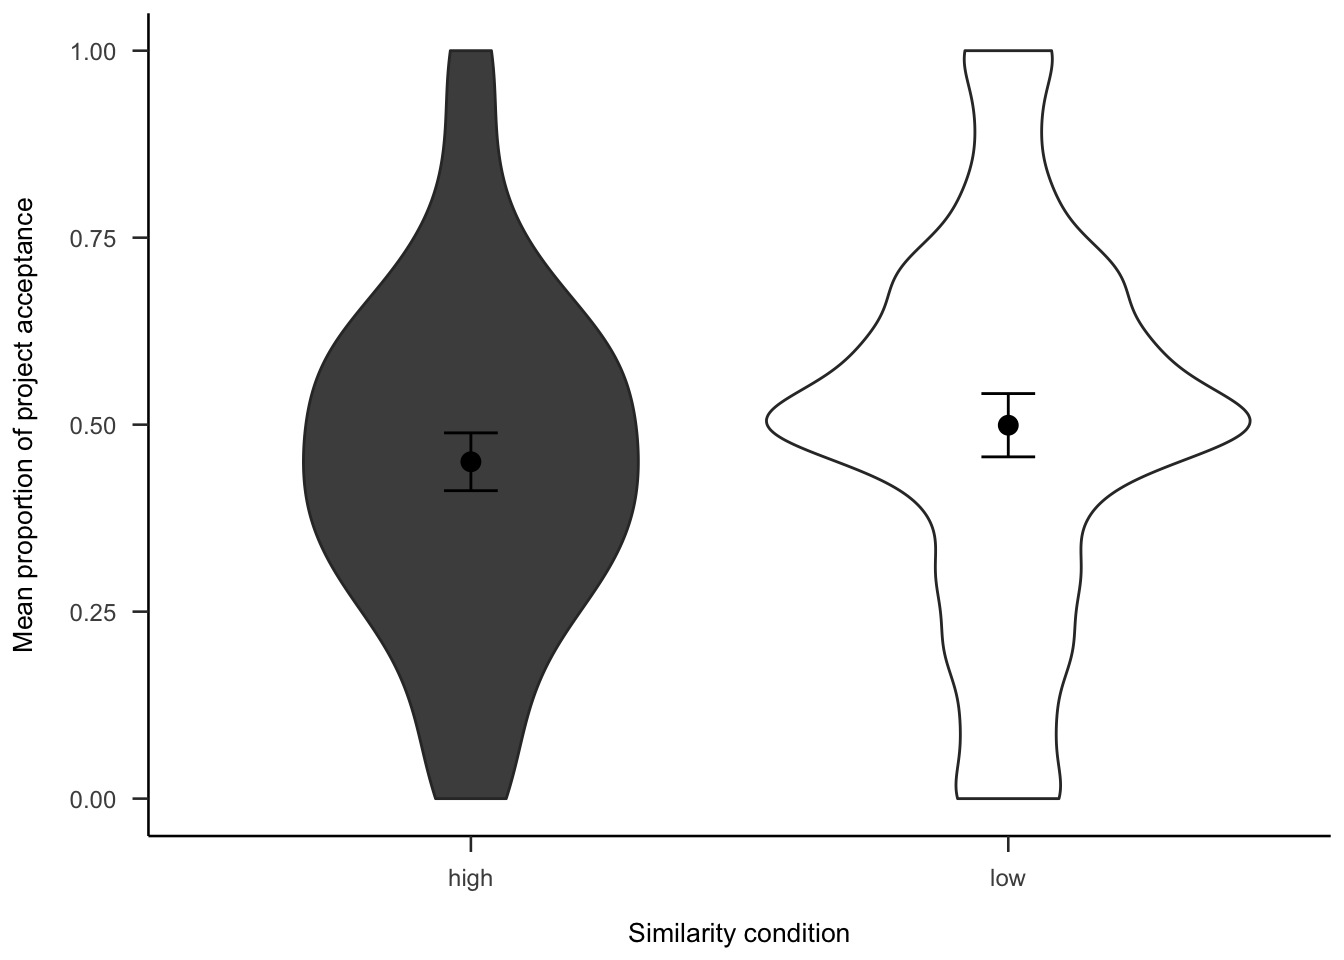
\includegraphics[width=1\linewidth]{thesis_files/figure-latex/plot-aggregation-3-proportion-1} \caption{Mean proportion of project acceptance for the similarity effect.}\label{fig:plot-aggregation-3-proportion}
\end{figure}

Further, Figure~\ref{fig:plot-aggregation-3-choice-trials} shows the choice
data as a function of the order of the project in the sequence. As
Table~\ref{tab:similarity-project-order} shows, there were no main effects or
interactions.



\begin{figure}
\includegraphics[width=1\linewidth]{thesis_files/figure-latex/plot-aggregation-3-choice-trials-1} \caption{Mean project acceptance by similarity and trial.}\label{fig:plot-aggregation-3-choice-trials}
\end{figure}

\begin{table}[tbp]

\begin{center}
\begin{threeparttable}

\caption{\label{tab:similarity-project-order}Logistic regression table of project acceptance by similarity and trial.}

\begin{tabular}{lllll}
\toprule
Term & \multicolumn{1}{c}{$\hat{\beta}$} & \multicolumn{1}{c}{95\% CI} & \multicolumn{1}{c}{$z$} & \multicolumn{1}{c}{$p$}\\
\midrule
Intercept & -0.02 & {}[-0.31, 0.28] & -0.11 & .916\\
Similaritylow & 0.05 & {}[-0.37, 0.46] & 0.22 & .826\\
Project order & -0.04 & {}[-0.08, 0.00] & -1.83 & .067\\
Similaritylow $\times$ Project order & 0.03 & {}[-0.03, 0.09] & 1.07 & .284\\
\bottomrule
\end{tabular}

\end{threeparttable}
\end{center}

\end{table}

\hypertarget{follow-up-2}{%
\subsubsection{Follow-up}\label{follow-up-2}}

\hypertarget{project-expectation}{%
\paragraph{Project expectation}\label{project-expectation}}

We asked participants how many projects they expected to see. As
Figure~\ref{fig:plot-aggregation-3-project-expectation} shows, the difference
between similarity conditions was not significant,
\(d_s\) = -0.23, 95\% CI {[}-0.47, 0.01{]}, \(t\)(264) = -1.85, \(p\) = .065.



\begin{figure}
\includegraphics[width=1\linewidth]{thesis_files/figure-latex/plot-aggregation-3-project-expectation-1} \caption{Number of projects participants expected to see, by similarity.}\label{fig:plot-aggregation-3-project-expectation}
\end{figure}

\hypertarget{project-number-1}{%
\paragraph{Project number}\label{project-number-1}}

We asked participants how many projects they think they saw.
Figure~\ref{fig:plot-aggregation-3-project-number} shows that overall people
correctly estimate the number of projects.



\begin{figure}
\includegraphics[width=1\linewidth]{thesis_files/figure-latex/plot-aggregation-3-project-number-1} \caption{Number of projects participants reported seeing, by similarity.}\label{fig:plot-aggregation-3-project-number}
\end{figure}

\hypertarget{portfolio-choice---binary-1}{%
\paragraph{Portfolio choice - binary}\label{portfolio-choice---binary-1}}

Participants were then asked if they would rather invest in all or none of the
projects. As Figure~\ref{fig:plot-aggregation-3-portfolio-binary} shows, those
in the low similarity condition were significantly more likely to want to invest
in all of the projects,
\(b = 0.52\), 95\% CI \([0.04, 1.02]\), \(z = 2.10\), \(p = .036\).



\begin{figure}
\includegraphics[width=1\linewidth]{thesis_files/figure-latex/plot-aggregation-3-portfolio-binary-1} \caption{Mean choice of investing in all 10 projects for the similarity effect.}\label{fig:plot-aggregation-3-portfolio-binary}
\end{figure}

\hypertarget{portfolio-choice---number-1}{%
\paragraph{Portfolio choice - number}\label{portfolio-choice---number-1}}

Subsequently, we asked participants how many projects they would invest in out
of the 10 that they saw. As
Figure~\ref{fig:plot-aggregation-3-portfolio-number} shows, the difference
between similarity conditions was not significant,
\(d_s\) = -0.14, 95\% CI {[}-0.38, 0.10{]}, \(t\)(264) = -1.12, \(p\) = .264.



\begin{figure}
\includegraphics[width=1\linewidth]{thesis_files/figure-latex/plot-aggregation-3-portfolio-number-1} \caption{Mean number of projects chosen in the follow-up for the similarity effect.}\label{fig:plot-aggregation-3-portfolio-number}
\end{figure}

\hypertarget{gambles-1}{%
\subsubsection{Gambles}\label{gambles-1}}

Figures~\ref{fig:plot-aggregation-3-trials}
and~\ref{fig:plot-aggregation-3-gamble-values} show the
overall people seemed to prefer gambles with higher probabilities of gain,
sometimes regardless of expected value or value of the gain.



\begin{figure}
\includegraphics[width=1\linewidth]{thesis_files/figure-latex/plot-aggregation-3-trials-1} \caption{Mean project acceptance for the 10 gambles. The format of the labels indicate: (gain probability, gain value; loss probability, loss value).}\label{fig:plot-aggregation-3-trials}
\end{figure}




\begin{figure}
\includegraphics[width=1\linewidth]{thesis_files/figure-latex/plot-aggregation-3-gamble-values-1} \caption{Mean project acceptance for the gambles'
expected value, positive probability, and positive outcome.}\label{fig:plot-aggregation-3-gamble-values}
\end{figure}

\hypertarget{discussion-7}{%
\subsection{Discussion}\label{discussion-7}}

I found some evidence for the effect of similarity on project choice, but it was
in the opposite direction to the one hypothesised. Specifically, I found that
when considering projects individually, participants' risk aversion did not
differ between similarity conditions, but when offered a portfolio of the
projects, those that saw the dissimilar projects were more likely to invest.

These results provide evidence for the naive diversification account expressed
\protect\hyperlink{similarity-discussion-aggregation-1}{above}. Specifically, it may be the case
that participants really are naively diversifying, but only when they are
explicitly given an opportunity to do so. This is similar to the multi-play
effects in that the question itself provides a sort of choice bracketing. That
is, the gambles are grouped together as a package/portfolio by the question.
Together, this suggests that people are not naively aggregating when viewing
gambles in isolation, but when the choices are bracketed explicitly, then the
choice seems to be driven by a naive diversification.

\hypertarget{aggregation-4}{%
\section{Experiment 4}\label{aggregation-4}}

Experiment 4 investigated the effect of ``awareness'' on project choice. In
Experiment 1 we found an effect of awareness in the trial-by-trial data that was
not replicated in Experiment 2. Previously, I explained this effect using the
law of small numbers; people may have been anticipating less risky gambles
towards the end of the set. As such, it might be the case that the effect will
be seen with more trials. In Experiment 4 we attempted to replicate the effect
from Experiment 1 with 20 projects. The ``naive'' condition attempted to encourage
participants to focus on projects one at a time and did not say how many
projects there were. The ``aware'' condition attempted to encourage participants
to think of all 20 projects (by saying the total number in the beginning, and
notifying participants where they were in the project order).

I again tested Hypothesis~\ref{hyp:awareness-trials-aggregation-2}.

\hypertarget{method-9}{%
\subsection{Method}\label{method-9}}

\hypertarget{participants-10}{%
\subsubsection{Participants}\label{participants-10}}

Two hundred and sixty-six (110 female) people were recruited from the online recruitment platform Prolific. Participants were compensated at a rate of £5 an hour. The average age was 40.62 (\emph{SD} = 9.59, \emph{min} = 25, \emph{max} = 74). Participants reported an average of 7.45 (\emph{SD} = 7.8, \emph{min} = 0, \emph{max} = 47) years of work in a business setting, and an average of 5.52 (\emph{SD} = 7.27, \emph{min} = 0, \emph{max} = 48) years of business education. The mean completion time was 12.66 (\emph{SD} = 8.26, \emph{min} = 1.48, \emph{max} = 53.47) minutes.~Table~\ref{tab:condition-allocation-aggregation-4}
shows the between-subjects condition allocation.

\begin{table}[tbp]

\begin{center}
\begin{threeparttable}

\caption{\label{tab:condition-allocation-aggregation-4}Experiment 4 group allocation.}

\begin{tabular}{ll}
\toprule
Awareness & \multicolumn{1}{c}{N}\\
\midrule
Aware & 133\\
Naive & 133\\
Total & 266\\
\bottomrule
\end{tabular}

\end{threeparttable}
\end{center}

\end{table}

\hypertarget{materials-8}{%
\subsubsection{Materials}\label{materials-8}}

\hypertarget{instructions-6}{%
\paragraph{Instructions}\label{instructions-6}}

Participants were shown similar instructions as in
\protect\hyperlink{instructions-materials-aggregation-1}{Experiment 1}, except that the awareness
manipulation was incorporated into the text. Participants in the naive condition
saw the instructions in Figure~\ref{fig:instructions-naive-aggregation-4}, and
those in the aware condition saw the instructions in
Figure~\ref{fig:instructions-aware-aggregation-4}.



\begin{figure}
\includegraphics[width=1\linewidth]{thesis_files/figure-latex/instructions-naive-aggregation-4-1} \caption{Instructions for those in the naive condition of Experiment 4.}\label{fig:instructions-naive-aggregation-4}
\end{figure}



\begin{figure}
\includegraphics[width=1\linewidth]{thesis_files/figure-latex/instructions-aware-aggregation-4-1} \caption{Instructions for those in the aware condition of Experiment 4.}\label{fig:instructions-aware-aggregation-4}
\end{figure}

\hypertarget{risky-investment-task}{%
\paragraph{Risky investment task}\label{risky-investment-task}}

Participants saw similar displays to those in
\protect\hyperlink{task-aggregation-3}{Experiment 3}. However, here participants viewed 20
projects, so while the gamble constrains explained above were still applied, the
actual gamble values were different. Further, those in the aware condition saw
an added sentence that identified the number of the project they were currently
considering in the context of the total 20. See
Figure~\ref{fig:project-choice-aggregation-4} for an example. Those in the
naive condition saw the same display without this sentence.



\begin{figure}
\includegraphics[width=1\linewidth]{thesis_files/figure-latex/project-choice-aggregation-4-1} \caption{An example of a project display in Experiment 4.}\label{fig:project-choice-aggregation-4}
\end{figure}

\hypertarget{follow-up-3}{%
\paragraph{Follow-up}\label{follow-up-3}}

The follow-up questions were identical to those in
\protect\hyperlink{follow-up-aggregation-3}{Experiment 3}, except that the portfolio number
question identified the number of projects they saw as 20.

\hypertarget{procedure-7}{%
\subsubsection{Procedure}\label{procedure-7}}

Participants responded to demographic questions, read the instructions, and
completed the risky investment task in their respective conditions. After seeing
the individual projects, participants were then asked the four follow-up
questions.

\hypertarget{results-5}{%
\subsection{Results}\label{results-5}}

\hypertarget{project-investment-2}{%
\subsubsection{Project investment}\label{project-investment-2}}

The project investment data was analysed as in
\protect\hyperlink{results-aggregation-2}{Experiment 2}.
Figures~\ref{fig:plot-aggregation-4-choice}
and~\ref{fig:plot-aggregation-4-proportion} show the choice and proportion
data, respectively. The difference between
awareness conditions was not significant, both in the logistic regression
\(b = 0.09\), 95\% CI \([-0.25, 0.44]\), \(z = 0.53\), \(p = .595\), and in the t-test,
\(d_s\) = -0.09, 95\% CI {[}-0.33, 0.15{]}, \(t\)(264) = -0.73, \(p\) = .464.



\begin{figure}
\includegraphics[width=1\linewidth]{thesis_files/figure-latex/plot-aggregation-4-choice-1} \caption{Mean project acceptance for the awareness effect.}\label{fig:plot-aggregation-4-choice}
\end{figure}



\begin{figure}
\includegraphics[width=1\linewidth]{thesis_files/figure-latex/plot-aggregation-4-proportion-1} \caption{Mean proportion of project acceptance for the awareness effect.}\label{fig:plot-aggregation-4-proportion}
\end{figure}

Further, Figure~\ref{fig:plot-aggregation-4-choice-trials} shows the choice
data as a function of the order of the project in the sequence. As
Table~\ref{tab:awareness-project-order} shows, there were no main effects or
interactions.



\begin{figure}
\includegraphics[width=1\linewidth]{thesis_files/figure-latex/plot-aggregation-4-choice-trials-1} \caption{Mean project acceptance by awareness and trial.}\label{fig:plot-aggregation-4-choice-trials}
\end{figure}

\begin{table}[tbp]

\begin{center}
\begin{threeparttable}

\caption{\label{tab:awareness-project-order}Logistic regression table of project acceptance by awareness and trial.}

\begin{tabular}{lllll}
\toprule
Term & \multicolumn{1}{c}{$\hat{\beta}$} & \multicolumn{1}{c}{95\% CI} & \multicolumn{1}{c}{$z$} & \multicolumn{1}{c}{$p$}\\
\midrule
Intercept & -0.11 & {}[-0.37, 0.15] & -0.82 & .410\\
Awarenessaware & 0.20 & {}[-0.17, 0.57] & 1.05 & .293\\
Project order & 0.01 & {}[0.00, 0.03] & 1.37 & .170\\
Awarenessaware $\times$ Project order & 0.00 & {}[-0.03, 0.02] & -0.29 & .775\\
\bottomrule
\end{tabular}

\end{threeparttable}
\end{center}

\end{table}

\hypertarget{follow-up-4}{%
\subsubsection{Follow-up}\label{follow-up-4}}

\hypertarget{project-expectation-1}{%
\paragraph{Project expectation}\label{project-expectation-1}}

We asked participants how many projects they expected to see.
Figure~\ref{fig:plot-aggregation-4-project-expectation} shows that those in
the aware condition reportedly expect to see more,
\(d_s\) = -0.94, 95\% CI {[}-1.19, -0.69{]}, \(t\)(264) = -7.67, \(p\) \textless{} .001. However, this is likely to be due to
the fact that they were told how many projects there were.



\begin{figure}
\includegraphics[width=1\linewidth]{thesis_files/figure-latex/plot-aggregation-4-project-expectation-1} \caption{Number of projects participants expected to see, by awareness.}\label{fig:plot-aggregation-4-project-expectation}
\end{figure}

\hypertarget{project-number-2}{%
\paragraph{Project number}\label{project-number-2}}

We asked participants how many projects they think they saw.
Figure~\ref{fig:plot-aggregation-4-project-number} shows that overall people
correctly estimate the number of projects, with higher accuracy for those in the
aware condition.



\begin{figure}
\includegraphics[width=1\linewidth]{thesis_files/figure-latex/plot-aggregation-4-project-number-1} \caption{Number of projects participants reported seeing, by awareness.}\label{fig:plot-aggregation-4-project-number}
\end{figure}

\hypertarget{portfolio-choice---binary-2}{%
\paragraph{Portfolio choice - binary}\label{portfolio-choice---binary-2}}

Participants were then asked if they would rather invest in all or none of the
projects. As Figure~\ref{fig:plot-aggregation-4-portfolio-binary}, there was no
significant difference between awareness conditions in wanting to invest
in all of the projects,
\(b = 0.18\), 95\% CI \([-0.30, 0.67]\), \(z = 0.74\), \(p = .460\).



\begin{figure}
\includegraphics[width=1\linewidth]{thesis_files/figure-latex/plot-aggregation-4-portfolio-binary-1} \caption{Mean choice of investing in all 20 projects for the awareness effect.}\label{fig:plot-aggregation-4-portfolio-binary}
\end{figure}

\hypertarget{portfolio-choice---number-2}{%
\paragraph{Portfolio choice - number}\label{portfolio-choice---number-2}}

Subsequently, we asked participants how many projects they would invest in out
of the 20 that they saw. As
Figure~\ref{fig:plot-aggregation-4-portfolio-number} shows, the difference
between awareness conditions was not significant,
\(d_s\) = -0.12, 95\% CI {[}-0.36, 0.12{]}, \(t\)(264) = -0.97, \(p\) = .334.



\begin{figure}
\includegraphics[width=1\linewidth]{thesis_files/figure-latex/plot-aggregation-4-portfolio-number-1} \caption{Mean number of projects chosen in the follow-up for the awareness effect.}\label{fig:plot-aggregation-4-portfolio-number}
\end{figure}

\hypertarget{gambles-2}{%
\subsubsection{Gambles}\label{gambles-2}}

Figures~\ref{fig:plot-aggregation-4-trials}
and~\ref{fig:plot-aggregation-4-gamble-values} show the
overall people seemed to prefer gambles with higher probabilities of gain,
sometimes regardless of expected value or value of the gain.



\begin{figure}
\includegraphics[width=1\linewidth]{thesis_files/figure-latex/plot-aggregation-4-trials-1} \caption{Mean project acceptance for the 20 gambles. The format of the labels indicate: (gain probability, gain value; loss probability, loss value).}\label{fig:plot-aggregation-4-trials}
\end{figure}



\begin{figure}
\includegraphics[width=1\linewidth]{thesis_files/figure-latex/plot-aggregation-4-gamble-values-1} \caption{Mean project acceptance for the gambles' expected value, positive probability, and positive outcome.}\label{fig:plot-aggregation-4-gamble-values}
\end{figure}

\hypertarget{discussion-8}{%
\subsection{Discussion}\label{discussion-8}}

I did not find evidence for my hypothesis. There was no significant effect of
awareness on project choice by trial. I expected to see participants in the
aware condition to become less risk averse as they continued with the experiment
if they were using a strategy similar to the law of small numbers. The fact that
this effect was not replicated in Experiment 4 might mean that the finding in
Experiment 1 was due to the specific gambles used in that experiment, or
statistical chance.

\hypertarget{alignment-appendix}{%
\chapter{Chapter~\ref{alignment} appendix}\label{alignment-appendix}}

\minitoc

\hypertarget{alignment-2-appendix}{%
\section{Experiment 1}\label{alignment-2-appendix}}

In addition to the allocation measure, I also asked participants to rank the projects and forecast their future returns.
I included the ranking task before the allocation task in order to encourage alignment and to have another measure of participants' decision-making. I added the forecasting task (described further \protect\hyperlink{forecasting-materials-alignment-2}{below}) in order to test whether the variance in people's forecasts is affected by alignment and NPV reliability.

\begin{hypothesis}
\protect\hypertarget{hyp:ranking-all-alignment-2}{}{\label{hyp:ranking-all-alignment-2} }All allocation effects will replicate in the ranking measure.
\end{hypothesis}

\begin{hypothesis}
\protect\hypertarget{hyp:forecasting-mean-all-alignment-2}{}{\label{hyp:forecasting-mean-all-alignment-2} }All allocation effects will replicate in the forecasting mean measure.
\end{hypothesis}

In the forecasting measures, I expect that more alignable differences therefore bring about more certainty about forecasting decisions, since participants will have more easily comparable information. As such, people's forecasting should be less variable when comparing projects with alignable differences, than when comparing projects with non-alignable differences.

\begin{hypothesis}
\protect\hypertarget{hyp:forecasting-sd-alignment-alignment-2}{}{\label{hyp:forecasting-sd-alignment-alignment-2} }The standard deviation of participants' forecasts will be higher, on average,
in the low alignment condition than in the high alignment condition.
\end{hypothesis}

\hypertarget{method-10}{%
\subsection{Method}\label{method-10}}

\hypertarget{materials-9}{%
\subsubsection{Materials}\label{materials-9}}

\hypertarget{instructions-materials-alignment-2-appendix}{%
\paragraph{Instructions}\label{instructions-materials-alignment-2-appendix}}

Figures~\ref{fig:instructions-reliability-low-alignment-2},~\ref{fig:instructions-reliability-high-alignment-2},
and~\ref{fig:instructions-reliability-no-npv-alignment-2} show the instructions
given to those in the low NPV reliability, high NPV reliability, and no NPV
condition, respectively.



\begin{figure}
\includegraphics[width=1\linewidth]{thesis_files/figure-latex/instructions-reliability-low-alignment-2-1} \caption{Experiment 1 low reliability instructions. Border added for clarity.}\label{fig:instructions-reliability-low-alignment-2}
\end{figure}



\begin{figure}
\includegraphics[width=1\linewidth]{thesis_files/figure-latex/instructions-reliability-high-alignment-2-1} \caption{Experiment 1 high reliability instructions. Border added for clarity.}\label{fig:instructions-reliability-high-alignment-2}
\end{figure}



\begin{figure}
\includegraphics[width=1\linewidth]{thesis_files/figure-latex/instructions-reliability-no-npv-alignment-2-1} \caption{The instructions for the no NPV condition in Experiment 1. Border added for clarity.}\label{fig:instructions-reliability-no-npv-alignment-2}
\end{figure}

\hypertarget{forecasting-materials-alignment-2}{%
\paragraph{Forecasting}\label{forecasting-materials-alignment-2}}

Participants were asked to respond to a forecasting task \autocite[adapted from][]{long2018}, seen in Figure~\ref{fig:forecasting-materials-alignment-2}. Participants were asked to predict each project's rate of return after one month. This allowed me to calculate each participant's forecasting mean and standard deviation (the latter as inversely proportional to forecasting precision).



\begin{figure}
\includegraphics[width=1\linewidth]{thesis_files/figure-latex/forecasting-materials-alignment-2-1} \caption{The forecasting task.}\label{fig:forecasting-materials-alignment-2}
\end{figure}

\hypertarget{ranking-materials-alignment-2}{%
\paragraph{Ranking}\label{ranking-materials-alignment-2}}

As seen in Figure~\ref{fig:ranking-materials-alignment-2}, participants were asked to rank the projects in order of
investment priority.



\begin{figure}
\includegraphics[width=1\linewidth]{thesis_files/figure-latex/ranking-materials-alignment-2-1} \caption{The ranking task.}\label{fig:ranking-materials-alignment-2}
\end{figure}

\hypertarget{confidence-materials-alignment-2}{%
\paragraph{Confidence}\label{confidence-materials-alignment-2}}

As Figure~\ref{fig:confidence-materials-alignment-2} shows, participants were asked to indicate how confident they were about each of their allocation decisions on a scale from 0 (``Not confident at all'') to 100 (``Extremely confident'').



\begin{figure}
\includegraphics[width=1\linewidth]{thesis_files/figure-latex/confidence-materials-alignment-2-1} \caption{The confidence task.}\label{fig:confidence-materials-alignment-2}
\end{figure}

\hypertarget{justification-materials-alignment-2}{%
\paragraph{Justification}\label{justification-materials-alignment-2}}

As Figure~\ref{fig:justification-materials-alignment-2} shows, participants were asked to justify their allocation decision in a free-response text-box.



\begin{figure}
\includegraphics[width=1\linewidth]{thesis_files/figure-latex/justification-materials-alignment-2-1} \caption{The justification task.}\label{fig:justification-materials-alignment-2}
\end{figure}

\hypertarget{results-alignment-2-appendix}{%
\subsection{Results}\label{results-alignment-2-appendix}}

\hypertarget{ranking}{%
\subsubsection{Ranking}\label{ranking}}

A mixed factorial ANOVA was conducted to investigate the effects of alignment
and verbally-instructed NPV reliability on participants' rankings of the
target project. As seen in Figure~\ref{fig:plot-alignment-2-ranking}, the
alignment \(\times\) reliability amount \(\times\) NPV amount interaction was
significant,
\(F(6.62, 370.54) = 2.70\), \(p = .011\), \(\hat{\eta}^2_p = .046\). This
effect seems to be driven by the differences between the no NPV condition and
the conditions with NPV across the two alignment conditions. Specifically, in
the low alignment condition, the linear NPV trend was significantly lower in the
no NPV condition than both the low reliability condition,
\(M = -6.56\), 95\% CI \([-10.26,~-2.85]\), \(t(112) = -3.50\), \(p = .001\), and the high
reliability condition, \(M = -7.38\), 95\% CI \([-10.83,~-3.93]\), \(t(112) = -4.24\), \(p < .001\).
However, in the high alignment condition, the linear NPV trend was only
significantly lower in the no NPV condition than the high reliability condition,
\(M = -8.37\), 95\% CI \([-11.85,~-4.88]\), \(t(112) = -4.76\), \(p < .001\), and not the low
reliability condition, \(M = -1.71\), 95\% CI \([-5.54,~2.13]\), \(t(112) = -0.88\), \(p = .380\).



\begin{figure}
\includegraphics[width=1\linewidth]{thesis_files/figure-latex/plot-alignment-2-ranking-1} \caption{Mean ranking.}\label{fig:plot-alignment-2-ranking}
\end{figure}

\hypertarget{confidence}{%
\subsubsection{Confidence}\label{confidence}}

A mixed factorial ANOVA was conducted to investigate the effects of alignment
and verbally-instructed NPV reliability on participants' confidence rating of
their decisions. As seen in Figure~\ref{fig:plot-alignment-2-confidence}, the
alignment \(\times\) reliability amount \(\times\) NPV amount interaction was not
significant,
\(F(7.47, 418.08) = 1.26\), \(p = .267\), \(\hat{\eta}^2_p = .022\).
Contrary to the allocation and ranking data, in
the low alignment condition, there were no significant differences in the linear
NPV trend between the no NPV condition and low reliability condition,
\(M = 10.73\), 95\% CI \([-30.15,~51.61]\), \(t(112) = 0.52\), \(p = .604\), nor the high
reliability condition, \(M = 13.05\), 95\% CI \([-24.97,~51.07]\), \(t(112) = 0.68\), \(p = .498\).
However, as above, in the high alignment condition, the linear NPV trend was
significantly lower in the no NPV condition than the high reliability condition,
\(M = 65.14\), 95\% CI \([26.72,~103.57]\), \(t(112) = 3.36\), \(p = .001\), and not the low
reliability condition, \(M = 31.88\), 95\% CI \([-10.38,~74.14]\), \(t(112) = 1.49\), \(p = .138\).



\begin{figure}
\includegraphics[width=1\linewidth]{thesis_files/figure-latex/plot-alignment-2-confidence-1} \caption{Mean confidence.}\label{fig:plot-alignment-2-confidence}
\end{figure}

\hypertarget{forecast-mean}{%
\subsubsection{Forecast mean}\label{forecast-mean}}

A mixed factorial ANOVA was conducted to investigate the effects of alignment
and verbally-instructed NPV reliability on participants' forecast means. As seen
in Figure~\ref{fig:plot-alignment-2-forecast-mean}, the alignment \(\times\)
reliability amount \(\times\) NPV amount interaction was not significant,
\(F(5.26, 142.10) = 1.89\), \(p = .095\), \(\hat{\eta}^2_p = .066\).
However, the alignment \(\times\) NPV amount interaction was significant,
\(F(2.63, 142.10) = 2.89\), \(p = .044\), \(\hat{\eta}^2_p = .051\); as well as the
reliability amount \(\times\) NPV amount interaction,
\(F(5.26, 142.10) = 7.91\), \(p < .001\), \(\hat{\eta}^2_p = .227\). The simple
effects appear to be as above. Specifically, in the low alignment condition, the
linear NPV trend was significantly lower in the no NPV condition than both the
low reliability condition,
\(M = 0.19\), 95\% CI \([0.09,~0.30]\), \(t(54) = 3.63\), \(p = .001\), and the high
reliability condition,
\(M = 0.16\), 95\% CI \([0.04,~0.28]\), \(t(54) = 2.75\), \(p = .008\). However, in the
high alignment condition, the linear NPV trend was only significantly lower in
the no NPV condition than the high reliability condition,
\(M = 0.22\), 95\% CI \([0.11,~0.32]\), \(t(54) = 4.04\), \(p < .001\), and not the low
reliability condition,
\(M = 0.08\), 95\% CI \([-0.04,~0.21]\), \(t(54) = 1.30\), \(p = .198\).



\begin{figure}
\includegraphics[width=1\linewidth]{thesis_files/figure-latex/plot-alignment-2-forecast-mean-1} \caption{Mean forecasts.}\label{fig:plot-alignment-2-forecast-mean}
\end{figure}

\hypertarget{forecast-sd-alignment-2}{%
\subsubsection{Forecast SD}\label{forecast-sd-alignment-2}}

A mixed factorial ANOVA was conducted to investigate the effects of alignment
and verbally-instructed NPV reliability on participants' forecast SDs. As seen
in Figure~\ref{fig:plot-alignment-2-forecast-sd}, the alignment \(\times\)
reliability amount \(\times\) NPV amount interaction was significant,
\(F(6.87, 185.42) = 2.91\), \(p = .007\), \(\hat{\eta}^2_p = .097\).
However, none of the linear NPV trends were significantly different from each
other as above. Of relevance, the low alignment condition on average had higher
SDs than those in the high alignment condition,
\(F(1, 54) = 5.77\), \(p = .020\), \(\hat{\eta}^2_p = .097\).



\begin{figure}
\includegraphics[width=1\linewidth]{thesis_files/figure-latex/plot-alignment-2-forecast-sd-1} \caption{Mean forecast SD.}\label{fig:plot-alignment-2-forecast-sd}
\end{figure}

\hypertarget{discussion-9}{%
\subsection{Discussion}\label{discussion-9}}

Hypothesis~\ref{hyp:confidence-alignment-alignment-1} was not supported, as I did not find evidence of a main effect of alignment on participants' confidence in their allocation decisions. Instead, exploratory analyses showed that the difference in confidence between reliability conditions is greater in the low alignment condition. This may reflect participants' difficulty in making sense of their choices when alignment was low, given more confidence when assured of the reliability of NPV. In the high alignment condition, on the other hand, regardless of reliability condition, they had a way of using the reliability information. Further, confidence also seemed to increase more with NPV, on average, more when projects were dissimilar, which provides evidence for their reliance on NPV in this situation.

There was limited evidence for the effect of alignment on forecast variability. As such, a future experiment will attempt to replicate this result with more participants.

\hypertarget{alignment-3-appendix}{%
\section{Experiment 2}\label{alignment-3-appendix}}

\hypertarget{method-11}{%
\subsection{Method}\label{method-11}}

\hypertarget{materials-10}{%
\subsubsection{Materials}\label{materials-10}}

\hypertarget{instructions-materials-alignment-3-appendix}{%
\paragraph{Instructions}\label{instructions-materials-alignment-3-appendix}}

Figure~\ref{fig:instructions-materials-alignment-3} shows the instructions.



\begin{figure}
\includegraphics[width=1\linewidth]{thesis_files/figure-latex/instructions-materials-alignment-3-1} \caption{Experiment 2 instructions. Border added for clarity.}\label{fig:instructions-materials-alignment-3}
\end{figure}

\hypertarget{npv-test-materials-alignment-3}{%
\paragraph{NPV test}\label{npv-test-materials-alignment-3}}

Participants were given more extensive information about NPV than in the
previous experiment and were tested on their ability to calculate simple
averages from given numerical ranges, as seen in
Figures~\ref{fig:npv-test-1-materials-alignment-3}
and~\ref{fig:npv-test-2-materials-alignment-3}.



\begin{figure}
\includegraphics[width=0.9\linewidth]{thesis_files/figure-latex/npv-test-1-materials-alignment-3-1} \caption{Experiment 2 NPV test. Border added for clarity.}\label{fig:npv-test-1-materials-alignment-3}
\end{figure}



\begin{figure}
\includegraphics[width=0.6\linewidth]{thesis_files/figure-latex/npv-test-2-materials-alignment-3-1} \caption{Experiment 2 NPV test answers. Border added for clarity.}\label{fig:npv-test-2-materials-alignment-3}
\end{figure}

\hypertarget{npv-knowledge-materials-alignment-3}{%
\paragraph{NPV knowledge ratings}\label{npv-knowledge-materials-alignment-3}}

I used a similar design to \textcite[Study 1]{long2018} to test whether this sample may
be overconfident in their understanding on NPV. Therefore, I asked participants
to rate their knowledge of NPV in various points in the study (see the
\protect\hyperlink{procedure-alignment-3}{procedure}).



\begin{figure}
\includegraphics[width=1\linewidth]{thesis_files/figure-latex/npv-knowledge-materials-alignment-3-1} \caption{Experiment 2 NPV knowledge rating task. Border added for clarity.}\label{fig:npv-knowledge-materials-alignment-3}
\end{figure}

\hypertarget{variance-lecture-materials-alignment-3}{%
\paragraph{Variance lecture}\label{variance-lecture-materials-alignment-3}}

\begin{center} \makebox[\linewidth][c]{\includegraphics[width=1.2\linewidth]{/Library/Frameworks/R.framework/Versions/4.0/Resources/library/alignment3/materials/variance_lecture_split//_00000000000001.pdf}} \end{center} \begin{center} \makebox[\linewidth][c]{\includegraphics[width=1.2\linewidth]{/Library/Frameworks/R.framework/Versions/4.0/Resources/library/alignment3/materials/variance_lecture_split//_00000000000002.pdf}} \end{center} \begin{center} \makebox[\linewidth][c]{\includegraphics[width=1.2\linewidth]{/Library/Frameworks/R.framework/Versions/4.0/Resources/library/alignment3/materials/variance_lecture_split//_00000000000003.pdf}} \end{center} \begin{center} \makebox[\linewidth][c]{\includegraphics[width=1.2\linewidth]{/Library/Frameworks/R.framework/Versions/4.0/Resources/library/alignment3/materials/variance_lecture_split//_00000000000004.pdf}} \end{center} \begin{center} \makebox[\linewidth][c]{\includegraphics[width=1.2\linewidth]{/Library/Frameworks/R.framework/Versions/4.0/Resources/library/alignment3/materials/variance_lecture_split//_00000000000005.pdf}} \end{center} \begin{center} \makebox[\linewidth][c]{\includegraphics[width=1.2\linewidth]{/Library/Frameworks/R.framework/Versions/4.0/Resources/library/alignment3/materials/variance_lecture_split//_00000000000006.pdf}} \end{center} \begin{center} \makebox[\linewidth][c]{\includegraphics[width=1.2\linewidth]{/Library/Frameworks/R.framework/Versions/4.0/Resources/library/alignment3/materials/variance_lecture_split//_00000000000007.pdf}} \end{center} \begin{center} \makebox[\linewidth][c]{\includegraphics[width=1.2\linewidth]{/Library/Frameworks/R.framework/Versions/4.0/Resources/library/alignment3/materials/variance_lecture_split//_00000000000008.pdf}} \end{center} \begin{center} \makebox[\linewidth][c]{\includegraphics[width=1.2\linewidth]{/Library/Frameworks/R.framework/Versions/4.0/Resources/library/alignment3/materials/variance_lecture_split//_00000000000009.pdf}} \end{center} \begin{center} \makebox[\linewidth][c]{\includegraphics[width=1.2\linewidth]{/Library/Frameworks/R.framework/Versions/4.0/Resources/library/alignment3/materials/variance_lecture_split//_00000000000010.pdf}} \end{center} \begin{center} \makebox[\linewidth][c]{\includegraphics[width=1.2\linewidth]{/Library/Frameworks/R.framework/Versions/4.0/Resources/library/alignment3/materials/variance_lecture_split//_00000000000011.pdf}} \end{center} \begin{center} \makebox[\linewidth][c]{\includegraphics[width=1.2\linewidth]{/Library/Frameworks/R.framework/Versions/4.0/Resources/library/alignment3/materials/variance_lecture_split//_00000000000012.pdf}} \end{center} \begin{center} \makebox[\linewidth][c]{\includegraphics[width=1.2\linewidth]{/Library/Frameworks/R.framework/Versions/4.0/Resources/library/alignment3/materials/variance_lecture_split//_00000000000013.pdf}} \end{center} \begin{center} \makebox[\linewidth][c]{\includegraphics[width=1.2\linewidth]{/Library/Frameworks/R.framework/Versions/4.0/Resources/library/alignment3/materials/variance_lecture_split//_00000000000014.pdf}} \end{center}

\hypertarget{results-alignment-3-appendix}{%
\subsection{Results}\label{results-alignment-3-appendix}}

\hypertarget{ranking-1}{%
\subsubsection{Ranking}\label{ranking-1}}

A mixed factorial ANOVA was conducted to investigate the effects of NPV amount,
alignment, and numerical NPV reliability on participants' project rankings.
Figure~\ref{fig:plot-alignment-3-ranking} shows these data. The alignment
\(\times\) reliability amount \(\times\) NPV amount interaction was not
significant,
\(F(3.00, 159.10) = 2.44\), \(p = .066\), \(\hat{\eta}^2_p = .044\).
However, the alignment \(\times\) NPV amount interaction was significant,
\(F(3.31, 370.54) = 21.00\), \(p < .001\), \(\hat{\eta}^2_p = .158\); as well as the reliability
amount \(\times\) NPV amount interaction,
\(F(6.62, 370.54) = 9.73\), \(p < .001\), \(\hat{\eta}^2_p = .148\). As in the
allocation data, the linear NPV trend did not differ between reliability amount
condition in neither the low alignment condition,
\(\Delta M = 0.43\), 95\% CI \([-0.77,~1.63]\), \(t(53) = 0.71\), \(p = .480\), nor the high alignment
condition, \(\Delta M = 0.46\), 95\% CI \([-0.92,~1.84]\), \(t(53) = 0.67\), \(p = .504\). However,
averaging over reliability amount, the linear NPV trend was higher in the low
alignment condition than in the high alignment condition,
\(\Delta M = -4.54\), 95\% CI \([-6.39,~-2.68]\), \(t(53) = -4.91\), \(p < .001\).



\begin{figure}
\includegraphics[width=1\linewidth]{thesis_files/figure-latex/plot-alignment-3-ranking-1} \caption{Mean ranking.}\label{fig:plot-alignment-3-ranking}
\end{figure}

\hypertarget{confidence-1}{%
\subsubsection{Confidence}\label{confidence-1}}

A mixed factorial ANOVA was conducted to investigate the effects of NPV amount,
alignment, and numerical NPV reliability on participants' confidence ratings.
Figure~\ref{fig:plot-alignment-3-confidence} shows these data. Only the main
effect of NPV amount was significant,
\(F(2.62, 139.08) = 2.97\), \(p = .041\), \(\hat{\eta}^2_p = .053\).



\begin{figure}
\includegraphics[width=1\linewidth]{thesis_files/figure-latex/plot-alignment-3-confidence-1} \caption{Mean confidence.}\label{fig:plot-alignment-3-confidence}
\end{figure}

\hypertarget{npv-knowledge}{%
\subsubsection{NPV knowledge}\label{npv-knowledge}}

A repeated-measures ANOVA was conducted to investigate the effects of experiment
phase condition on participants' NPV knowledge rating.
Figure~\ref{fig:plot-alignment-3-npv-knowledge} shows these data. The main
effect of phase was significant, \(F(2.43, 128.59) = 7.80\), \(p < .001\), \(\hat{\eta}^2_p = .128\).
The post-explanation rating was significantly higher than he pre-explanation
rating,
\(\Delta M = -0.59\), 95\% CI \([-0.92,~-0.26]\), \(t(53) = -5.07\), \(p < .001\). However, there were no significant
differences in rating between any of the later phases.



\begin{figure}
\includegraphics[width=1\linewidth]{thesis_files/figure-latex/plot-alignment-3-npv-knowledge-1} \caption{Mean NPV knowledge rating.}\label{fig:plot-alignment-3-npv-knowledge}
\end{figure}

\hypertarget{discussion-10}{%
\subsection{Discussion}\label{discussion-10}}

\hypertarget{alignment-8-appendix}{%
\section{Experiment 3}\label{alignment-8-appendix}}

I simulated the effects I hypothesised in Experiment 3 in See
Figure~\ref{fig:plot-simulation-alignment-8}. These effects were taken as a
composite of Experiment 1 data (without the no NPV condition) for the verbal
reliability type condition, and data from a pilot study (see
Appendix~\ref{alignment-7}) for the numerical reliability type condition.



\begin{figure}
\includegraphics[width=1\linewidth]{thesis_files/figure-latex/plot-simulation-alignment-8-1} \caption{Experiment 3 predicted data}\label{fig:plot-simulation-alignment-8}
\end{figure}

\hypertarget{method-12}{%
\subsection{Method}\label{method-12}}

\hypertarget{participants-11}{%
\subsubsection{Participants}\label{participants-11}}

\hypertarget{power-analysis-alignment-8}{%
\paragraph{Power analysis}\label{power-analysis-alignment-8}}

I conducted a power analysis through simulation of the effects hypothesised in
Experiment 3 (and the simple effects implied by them). I simulated
data with the same regression coefficients as Experiment 2 for the explicit
condition, no effects for the implicit condition (as shown in
Figure~\ref{fig:plot-simulation-alignment-8}), and the intercept and residual
variance of Experiment 2. I analysed the null effects using the two one-sided
tests (TOST) procedure, or \emph{equivalence} testing \autocite{lakens2018}, and setting the
smallest effect size of interest to the smallest difference that leads to a
significant equivalence between low and high implicit reliability for low
alignment in Experiment 3. Figure~\ref{fig:power-curve-alignment-8} shows the
resulting power curve. The analysis suggests a total sample size of
448 (112 \(\cdot\) 4).

\newpage

\begin{landscape}



\begin{figure}
\includegraphics[width=1\linewidth]{thesis_files/figure-latex/power-curve-alignment-8-1} \caption{Alignment Experiment 3 power curve. Labels indicate lowest sample size above 80\% power.}\label{fig:power-curve-alignment-8}
\end{figure}

\end{landscape}

\newpage

\hypertarget{materials-11}{%
\subsubsection{Materials}\label{materials-11}}

\hypertarget{instructions-materials-alignment-8-appendix}{%
\paragraph{Instructions}\label{instructions-materials-alignment-8-appendix}}

Figures~\ref{fig:instructions-reliability-explicit-materials-alignment-8}
and~\ref{fig:instructions-reliability-implicit-materials-alignment-8} show the
instructions for the verbal and numerical reliability conditions, respectively.



\begin{figure}
\includegraphics[width=1\linewidth]{thesis_files/figure-latex/instructions-reliability-explicit-materials-alignment-8-1} \caption{Experiment 3 verbal reliability instructions. Border added for clarity.}\label{fig:instructions-reliability-explicit-materials-alignment-8}
\end{figure}



\begin{figure}
\includegraphics[width=1\linewidth]{thesis_files/figure-latex/instructions-reliability-implicit-materials-alignment-8-1} \caption{Experiment 3 numerical reliability instructions. Border added for clarity.}\label{fig:instructions-reliability-implicit-materials-alignment-8}
\end{figure}

\hypertarget{interstitial-materials-alignment-8}{%
\paragraph{Interstitial display}\label{interstitial-materials-alignment-8}}



\begin{figure}
\includegraphics[width=1\linewidth]{thesis_files/figure-latex/interstitial-materials-alignment-8-1} \caption{An example of an interstitial display in Experiment 3. Border added for clarity.}\label{fig:interstitial-materials-alignment-8}
\end{figure}

\hypertarget{results-6}{%
\subsection{Results}\label{results-6}}

\hypertarget{results-alignment-8-allocation}{%
\subsubsection{Allocation}\label{results-alignment-8-allocation}}

The three-way interaction
(reliability amount \(\times\) NPV amount \(\times\) reliability type) in the high
alignment condition was significant,
\(\Delta M = 35.43\), 95\% CI \([20.74,~50.12]\), \(t(444) = 4.74\), \(p < .001\). The NPV amount
\(\times\) reliability type (averaging over reliability amount) in the low
alignment condition was significant,
\(\Delta M = 11.48\), 95\% CI \([0.19,~22.77]\), \(t(444) = 2.00\), \(p = .046\). The association
between allocation and NPV amount for those in the explicit low reliability
condition was significantly stronger for those in the low alignment condition,
than for those in the high alignment condition,
\(\Delta M = 35.68\), 95\% CI \([22.27,~49.09]\), \(t(444) = 5.23\), \(p < .001\).
The linear NPV amount trend for those in the low alignment condition was
significantly stronger for those in the explicit reliability condition, than for
those in the implicit reliability condition (averaging over reliability amount),
\(\Delta M = 11.48\), 95\% CI \([0.19,~22.77]\), \(t(444) = 2.00\), \(p = .046\). The linear
NPV amount trend for those in the implicit reliability condition was not
significantly ``equivalent'' between those in the low and high reliability
conditions for both those in the low alignment
\(\Delta M = 1.64\), 95\% CI \([-8.74,~12.03]\), \(t(444) = 0.31\), \(p = .620\)
and high alignment conditions
\(\Delta M = -1.21\), 95\% CI \([-11.59,~9.18]\), \(t(444) = 0.22\), \(p = .589\).
However, this is likely to be because I used a ``lowest effect size of interest''
that originated from an analysis used before data collection that was different
to the one that one used after data collection. Specifically, a univariate
linear model was originally used (treating NPV amount as a continuous
predictor), whereas the data was ultimately analysed using a multivariate linear
model (treating NPV amount as a repeated measures factor).

\hypertarget{ranking-2}{%
\subsubsection{Ranking}\label{ranking-2}}

\hypertarget{discussion-alignment-3}{%
\subsection{Discussion}\label{discussion-alignment-3}}

\hypertarget{alignment-1}{%
\section{Experiment 4}\label{alignment-1}}

Experiment 4 further investigated the effects of alignment and verbal NPV
reliability information on financial resource allocation decisions. I replicated
the same methodology as in \protect\hyperlink{method-alignment-2}{Experiment 1}, except for two
main changes. First, I manipulated the alignment conditions within subjects.
Second, I removed the no NPV condition to the NPV reliability variable.

I expected to replicate the results of \protect\hyperlink{results-alignment-2}{Experiment 1}.
Specifically, I expect that in the high alignment condition, participants will
be able to respond to each reliability condition, whereas, in the low alignment
condition, they will rely more on NPV regardless of reliability condition.

In addition to the all-project allocation data analysed above, here I report
analyses for the just for the ``target project.'' This is allocation of resources
to the project that had the highest NPV, but the lowest value on concrete
measures intrinsic to the actual product, e.g., the capacity of a laptop in
gigabytes. Therefore, a higher allocation value indicated a higher reliance on
NPV. Further, I report the method and analyses for the confidence measure.

\begin{hypothesis}
\protect\hypertarget{hyp:confidence-alignment-alignment-1}{}{\label{hyp:confidence-alignment-alignment-1} }Participants will be more confident about their decisions in the high alignment
condition than in the low alignment condition.
\end{hypothesis}

\hypertarget{method-alignment-1}{%
\subsection{Method}\label{method-alignment-1}}

\hypertarget{participants-12}{%
\subsubsection{Participants}\label{participants-12}}

Seventy-one (44 female) people were recruited from the online recruitment platform Prolific. Participants were compensated at a rate of £5 an hour. The average age was 33.27 (\emph{SD} = 10.21, \emph{min} = 18, \emph{max} = 65).~Table~\ref{tab:condition-allocation-alignment-1}
shows the between-subjects condition allocation. The two alignment conditions
(low and high) were presented within subjects and the order of their
presentation was randomised. Further, NPV amount was varied within subjects.

\begin{table}[tbp]

\begin{center}
\begin{threeparttable}

\caption{\label{tab:condition-allocation-alignment-1}Experiment 4 group allocation.}

\begin{tabular}{ll}
\toprule
Reliability amount & \multicolumn{1}{c}{N}\\
\midrule
High & 34\\
Low & 37\\
Total & 71\\
\bottomrule
\end{tabular}

\end{threeparttable}
\end{center}

\end{table}

\hypertarget{materials-12}{%
\subsubsection{Materials}\label{materials-12}}

The project display, allocation task, and confidence task were the same as in
\protect\hyperlink{materials-alignment-2}{Experiment 1}.

\hypertarget{instructions-7}{%
\paragraph{Instructions}\label{instructions-7}}

Participants were shown similar instructions to \protect\hyperlink{instructions-materials-alignment-2}{Experiment
1}, except for the addition of references
to the multiple displays and the removal of an explanation about the forecasting
task. Figures~\ref{fig:instructions-reliability-low-materials-alignment-1}
or~\ref{fig:instructions-reliability-high-alignment-1} show the instructions,
depending on NPV reliability condition.



\begin{figure}
\includegraphics[width=1\linewidth]{thesis_files/figure-latex/instructions-reliability-low-materials-alignment-1-1} \caption{Experiment 4 low reliability instructions. Border added for clarity.}\label{fig:instructions-reliability-low-materials-alignment-1}
\end{figure}



\begin{figure}
\includegraphics[width=1\linewidth]{thesis_files/figure-latex/instructions-reliability-high-alignment-1-1} \caption{Experiment 4 high reliability instructions. Border added for clarity.}\label{fig:instructions-reliability-high-alignment-1}
\end{figure}

\hypertarget{procedure-8}{%
\subsubsection{Procedure}\label{procedure-8}}

The procedure was the same as in Experiment 1, except that there was no
forecasting or ranking tasks.

\hypertarget{results-alignment-1}{%
\subsection{Results}\label{results-alignment-1}}

A mixed factorial ANOVA was conducted to investigate the effects of alignment,
verbal NPV reliability, and NPV amount on participants' project allocations. As
seen in Figure~\ref{fig:plot-alignment-1-allocation}, the alignment \(\times\)
reliability amount \(\times\) NPV amount interaction was not significant,
\(F(3.64, 250.93) = 1.71\), \(p = .153\), \(\hat{\eta}^2_p = .024\). This
is most likely due to the fact that the reliability amount \(\times\) NPV amount
interaction was significant in the high alignment condition,
\(\Delta M = -64.82\), 95\% CI \([-102.70,~-26.93]\), \(t(69) = -3.41\), \(p = .001\), the low alignment
condition, \(\Delta M = -37.74\), 95\% CI \([-70.92,~-4.56]\), \(t(69) = -2.27\), \(p = .026\), as well as
averaging over alignment conditions,
\(F(2.98, 205.65) = 4.90\), \(p = .003\), \(\hat{\eta}^2_p = .066\). Despite this,
the alignment \(\times\) NPV amount interaction was significant,
\(F(3.64, 250.93) = 3.19\), \(p = .017\), \(\hat{\eta}^2_p = .044\), such that the linear
trend of NPV amount was stronger in the low alignment,
\(\Delta M = 13.28\), 95\% CI \([-3.31,~29.87]\), \(t(69) = 1.60\), \(p = .115\) than in the high alignment
condition, \(\Delta M = -10.67\), 95\% CI \([-29.62,~8.27]\), \(t(69) = -1.12\), \(p = .265\). However, neither of
these trends were individually significant.



\begin{figure}
\includegraphics[width=1\linewidth]{thesis_files/figure-latex/plot-alignment-1-allocation-1} \caption{Mean project allocation in Experiment 4. Error bars represent 95\% confidence intervals based on the multivariate model. Note that this mixed factorial design does not allow for using confidence intervals to make inferences by ``eye'' across conditions.}\label{fig:plot-alignment-1-allocation}
\end{figure}

\hypertarget{target-project}{%
\subsubsection{Target project}\label{target-project}}

\hypertarget{confidence-2}{%
\subsubsection{Confidence}\label{confidence-2}}

A mixed factorial ANOVA was conducted to investigate the effects of alignment,
verbal NPV reliability, and NPV amount on participants' confidence in their
allocations. As seen in Figure~\ref{fig:plot-alignment-1-confidence}, the
difference between alignment conditions was not significant,
\(F(1, 69) = 2.76\), \(p = .101\), \(\hat{\eta}^2_p = .038\). However, the reliability \(\times\)
alignment interaction was significant, as well as the NPV amount \(\times\)
alignment interaction. I conducted an exploratory analysis of the relevant
simple effects for each interaction, applying a Šidák correction to the p values
for each effect. None of the simple effects were significant after the
correction.

The raw mean differences indicated that there was a greater difference between
reliability conditions in the low alignment condition,
\(\Delta M = -8.83\), 95\% CI \([-17.84,~0.18]\), \(t(69) = -1.95\), \(p = .055\) compared to the high alignment
condition, \(\Delta M = 2.37\), 95\% CI \([-8.65,~13.40]\), \(t(69) = 0.43\), \(p = .669\). Further, there was
a stronger linear trend of NPV amount in the low alignment condition,
\(\Delta M = 18.70\), 95\% CI \([-0.87,~38.26]\), \(t(69) = 2.44\), \(p = .067\) compared to the high alignment
condition, \(\Delta M = -6.40\), 95\% CI \([-26.84,~14.04]\), \(t(69) = -0.80\), \(p = .891\).



\begin{figure}
\includegraphics[width=1\linewidth]{thesis_files/figure-latex/plot-alignment-1-confidence-1} \caption{Mean confidence. Error bars represent 95\% confidence intervals based on the multivariate model. Note that this mixed factorial design does not allow for using confidence intervals to make inferences by ``eye'' across conditions.}\label{fig:plot-alignment-1-confidence}
\end{figure}

\hypertarget{discussion-11}{%
\subsection{Discussion}\label{discussion-11}}

Experiment 4 found evidence for most of the hypotheses. As per
Hypothesis~\ref{hyp:allocation-alignment-high-alignment-2}, laypeople responded
to verbal reliability instructions in the high alignment condition. Contrary to
Hypothesis~\ref{hyp:allocation-alignment-low-alignment-2}, however, I found that
participants also did this in the low reliability condition. That is, regardless
of the type of project display, participants tended to use NPV more when they
were told that it was reliable and tended to use it less when they were told
that it was unreliable. Further, I did not find evidence that this effect is
moderated by alignment condition, contrary to
Hypothesis~\ref{hyp:allocation-alignment-reliability-npv-alignment-2}. However,
I did find that the linear NPV amount trend was higher in the high than low
alignment condition, when averaging over reliability amount, as predicted in
Hypothesis~\ref{hyp:allocation-alignment-alignment-2}. This suggests that
overall participants still make more use of NPV information when it is hard to
compare between projects.

Despite these results, it is unclear to what extent the within-subjects design
influenced participants' allocations, as they saw both high and low alignment
conditions. Further, it is unclear how participants would have responded to the
projects without NPV. As such, in Experiment 2 I used a between-subject design
for all factors and added a no NPV condition.

Hypothesis~\ref{hyp:confidence-alignment-alignment-1} was not supported, as I
did not find evidence of a main effect of alignment on participants' confidence
in their allocation decisions. Instead, exploratory analyses showed that the
difference in confidence between reliability conditions is greater in the low
alignment condition. This may reflect participants' difficulty in making sense
of their choices when alignment was low, given more confidence when assured of
the reliability of NPV. In the high alignment condition, on the other hand,
regardless of reliability condition, they had a way of using the reliability
information. Further, confidence also seemed to increase more with NPV, on
average, more when projects were dissimilar, which provides evidence for their
reliance on NPV in this situation.

\hypertarget{alignment-4}{%
\section{Experiment 5}\label{alignment-4}}

Experiment 5 further investigated the effects of alignment and explicit NPV
Presence information on forecasting. We set out to replicate the forecasting
results of Experiment 3, but with a sample that has investing experience. As
before, we hypothesised that people's forecasting would be less variable when
comparing projects with alignable differences, than when comparing projects with
non-alignable differences.

\hypertarget{method-13}{%
\subsection{Method}\label{method-13}}

\hypertarget{participants-13}{%
\subsubsection{Participants}\label{participants-13}}

Sixty (2 female) people were recruited from Reddit. Participants were compensated with a virtual Gold Award, which gives the recipient a week of a premium version of Reddit and 100 virtual coins. The average age was 28.17 (\emph{SD} = 8.73, \emph{min} = 16, \emph{max} = 61).~Table~\ref{tab:condition-allocation-alignment-4}
shows the between-subjects condition allocation.

\begin{table}[tbp]

\begin{center}
\begin{threeparttable}

\caption{\label{tab:condition-allocation-alignment-4}Experiment 5 group allocation.}

\begin{tabular}{lll}
\toprule
Alignment & \multicolumn{1}{c}{Reliability amount} & \multicolumn{1}{c}{N}\\
\midrule
High & Absent & 19\\
High & Present & 17\\
Low & Absent & 14\\
Low & Present & 10\\
Total & - & 60\\
\bottomrule
\end{tabular}

\end{threeparttable}
\end{center}

\end{table}

\hypertarget{materials-13}{%
\subsubsection{Materials}\label{materials-13}}

\hypertarget{instructions-8}{%
\paragraph{Instructions}\label{instructions-8}}

\hypertarget{risky-investment-task-1}{%
\paragraph{Risky investment task}\label{risky-investment-task-1}}

We only used the forecasting task used in Experiment 2, except that it was fixed
by adding the relevant percentage intervals that were left out in Experiment 2,
seen in Figure~\ref{fig:forecasting-alignment-4}.



\begin{figure}
\includegraphics[width=1\linewidth]{thesis_files/figure-latex/forecasting-alignment-4-1} \caption{An example of the forecasting task in Experiment 4.}\label{fig:forecasting-alignment-4}
\end{figure}

\hypertarget{procedure-9}{%
\subsubsection{Procedure}\label{procedure-9}}

The procedure was the same as in Experiment 2, except participants only
completed the forecasting task.

\hypertarget{results-7}{%
\subsection{Results}\label{results-7}}

\hypertarget{forecast-mean-1}{%
\subsubsection{Forecast mean}\label{forecast-mean-1}}

A mixed factorial ANOVA was conducted to investigate the effects of alignment
and NPV presence on participants' forecasts. As seen in
Figure~\ref{fig:plot-alignment-4-forecast-mean}, the alignment \(\times\)
reliability amount \(\times\) NPV amount interaction was not significant,
\(F(2.75, 154.16) = 0.72\), \(p = .531\), \(\hat{\eta}^2_p = .013\).
Despite this, as in the previous experiments, the interaction between the linear
NPV trend and NPV presence was significant in the high alignment condition,
\(M = -0.12\), 95\% CI \([-0.21,~-0.02]\), \(t(56) = -2.50\), \(p = .015\), but not in the
low alignment condition,
\(M = -0.05\), 95\% CI \([-0.16,~0.07]\), \(t(56) = -0.81\), \(p = .424\).



\begin{figure}
\includegraphics[width=1\linewidth]{thesis_files/figure-latex/plot-alignment-4-forecast-mean-1} \caption{Mean forecasts.}\label{fig:plot-alignment-4-forecast-mean}
\end{figure}

\hypertarget{forecast-sd-alignment-4}{%
\subsubsection{Forecast SD}\label{forecast-sd-alignment-4}}

A mixed factorial ANOVA was conducted to investigate the effects of alignment
and NPV presence on participants' forecast SDs. As seen in
Figure~\ref{fig:plot-alignment-4-forecast-sd}, the main effect of alignment was
significant, with the high alignment condition having higher SDs than the low
alignment condition.



\begin{figure}
\includegraphics[width=1\linewidth]{thesis_files/figure-latex/plot-alignment-4-forecast-sd-1} \caption{Mean forecast SD.}\label{fig:plot-alignment-4-forecast-sd}
\end{figure}

\hypertarget{discussion-12}{%
\subsection{Discussion}\label{discussion-12}}

Experiment 5 found that people with some investing experience respond to
alignable information in the form of NPV when it is given, but do not show the
same effect of alignment that was seen in Experiment 3.

\hypertarget{experiment-6}{%
\section{Experiment 6}\label{experiment-6}}

Experiment 6 further investigated the effects of alignment and NPV Presence
information on forecasting. We did not clearly replicate the forecasting results
of Experiment 3, potentially due to low power, so in this experiment we
collected a much larger sample size. As before, we hypothesised that people's
forecasting would be less variable when comparing projects with alignable
differences, than when comparing projects with non-alignable differences.

\hypertarget{method-14}{%
\subsection{Method}\label{method-14}}

\hypertarget{participants-14}{%
\subsubsection{Participants}\label{participants-14}}

Three hundred and eighty-nine (170 female) people were recruited from the online recruitment platform Prolific. Participants were compensated at a rate of £5 an hour. The average age was 32.39 (\emph{SD} = 11.89, \emph{min} = 18, \emph{max} = 75).~Table~\ref{tab:condition-allocation-alignment-5}
shows the condition allocation.

\begin{table}[tbp]

\begin{center}
\begin{threeparttable}

\caption{\label{tab:condition-allocation-alignment-5}Experiment 6 group allocation.}

\begin{tabular}{lll}
\toprule
Alignment & \multicolumn{1}{c}{Reliability amount} & \multicolumn{1}{c}{N}\\
\midrule
High & Absent & 97\\
High & Present & 87\\
Low & Absent & 101\\
Low & Present & 104\\
Total & - & 389\\
\bottomrule
\end{tabular}

\end{threeparttable}
\end{center}

\end{table}

\hypertarget{materials-14}{%
\subsubsection{Materials}\label{materials-14}}

The materials were the same as in Experiment 5.

\hypertarget{procedure-10}{%
\subsubsection{Procedure}\label{procedure-10}}

The procedure was the same as in Experiment 5.

\hypertarget{results-8}{%
\subsection{Results}\label{results-8}}

\hypertarget{forecast-mean-2}{%
\subsubsection{Forecast mean}\label{forecast-mean-2}}

A mixed factorial ANOVA was conducted to investigate the effects of alignment
and NPV presence on participants' forecasts. As seen in
Figure~\ref{fig:plot-alignment-5-forecast-mean}, the alignment \(\times\)
reliability amount \(\times\) NPV amount interaction was significant,
\(F(3.08, 1,186.45) = 3.13\), \(p = .024\), \(\hat{\eta}^2_p = .008\).
As in the previous experiments, the interaction between the linear
NPV trend and NPV presence was significant in both the high alignment condition,
\(M = -0.13\), 95\% CI \([-0.16,~-0.09]\), \(t(385) = -6.57\), \(p < .001\), and in the
low alignment condition,
\(M = -0.06\), 95\% CI \([-0.09,~-0.02]\), \(t(385) = -3.28\), \(p = .001\).



\begin{figure}
\includegraphics[width=1\linewidth]{thesis_files/figure-latex/plot-alignment-5-forecast-mean-1} \caption{Mean forecasts.}\label{fig:plot-alignment-5-forecast-mean}
\end{figure}

\hypertarget{forecast-sd-alignment-5}{%
\subsubsection{Forecast sd}\label{forecast-sd-alignment-5}}

A mixed factorial ANOVA was conducted to investigate the effects of alignment
and NPV presence on participants' forecast SDs. As seen in
Figure~\ref{fig:plot-alignment-5-forecast-sd}, the alignment \(\times\)
reliability amount \(\times\) NPV amount interaction was significant,
\(F(3.08, 1,186.45) = 3.13\), \(p = .024\), \(\hat{\eta}^2_p = .008\).
The interaction between the linear NPV trend and NPV presence was significant in
both the high alignment condition,
\(M = -0.13\), 95\% CI \([-0.16,~-0.09]\), \(t(385) = -6.57\), \(p < .001\), and in the
low alignment condition,
\(M = -0.06\), 95\% CI \([-0.09,~-0.02]\), \(t(385) = -3.28\), \(p = .001\).



\begin{figure}
\includegraphics[width=1\linewidth]{thesis_files/figure-latex/plot-alignment-5-forecast-sd-1} \caption{Mean forecast SD.}\label{fig:plot-alignment-5-forecast-sd}
\end{figure}

\hypertarget{discussion-13}{%
\subsection{Discussion}\label{discussion-13}}

Experiment 6 did not replicate the findings of Experiment 3, finding
contradictory effects of alignment on forecast variance. However, participants
still seemed to pay attention to the task, as seen in their higher forecasts for
the high NPV project when NPV was present.

\hypertarget{alignment-6}{%
\section{Experiment 7}\label{alignment-6}}

Experiment 7 investigated potential ways to facilitate people's use of variance
in resource allocation. Arguably, people's decisions should be moderated by
variance, especially with a small set of projects. That is, when considering
between two potential measures to use for resource allocation, underlying
variance should serve as a moderator for decision making, with measures with
narrow ranges being relied upon more than those with wider ranges. As such, in
this experiment I presented participants with the same resource allocation
scenario as in Experiment 3, but only in low numerical reliability displays. I
varied both the variance associated with NPV, and the extent to which I
explicitly hinted to them to use the variance information. I predicted that
participants would be more likely to moderate their allocations through variance
when told explicitly to do so with increased salience for variance, than when
only salience is increase, or when no hint is given.

\hypertarget{method-15}{%
\subsection{Method}\label{method-15}}

\hypertarget{participants-15}{%
\subsubsection{Participants}\label{participants-15}}

Seventy-nine (35 female) people were recruited from the online recruitment platform Prolific. Participants were compensated at a rate of £5 an hour. The average age was 31.15 (\emph{SD} = 11.11, \emph{min} = 16, \emph{max} = 71).~Table~\ref{tab:condition-allocation-alignment-6}
shows the between-subjects condition allocation.

\begin{table}[tbp]

\begin{center}
\begin{threeparttable}

\caption{\label{tab:condition-allocation-alignment-6}Experiment 7 group allocation.}

\begin{tabular}{lll}
\toprule
Hint & \multicolumn{1}{c}{Variance} & \multicolumn{1}{c}{N}\\
\midrule
Hint salience & High & 11\\
Hint salience & Low & 11\\
No hint & High & 9\\
No hint & Low & 13\\
Salience only & High & 19\\
Salience only & Low & 16\\
Total & - & 79\\
\bottomrule
\end{tabular}

\end{threeparttable}
\end{center}

\end{table}

\hypertarget{materials-15}{%
\subsubsection{Materials}\label{materials-15}}

The materials were similar to Experiment 3, as the same laptop displays were
used, but I added the \emph{Cash inflow range} row to the table (see
Figure~\ref{fig:projects-alignment-6}). Further, participants in the No Hint
condition saw the same instructions as in Experiment 3, those in the Salience
Only condition saw the instructions along with a sentence that draws attention
to the \emph{Cash inflow range} row, and those in the Salience + Hint condition saw
the instructions along with a specific description of how to use the variance
information in their allocation decisions.



\begin{figure}
\includegraphics[width=1\linewidth]{thesis_files/figure-latex/projects-alignment-6-1} \caption{The projects display.}\label{fig:projects-alignment-6}
\end{figure}

\hypertarget{procedure-11}{%
\subsubsection{Procedure}\label{procedure-11}}

Participants completed a demographics page, read the instruction page as per
their Hint condition, and then proceeded to complete one set of allocations.

\hypertarget{results-9}{%
\subsection{Results}\label{results-9}}

\hypertarget{allocation-1}{%
\subsubsection{Allocation}\label{allocation-1}}

A mixed factorial ANOVA was conducted to investigate the effects of hint
and NPV variance on participants' allocations. As seen in
Figure~\ref{fig:plot-alignment-6-allocation}, none of the interactions or main
effects were significant.



\begin{figure}
\includegraphics[width=1\linewidth]{thesis_files/figure-latex/plot-alignment-6-allocation-1} \caption{Mean allocation.}\label{fig:plot-alignment-6-allocation}
\end{figure}

\hypertarget{ranking-3}{%
\subsubsection{Ranking}\label{ranking-3}}

A mixed factorial ANOVA was conducted to investigate the effects of hint
and NPV variance on participants' project rankings. As seen in
Figure~\ref{fig:plot-alignment-6-ranking}, only the main effect of NPV amount
was significant.



\begin{figure}
\includegraphics[width=1\linewidth]{thesis_files/figure-latex/plot-alignment-6-ranking-1} \caption{Mean ranking.}\label{fig:plot-alignment-6-ranking}
\end{figure}

\hypertarget{discussion-14}{%
\subsection{Discussion}\label{discussion-14}}

Experiment 7 found that explicitly telling participants how to use variance
information to moderate their allocations did not help them do so. However,
there was an increased reliance on NPV with more hints in the ranking data. This
suggests that the hint manipulations potentially simply increase participants'
attention to NPV.

\hypertarget{alignment-7}{%
\section{Experiment 8}\label{alignment-7}}

Experiment 8 tested the alignment and reliability effects found in the previous
experiments addressing the limitations of the previous experiments. In
Experiment 1 and 2 I found an verbal reliability effect, in which laypeople
allocated more resources to a high NPV project, depending on how reliable they
were told NPV was as a measure. In Experiment 3 I found a lack of an numerical
reliability effect, in which business students allocated an equivalent amount of
resources to projects associated with a high variance NPV, as projects with a
low NPV. Testing these two effects in two different populations did not account
for potential expertise effects. As such, in Experiment 8 I tested both effects
with a naive sample. Further, I used projects whose features more clearly
indicate their profitability, and included more project domains.

\hypertarget{method-16}{%
\subsection{Method}\label{method-16}}

\hypertarget{participants-16}{%
\subsubsection{Participants}\label{participants-16}}

Fifty-two (33 female) people were recruited from both the online recruitment platform Prolific and a Psychology undergraduate sample at The University of Sydney. Participants from Prolific were compensated at a rate of £5 an hour, and participants from the undergraduate sample were compensated with course credit. The average age was 24.46 (\emph{SD} = 7.77, \emph{min} = 18, \emph{max} = 68). Participants reported an average of 2.63 (\emph{SD} = 4.16, \emph{min} = 0, \emph{max} = 25) years of work in a business setting, and an average of 0.81 (\emph{SD} = 1.39, \emph{min} = 0, \emph{max} = 5) years of business education. The mean completion time was 35.57 (\emph{SD} = 71.96, \emph{min} = 7.36, \emph{max} = 511.74) minutes.. All conditions were presented within-subjects:
alignment (low and high), NPV reliability type (numerical and verbal), NPV
amount (low and high), and NPV reliability amount (low and high).

\hypertarget{materials-16}{%
\subsubsection{Materials}\label{materials-16}}

\hypertarget{instructions-9}{%
\paragraph{Instructions}\label{instructions-9}}

Participants saw instructions similar to the previous experiments.

\hypertarget{project-display-2}{%
\paragraph{Project display}\label{project-display-2}}

Participants saw and responded to four webpage displays. At the top of each
display was a text preamble, and underneath this a table that contained project
descriptions. The two columns to the right of each description contained text
boxes for participants to enter a value for the project ranking and budget
allocation. Alignment was manipulated by asking participants to either compare
between each of the project pairs (high alignment), or across all eight projects
in the display (low alignment). For instance, in the high alignment display,
participants had to compare between two railway projects, and then separately
between two logistics projects, etc. However, in the low alignment display,
participants had to compare railway projects to logistics projects directly.
This was manipulated within-subjects, such that project descriptions were
identical across alignment conditions and only the the type of comparison (and
the associated preamble text).

Figures~\ref{fig:alignment-low-reliability-explicit},~\ref{fig:alignment-low-reliability-implicit},~\ref{fig:alignment-high-reliability-explicit},~\ref{fig:alignment-high-reliability-implicit}
show the four conditions that participants saw (counterbalanced). Each
description provided the name of the business involved in the project, the type
of project, three specific features of the project, an NPV, and an indication of
reliability (either numerical through ranges or verbal through explicit labels).

\begin{figure}
\includegraphics[width=1\linewidth]{thesis_files/figure-latex/alignment-low-reliability-explicit-1} \caption{Experiment 8 low alignment, verbal reliability display. Cropped for space (full display has eight projects).}\label{fig:alignment-low-reliability-explicit}
\end{figure}

\begin{figure}
\includegraphics[width=1\linewidth]{thesis_files/figure-latex/alignment-low-reliability-implicit-1} \caption{Experiment 8 low alignment, numerical reliability display. Cropped for space (full display has eight projects).}\label{fig:alignment-low-reliability-implicit}
\end{figure}

\begin{figure}
\includegraphics[width=1\linewidth]{thesis_files/figure-latex/alignment-high-reliability-explicit-1} \caption{Experiment 8 high alignment, high reliability display. Cropped for space (full display has eight projects).}\label{fig:alignment-high-reliability-explicit}
\end{figure}

\begin{figure}
\includegraphics[width=1\linewidth]{thesis_files/figure-latex/alignment-high-reliability-implicit-1} \caption{Experiment 8 high alignment, numerical reliability display. Cropped for space (full display has eight projects).}\label{fig:alignment-high-reliability-implicit}
\end{figure}

The value of each type of reliability was also manipulated. Explicit reliability
was manipulated by varying whether participants were told that a project pair is
in an industry in which NPV is considered a reliable or unreliable measure.
Implicit reliability was manipulated by presenting NPVs alongside numerical
ranges instead of verbal reliability information about them, and varying
whether the range is high or low. Both of these were manipulated within-display,
such that for four projects in each display NPV is reliable, and for four it is
unreliable.

Each project had an associated NPV, which was crossed with each project pair's
intrinsic features. That is, each pair had one project with a high NPV and low
intrinsic feature values, and one project with a low NPV and high intrinsic
feature values. As such, we inferred a reliance on NPV if participants allocated
the high NPV project more resources, or a reliance on the intrinsic features if
participants allocated the low NPV project more resources.

\hypertarget{procedure-12}{%
\subsubsection{Procedure}\label{procedure-12}}

Participants viewed the instructions and then completed the ranking and
allocation tasks in the four sets of project descriptions. The order of the
display was counterbalanced, and the order of the project pairs on each page was
randomised.

\hypertarget{results-10}{%
\subsection{Results}\label{results-10}}

A mixed factorial ANOVA was conducted to investigate the effects of alignment
and NPV reliability type on participants project allocations. I was unable to
conduct a direct comparison of the two alignment conditions due to the different
allocation input scales, so I compared the NPV reliability amount \(\times\) NPV
amount interaction separately in each alignment condition (see
Figures~\ref{fig:plot-alignment-7-allocation-alignment-low}
and~\ref{fig:plot-alignment-7-allocation-alignment-high}). This interaction was
significant for both the high alignment condition,
;
and the low alignment condition,
.
However, there was a significant effect of NPV in the low verbal reliability
condition in the high alignment condition, \(\Delta M = 18.69\), 95\% CI \([2.87,~34.52]\), \(t(113.10) = 3.17\), \(p = .012\); but not for the low alignment
condition, \(\Delta M = 3.75\), 95\% CI \([-12.07,~19.57]\), \(t(113.10) = 0.64\), \(p > .999\).



\begin{figure}
\includegraphics[width=1\linewidth]{thesis_files/figure-latex/plot-alignment-7-allocation-alignment-low-1} \caption{Mean project allocation, for the low alignment condition. Error bars represent 95\% confidence intervals.}\label{fig:plot-alignment-7-allocation-alignment-low}
\end{figure}



\begin{figure}
\includegraphics[width=1\linewidth]{thesis_files/figure-latex/plot-alignment-7-allocation-alignment-high-1} \caption{Mean project allocation, for the high alignment condition. Error bars represent 95\% confidence intervals.}\label{fig:plot-alignment-7-allocation-alignment-high}
\end{figure}

\hypertarget{discussion-15}{%
\subsection{Discussion}\label{discussion-15}}

I found that in the verbal reliability condition, participants allocated
according to the reliability information, for both low and high alignment
conditions. In the numerical reliability condition, there were no differences in
allocations, for both low and high alignment conditions. Further, there was an
effect of NPV in low reliability for the high alignment condition, but not the
low alignment condition.

This experiment shows that similar to the previous experiments, when controlling
for presentation and domain, people still find it easier to allocate resources
based on explicit reliability information when projects are comparable. However,
due to the difference in scale across alignment conditions, a direct alignment
effect was more difficult to test than with the previous experiments. Further,
similar to Experiment 3, I showed that people without much business experience
also struggle to use range information in resource allocation to such an extreme
extent that they do not seem to be using any coherent allocation strategy.

\hypertarget{anecdotes-appendix}{%
\chapter{Chapter~\ref{anecdotes} appendix}\label{anecdotes-appendix}}

\minitoc

\hypertarget{anecdotes-1-appendix}{%
\section{Experiment 1}\label{anecdotes-1-appendix}}

\begin{hypothesis}[Similarity manipulation check for negative anecdote]
\protect\hypertarget{hyp:similarity-check-anecdotes-1}{}{\label{hyp:similarity-check-anecdotes-1} \iffalse (Similarity manipulation check for negative anecdote) \fi{} }In the negative valence condition, allocations for the anecdote-only low
similarity condition will be higher than those in the anecdote-only high
similarity condition.
\end{hypothesis}

\begin{hypothesis}[Relationship between allocation and perceived similarity for positive anecdote]
\protect\hypertarget{hyp:allocation-similarity-anecdotes-1}{}{\label{hyp:allocation-similarity-anecdotes-1} \iffalse (Relationship between allocation and perceived similarity for positive anecdote) \fi{} }In the negative valence condition, the correlation between allocation and
similarity rating will be negative
\end{hypothesis}

\begin{hypothesis}[Relationship between allocation and specific-relevance for positive anecdote]
\protect\hypertarget{hyp:allocation-specific-relevance-anecdotes-1}{}{\label{hyp:allocation-specific-relevance-anecdotes-1} \iffalse (Relationship between allocation and specific-relevance for positive anecdote) \fi{} }In the negative valence condition, there will be no correlation between
allocation and specific-relevance rating in the low similarity condition, but a
negative correlation in the high similarity condition.
\end{hypothesis}

After the allocation task, I asked participants to rate the relevance of the
anecdote to the target project. I predicted that those that saw only an
anecdote would be more influenced by the similarity of the anecdote than those
that saw an anecdote as well as statistics. Therefore, the following hypotheses
are tested:

\begin{hypothesis}
\protect\hypertarget{hyp:relevance-specific-anecdotes-1}{}{\label{hyp:relevance-specific-anecdotes-1} }The similarity effect on specific relevance will be greater in the anecdote only
condition than in the anecdote + statistics condition.
\end{hypothesis}

\begin{hypothesis}
\protect\hypertarget{hyp:relevance-specific-enhanced-anecdotes-1}{}{\label{hyp:relevance-specific-enhanced-anecdotes-1} }The similarity effect on specific relevance will be greater in the statistics +
anecdote condition than in the anecdote + enhanced statistics condition.
\end{hypothesis}

Further, I asked participants to rate the relevance of the anecdote to other
projects in the same industry. I predicted that those that saw only an anecdote
would be more influenced by the similarity of the anecdote than those that saw
an anecdote as well as statistics. Therefore, the following hypotheses are
tested:

\begin{hypothesis}
\protect\hypertarget{hyp:relevance-general-anecdotes-1}{}{\label{hyp:relevance-general-anecdotes-1} }The similarity effect on general relevance will be greater in the anecdote only
condition than in the anecdote + statistics condition.
\end{hypothesis}

\begin{hypothesis}
\protect\hypertarget{hyp:relevance-general-enhanced-anecdotes-1}{}{\label{hyp:relevance-general-enhanced-anecdotes-1} }The similarity effect on general relevance will be greater in the statistics +
anecdote condition than in the anecdote + enhanced statistics condition.
\end{hypothesis}

\hypertarget{method-anecdotes-1-appendix}{%
\subsection{Method}\label{method-anecdotes-1-appendix}}

\hypertarget{participants-17}{%
\subsubsection{Participants}\label{participants-17}}

\hypertarget{power-analysis-anecdotes-1}{%
\paragraph{Power analysis}\label{power-analysis-anecdotes-1}}

I determined the sample size for Experiment 1 by conducting power analyses using
the \texttt{Superpower} package \autocite{lakens2019}. The package uses experimental design,
and predicted means and standard deviation, to conduct a priori power
calculations. I used data from \textcite{wainberg2018}, \textcite{jaramillo2019}, and \textcite[Study 3]{hoeken2009} to determine realistic means and standard deviations for the evidence
and similarity factors, and then calculated the sample size that would allow for
an expected power of at least 80\% according to the power functions.

I used data from \textcite{wainberg2018} to determine the predicted means for the anecdote
conditions. Specifically, I used the values from the anecdote + statistics,
anecdote + enhanced statistics, and statistics only conditions as the values for
my high similarity condition (because in \textcite{wainberg2018} the anecdote was always
of a similar case) for the corresponding anecdote conditions. \textcite{wainberg2018} did
not use an anecdote only condition, but \textcite{wainberg2013} did and found no
significant differences between the anecdote only condition and the anecdote +
statistics condition. As such, I used the same mean value for both these
conditions.

I hypothesised that there will only be an effect of similarity for the anecdote
only and anecdote + statistics conditions. As such, I used the data from
\textcite[Study 3]{hoeken2009} to determine the corresponding mean values for the low
similarity condition. Specifically, I multiplied each predicted mean by the
Cohen's \(d_z\) of the similarity effect in \textcite[Study 3]{hoeken2009}.

To determine the predicted standard deviation, I re-analysed the data from
\textcite{jaramillo2019} \protect\hyperlink{anecdotes-2-appendix}{Experiment 2} and \textcite[Study 3]{hoeken2009} to determine the
coefficient of variation (CV) of each condition. I then converted them to a
standard deviation value in the relevant scale by multiplying the mean of the CV
values by the predicted means from above.

As seen in Figure~\ref{fig:power-analysis-anecdotes-1}, the power analysis
suggests that a minimum sample size of 294
(42 \(\cdot\) 7) is required for the interaction effect with
an expected power of at least 80\%.



\begin{figure}
\includegraphics[width=1\linewidth]{thesis_files/figure-latex/power-analysis-anecdotes-1-1} \caption{Power curves for the similarity and anecdote effects.}\label{fig:power-analysis-anecdotes-1}
\end{figure}

\hypertarget{method-17}{%
\subsubsection{Method}\label{method-17}}

\hypertarget{instructions-materials-anecdotes-1-appendix}{%
\paragraph{Instructions}\label{instructions-materials-anecdotes-1-appendix}}

Figure~\ref{fig:general-instructions-materials-anecdotes-1} shows the general
instructions all participants received, and
Figures~\ref{fig:specific-instructions-anecdote-only-materials-anecdotes-1},~\ref{fig:specific-instructions-combined-materials-anecdotes-1},~\ref{fig:specific-instructions-enhanced-materials-anecdotes-1},
and~\ref{fig:specific-instructions-statistics-only-materials-anecdotes-1} show
the condition-specific instructions.



\begin{figure}
\includegraphics[width=1\linewidth]{thesis_files/figure-latex/general-instructions-materials-anecdotes-1-1} \caption{Experiment 1 general instructions. Note, the two boxes were split between two separate web-pages.}\label{fig:general-instructions-materials-anecdotes-1}
\end{figure}



\begin{figure}
\includegraphics[width=1\linewidth]{thesis_files/figure-latex/specific-instructions-anecdote-only-materials-anecdotes-1-1} \caption{Experiment 1 specific instructions for those in the anecdotes only condition.}\label{fig:specific-instructions-anecdote-only-materials-anecdotes-1}
\end{figure}



\begin{figure}
\includegraphics[width=1\linewidth]{thesis_files/figure-latex/specific-instructions-combined-materials-anecdotes-1-1} \caption{Experiment 1 specific instructions for those in the anecdote + statistics condition.}\label{fig:specific-instructions-combined-materials-anecdotes-1}
\end{figure}



\begin{figure}
\includegraphics[width=1\linewidth]{thesis_files/figure-latex/specific-instructions-enhanced-materials-anecdotes-1-1} \caption{Experiment 1 specific instructions for those in the anecdote + enhanced statistics condition.}\label{fig:specific-instructions-enhanced-materials-anecdotes-1}
\end{figure}



\begin{figure}
\includegraphics[width=1\linewidth]{thesis_files/figure-latex/specific-instructions-statistics-only-materials-anecdotes-1-1} \caption{Experiment 1 specific instructions for those in the statistics only condition.}\label{fig:specific-instructions-statistics-only-materials-anecdotes-1}
\end{figure}

\hypertarget{allocation-materials-anecdotes-1}{%
\paragraph{Allocation task}\label{allocation-materials-anecdotes-1}}

A horizontally integrated company is one which is made up of multiple businesses
that operate in similar markets, and may have previously been competitors
(\textcite{gaughan2012}). A vertically integrated company, on the other hand, is one which
is made up of multiple business than operate in the same market, but in
different levels of the supply chain (\textcite{gaughan2012a}). A centralised
organisational structure is one in which a company decisions tend to come from a
specific business unit or leader, whereas a decentralised structure is one in
which decisions can be made by separate units or people independently
(\textcite{kenton2021}).

\hypertarget{follow-up-materials-anecdotes-1}{%
\paragraph{Follow-up}\label{follow-up-materials-anecdotes-1}}

Figure~\ref{fig:follow-up-materials-anecdotes-1} shows the follow-up questions.



\begin{figure}
\includegraphics[width=1\linewidth]{thesis_files/figure-latex/follow-up-materials-anecdotes-1-1} \caption{Follow-up questions in Experiment 1.}\label{fig:follow-up-materials-anecdotes-1}
\end{figure}

\hypertarget{results-anecdotes-1-appendix}{%
\subsection{Results}\label{results-anecdotes-1-appendix}}

\hypertarget{allocation-2}{%
\subsubsection{Allocation}\label{allocation-2}}

A two-way ANOVA was conducted to investigate the interaction of similarity (low
and high) and anecdote conditions (anecdote only, statistics + anecdote,
anecdote + enhanced statistics). I found a main effect of anecdote type,
\(F(2, 240) = 14.14\), \(p < .001\), \(\hat{\eta}^2_p = .105\); and a main effect of similarity,
\(F(1, 240) = 39.68\), \(p < .001\), \(\hat{\eta}^2_p = .142\). interaction was not significant,
\(F(2, 240) = 2.39\), \(p = .094\), \(\hat{\eta}^2_p = .020\). The difference between
the anecdote only condition and the anecdote + enhanced statistics condition was
not significant when excluding the anecdote + statistics condition,
\(M = -9.59\), 95\% CI \([-22.27,~3.09]\), \(t(240) = -1.49\), \(p = .138\).

\hypertarget{manipulation-check}{%
\subsubsection{Manipulation check}\label{manipulation-check}}

Figure~\ref{fig:plot-anecdotes-1-similarity-rating} shows participants' ratings
of the similarity of the anecdote to the target project. As intended,
participants in the high similarity condition rated the anecdote as more similar
to the target project than those in the low similarity condition,
\(F(1, 240) = 27.09\), \(p < .001\), \(\hat{\eta}^2_p = .101\). Table shows participants'
justifications for these ratings.



\begin{figure}
\includegraphics[width=1\linewidth]{thesis_files/figure-latex/plot-anecdotes-1-similarity-rating-1} \caption{Mean similarity rating of Project A (the target project) to the anecdote. Error bars represent 95\% confidence intervals.}\label{fig:plot-anecdotes-1-similarity-rating}
\end{figure}

\hypertarget{follow-up-5}{%
\subsubsection{Follow-up}\label{follow-up-5}}

Figure~\ref{fig:plot-anecdotes-1-relevance-specific} shows participants' ratings
of the specific relevance question. I did not find a significant effect of
evidence type \(F(2, 240) = 0.80\), \(p = .450\), \(\hat{\eta}^2_p = .007\); or
similarity, \(F(1, 240) = 1.94\), \(p = .165\), \(\hat{\eta}^2_p = .008\). The
interaction was also not significant,
\(F(2, 240) = 0.49\), \(p = .615\), \(\hat{\eta}^2_p = .004\).



\begin{figure}
\includegraphics[width=1\linewidth]{thesis_files/figure-latex/plot-anecdotes-1-relevance-specific-1} \caption{Mean rating of how relevant participants thought the anecdote was to Project A (the target project). Error bars represent 95\% confidence intervals.}\label{fig:plot-anecdotes-1-relevance-specific}
\end{figure}

Figure~\ref{fig:plot-anecdotes-1-relevance-general} shows participants' ratings
of the general relevance question. There was no main effect of similarity,
\(F(1, 240) = 3.18\), \(p = .076\), \(\hat{\eta}^2_p = .013\), or interaction of
similarity and evidence type,
\(F(2, 240) = 0.24\), \(p = .787\), \(\hat{\eta}^2_p = .002\). However, there was
an unexpected main effect of evidence type,
\(F(2, 240) = 3.80\), \(p = .024\), \(\hat{\eta}^2_p = .031\). A contrast analysis with
Bonferroni correction revealed that there was a the anecdote only condition had
significantly higher rating than the anecdote + statistics condition,
\(\Delta M = 0.57\), 95\% CI \([0.06,~1.09]\), \(t(240) = 2.70\), \(p = .022\). However, the
difference between the two anecdote + statistics conditions was not significant,
\(\Delta M = -0.39\), 95\% CI \([-0.90,~0.12]\), \(t(240) = -1.84\), \(p = .202\).



\begin{figure}
\includegraphics[width=1\linewidth]{thesis_files/figure-latex/plot-anecdotes-1-relevance-general-1} \caption{Mean rating of how relevant participants thought the anecdote was to other oil projects. Error bars represent 95\% confidence intervals.}\label{fig:plot-anecdotes-1-relevance-general}
\end{figure}

I conducted regression analyses to determine the relationship between
allocations and the follow-up ratings of similarity and relevance. As seen in
Figure~\ref{fig:plot-anecdotes-1-lm-allocation-similarity}, similarity ratings
are negatively correlated to allocations,
\(b = -3.51\), 95\% CI \([-5.67, -1.36]\), \(t(244) = -3.21\), \(p = .002\). Finally, as seen in
Figure~\ref{fig:plot-anecdotes-1-lm-relevance-specific-similarity} similarity
ratings are positively correlated to specific relevance ratings,
\(b = 0.30\), 95\% CI \([0.17, 0.43]\), \(t(244) = 4.56\), \(p < .001\).



\begin{figure}
\includegraphics[width=1\linewidth]{thesis_files/figure-latex/plot-anecdotes-1-lm-allocation-similarity-1} \caption{Mean allocations to the target project by similarity rating}\label{fig:plot-anecdotes-1-lm-allocation-similarity}
\end{figure}



\begin{figure}
\includegraphics[width=1\linewidth]{thesis_files/figure-latex/plot-anecdotes-1-lm-relevance-specific-similarity-1} \caption{Rating of how relevant participants considered the anecdote to the target project, by similarity rating}\label{fig:plot-anecdotes-1-lm-relevance-specific-similarity}
\end{figure}

\hypertarget{discussion-16}{%
\subsection{Discussion}\label{discussion-16}}

\hypertarget{anecdotes-2-appendix}{%
\section{Experiment 2}\label{anecdotes-2-appendix}}



\begin{figure}
\includegraphics[width=1\linewidth]{thesis_files/figure-latex/plot-simulation-anecdotes-2-negative-1} \caption{Anecdotes Experiment 2 predicted data for the negative valence condition}\label{fig:plot-simulation-anecdotes-2-negative}
\end{figure}



\begin{figure}
\includegraphics[width=1\linewidth]{thesis_files/figure-latex/plot-simulation-anecdotes-2-positive-1} \caption{Anecdotes Experiment 2 predicted data for the positive valence condition}\label{fig:plot-simulation-anecdotes-2-positive}
\end{figure}

\begin{hypothesis}[Similarity manipulation check for positive anecdote]
\protect\hypertarget{hyp:similarity-check-anecdotes-2}{}{\label{hyp:similarity-check-anecdotes-2} \iffalse (Similarity manipulation check for positive anecdote) \fi{} }In the positive valence condition, allocations for the anecdote-only high
similarity condition will be higher than those in the anecdote-only low
similarity condition.
\end{hypothesis}

I expected to replicate the rating effects found in Experiment 1 in the
Experiment 2 negative valence condition, and to find the reverse effects in the
positive valence condition.

\begin{hypothesis}[Relationship between allocation and perceived similarity for positive anecdote]
\protect\hypertarget{hyp:allocation-similarity-anecdotes-2}{}{\label{hyp:allocation-similarity-anecdotes-2} \iffalse (Relationship between allocation and perceived similarity for positive anecdote) \fi{} }In the positive valence condition, the correlation between allocation and
similarity rating will be positive
\end{hypothesis}

\begin{hypothesis}[Relationship between allocation and specific-relevance for positive anecdote]
\protect\hypertarget{hyp:allocation-specific-relevance-anecdotes-2}{}{\label{hyp:allocation-specific-relevance-anecdotes-2} \iffalse (Relationship between allocation and specific-relevance for positive anecdote) \fi{} }In the positive valence condition, there will be no correlation between
allocation and specific-relevance rating in the low similarity condition, but a
positive correlation in the high similarity condition.
\end{hypothesis}

\begin{hypothesis}[Relationship between allocation and general-relevance for positive anecdote]
\protect\hypertarget{hyp:allocation-general-relevance-anecdotes-2}{}{\label{hyp:allocation-general-relevance-anecdotes-2} \iffalse (Relationship between allocation and general-relevance for positive anecdote) \fi{} }There will be no significant correlations between allocation and
general-relevance rating
\end{hypothesis}

\hypertarget{method-18}{%
\subsection{Method}\label{method-18}}

\hypertarget{participants-18}{%
\subsubsection{Participants}\label{participants-18}}

\hypertarget{power-analysis-anecdotes-2}{%
\paragraph{Power analysis}\label{power-analysis-anecdotes-2}}

I conducted a power analysis through simulation of the effects implied by the
hypotheses in \protect\hyperlink{anecdotes-2}{Experiment 2}. I simulated data with the same mean
values as Experiment 1 for the effects that were previously significant (i.e.,
similarity, statistics, and moderation effects), and no effect for the
differences that were non-significant (as shown in
Figures~\ref{fig:plot-simulation-anecdotes-2-negative}
and~\ref{fig:plot-simulation-anecdotes-2-positive}). The null effect is
analysed using the two one-sided tests (TOST) procedure, or \emph{equivalence}
testing \autocite{lakens2018}, and setting the smallest effect size of interest to the
smallest difference that leads to a significant equivalence between the combined
low similarity and statistics-only conditions in Experiment 1.
Figure~\ref{fig:power-analysis-anecdotes-2} shows the results of this analysis.
The analysis suggests a total sample size of 96
(48 \(\times\) 2).

\newpage

\begin{landscape}



\begin{figure}
\includegraphics[width=1\linewidth]{thesis_files/figure-latex/power-analysis-anecdotes-2-1} \caption{Anecdotes Experiment 2 power curve. Labels indicate lowest sample size above 80\% power.}\label{fig:power-analysis-anecdotes-2}
\end{figure}

\end{landscape}

\newpage

\hypertarget{materials-17}{%
\subsubsection{Materials}\label{materials-17}}

\hypertarget{instructions-materials-anecdotes-2-appendix}{%
\paragraph{Instructions}\label{instructions-materials-anecdotes-2-appendix}}

Figure~\ref{fig:general-instructions-materials-anecdotes-2} shows the general
instructions all participants received, and
Figures~\ref{fig:specific-instructions-anecdote-only-materials-anecdotes-2},~\ref{fig:specific-instructions-combined-materials-anecdotes-2},
and~\ref{fig:specific-instructions-statistics-only-materials-anecdotes-2} show
the condition-specific instructions.



\begin{figure}
\includegraphics[width=1\linewidth]{thesis_files/figure-latex/general-instructions-materials-anecdotes-2-1} \caption{General instructions for Experiment 1. Border added for clarity.}\label{fig:general-instructions-materials-anecdotes-2}
\end{figure}



\begin{figure}
\includegraphics[width=1\linewidth]{thesis_files/figure-latex/specific-instructions-anecdote-only-materials-anecdotes-2-1} \caption{Experiment 2 specific instructions for those in the anecdotes only condition.}\label{fig:specific-instructions-anecdote-only-materials-anecdotes-2}
\end{figure}



\begin{figure}
\includegraphics[width=1\linewidth]{thesis_files/figure-latex/specific-instructions-combined-materials-anecdotes-2-1} \caption{Experiment 2 specific instructions for those in the combined condition.}\label{fig:specific-instructions-combined-materials-anecdotes-2}
\end{figure}



\begin{figure}
\includegraphics[width=1\linewidth]{thesis_files/figure-latex/specific-instructions-statistics-only-materials-anecdotes-2-1} \caption{Experiment 2 specific instructions for those in the statistics only condition.}\label{fig:specific-instructions-statistics-only-materials-anecdotes-2}
\end{figure}

\hypertarget{allocation-anecdotes-2-appendix}{%
\paragraph{Allocation task}\label{allocation-anecdotes-2-appendix}}

The following were counterbalanced: 1. project variation (five latin square
variations; the association of each display content with each within-subject
condition); 2. anecdote variation (two variations), which is the association of
each project display and being either the target or comparison project. The
following were randomised: 1. table column order, and 2. project display order.

\hypertarget{follow-up-materials-anecdotes-2}{%
\paragraph{Follow-up questions}\label{follow-up-materials-anecdotes-2}}

Figure~\ref{fig:follow-up-materials-anecdotes-2} shows the follow-up questions.



\begin{figure}
\includegraphics[width=1\linewidth]{thesis_files/figure-latex/follow-up-materials-anecdotes-2-1} \caption{An example of one of the follow-up question displays in Experiment 2.}\label{fig:follow-up-materials-anecdotes-2}
\end{figure}

\hypertarget{interstitial-materials-anecdotes-2}{%
\paragraph{Interstitial display}\label{interstitial-materials-anecdotes-2}}



\begin{figure}
\includegraphics[width=1\linewidth]{thesis_files/figure-latex/interstitial-materials-anecdotes-2-1} \caption{An example of an interstitial display in Experiment 2.}\label{fig:interstitial-materials-anecdotes-2}
\end{figure}

\hypertarget{results-anecdotes-2-appendix}{%
\subsection{Results}\label{results-anecdotes-2-appendix}}

\hypertarget{allocation-3}{%
\subsubsection{Allocation}\label{allocation-3}}

\hypertarget{similarity-manipulation-check}{%
\paragraph{Similarity manipulation check}\label{similarity-manipulation-check}}

The similarity manipulation worked as expected, with the negative valence
anecdote-only low similarity condition being allocated significantly more than
those in the high similarity condition,
\(\Delta M = -26.98\), 95\% CI \([-35.84,~-18.12]\), \(t(186.55) = -6.01\), \(p < .001\). In the
positive valence condition, those in the high similarity condition allocation
significantly more than those in the low similarity condition,
\(\Delta M = 22.62\), 95\% CI \([13.77,~31.48]\), \(t(186.55) = 5.04\), \(p < .001\)

\hypertarget{ratings}{%
\subsubsection{Ratings}\label{ratings}}

\hypertarget{similarity-manipulation-check-1}{%
\paragraph{Similarity manipulation check}\label{similarity-manipulation-check-1}}

Our similarity manipulation seems to have worked, with participants rating
anecdotes in the high similarity conditions as more similar to the target than
those in the low similarity condition,
\(F(1, 94) = 48.36\), \(\mathit{MSE} = 2.26\), \(p < .001\), \(\hat{\eta}^2_G = .082\).



\begin{figure}
\includegraphics[width=1\linewidth]{thesis_files/figure-latex/plot-anecdotes-2-similarity-rating-1} \caption{Mean similarity rating of Project A (the target project) to the anecdote. Error bars represent 95\% confidence intervals.}\label{fig:plot-anecdotes-2-similarity-rating}
\end{figure}

\hypertarget{allocation-is-influenced-by-perceived-similarity}{%
\paragraph{Allocation is influenced by perceived similarity}\label{allocation-is-influenced-by-perceived-similarity}}

As hypothesised, allocation was influenced by perceived similarity. That is, in
the negative valence condition, there was a negative correlation between
allocation and similarity rating,
\(\Delta M = 0.34\), 95\% CI \([-3.72,~4.39]\), \(t(376) = 0.16\), \(p = .870\).
However, in the positive valence condition,
there was a positive correlation between allocation and similarity rating,
\(\Delta M = 2.86\), 95\% CI \([-1.47,~7.18]\), \(t(376) = 1.30\), \(p = .195\).

\hypertarget{the-relationship-between-allocation-and-specific-relevance-is-moderated-by-similarity}{%
\paragraph{The relationship between allocation and specific-relevance is moderated by similarity}\label{the-relationship-between-allocation-and-specific-relevance-is-moderated-by-similarity}}

In the negative valence condition, there was a significant difference between
the slopes of the high and low similarity conditions,
\(M = -2.02\), 95\% CI \([-6.44,~2.41]\), \(t(376) = -0.90\), \(p = .371\).
In the low similarity condition, allocation and specific-relevance rating were
not correlated,
\(\Delta M = 1.01\), 95\% CI \([-1.53,~3.54]\), \(t(376) = 0.90\), \(p = .371\),
whereas, in the low similarity condition, they were correlated negatively
\(\Delta M = -1.01\), 95\% CI \([-3.54,~1.53]\), \(t(376) = -0.90\), \(p = .371\).

In the positive valence condition, there was a significant difference between
the slopes of the high and low similarity conditions,
\(M = 4.25\), 95\% CI \([-0.20,~8.70]\), \(t(376) = 1.88\), \(p = .061\).
In the low similarity condition, allocation and specific-relevance rating were
not correlated,
\(\Delta M = -2.12\), 95\% CI \([-4.67,~0.42]\), \(t(376) = -1.88\), \(p = .061\),
whereas, in the low similarity condition, they were correlated positively
\(\Delta M = 2.12\), 95\% CI \([-0.42,~4.67]\), \(t(376) = 1.88\), \(p = .061\).

\hypertarget{people-do-not-consider-general-relevance-in-their-allocation}{%
\paragraph{People do not consider general-relevance in their allocation}\label{people-do-not-consider-general-relevance-in-their-allocation}}

There were no significant correlations between allocation and general-relevance
rating.

\hypertarget{discussion-17}{%
\subsection{Discussion}\label{discussion-17}}


%%%%% REFERENCES

% JEM: Quote for the top of references (just like a chapter quote if you're using them).  Comment to skip.
% \begin{savequote}[8cm]
% The first kind of intellectual and artistic personality belongs to the hedgehogs, the second to the foxes \dots
%   \qauthor{--- Sir Isaiah Berlin \cite{berlin_hedgehog_2013}}
% \end{savequote}

\setlength{\baselineskip}{0pt} % JEM: Single-space References

{\renewcommand*\MakeUppercase[1]{#1}%
\printbibliography[heading=bibintoc,title={\bibtitle}]}


\end{document}
